\documentclass{report}
\usepackage{graphicx}
\usepackage{caption}
\usepackage{multirow}
\usepackage{subcaption}
\usepackage{float}  % Enables [H]
\usepackage{amsmath}
\usepackage{amssymb} % For advanced mathematical symbols
\usepackage{fancyhdr}
\usepackage{graphicx}
\usepackage{booktabs}
\usepackage{multirow}
\usepackage{makecell}
\usepackage[utf8]{inputenc}
\usepackage{adjustbox}
\usepackage{bm}
\usepackage[numbers,sort&compress]{natbib} % in the preamble
%\usepackage{newpxtext,newpxmath} 
\usepackage[a4paper,margin=2.5cm]{geometry}
\usepackage[expansion=false]{microtype}
\usepackage{titlesec}
\usepackage{xcolor}
\usepackage{physics}
\usepackage{braket}
\usepackage{tikz}
\usepackage{siunitx}
\usepackage{makecell} % for multi-line cells in tables
\usetikzlibrary{calc}
\usetikzlibrary{arrows.meta,positioning,fit}
\usepackage{placeins}  % \FloatBarrier: keep floats out of the middle of a paragraph
\usepackage[flushleft]{threeparttable}  % provides the threeparttable and tablenotes environments
% hyperref last: PDF outline, clickable TOC, cross-references and citations.
% Link colours are muted so the printed page still reads as plain text.
\usepackage[hidelinks,bookmarks=true,bookmarksnumbered=true,bookmarksopen=true,
            bookmarksopenlevel=1,pdfusetitle]{hyperref}
\usepackage{bookmark}

\usetikzlibrary{positioning, arrows.meta, shapes.geometric}



\usetikzlibrary{positioning, arrows.meta, shapes.geometric}

% Define your professional hex colors:
% ================== Colors (use your palette) ==================
% Base hex colors
\definecolor{mutedblue}{HTML}{1F77B4}
\definecolor{deepwine}{HTML}{A13333}
\definecolor{earthybrown}{HTML}{8c564b}
\definecolor{mutedpurple}{HTML}{9467bd}

% Lighter (50% white) versions for reduced saturation
\colorlet{mutedblueLight}{mutedblue!20!white}
\colorlet{deepwineLight}{deepwine!30!white}
\colorlet{lightearthybrown}{earthybrown!30!white}
\colorlet{lightmutedpurple}{mutedpurple!20!white}

% Optional aliases to keep earlier code working (map my soft names to yours)
\colorlet{softblue}{mutedblueLight}
\colorlet{softpurple}{lightmutedpurple}
\colorlet{softrose}{deepwineLight}
\colorlet{softsand}{lightearthybrown}
\colorlet{softteal}{mutedblueLight} % reuse light blue for pooling
% ================================================================
\definecolor{myaccent}{HTML}{a13333}
% --- siunitx number formatting (decimals, not scientific notation) ---
\sisetup{
  scientific-notation = false, % disables 9.99×10^{-1} style
  exponent-mode       = input, % don't auto-normalise exponents
  round-mode          = places,
  round-precision     = 5,     % choose: 3/4/5/etc.
  round-pad           = false  % no forced trailing zeros
}


% helpers
\newcommand{\pmnum}[2]{\num{#1}\,$\pm$\,\num{#2}}
\newcommand{\powtrip}[3]{\num{#1}/\num{#2}/\num{#3}} % phi/psi/extras
\newcommand{\nfshare}[2]{\num{#1}/\num{#2}}         % 5%/10% etc

% put this in your preamble, after amsmath/amssymb
\newcommand{\RR}{\mathbb{R}}        % expectation
\newcommand{\EE}{\mathbb{E}}        % expectation

% expectation & probability

\newcommand{\PP}{\mathbb{P}}
\newcommand{\KL}{\mathrm{D}_{\mathrm{KL}}}

% variance & covariance
\newcommand{\Var}{\mathrm{Var}}
\newcommand{\Cov}{\mathrm{Cov}}

% bold vectors (uses bm package you already load)
\newcommand{\bx}{\bm{x}}
\newcommand{\bz}{\bm{z}}
\newcommand{\bw}{\bm{w}}
\newcommand{\btheta}{\bm{\theta}}

% distributions
\newcommand{\calN}{\mathcal{N}}   % normal distribution symbol

% convenience
\usepackage{amsthm}
\numberwithin{equation}{chapter}
\newtheorem{theorem}{Theorem}[chapter]
\newtheorem{lemma}[theorem]{Lemma}
\newtheorem{proposition}[theorem]{Proposition}

\usepackage{subcaption}
\usepackage{graphicx}
\newlength\figgutter
\setlength{\figgutter}{0.3em} % tweak gutter size
\newcommand{\threecolw}{\dimexpr(\textwidth-2\figgutter)/3\relax}

\newcommand{\chapterepigraph}[3]{%
  \begin{flushright}
  \color{myaccent}\rule{0.48\textwidth}{0.5pt}\par\smallskip
  \begin{minipage}{0.64\textwidth}
  \raggedleft\large\itshape #1\par\smallskip
  \normalfont\color{myaccent}\textsc{#2}\par
  \normalfont\footnotesize\color{black}#3
  \end{minipage}
  \end{flushright}
  \vspace{1.75em}%
}

\newcommand{\thesisepigraph}[3]{%
  \thispagestyle{empty}
  \vspace*{\fill}
  \begin{center}
  \color{myaccent}\rule{0.55\textwidth}{0.5pt}\par\smallskip
  \begin{minipage}{0.68\textwidth}
  \centering\large\itshape #1\par\medskip
  \normalfont\color{myaccent}\textsc{#2}\par
  \normalfont\footnotesize\color{black}#3
  \end{minipage}
  \end{center}
  \vspace*{\fill}
  \clearpage%
}

\titleformat{\chapter}
  [display]  % display = title is on its own line
  {\normalfont\huge\bfseries\color{myaccent}\raggedright}  % Style (ragged: no stretched chapter titles)
  {\chaptername\ \thechapter}  % "Chapter 1"
  {20pt}  % Space between number and title
  {}  % Code before the title (none)


\titleformat{\subsection}
  {\normalfont\large\bfseries\color{black}}{\thesubsection}{1em}{}
\titleformat{\section}
  {\normalfont\Large\bfseries}  % Style of the title
  {\thesection}{1em}            % Number formatting
  {\vspace{0.0em}}              % Space before title
  [\vspace{0.35em}{\color{myaccent}\rule{0.62\textwidth}{0.5pt}}]
    % Small rule below the title
\titlespacing*{\section}{0pt}{*3}{*1.4}

% --- Running heads -------------------------------------------------------
% The default `fancy' style puts \leftmark and \rightmark on the same line;
% with the long chapter/section titles of Chapters 6 and 7 they overprint one
% another. One mark on the left, the page number on the right.
\pagestyle{fancy}
\fancyhf{}
\fancyhead[L]{\nouppercase{\small\itshape\leftmark}}
\fancyhead[R]{\small\thepage}
\renewcommand{\headrulewidth}{0.4pt}
\setlength{\headheight}{15pt}
\fancypagestyle{plain}{%
  \fancyhf{}%
  \fancyfoot[C]{\small\thepage}%
  \renewcommand{\headrulewidth}{0pt}%
}

\title{Physics-Informed Neural Quantum States for Quantum Dots:\\
Tangent-Space Geometry, Message Passing, and Wigner Molecules}
\author{Aleksander Sekkelsten}

\date{\today}
% Absorb small residual line-overflows document-wide (avoids overfull hboxes without shrinking content)
\setlength{\emergencystretch}{2.5em}

\begin{document}
\maketitle


\chapter*{Abstract}
\addcontentsline{toc}{chapter}{Abstract}

A neural network used as a variational wavefunction is judged by its energy. When that energy
stalls, or two networks reach it by different routes, the number cannot say why: the
representation may be wrong for the problem, the optimiser may be failing, the samples that
define the loss may no longer describe the state, or the physics may have become harder. This
thesis tries to tell those explanations apart in the two-dimensional harmonic quantum dot, for
$N\in\{2,6,12,20\}$ electrons, from the compact droplet at $\omega=1$ to the Wigner molecule at
$\omega=10^{-3}$.

The ansatz is a Slater determinant dressed by a neural Jastrow correlator, which reshapes the
amplitude, and a coordinate backflow, which reshapes the nodes. Trained by residual
pretraining and stochastic reconfiguration, it agrees to within $0.05\%$ with published
reference energies at the confinements where we compare with them, $\omega=1$, $0.5$ and
$0.1$; below that, for $N\ge6$, its energies are predictions.

The correlator can be \emph{separable}, encoding each particle and each pair independently
before pooling them, or \emph{message-passing}, letting the particles exchange information
first. The two reach the same energy, but not the same state. The message-passing correlator
carries a local-energy variance lower by a factor of $1.2$--$3.4$ at every confinement, and
its leading tangent directions lie almost entirely within a handful of physical collective
modes (breathing, quadrupole, correlation hole), where a separable network of equal or
greater size leaves close to half of its tangent weight outside them. Stochastic
reconfiguration and Adam agree to four decimals on models whose metric has condition numbers
of $10^{7}$--$10^{10}$; the failures suggest that natural-gradient preconditioning pays when
the metric can be estimated from a batch, not merely when it is ill-conditioned.

On its own, the strong-form residual that a physics-informed network would minimise could not
train the backflow in any variant we tried: its learning signal lies at the nodes, where the
local energy diverges, and it stalls near $0.3\%$. A weak form, the variational energy
gradient estimated by importance sampling from an analytic proposal, keeps the Markov chain
out of the gradient and has no such floor. With a proposal refitted during training it trains
the six-electron dot, on every seed and across the whole range of confinement, to within
$0.35\%$ of the reference or, where there is none, of our own energies. Where it fails, it fails through its
samples: a fixed proposal collapses in the Wigner regime, to $1.5$ effective samples of
$4096$.

Read as instruments, the trained states resolve the crossover shell by shell. Radial shells
form and stiffen across the whole range, and the six-electron ring approaches its classical
radius to within $1.7\%$. Angular order does not keep pace: $n$-fold order within the shells
stays at its random-angle value down to $\omega=0.1$ and becomes large only at
$\omega=10^{-3}$, where the twelve-electron dot is predominantly a $(3,9)$ molecule and the
twenty-electron dot a $(1,7,12)$ one. Those measurements return to the solver. A proposal
built from the measured shell geometry raises the effective sample size fifteen- to
thirtyfold over the fixed one, and carries a Markov-chain-free cascade of converged
six-electron states to $\omega=0.0035$, below which a converged state no longer survives the
step to a weaker trap.

Every state is the lowest found at fixed spin projection, the architecture and optimiser
comparisons rest mainly on $N{=}6$, and the benchmark references also guide pretraining.
\clearpage

\begingroup
\let\clearpage\relax
\let\cleardoublepage\relax
\chapter*{Preface}
\endgroup
\addcontentsline{toc}{chapter}{Preface}

\vspace{1.5em}
\begin{center}
\begin{minipage}{0.62\textwidth}
\centering
\itshape
How easy it is\par
to look out across the sea\par
while you rest on the white sand.\par\medskip
Perhaps you never noticed,\par
but you swam so swiftly\par
that no one saw you leave.\par\medskip
The waves carried you\par
while you simply lay there.\par
You reached for air\par
as your vision faded.\par\medskip
You gasp to call out\par
and that was when your chest burned.
\end{minipage}
\end{center}
\vspace{2em}

When I came to UiO, Morten read my background and said: ``You know PINNs, you know
many-body quantum systems. I want you to do PINNs on quantum dots.'' I said
``sure.'' I knew enough about each of those things separately to imagine that putting
them together would mostly be a technical problem.

It was not.

The difficult part was rarely producing a result. The difficult part was knowing what
a result meant. When something stopped improving, there were always several possible
explanations. Perhaps the model was wrong for the problem, perhaps the optimisation was
failing, perhaps the physics itself had become more difficult, or perhaps I had simply
made a mistake somewhere along the way. Much of this thesis grew out of trying to tell
those possibilities apart.

The trouble with having so many explanations was that, as one after another failed to
account for what I was seeing, a much simpler one began to acquire weight: perhaps it
simply could not be done. At first it was only another possibility. Gradually, it became
difficult to see past it.

For a while, I stopped expecting the project to succeed.

I kept working, but for a different reason. If it could not be done, I wanted at least
to understand why. In some ways, that became a more difficult problem than the original
one. The worst periods were not those in which the method failed, but those in which I
knew that it had failed and could not say what the failure meant.

I was fortunate to spend part of that period in Rome. 
The city’s ethereal quality lifted my spirits and lent the days a sense of something 
larger than the problem I happened to be working on.
Yet it was my girlfriend Elida, more than anything, 
who gave me a steadiness I could not have supplied for myself. 
Her patience, warmth, 
and faith in me carried me through more of this work than I know how to put into words.

Eventually, some of the mystery began to give way. Not every obstacle turned out to be
profound. Some were almost embarrassingly ordinary. Things I had taken for limitations
of the method occasionally turned out to be limitations of my own implementation; other
failures, once understood properly, pointed toward more interesting questions than the
ones I had originally been asking.

That changed the way I looked at the project. A disappointing result was no longer
merely something to overcome. Sometimes it contained information about the model,
sometimes about the physics, and sometimes about the question itself. What began as an
attempt to obtain a sufficiently good answer gradually became an attempt to understand
what the answers, and the failures, were telling me.

\bigskip

I owe a warm and sincere thanks to my family, who have always made sure there was a home
for me to return to, whenever I needed one. And to my friends, for countless
conversations in which we tried to work out what we actually understood, and usually
discovered that it was less than we thought.

To Morten, again, and properly: thank you for the assignment, for the two years we have
had together, and above all for a genuine and undisguised interest in what I was finding
at every stage, including the stages where what I found was that I had been wrong. That
interest is most of what encouragement actually consists of.

\bigskip

When I look back, it is easy to make a catalogue of what I would now do differently.
Most of that knowledge, however, was purchased by the failures and could not have been
read off in advance. 

I began this project thinking that the difficult part would be finding an answer to the
many-body problem. More often, it was discovering which question a disappointing result
was actually answering.

\clearpage

\tableofcontents
\listoffigures
\listoftables

\part{Introduction}
\chapterepigraph{The world was to me a secret which I desired to divine.}{Mary
Shelley}{\textit{Frankenstein}}

\begingroup
\let\clearpage\relax
\let\cleardoublepage\relax
\chapter*{Introduction}
\endgroup
% \chapter* leaves \@nobreak globally true, and the \everypar that clears it is lost with
% the group; without this reset the first \paragraph below gets no space above it.
\global\csname @nobreakfalse\endcsname

A system of many interacting electrons is described completely by its wavefunction, and
the equation that fixes it is known exactly; the entire difficulty is solving it. For $N$
electrons in two dimensions the wavefunction is a function of $2N$ coordinates at once.
Stored on a grid of $M$ points per coordinate it would require $M^{2N}$ numbers, which for
twenty electrons and a modest ten points per axis is $10^{40}$. The competition that makes
this function hard to approximate is physical. Kinetic energy tends to delocalise the
particles, while the interactions and the external potential drive localisation and
correlation.

Established methods make one of two trades to remain tractable: they accept a cost that
grows combinatorially, or they decide in advance which correlations may be described. Full
configuration interaction makes the first. It is exact within a finite basis, but the
number of determinants it requires grows so quickly with the basis and with $N$ that a
modest two-dimensional dot of twenty electrons is already far beyond reach. Hartree--Fock
and coupled-cluster theory make the second. Hartree--Fock keeps only an average field, and
coupled cluster truncates the excitations it includes, which works well when correlation is weak and less well when it is strong and several
configurations contribute comparably. Fixed-node diffusion Monte Carlo makes the same kind
of decision through the nodes of its trial wavefunction. It provides accurate benchmarks
for continuum systems, but its accuracy is bounded by those nodes.

Variational Monte Carlo, the route this thesis takes, places the whole of that decision in
the trial wavefunction. The energy of any trial wavefunction bounds the ground-state energy
from above and can be written as an average of the local energy $\hat H\Psi/\Psi$ over
configurations distributed as $|\Psi|^2$. The trial state therefore never has to be
tabulated. It only has to be evaluated where the samples fall, and improving it becomes an
optimisation problem. Because $|\Psi|^2$ is positive, the method has no sign problem; it
accepts any trial wavefunction that can be evaluated; and its cost grows polynomially, as
$N^3$ to evaluate a determinant-based ansatz and one further power of $N$ for the Laplacian
in the local energy. Its accuracy is set by the trial wavefunction, and whether that
accuracy is reached depends on the optimiser and on the samples. In practice, then, much of
the many-body problem reduces to a narrower one: choosing an expressive, well-conditioned
ansatz, and optimising and sampling it reliably.

\paragraph{Quantum dots as a controlled testbed.}
Two-dimensional parabolic quantum dots are a clean and tunable place to study that
narrower problem. As the trap frequency $\omega$ decreases, the single-particle level
spacing collapses while Coulomb repulsion becomes dominant, and the electrons localise into
rings and shells, so that a single system spans the range from Fermi-liquid-like
behaviour to Wigner-molecule physics. In the lab frame, rotational symmetry and quantum
fluctuations smear these patterns into smooth densities; in a co-rotating frame the
crystalline structure reappears, with a topology that depends on particle number. For $N{=}6$ and
$N{=}12$, classical and semiclassical studies have identified preferred shellings such as
$(1,5)$ and $(3,9)$ and mapped parts of the crossover
\cite{Egger_1999,Kong_2002,schweigert1994spectralpropertieschargedparticles,manninen2007metalclustersquantumdots}.

Quantum dots suit this thesis for two reasons. They are genuinely non-trivial: Coulomb
singularities, strong correlation and a real crossover appear already at moderate $N$.
And they are simple enough that accurate DMC references exist in many regimes and that
detailed structural diagnostics are computationally feasible. For fully quantum dots,
quantitative topology-resolved diagnostics and a systematic picture of the Wigner regime
remain relatively sparse, and it is not well understood how modern neural ans\"atze
represent these states internally.

\paragraph{Neural wavefunctions.}
The narrower problem of choosing and optimising an ansatz is where machine learning
enters. As a tool for representing complex, high-dimensional functions, it has taken two
broad forms in physics. Neural networks act as
\emph{surrogates}, learning maps from parameters to observables or approximating the
solution operators of partial differential equations, as physics-informed neural networks
and operator learning do. Or they act as \emph{variational ans\"atze} for quantum states,
where the network outputs the amplitude of a many-body configuration and is trained by
variational Monte Carlo. This thesis belongs to the second tradition and uses the first:
a physics-informed residual objective serves as the pretraining stage of the variational
method and, in weak form, as the Markov-chain-free collocation route of
Chapter~\ref{ch:kernel}, a training method in its own right.

Representing a quantum state by a neural network and optimising it variationally was
introduced by Carleo and Troyer~\cite{Carleo2017-NQS}. For continuum fermions the idea has
since matured into highly accurate \emph{ab initio} solvers such as
FermiNet~\cite{Pfau2020-FermiNet} and PauliNet~\cite{Hermann2020-PauliNet}, and into
explicit neural \emph{backflow} transformations~\cite{LuoClark2019-NeuralBackflow}, the
direct ancestor of the coordinate backflow used here. Message passing has recently been
built into neural quantum states for extended fermion
systems~\cite{Pescia2024-MessagePassingNQS,KimEtAl2023-UltracoldFermiNQS}. Against that
backdrop the present work is deliberately narrow. It does not push a new architecture to
ever larger systems. It asks why particular architectural and training choices succeed or
fail on a problem where the answer can be checked, and what the trained state can then
say about the physics. Accuracy is the precondition for that, not its point.

\paragraph{Why a neural ansatz.}
Universal approximation establishes representational capacity, not trainability. The
theorems guarantee that a sufficiently large network can \emph{represent} any suitably
regular function to arbitrary accuracy; they say nothing about whether gradient-based
optimisation will \emph{find} that representation, nor at what sample cost, and it is the
second question that limits practice. The case for a neural ansatz therefore cannot rest
on expressiveness, and has to be made on cost. A variational neural ansatz makes neither of
the two trades above: it requires no enumeration of a determinant space, and it fixes no
prior truncation of which correlations may be described. It pays instead in optimisation
and sampling, and its capacity can still have to grow with $N$ or with the accuracy
demanded (Chapter~\ref{ch:kernel}). What it gains is the freedom to concentrate capacity
wherever the solution actually varies. Whether it does so is an empirical question, and
this thesis treats it as one.

The sampling cost has two parts. Every sample needs the local energy, and with it a
Laplacian of the network, however the samples are produced. In variational Monte Carlo the
samples also come from a Markov chain: Metropolis steps are sequential, must equilibrate,
and produce correlated configurations, and local moves mix slowly between well-separated
regions of configuration space. That cost is highest in the Wigner regime, where the
electrons localise into shell arrangements that the chain has to move between. Drawing
configurations instead from an analytic proposal and reweighting them removes the chain,
and with it the equilibration and the correlation between samples. It does not remove the
Laplacian, and its price is the variance of the importance weights.
Chapter~\ref{ch:kernel} maps where that trade holds.

The problem also has three properties that make a neural ansatz difficult to train, and each
shapes the ansatz used here. The Coulomb interaction diverges where two electrons meet, and
the local energy diverges with it unless the wavefunction cancels the singularity, so the
electron--electron cusp is built in analytically rather than learned. The kinetic energy is
a second derivative, which amplifies any error in the curvature of the network, so the
network's inputs are smooth, scaled to the trap and soft at short range. And the nodal surface,
where the determinant changes sign, is where a backflow receives its learning signal under a
strong-form residual objective, and also where the local energy of any imperfect
wavefunction diverges. In every variant tried in Appendix~\ref{app:catch22}, this kept the
strong form from training a backflow, which is why the collocation route uses a weak form. Beyond these,
the ansatz builds in antisymmetry and permutation symmetry and leaves the network to learn
the remaining correlation. On top of a Slater determinant of harmonic-oscillator orbitals,
two learnable objects carry that correlation: a Jastrow correlator, which reshapes the
amplitude, and a coordinate backflow, which reshapes the nodes.
Chapter~\ref{ch:trial_wavefunction} gives the construction.

\paragraph{Beyond the energy.}
A further choice concerns not \emph{what} structure is imposed but \emph{how} the network
represents the electrons. Correlation is relational: what one electron should do depends on
where the others are. Architectures that let particles exchange information are therefore
natural candidates for both the correlator and the backflow. Each can be built in two forms.
A separable network encodes per-particle and pairwise features and pools them in a single
pass, as a DeepSet does; a \emph{message-passing} network lets the particles exchange and
update information through explicit edge states before a quantity is read out. At strong
confinement, with everything else held fixed, the two correlators reach the same energy to
four figures. The energy therefore cannot show what the relational channel contributes, and
any difference between the architectures has to be sought in other quantities.

Such quantities are available because a trained ansatz can be inspected. Its physical structure is
imposed, as in any method, but the correlations it develops within those constraints are
not, and the trained network is a concrete object that can be examined directly, which the
walker population of diffusion Monte Carlo is not. A twenty-electron dot is a function of forty coordinates, far too
many to tabulate, but it does not follow that the solution itself is forty-dimensional in
any useful sense. How many directions does a given
parametrisation actually use to represent the solved state? That is a question about the
solution and its representation, not about the equation, and the answer depends on how the
state is parametrised (\S\ref{sec:theory-tangent-kernel}).

We make that question quantitative through the geometry of the wavefunction's
log-derivatives. Collecting the parameter sensitivities of a trained ansatz over an
ensemble of configurations into a covariance matrix gives, in the simplest reading, a
principal-component analysis of the state: the eigenvalue distribution counts how many
directions are doing genuine work. The physically appropriate version of that covariance
is the quantum geometric tensor, and the corresponding count is the participation ratio of
its spectrum. The same tensor is the metric a natural-gradient optimiser inverts, and it is
estimated from whatever samples define the loss, so it connects the architecture to the
optimiser and to the sampling measure. Chapter~\ref{ch:kernel} develops the instrument and
applies it to all three.

\paragraph{Questions.}
\label{sec:research-questions}
When a variational calculation stalls, or two models reach the same energy by different
routes, several explanations remain open: the representation may be wrong for the problem,
the optimisation may be failing, the samples that define the loss may no longer describe
the state, or the physics itself may have become harder. This thesis is organised as an
attempt to separate those explanations. Its first three questions follow them; the fourth
uses the resulting states for the physics they were meant to describe.
\begin{enumerate}
  \item \textbf{Architecture.} What does a message-passing network learn that a separable
        one cannot? We compare the two forms in the correlator and in the backflow, holding
        everything else fixed.
  \item \textbf{Optimiser.} When does natural-gradient (stochastic reconfiguration)
        preconditioning change the result, and when is it unnecessary or harmful?
  \item \textbf{Paradigm.} Removing the Markov chain from the gradient isolates the
        sampling explanation. Can an accurate wavefunction be trained by importance-sampled
        collocation instead, and how far into the correlated regime does that reach before
        the samples stop describing the state?
  \item \textbf{Physics.} Can the trained wavefunction serve as an instrument for
        Wigner-molecule physics (shell topologies, angular order, melting), and what does
        it show about the crossover?
\end{enumerate}

\noindent The results take these in a different order, because a state has to be shown
accurate enough to trust before either its physics or the solver that produced it can be
interpreted. Chapter~\ref{ch:results} establishes the energies and reads the physics from
the states; Chapter~\ref{ch:kernel} turns to the solver.

The questions are answered with three kinds of measurement: the tangent geometry above,
structural diagnostics of the trained state, which read shell topology and angular order
against a random-angle baseline and a held-out polygon shell model, and sampling
diagnostics for the Markov-chain-free route. All are post-processing on $|\Psi|^2$
samples, so the same analysis would apply unchanged to a classical or quantum-chemical
wavefunction. Chapter~\ref{ch:analysis} defines them.

\paragraph{Main contributions.}
\begin{enumerate}
  \item A compact Slater--Jastrow--backflow ansatz that agrees to within $0.05\%$ with the
        published fixed-node references for $N\in\{2,6,12,20\}$ at the confinements where we
        compare with them ($\omega=1$, $0.5$, $0.1$), and extends smoothly into the Wigner
        regime, where its energies are predictions.
  \item Evidence that message passing changes the correlator as a state, not only as a
        parametrisation. At equal energy a message-passing correlator reaches a lower
        local-energy variance and keeps its leading tangent directions inside a compact
        dictionary of collective operators; under the parametrisations used here it also
        concentrates its Fisher weight in about half as many effective directions as a
        separable one. A smaller conventional backflow collapses to a single displacement
        mode at weak confinement where a larger message-passing one does not.
  \item A hypothesis for when natural-gradient preconditioning earns its cost. Poor
        conditioning alone does not decide it, and that much is measured. The failures
        suggest that the metric must also be estimable from the batch.
  \item Markov-chain-free training by importance-sampled collocation, mapped to its limits:
        within about a tenth of a percent of DMC at strong confinement and within $0.35\%$ on
        every seed across the whole confinement range at $N{=}6$ with an adaptive proposal; a proposal
        built from the measured shell geometry that raises the effective sample size
        fifteen- to thirtyfold over a fixed one; and a cascade that carries converged states
        to $\omega=0.0035$, below which they no longer survive the step to a weaker trap.
  \item Topology-resolved diagnostics of the Wigner crossover, which quantify, shell by
        shell, how far radial stiffening runs ahead of angular order, complementing classical and quantum
        studies of parabolic
        dots~\cite{Egger_1999,Kong_2002,schweigert1994spectralpropertieschargedparticles,Filinov_2001}.
\end{enumerate}

\paragraph{Thesis structure.}
This introduction forms Part~I. Part~II sets out the physics and machine-learning background
(Chapters~\ref{sec:theory} and~\ref{ch:ml_theory}). Part~III gives the ansatz, the
optimisation pipeline and the diagnostics (Chapters~\ref{ch:trial_wavefunction}
to~\ref{ch:analysis}). Part~IV reports the results: Chapter~\ref{ch:results} the energies
and the Wigner-molecule structure, and Chapter~\ref{ch:kernel} the analysis of
architecture, optimisation and sampling together with the Markov-chain-free training
programme. Part~V discusses and concludes. The appendices in Part~VI develop the
conditioning theory, the collocation--backflow obstruction that motivated the weak-form
objective, the full diagnostic tables and the reproducibility record.


\part{Theory}
\graphicspath{{../results/figures/theory/}{../results/figures/}}
\chapterepigraph{Men do not know how what is at variance agrees with itself. It
is an attunement of opposite tensions, like that of the bow and the lyre.}{Heraclitus}
{\textit{Fragments}}

\begingroup
\let\clearpage\relax
\let\cleardoublepage\relax
\chapter{The many-body problem}
\label{sec:theory}
\endgroup

The system is $N$ electrons in a two-dimensional harmonic trap, repelling one another
through the Coulomb interaction. Its Hamiltonian is elementary, and three of its properties
make the numerical solution difficult.

The electrons are identical fermions, so the wavefunction changes sign under exchange, and
that sign structure is the expensive part of the problem. The interaction diverges where
two electrons meet, so the local energy $\hat H\Psi/\Psi$ diverges with it unless the
wavefunction is constructed to cancel the divergence. And the kinetic term is a second
derivative, which exposes any method that evaluates the energy pointwise to the curvature
of the function it is given.

\section{The many-body problem}
\label{sec:qm-setup}

A quantum state is a normalised vector in a complex Hilbert space, and in the coordinate
representation $\psi(x)=\braket{x|\psi}$ is the wavefunction. Which basis one expands in is
not a formality: choosing it to match the physics (harmonic-oscillator orbitals for confined charges, plane waves for periodic systems) is what makes a representation compact, and it is
why the orbitals of Chapter~\ref{ch:trial_wavefunction} are those of the trap itself.

For $N$ particles the space is the $N$-fold tensor product $\mathcal H_1^{\otimes N}$, and a
fermionic state expands exactly in Slater determinants built from $N$ distinct spin-orbitals,
$\ket\Psi=\sum_I C_I\ket{\Phi_I}$. That expansion is exact and, as \S\ref{sec:fci} makes
precise, unaffordable.

We work in atomic units ($\hbar=m_e=e=1$) with the many-body Hamiltonian
\begin{equation}
H = -\frac12 \sum_{i=1}^N \nabla_{\mathbf r_i}^2
    \;+\; \sum_{i=1}^N V_{\mathrm{ext}}(\mathbf r_i)
    \;+\; \sum_{i<j} V_{\mathrm{int}}(|\mathbf r_i-\mathbf r_j|),
\qquad H\Psi(R)=E\Psi(R),
\label{eq:manybody-H}
\end{equation}
where $R=(\mathbf r_1,\ldots,\mathbf r_N)$ and $\Psi$ is normalised. Identical particles
restrict $\Psi$ to a symmetry sector, antisymmetric for the fermions studied here. For these
quantum dots $V_{\mathrm{ext}}(\mathbf r)=\tfrac12\omega^2r^2$ and $V_{\mathrm{int}}(r)=1/r$
in two dimensions. Everything that follows approximates the lowest eigenpair of
Eq.~\eqref{eq:manybody-H}.

\section{Correlation, closed shells, and the cost of exactness}
\label{sec:secondquant}
\label{sec:fci}

Three ideas from electronic structure are used throughout this thesis and computed nowhere in
it. They are what the accuracy claims of later chapters are calibrated against.

The first is \emph{correlation energy}. Hartree--Fock approximates the ground state by a
single determinant whose orbitals are themselves optimised, each electron moving in the mean
field of the others; the correlation energy $\Delta E=E_{\rm exact}-E_{\rm HF}$ is whatever
that cannot reach. It is a small fraction of the total and essentially all of the difficulty,
which is why a method can look converged in total energy while representing the correlation
badly---a distinction Chapter~\ref{ch:kernel} makes quantitative.

The second is \emph{closed-shell structure}. When the occupied orbitals fill complete shells
the determinant is a spin singlet and is unique, with no degenerate manifold to choose from.
Those particle numbers, $N\in\{2,6,12,20\}$ in a two-dimensional parabolic trap, are the ones
studied here.

The third is \emph{exactness within a basis}, and its price. Expanding in all $N$-electron
determinants of a given one-particle basis and diagonalising gives the exact ground state
within that basis; what cannot be avoided is the $\binom{M}{N}$ growth of the space itself,
which for the twenty-electron dot puts the determinant count far beyond reach. That
combinatorial wall is what motivates variational methods. The occupation-number formalism of
second quantisation, in which antisymmetry is carried by anticommuting creation and
annihilation operators, not by the wavefunction, is the usual language for all three;
our own ansatz is first-quantised throughout, so it appears here as vocabulary rather than
machinery.

Our determinant is built from harmonic-oscillator orbitals, not self-consistent
Hartree--Fock ones, and our external benchmark is diffusion Monte
Carlo~\cite{Pederiva2000-QD-DMC}, which for these systems is both more accurate than an
affordable configuration-interaction calculation and available at the particle numbers we
care about.

\section{Quantum dots}
\label{sec:quantumdots}

\subsection{Model and units}
We consider $N$ spin-$\tfrac12$ fermions in $d{=}2$ with harmonic confinement and Coulomb repulsion,
\[
H \;=\; \sum_{i=1}^N\!\bigg(-\tfrac12\nabla_{\mathbf r_i}^2 + \tfrac12 \omega^2 r_i^2\bigg)
\;+\;\sum_{i<j}\frac{1}{|\mathbf r_i-\mathbf r_j|}, \qquad (\hbar=m_e=e=1).
\]
Spin does not appear in $H$, so the eigenstates can be classified by $S$ and $S_z$ and the
spatial problem solved at fixed spin assignment. For more than two identical fermions a
spin-adapted eigenstate of $S^2$ is in general a sum of spatial--spin products, not a single one; what we use computationally is the weaker and sufficient statement that with the
numbers of up- and down-spin electrons held fixed, the antisymmetriser factorises and the
spatial problem may be treated on its own.

\subsection{One–particle structure and shell filling}
We use two-dimensional harmonic-oscillator spin–orbitals. In the implementation these are
the \emph{Cartesian} 2D-HO eigenstates $\{\phi_{n_x n_y}(\mathbf r)\chi_\sigma\}$ with
energies $E_{n_x n_y}=\omega (n_x+n_y+1)$ and spin $\sigma\in\{\uparrow,\downarrow\}$.
The principal index $k=n_x+n_y$ labels a shell of $(k{+}1)$ degenerate spatial states, each
twofold spin-degenerate; for the closed shells studied here this Cartesian basis spans the
same filled subspace as any complete basis of those shells, so the reference determinant is
basis-independent. Filling from the bottom yields the \emph{closed-shell} electron numbers
\[
N_{\mathrm{closed}}=(K{+}1)(K{+}2), \quad K=0,1,2,\dots \quad (2,6,12,20,30,\dots).
\]
All other $N$ correspond to a \emph{partially filled} top shell (open shell), with a degenerate
noninteracting manifold.

\subsection{Spin structure and Slater form}
Write single-particle spin-orbitals as $\varepsilon_\alpha(x)=\phi_\alpha(\mathbf r)\,\chi_{\sigma}(s)$,
with $x=(\mathbf r,s)$. Because $\chi_\uparrow$ and $\chi_\downarrow$ are orthogonal and $H$ is
spin-independent, the Slater determinant simplifies:

\paragraph{Closed shells.}
For even $N$ with doubly occupied spatial orbitals
$\{\phi_1,\ldots,\phi_{N/2}\}$, the determinant factorizes into two identical spatial determinants,
one for each spin:
\[
\Psi_{\mathrm{closed}}(X)
=\frac{1}{(N/2)!}\;
\det[\phi_a(\mathbf r_i)]_{i\in\uparrow,a=1..N/2}\;
\det[\phi_a(\mathbf r_j)]_{j\in\downarrow,a=1..N/2}\;\times\; \Xi_{S=0,S_z=0},
\]
where $\Xi$ is the singlet spin function. In the computational representation this last
factor is not carried: fixing which electrons are spin-up and which spin-down makes the full
spin-orbital determinant block diagonal, and the product of the two spatial determinants
\emph{is} the ansatz. This has the \emph{form} of a restricted closed-shell determinant, but
its orbitals are the
harmonic-oscillator eigenstates of the trap, not orbitals optimised self-consistently in
the mean field of the other electrons. It is therefore the closed-shell
\emph{non-interacting} reference, not an RHF one, and no self-consistent-field calculation
is performed anywhere in this thesis. The distinction matters for how the later results
should be read: everything the correlator and the backflow achieve is measured against a
determinant that has not been given the benefit of a mean field, so what they recover
includes the orbital relaxation an HF calculation would have supplied as well as the
correlation beyond it.

% \paragraph{Open shells.}
% When the top shell is partially filled, the noninteracting ground space is degenerate.
% Physically relevant sectors are labeled by $(N,S,S_z,L_z)$. One may:
% (i) use ROHF (doubly occupied core $+$ singly occupied open-shell orbitals, spin-adapted to
% a chosen $(S,S_z)$), (ii) allow UHF (different spatial orbitals for $\uparrow,\downarrow$), or
% (iii) build a small multi-determinant reference within the top shell to enforce good $S$ and $L_z$.
% In our variational approach we keep a compact Slater reference (RHF for closed shells; ROHF/UHF
% or a minimal multi-determinant for open shells) and capture residual correlation with a Jastrow/PINN
% correlation factor.

\subsection{Kato cusp conditions in two dimensions}
\label{subsec:cusp}

For Coulomb interactions the potential diverges as $1/r$ at coalescence. Finiteness of the
local energy
\[
E_L(R)=\frac{(H\Psi)(R)}{\Psi(R)}
\]
requires that the kinetic singularity cancels the $1/r$ divergence. Kato’s theorem, first proved in \cite{Kato1957-EigenfunctionsManyParticle}, gives the
necessary short–distance behaviour of the (spherically averaged) wavefunction. Let $r_{ij}$ be the
interparticle distance, $\mu_{ij}=m_i m_j/(m_i+m_j)$ the reduced mass (in a.u.), $Z_i$ the charge
number (electron $Z=-1$, nucleus $Z=+Z_A$), and $D$ the spatial dimension. Then
\[
\left.\frac{\partial}{\partial r_{ij}}\ln \overline{\Psi}\right|_{r_{ij}\to 0}
\;=\; \frac{2\,\mu_{ij}\,Z_i Z_j}{D-1}
\quad\text{(s-wave / opposite-spin channel)}.
\]
For \emph{identical fermions} the s-wave is excluded; the leading channel is $p$-wave
(relative angular momentum $k=1$), and the wavefunction carries a linear node at
coalescence. The cusp condition then applies to the \emph{regular part} left after that node
is factored out, and this distinction is easy to lose. Writing
$\overline\Psi(r)=r\,\overline{u}(r)$ with $\overline u$ regular and nonzero at contact, the
logarithmic derivative of the full wavefunction diverges,
$\partial_r\ln\overline\Psi = 1/r + \partial_r\ln\overline u$, so it is $\overline u$ and not
$\overline\Psi$ that obeys a finite cusp condition:
\[
\left.\frac{\partial}{\partial r_{ij}}\ln \overline{u}\right|_{r_{ij}\to 0}
\;=\; \frac{2\,\mu_{ij}\,Z_i Z_j}{2k + D - 1}
\;=\; \frac{2\,\mu_{ij}\,Z_i Z_j}{D+1}
\quad\text{(like-spin, $k=1$)}.
\]
In a Slater--Jastrow form the antisymmetric factor supplies the linear zero and the Jastrow
supplies $\overline u$, so this is exactly a condition on the Jastrow slope---which is how it
is imposed in Chapter~\ref{ch:trial_wavefunction}.

\paragraph{Specializing to 2D electrons (atomic units).}
With $m_e=1$ and $\mu_{ee}=1/2$:
\[
\boxed{\ a_{ee}^{\uparrow\downarrow}=\left.\frac{\partial}{\partial r_{ij}}\ln \overline{\Psi}\right|_{0}=1\ ,\qquad
a_{ee}^{\uparrow\uparrow}=\left.\frac{\partial}{\partial r_{ij}}\ln \overline{u}\right|_{0}=\tfrac13\ .\ }
\]
The two derivatives are taken on different objects: the full spherically averaged
wavefunction in the antiparallel case, where it is finite at contact, and its regular part in
the parallel case, where the antisymmetric node has been removed.
The like-spin value follows from the $p$-wave (linear-node) analysis carried out in full
in Appendix~\ref{app:coulomb:cusp}, the canonical derivation used throughout this thesis;
it gives the familiar $\tfrac14$ in three dimensions and $\tfrac13$ here in two. The 2D
like-spin cusp is therefore \emph{not} simply half the opposite-spin value---a
coincidence that holds only in 3D---and the implemented value is $1/(D+1)=\tfrac13$.
For electron–nucleus coalescence ($\mu_{eA}\!\approx\!1$, $Z_i Z_j=-Z_A$):
\[
\boxed{\ a_{eA}=\left.\frac{\partial}{\partial r_{iA}}\ln \overline{\Psi}\right|_{0}=-2 Z_A\ .\ }
\]

\paragraph{Why this matters.}
These conditions ensure the kinetic energy’s $r^{-1}$ singularity cancels the Coulomb $r^{-1}$
term so that $E_L$ remains finite as particles coalesce. Enforcing the cusp explicitly improves conditioning.

\section{Structural diagnostics and Wigner markers}
\label{sec:wigner-markers-theory}

A Wigner molecule is not defined by a single number, so the crossover has to be read from
several markers at once. This section says what each one measures and why it responds to
Wigner order; the estimators, thresholds and stability protocol are defined once, in the
Analysis chapter (\S\ref{sec:analysis-struct}), and the measurements themselves are in
Chapter~\ref{ch:results}.

\paragraph{Radial localisation.} The pair distribution $g(r)$ and the radial probability
$P(r)$ say how far apart the electrons sit and how tightly that distance is fixed. The informative quantity is not the typical radius, which simply grows as the trap weakens, but
the \emph{ratio} of the radial width to it. A distribution that becomes relatively narrower
around a growing radius is a shell stiffening; one that merely dilates is a droplet
expanding. This is the finite-system analogue of a Lindemann criterion.

\paragraph{Shell topology.} In a parabolic trap the classical minimum energy configuration
is a set of concentric rings with definite occupancies---$(1,5)$ at $N{=}6$, $(3,9)$ at
$N{=}12$~\cite{schweigert1994spectralpropertieschargedparticles,Kong_2002}. Detecting those
occupancies frame by frame turns a qualitative picture into a distribution over topologies,
which is what makes it possible to say that a state is \emph{mostly} $(3,9)$ with real
weight on $(2,10)$---a rotating molecule fluctuating between near-degenerate shellings
rather than a single frozen crystal.

\paragraph{Orientational order.} Radial structure alone cannot distinguish a ring of
electrons at fixed angular spacing from a ring free to slide. The bond-orientational order
parameter $\Phi_m$ measures $m$-fold angular order on a detected ring after removing global
rotation, and an angular Lindemann number measures how stiff those spacings are. Both are
standard in two-dimensional Coulomb and Yukawa
systems~\cite{Mazars_2008,Filinov_2001}, and together with the radial markers they separate
angular from radial melting---the two need not happen at the same $\omega$.

\paragraph{Classical scaling.} Finally, the strong-coupling limit makes a parameter-free
prediction: inter-particle distances should approach $r\propto\omega^{-2/3}$. Fitting the
measured exponent and watching it approach $-2/3$ from above is an external check on the
whole picture, since nothing in the ansatz knows about that number.

\paragraph{How to read them together.} As $\omega$ falls, the width ratios and angular
Lindemann numbers shrink, shell gaps sharpen, the shell-resolved $|\Phi_m|$ rise above their
finite-ring random-angle baseline, and the radial exponent approaches its classical value. No one of
these is decisive---a narrow $P(r)$ can be an artefact of poor sampling, and a large
$|\Phi_m|$ can be a fluctuation on a short chain---but they fail in different ways, which is
why Chapter~\ref{ch:results} reports them together and Chapter~\ref{ch:analysis} states the
stability checks each one is subjected to. Quantum Wigner markers in parabolic dots are
reviewed in Refs.~\cite{Egger_1999,manninen2007metalclustersquantumdots,Filinov_2001,Mazars_2008}.

%%%%%%%%%%%%%%%%%%%%%%%%%%%%%%%%%%%%%%%%%%%%%%%%%%%%%%%%%%%%%%%%%%%%%
\section{Quantum Monte Carlo benchmarks}
\label{sec:qmc-theory}

Two stochastic methods supply the numbers this thesis is measured against, and the
difference between what they guarantee is the whole of its external evidence. Variational
Monte Carlo optimises a trial state under the variational principle. Diffusion Monte Carlo
projects toward the ground state in imaginary time. Only the first is what we do; only the
second is what we are scored against; and neither is exact for fermions.

\subsection{Variational Monte Carlo}
\label{subsec:vmc-theory}

For any normalised trial state $\Psi_T(\mathbf R;\boldsymbol\alpha)$ the Rayleigh quotient
\[
E[\Psi_T] = \frac{\braket{\Psi_T|\hat H|\Psi_T}}{\braket{\Psi_T|\Psi_T}} \;\ge\; E_0
\]
bounds the exact ground-state energy from above, so minimising it over $\boldsymbol\alpha$
can only improve the estimate. Writing the expectation as an average of the \emph{local
energy}
\begin{equation}
  E_L(\mathbf R) \;=\; \frac{\hat H\Psi_T(\mathbf R)}{\Psi_T(\mathbf R)}
  \label{eq:local-energy-theory}
\end{equation}
over configurations drawn from $P(\mathbf R)=|\Psi_T(\mathbf R)|^2/\!\int|\Psi_T|^2$ turns
the integral into a sampling problem,
\[
  E[\Psi_T] \;\approx\; \frac{1}{N_{\rm MC}}\sum_{i} E_L(\mathbf R_i),
\]
with the configurations generated by Metropolis--Hastings~\cite{Metropolis1953} at
acceptance
\[
A(\mathbf R \to \mathbf R') = \min\!\left(1,\;
\frac{|\Psi_T(\mathbf R')|^2}{|\Psi_T(\mathbf R)|^2}\,
\frac{T(\mathbf R'\to\mathbf R)}{T(\mathbf R\to\mathbf R')}\right),
\]
optionally drifted by the quantum force $\mathbf F=2\nabla\ln|\Psi_T|$ toward regions of
high density~\cite{KalosLevesqueVerlet1974-ImportanceSampling}.

\paragraph{The zero-variance principle.}
One property of Eq.~\eqref{eq:local-energy-theory} does more work in this thesis than the
energy itself. If $\Psi_T$ were an exact eigenstate, $\hat H\Psi_T=E\Psi_T$ pointwise, and
$E_L$ would be \emph{constant} over the whole of configuration space. Its variance
\begin{equation}
  \Var(E_L) \;=\; \big\langle E_L^2\big\rangle - \big\langle E_L\big\rangle^2
  \label{eq:varEL-theory}
\end{equation}
therefore vanishes only at an exact eigenstate, and decreases as the trial state improves.
This makes it a measure of wavefunction quality that is independent of any external
reference---which matters here for two reasons. It keeps saying something after the energy
has saturated, when two ansätze agree to four figures and the energy can no longer tell
them apart. And it is defined on the state rather than on any component of it, so it
survives changes of parameterisation that quantities such as a component's rank do not.
Chapter~\ref{ch:kernel} uses it in both roles.

\subsection{Diffusion Monte Carlo, and the fixed-node constraint}
\label{subsec:dmc-theory}

DMC removes the dependence on a trial state by projection. In imaginary time
$\tau=it$ the Schr\"odinger equation becomes a diffusion equation,
\[
-\frac{\partial \Psi(\mathbf R,\tau)}{\partial\tau} = (\hat H - E_T)\,\Psi(\mathbf R,\tau),
\]
whose long-time limit is the ground state, provided the initial state overlaps it. The
evolution is simulated by an ensemble of walkers that diffuse, drift along the quantum
force, and are branched or killed with weight
$w=\exp[-(E_L(\mathbf R)-E_T)\Delta\tau]$, so that the walker density converges on the
ground-state density.

That argument works because a diffusion equation propagates a \emph{probability}. For
bosons the ground state is nodeless and can be treated as one directly. For fermions it
cannot: antisymmetry forces $\Psi$ to change sign, and a signed density is not a
probability. Splitting it into positive and negative populations is formally possible but
their difference is swamped by their sum at a rate exponential in $N\tau$---the
\emph{fermion sign problem}~\cite{PanMeng2024-SignProblemQMC}.

The standard escape is to impose the sign structure instead of sampling it. The
\emph{fixed-node} approximation confines the walkers to the nodal pockets of a trial state
$\Psi_T$, killing any walker that crosses a node. Within each pocket the wavefunction has a
definite sign, the projection is well posed, and the method returns the exact ground-state
energy \emph{of the problem with those nodes imposed as a boundary condition}. That energy is a rigorous upper bound on $E_0$, and it is exact only if the nodes are.
Otherwise it carries a systematic \emph{nodal bias} that no amount of sampling removes. The
bound is a statement about the fixed-node eigenvalue in the limit of zero time step and
infinite walker population; a published DMC number is an estimate of it and carries time-step,
population-control and finite-statistics errors of its own, which is part of why comparing a
variational energy against one at the fifth decimal place requires the matched uncertainty
analysis we did not undertake (\S\ref{sec:energy-discussion}).

Three consequences follow. A published DMC energy is not ground truth; it is the best
energy attainable inside the nodal surface of the trial state used to produce it. A variational state
with better nodes than that surface may therefore lie \emph{below} a fixed-node DMC number
without violating anything, since the variational principle bounds the energy from below by
$E_0$ and not by another approximation (\S\ref{sec:energy-discussion}). And improving nodes
becomes the thing to attempt, which is what the coordinate backflow of
Chapter~\ref{ch:trial_wavefunction} is for.

\subsection{Requirements on the trial state}

Both methods take a trial state as given. VMC is only as good as the state it optimises,
and fixed-node DMC only as good as the nodes it is handed, so the quality of the ansatz
stops being an implementation detail and becomes the object of study. Three requirements
bear on it at once.

Antisymmetry has to hold exactly and by construction, since the sign structure is what
makes the problem hard in the first place. In practice that means a determinant, multiplied
by a symmetric correlation factor of the kind Jastrow introduced for strongly interacting
systems~\cite{Jastrow1955-ManyBodyCorrelation}. The nodes have to be placed well, since
that is where the remaining systematic error lives once the amplitude is right. And the
state has to be smooth enough that $E_L=\hat H\Psi/\Psi$, containing as it does a Laplacian
and a potential that diverges at coalescence, can be evaluated without the two
singularities amplifying one another. The cusp conditions of \S\ref{subsec:cusp} say that
those two divergences can be made to cancel exactly, and hard-wiring that cancellation is
the first design decision of Chapter~\ref{ch:trial_wavefunction}.

The remaining design choice is the functional form of the smooth correlation factor. The
next chapter takes it from a literature that grew up asking different questions.

\chapter{Neural quantum states and variational geometry}
\label{ch:ml_theory}

\section{The variational learning objective}
\label{sec:ml-setup}

Machine learning is usually introduced as \emph{empirical risk minimisation}: an unknown
joint distribution $P(X,Y)$ generates data, a loss $\ell$ scores predictions, and one
minimises the empirical average
$\hat{\mathcal R}(\theta)=\tfrac1n\sum_i\ell(f_\theta(x_i),y_i)$ over a finite sample as a
proxy for the population risk $\mathcal R(\theta)=\mathbb E_P[\ell(f_\theta(X),Y)]$. The
gap between the two is the subject of the field: overfitting, the bias--variance tradeoff,
regularisation, held-out validation~\cite{HastieTibshiraniFriedman2009-ESL,Berner_Grohs_Kutyniok_Petersen_2022}.

The variational problem considered here differs from that setting in two respects. There is no fixed labelled dataset, and so no conventional train/test generalisation
problem. What replaces it is not the absence of a finite-sample difficulty but a different
one: the objective is a population expectation that must be estimated afresh at every step,
and an optimiser can certainly overreact to a particular finite batch---which is exactly what
the effective-sample-size and weight-tail diagnostics of Chapter~\ref{ch:kernel} measure. The
objective is an expectation,
\begin{equation}
  E[\Psi_\theta] \;=\; \mathbb E_{\mathbf R\sim|\Psi_\theta|^2}\big[E_L(\mathbf R)\big],
  \label{eq:vmc-objective-theory}
\end{equation}
under a distribution the model itself defines, re-estimated from fresh samples at every
step. The optimisation target is the physical state rather than predictive performance on
unseen data.

What replaces generalisation as the difficulty is already visible in the form of
Eq.~\eqref{eq:vmc-objective-theory}. Its measure $|\Psi_\theta|^2$ moves: it changes with
every update, so the gradient, the samples used to estimate it, and the metric used to
precondition it are all functions of the current parameters. In supervised learning the
data distribution sits still and none of this arises. Meanwhile
$E_L=\hat H\Psi_\theta/\Psi_\theta$ contains a Laplacian and a potential that diverges,
so the objective reads the network's second derivatives, not its values, and reads
them near a singularity. Smoothness stops being a stylistic preference and becomes a
requirement of the loss.

One term from the usual taxonomy recurs below. The objectives here are \emph{unsupervised}:
no labelled targets exist, and the loss comes entirely from the physics the network is
asked to satisfy. The exception is the second phase of residual pretraining, where a
published reference energy is used as an explicit target, and that is why those runs are
later described as trained without a Markov chain rather than as unsupervised solutions of
the Schr\"odinger equation. Reinforcement learning enters obliquely, through the REINFORCE
estimator borrowed for the collocation gradient.


\section{Optimisation}
\label{sec:ml_optimization}

Whatever the objective, minimising it over a nonlinear, high-dimensional hypothesis class
admits no closed form, so the parameters $\theta\in\mathbb R^p$ are updated iteratively
according to the local geometry of the loss.  

\subsection{First-order methods}
\label{subsec:first-order}
Gradient descent, $\theta^{(t+1)}=\theta^{(t)}-\eta\nabla_\theta\hat{\mathcal R}(\theta^{(t)})$,
moves along the direction of steepest local decrease; too small a learning rate $\eta$
converges slowly and too large a one diverges. Evaluating the full gradient is usually
unaffordable, so the estimate is formed on a mini-batch, which is unbiased and whose variance
sets the noise scale of the trajectory~\cite{wu2022alignmentpropertysgdnoise}. Momentum
accumulates a running average of past gradients, damping oscillation across narrow directions
and building displacement along consistent ones. Adam~\cite{KingmaBa2015-Adam} adds a
per-parameter normalisation by a running second moment,
\begin{equation}
  m_t = \beta_1 m_{t-1} + (1-\beta_1)g_t,\qquad
  v_t = \beta_2 v_{t-1} + (1-\beta_2)g_t^2,\qquad
  \theta^{(t+1)} = \theta^{(t)} - \eta\,\frac{\hat m_t}{\sqrt{\hat v_t}+\epsilon},
\end{equation}
with $g_t$ the mini-batch gradient and $\hat m_t,\hat v_t$ bias-corrected. That
normalisation is a diagonal rescaling of parameter space, and the question of whether a
non-diagonal one is worth its cost is what \S\ref{subsec:natgrad} and, empirically,
\S\ref{sec:kernel-cond} are about. Adam is the default optimiser in this
work~\cite{ZhangEtAl2022-AdamConverges}.

\subsection{Second-order methods and natural gradient}
\label{subsec:natgrad}
First-order methods only use gradient information. In principle, convergence can be 
accelerated by incorporating curvature via the Hessian 
$H(\theta)=\nabla^2_\theta \hat{\mathcal{R}}(\theta)$.  
Newton’s method updates parameters as
\begin{equation}
  \theta^{(t+1)} = \theta^{(t)} - H(\theta^{(t)})^{-1}\,\nabla_\theta \hat{\mathcal{R}}(\theta^{(t)}).
\end{equation}
However, computing and inverting the Hessian is usually infeasible for large models.  

An attractive alternative is the \emph{natural gradient} \cite{Amari1998-NaturalGradient,AmariDouglas1998-WhyNaturalGradient}, which replaces the Euclidean 
metric with the geometry of probability distributions. The key object is the 
\emph{Fisher information matrix} (FIM),
\begin{equation}
  F(\theta) = \mathbb{E}\big[ \nabla_\theta \log p_\theta(x)\,\nabla_\theta \log p_\theta(x)^\top \big],
\end{equation}
where $p_\theta$ denotes the model distribution. The natural gradient update is
\begin{equation}
  \theta^{(t+1)} = \theta^{(t)} - \eta\, F(\theta^{(t)})^{-1}\,\nabla_\theta \hat{\mathcal{R}}(\theta^{(t)}).
\end{equation}
This preconditioning makes updates invariant to reparameterizations of $\theta$
and often improves conditioning of the optimisation. In practice, computing
$F^{-1}$ exactly is intractable, but approximations (e.g.\ stochastic reconfiguration
in variational Monte Carlo, Kronecker-factored approximations in deep learning)
make the method viable \cite{Pfau2020-FermiNet}.

\subsection{The variational tangent space: geometric tensor, tangent kernel, and
effective dimension}
\label{sec:theory-tangent-kernel}
For a variational quantum state the Fisher metric takes a particularly concrete form,
and that form is the analytical lens used throughout the results of this thesis. Write the per-sample log-derivatives, the \emph{score}, of an ansatz $\Psi_\theta$ as
\begin{equation}
  O_{ki} = \frac{\partial \log|\Psi_\theta(\mathbf{x}_k)|}{\partial \theta_i},
  \qquad k=1,\dots,B,\;\; i=1,\dots,P,
\end{equation}
for a batch of $B$ configurations drawn from $|\Psi_\theta|^2$ and $P$ parameters
$\theta$ (here $\theta$ collects \emph{all} variational parameters). Its centred Gram
matrices define two dual objects. Throughout, $O$ is taken \emph{column-centred},
$O_{ki}\mapsto O_{ki}-\tfrac1B\sum_{k'}O_{k'i}$, which is what makes the Gram matrix a
covariance rather than a second moment and is how it is formed in the implementation
(\S\ref{sec:sr-stage}). The \emph{quantum geometric tensor} (QGT) is then
\begin{equation}
  S = \tfrac{1}{B}\,O^{\!\top}O \in \mathbb{R}^{P\times P},
\end{equation}
is the Fisher--Rao metric of the state written in terms of the amplitude score. Every state
studied here is real and positive up to the determinant sign, at zero magnetic field, so the
amplitude score is the whole story; for a general complex wavefunction the quantum geometric
tensor also carries phase sensitivity, and the identification with the classical Fisher
matrix is then only of its real part. It is
proportional to the Fisher matrix $F(\theta)$ of the previous subsection specialised to
$p_\theta=|\Psi_\theta|^2$: because $\nabla_\theta\log|\Psi_\theta|^2 = 2\,\nabla_\theta\log|\Psi_\theta|$,
one has $F = 4S$, the factor of four being a convention absorbed into the learning
rate. Stochastic reconfiguration is natural-gradient descent under this metric,
$\dot\theta = -S^{-1}\nabla_\theta E$~\cite{BeccaSorella2017-QMCBook,StokesEtAl2020-QuantumNaturalGradient}.
Its Gram dual, the \emph{neural tangent kernel} (NTK)~\cite{JacotEtAl2018-NTK},
\begin{equation}
  K = O O^{\!\top} \in \mathbb{R}^{B\times B},
\end{equation}
shares the nonzero spectrum of $S$ up to the overall factor $B$ (its nonzero eigenvalues are $B\lambda_a$), and is cheaper to diagonalise when
$B<P$.

The analysis is organised around two scalars read from that spectrum. The
\emph{condition number}
$\kappa(S)=\lambda_{\max}/\lambda_{\min}$ measures how anisotropic the tangent metric
is, and therefore how far a natural-gradient step departs from a Euclidean one. It is the
quantity one would expect to decide when SR is worth its cost; Chapter~\ref{ch:kernel}
measures it and finds that it does not, which is how the estimability criterion of that
chapter arises. The \emph{effective dimension}
\begin{equation}
  d_{\mathrm{eff}}(S) = \frac{\left(\sum_a \lambda_a\right)^2}{\sum_a \lambda_a^2}
\end{equation}
is the participation ratio of the spectrum: it counts how many independent tangent
directions carry appreciable Fisher weight locally around the solution, regardless of the raw
parameter count $P$. A small $d_{\mathrm{eff}}$ means the local tangent sensitivity is
concentrated in a few collective directions; a large one means it is spread across many.
Because these are properties of the tangent geometry, not of the raw parameter count, they permit architectures, optimisers and training paradigms to be compared on a
common footing---provided the comparison is made under matched conventions. In the
comparisons of \S\ref{sec:kernel-q1a} the measured $d_{\mathrm{eff}}$ proved stable across
seeds and across the choice of probe measure; that is an empirical finding at those settings,
not a general property.

The participation ratio $d_{\mathrm{eff}}$ is parameterisation-dependent. It is computed
from the QGT eigenvalues in the ordinary Euclidean parameter coordinates, and those
eigenvalues are \emph{not} invariant under an arbitrary reparameterization: rescaling a
single parameter $\theta_1\mapsto c\,\theta_1$ leaves the physical state untouched but
changes $d_{\mathrm{eff}}$ (for a diagonal metric it moves from $2$ toward $1$ as
$c\to\infty$). $d_{\mathrm{eff}}$ is therefore \emph{not} a coordinate-free intrinsic
dimension of the wavefunction; it is a property of the (architecture, parameterisation,
normalisation) triple. We use it accordingly---as a comparison between fixed
architectures under matched conventions and a common probe measure---and read a smaller
$d_{\mathrm{eff}}$ as ``this architecture concentrates its Fisher weight into fewer active
directions,'' not as an absolute manifold dimension.

\subsection{Tangent-space diagnostics}
Convergence speed is not what matters about the optimiser here. A natural-gradient step is
only as good as the metric it inverts, so the estimator of $S$ becomes part of the method
rather than an implementation detail, and Chapter~\ref{ch:kernel} turns that into a
three-regime result. Separately, $\kappa(S)$ and $d_{\mathrm{eff}}$ can be read off a
trained state, which makes them diagnostics as much as convergence aids, and they are used
that way from Chapter~\ref{ch:results} onward.


\section{Smooth networks for Laplacian objectives}
\label{sec:ffnn}
\label{sec:FFNN}

A feed-forward network composes affine maps with elementwise nonlinearities,
\[
  h^{(0)}=x,\qquad
  h^{(\ell)}=\sigma\!\big(W^{(\ell)}h^{(\ell-1)}+b^{(\ell)}\big),\qquad
  f_\theta(x)=W^{(L)}h^{(L-1)}+b^{(L)},
\]
and without the nonlinearity $\sigma$ the composition collapses to a single affine map.
For most applications the choice of $\sigma$ is settled by convention or by a sweep. Here
the objective settles it, because the local energy $E_L=\hat H\Psi_\theta/\Psi_\theta$
contains a Laplacian and training therefore backpropagates through second derivatives of
the network.

\paragraph{The activation.}
$\mathrm{ReLU}(x)=\max(0,x)$ has a second derivative that vanishes almost everywhere and is
distributional at its kinks, so it cannot represent the pointwise curvature a Laplacian-based
local energy asks for; it is excluded at once. Less obviously, being $C^\infty$ does not suffice either. The relevant
property is the reach of the higher derivatives: an activation whose second and third
derivatives decay quickly away from the origin contributes little curvature over most of
its input range, so the Laplacian of a deep composition stays bounded and its variance
finite. Tanh and the logistic sigmoid are perfectly smooth, yet their higher derivatives are
sharply peaked and change sign, and curvature accumulates unevenly through depth. We use the $\mathrm{SiLU}(x)=x\,\sigma(x)$ family instead. Figure~\ref{fig:activation_derivatives}
shows GELU and Mish, which are the members of that family whose derivative shapes we
compared and which SiLU closely resembles; their second and third derivatives are broader and
decay more slowly than those of tanh or the logistic sigmoid. This is a design heuristic
rather than a theorem: the figure establishes the shapes of the derivatives, not a bound on
the Laplacian variance of a deep composition, and we did not run an activation ablation.

\begin{figure}[htbp]
  \centering
  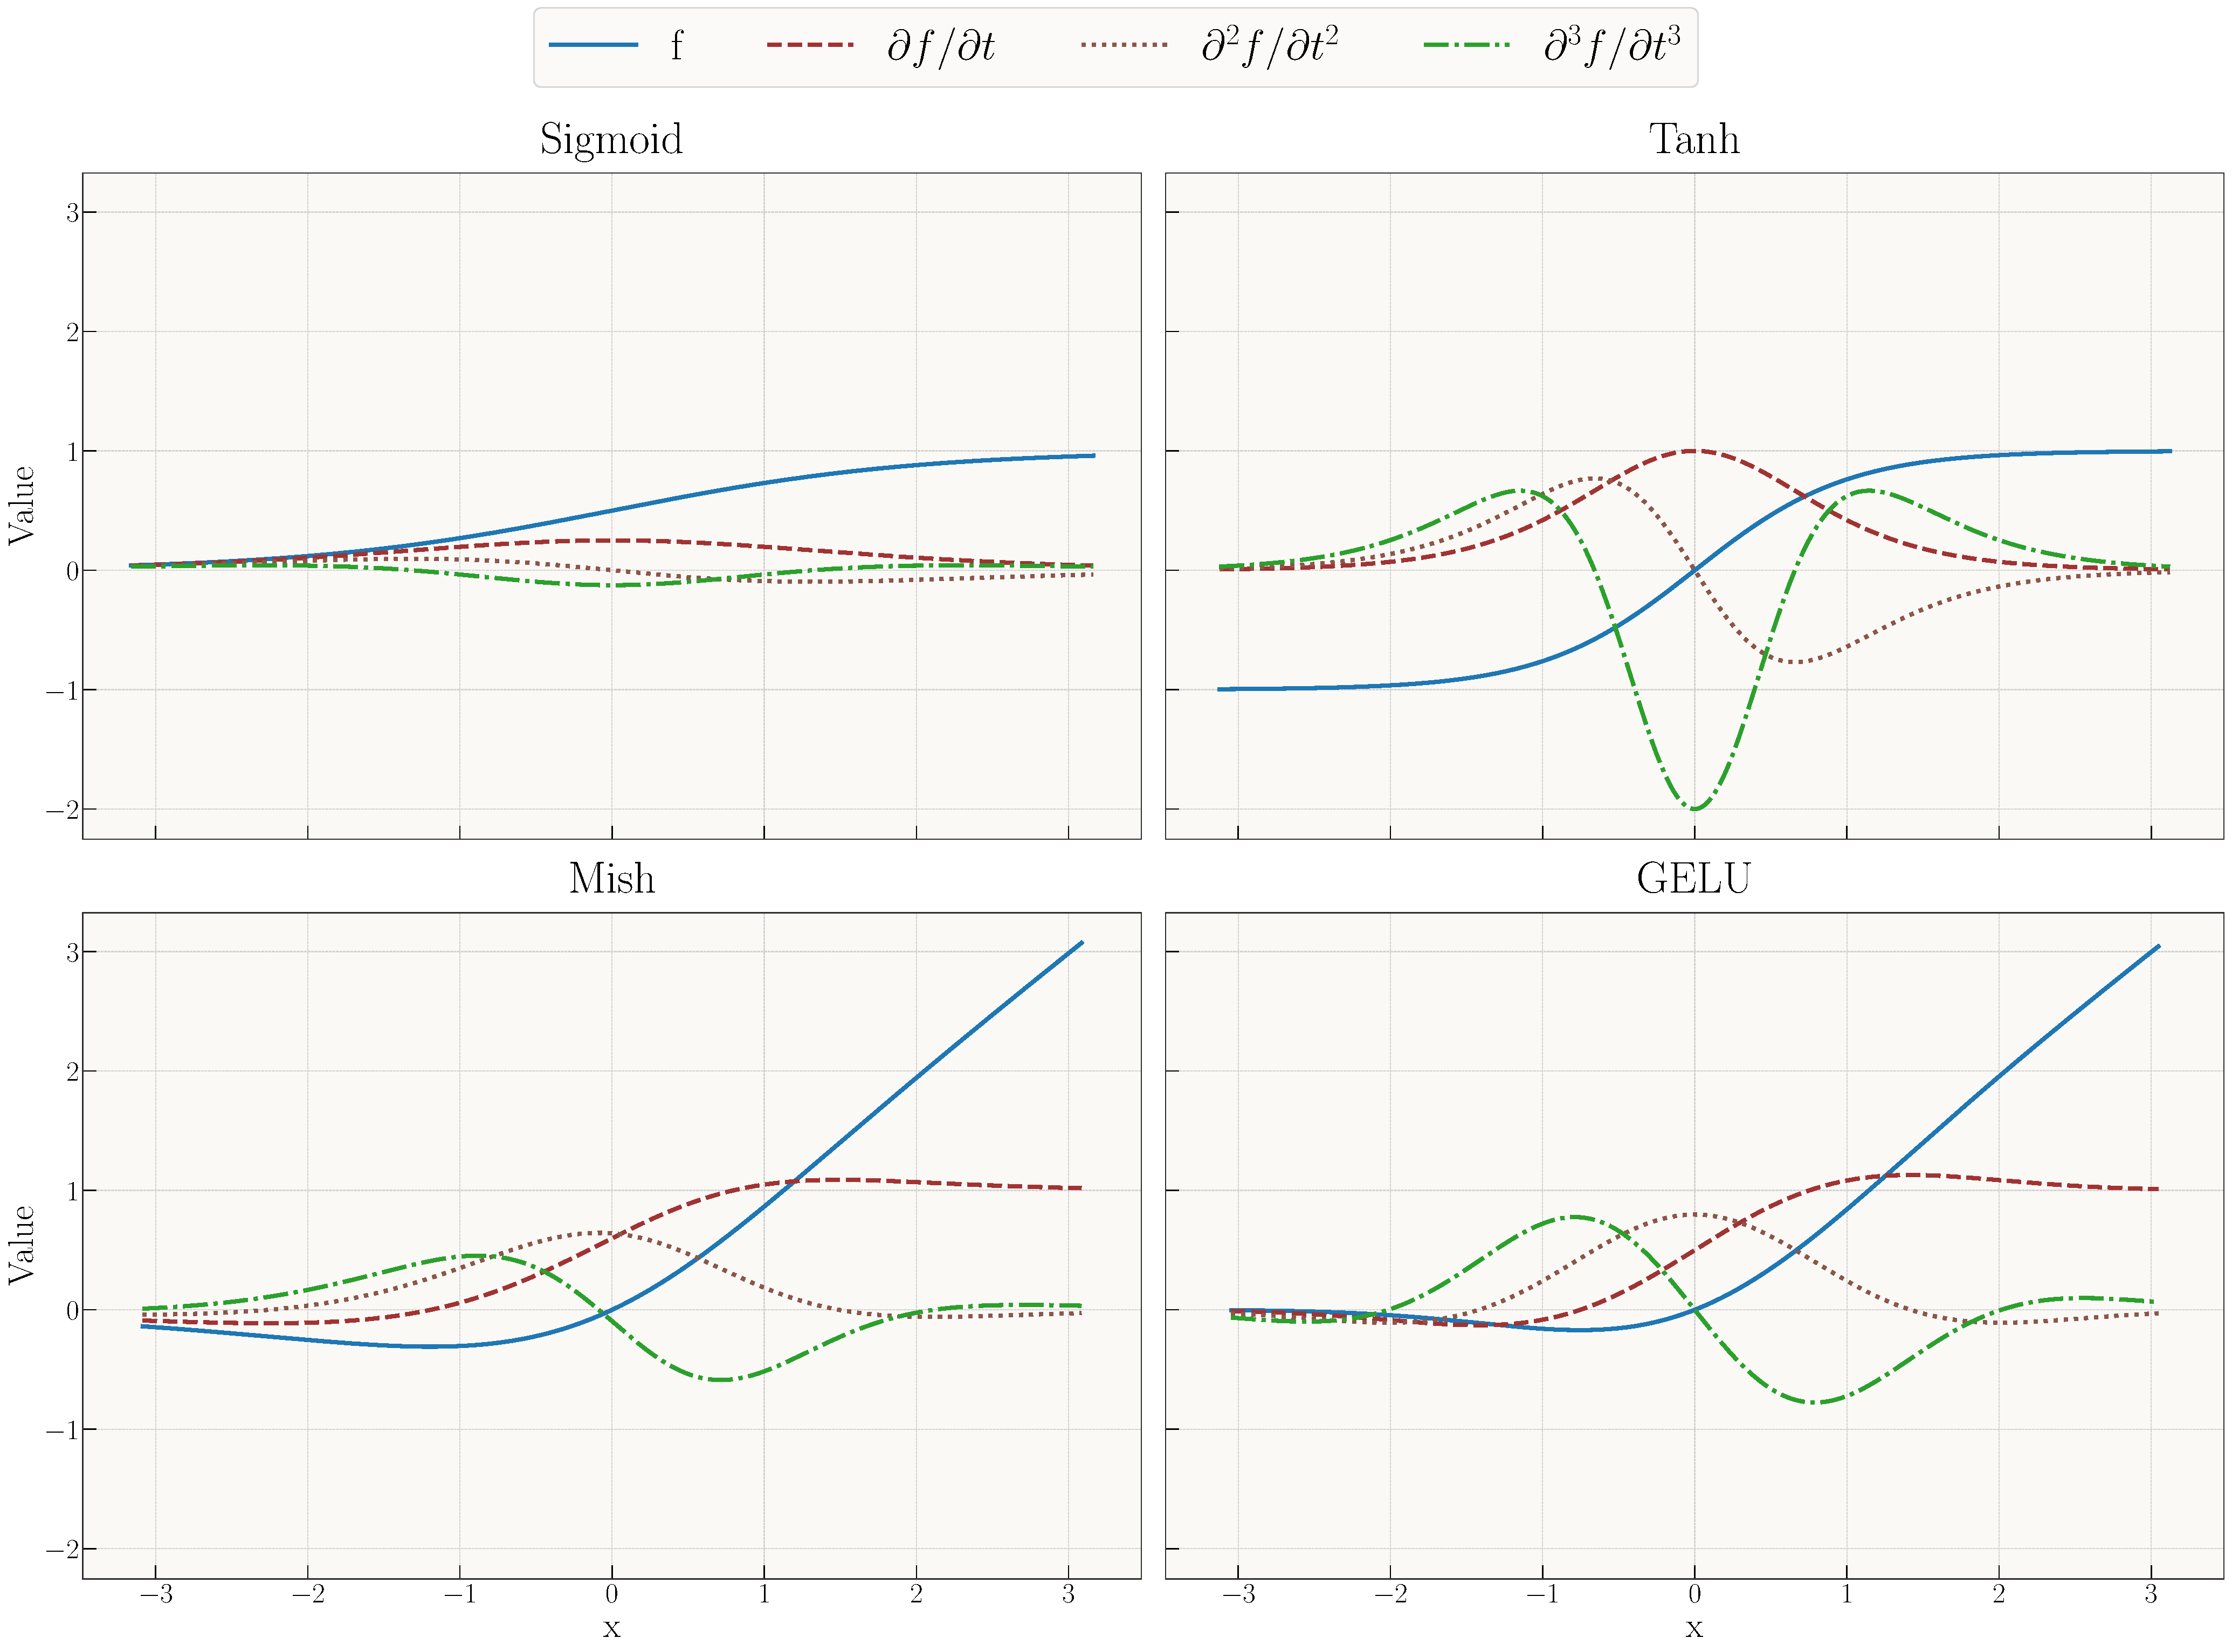
\includegraphics[width=0.8\textwidth]{all_activations_shared_legend.pdf}
  \caption[Activation functions and their first three derivatives]{Common activation functions and their first three derivatives. All of
  GELU, Mish, tanh and the logistic sigmoid are $C^\infty$, so the distinction is not
  smoothness but the \emph{reach} of the higher derivatives: for GELU and Mish the second
  and third derivatives are broad and decay slowly to zero, while for tanh and sigmoid they
  are sharply peaked near the origin and change sign, so curvature accumulates unevenly
  when such units are composed through depth. ReLU is shown for contrast; its second
  derivative is a distribution and it cannot be used in a Laplacian-based objective at all.}
  \label{fig:activation_derivatives}
\end{figure}

\paragraph{Initialisation.}
The standard schemes (Xavier/Glorot, scaling weight variance as $1/(n_{\rm in}+n_{\rm out})$, and Kaiming/He, scaling as $2/n_{\rm in}$ for rectified units) are designed to keep
forward activations and backward gradients from shrinking or exploding through
depth~\cite{GlorotBengio2010-Xavier,HeEtAl2015-KaimingInit}. That is necessary but not
sufficient when the loss contains second derivatives, because a scheme that stabilises
$\partial f/\partial x$ says nothing directly about $\partial^2 f/\partial x^2$. We use
Xavier-style initialisation with the smooth activations above, and---more consequentially
than any initialisation choice---zero-initialise the final layer of the backflow, so that
the ansatz begins exactly at the Slater nodes and the learned nodal deformation grows from
nothing rather than from noise (\S\ref{sec:bf-init}).

None of this makes the Laplacian well conditioned; it only stops the network from making
it worse. The conditioning itself comes from the coordinate scaling, the soft-core pair
features and the analytic cusp of Chapter~\ref{ch:trial_wavefunction}, and is analysed in
Appendices~\ref{app:laplacian} and~\ref{app:coulomb}.


\section{Architectures for many-body wavefunctions}
\label{sec:architectures}

The feed-forward network of the previous section maps a fixed-size input vector to an
output. A many-body wavefunction is not a generic function of such a vector: identical
particles impose a permutation symmetry, and correlation is intrinsically
\emph{relational}---what one particle should do depends on where the others are. A plain
multilayer perceptron acting on the concatenated coordinates
$(\mathbf x_1,\dots,\mathbf x_N)$ respects neither property; it would have to learn the
symmetry from data, and its parameter count would grow with $N$. This section introduces
the two architecture classes that build the required structure in, permutation-invariant pooling and message passing, and situates the specific message-passing network used in
this thesis as one instance of the latter.

\subsection{Permutation symmetry and equivariance}
For identical particles the modulus $|\Psi|$ is invariant under exchange (the sign is
carried by the antisymmetric Slater reference of Chapter~\ref{ch:trial_wavefunction}).
The two learnable objects of the ansatz therefore have distinct symmetry requirements.
A scalar \emph{correlator} $f$ must be permutation-\emph{invariant},
\[
  f(P_\sigma R)=f(R),
\]
while a per-particle \emph{backflow} displacement field $\mathbf g=(\mathbf g_1,\dots,\mathbf g_N)$
must be permutation-\emph{equivariant},
\[
  \mathbf g(P_\sigma R)=P_\sigma\,\mathbf g(R),
\]
for any permutation $\sigma$ (here $P_\sigma$ relabels the particles). Enforcing these by
construction is both more data-efficient than learning them and yields a parameter count
independent of $N$, because the same shared maps are applied to every particle and pair.

\subsection{Permutation-invariant pooling: DeepSets}
The simplest way to build an invariant function is to embed each particle independently
and pool the embeddings symmetrically. This is the DeepSets
construction~\cite{Zaheer2017-DeepSets}: any suitably regular permutation-invariant
function admits the form
\[
  f(R)=\rho\!\Big(\textstyle\sum_i \phi(\mathbf x_i)\Big),
\]
with a per-particle embedding $\phi$, a symmetric pool $\sum_i$, and a readout $\rho$. A
two-body extension encodes pairs, $\phi(\mathbf x_i,\mathbf x_j)$, and pools over them,
capturing pairwise correlation. What characterises this class is that each particle, or pair, is embedded \emph{independently} and only then pooled: no information is exchanged
between particles before the pool. We refer to such networks as \emph{separable}, and
they serve as the non-message-passing baseline for the correlator.

\subsection{Message passing and graph networks}
To let a particle's representation depend on the others' in an iterated, higher-order
way, one places the particles on a graph---nodes are particles, edges are
pairs---and passes learned messages along the edges~\cite{Gilmer2017-MPNN,Battaglia2018-GraphNetworks}.
In a generic round $\ell$, each edge gathers information from its endpoint nodes and each
node aggregates its incoming edge messages,
\[
  \mathbf m_{ij}^{(\ell)} = \phi_e\!\big(\mathbf h_i^{(\ell)},\mathbf h_j^{(\ell)},\mathbf e_{ij}^{(\ell)}\big),
  \qquad
  \mathbf h_i^{(\ell+1)} = \phi_v\!\Big(\mathbf h_i^{(\ell)},\ \textstyle\operatorname*{Agg}_{j\neq i}\mathbf m_{ij}^{(\ell)}\Big),
\]
with shared maps $\phi_e,\phi_v$ and a symmetric aggregation $\operatorname{Agg}$, so that
permutation equivariance holds by construction; a final readout produces an invariant
scalar (correlator) or an equivariant field (backflow). Both DeepSets and message passing
use pairwise information, but only message passing lets that information
\emph{propagate}: after several rounds a particle's representation reflects not just its
neighbours but their neighbours' responses. This iterated propagation is what we call the
\emph{relational channel}, and asking what it buys, in the correlator and in the backflow, is one of the central questions of this thesis. Message passing has been used
in exactly this spirit for neural quantum states of extended fermion
systems~\cite{Pescia2024-MessagePassingNQS,KimEtAl2023-UltracoldFermiNQS}.

\subsection{The CTNN: one message-passing instance}
\label{sec:ctnn-theory}
The message-passing correlator and backflow studied here are realised by a particular
network we refer to as the \emph{CTNN}: a copresheaf-style message-passing network that
maintains explicit \emph{node and edge} features and transports information between them
through learned maps, rather than recomputing and discarding one-shot messages. The
correlator iterates this exchange over a down/up ``V-cycle''; the backflow applies a
single such copresheaf round. Its concrete update equations, hidden dimensions, and
parameter counts are specified in the Methods chapter
(\S\ref{subsec:ctnn-backflow}, Eqs.~\eqref{eq:ctnn-edge}--\eqref{eq:ctnn-node}). Two things follow. First, the CTNN is \emph{one} concrete realisation of
the message-passing class defined above, and the comparison run in this thesis is between two
specific inductive biases---the CTNN against a DeepSets-type separable baseline---not between
the classes they belong to. Conclusions are stated for message passing \emph{as instantiated
by the CTNN, relative to the separable baseline studied here}; whether they generalise to
other message-passing neural quantum states is a plausible extrapolation and not something
these experiments test. Wherever we
contrast a ``message-passing'' network with a ``separable'' one, the separable member is
a DeepSets-type network and the message-passing member is the CTNN. Second, we write
``copresheaf-\emph{style}'' deliberately: the name reflects the node/edge transport
structure of the updates, not a claim to a formal sheaf-theoretic construction.

\subsection{Relevance to the ansatz}
Both learnable objects of the ansatz---the Jastrow correlator and the coordinate
backflow---can be built in either form: as a separable DeepSets-type network, or as the
message-passing CTNN. Holding everything else fixed and varying only this choice isolates
the effect of the relational channel, which Chapter~\ref{ch:kernel} analyses through the
geometry of the tangent kernel introduced in \S\ref{sec:theory-tangent-kernel}.

\section{Approximation theory and its limits}
\label{sec:nn_approximation}

The usual justification for using a neural network as a variational ansatz is that it can
represent anything. That argument needs disposing of early, since this thesis is about what
happens after it stops being relevant.

The universal approximation theorems say that a single hidden layer with a non-polynomial
activation is dense in $C(K)$ on compacta: for any continuous $f$ and any $\varepsilon>0$
there exist a width and a parameter vector achieving
$\sup_{x\in K}|f(x)-f_\theta(x)|<\varepsilon$~\cite{Cybenko1989,HORNIK1991251,LeshnoEtAl1993-NonpolyActivationUniversality}.
They establish one thing, best put negatively: there is no \emph{fundamental}
representability obstruction. They say nothing about the particular $20$k--$236$k networks
used here, nor about whether gradient-based training will find such a representation, at
what sample cost, or how the answer depends on the parameterisation. The existence proofs
are non-constructive, the widths they guarantee are astronomical, and the same function can
be represented by two networks whose optimisation behaviour is entirely different---which is,
in miniature, the comparison Chapter~\ref{ch:kernel} makes.

One further result does more than assert possibility. In high dimension a generic
continuous target requires a network size growing exponentially in $d$, so approximation
alone cannot explain why these methods work at all in $Nd$ dimensions.
The escapes are all statements about \emph{structure}, not capacity: targets of
finite Barron norm admit dimension-independent
rates~\cite{Barron1993-UniversalApprox}; compositional targets admit efficient
representation by deep networks when the composition matches the architecture; and imposing a symmetry removes the redundant
copies the network would otherwise have to learn, reducing the burden on the representation
rather than the dimension of the domain. The last of these is the one we exploit
directly, and the middle one is why the message-passing architectures of
\S\ref{sec:architectures} deserve attention: their usefulness comes from a compositional
form matching the relational structure of the physics, not from added capacity.

The rest of the thesis therefore assumes representability and measures the other things:
trainability, conditioning, and the geometry of the parameterisation.


\section{Residual objectives and their difficulties}
\label{sec:pinns}

In scientific applications the governing equations already encode most of what is known
about a system, and a model fitted only to data throws that information away.
\emph{Physics-informed neural networks} (PINNs)~\cite{raissi2019pinns} put it back by
penalising the residual of the equation itself: for a differential operator $\mathcal N$ and
a network $u_\theta$, the loss is a sampled sum of $|\mathcal N[u_\theta](\xi_j)|^2$ over
collocation points $\{\xi_j\}$, together with boundary and data terms. Training a network
against a differential operator predates the name by two
decades~\cite{Lagaris1998-ANNforODEPDE}; what \cite{raissi2019pinns} added was automatic
differentiation, which evaluates $\nabla u_\theta$ and $\Delta u_\theta$ exactly and cheaply
enough that the residual can drive the optimisation directly.

Four difficulties follow from differentiating through the operator, and each recurs by name
in the results of this thesis~\cite{De_Ryck_2024}.

\emph{Approximation in Sobolev norms.} Universal approximation controls function error in
$L^2$ or $L^\infty$, but a strong residual depends on \emph{derivatives}. Making it small
requires approximation in $W^{\ell,p}$ with $\ell$ the order of the equation, which forces
smooth activations for $\ell\ge2$ and architecture choices that control higher derivatives.
This is why the activation here is chosen for its second derivative, not its values.

\emph{Residual-to-error stability.} A small residual implies a small solution error only
where the forward problem is stable. This is why a small residual is never taken here as
evidence of a good state without an independent energy evaluation.

\emph{Sampling.} Collocation minimises a sampled surrogate of a continuum loss, and the
empirical residual can be small while the population residual is not. In this setting the
question becomes whether an importance-weighted estimator has a finite variance at all,
which is what bounds the Markov-chain-free programme of Chapter~\ref{ch:kernel}.

\emph{Conditioning.} Residual losses couple terms of disparate scale and produce
ill-conditioned gradient dynamics; in the linearised view, convergence is governed by the
spectrum of a problem-dependent kernel. That spectrum is the subject of the entire
tangent-kernel analysis.

The last of these determined the design of the collocation programme. A strong-form residual
that differentiates through the Laplacian meets a structural obstruction as soon as it is
asked to train a nodal surface, because the learning signal lives where $E_L$ diverges. The
weak form keeps the local energy as a detached reward and never differentiates it, and so
avoids the obstruction; Appendix~\ref{app:catch22} shows why, and it is the reason the
collocation programme takes the form it does.

\section{Constraints carried into the method}
\label{sec:ml_summary}

The two traditions of this chapter and the last have been describing the same objects in
different words. The quantum geometric tensor of variational Monte Carlo is the Fisher
metric of information geometry; stochastic reconfiguration is natural-gradient descent
under it; the neural tangent kernel is that metric's Gram dual; and the sampling measure a
physicist chooses for a Metropolis chain is what a statistician calls a proposal
distribution. Neither community needs the other's vocabulary in order to do its own work, which is why
the identifications are easy to miss. They matter here because the architecture determines
the spectrum of that metric, the optimiser inverts it, and the sampling measure determines
how well it can be estimated.

Four properties of this problem bear on that metric.

\emph{The objective contains a second-order operator.} The local energy carries a
Laplacian, so training differentiates through second derivatives of the network. This is
what dictates smooth activations, controlled initialisation, and a determinant that is
never asked to do anything violent (\S\ref{sec:ffnn}).

\emph{The interaction is singular, and the state carries nodes.} The Coulomb term diverges
at coalescence, and the trial function vanishes on a surface whose location is itself being
learned. Both are places where $E_L=\hat H\Psi/\Psi$ can blow up, and the cusp conditions
of \S\ref{subsec:cusp} say that the first divergence can be cancelled analytically if the
short-range form is built in, not learned.

\emph{The measure is part of the method.} The objective is an expectation under
$|\Psi_\theta|^2$, so the sampling distribution enters the gradient, the metric, and the
estimate of both. Whether that metric can be estimated at all turns out to decide whether
preconditioning helps or hurts (\S\ref{sec:theory-tangent-kernel}).

\emph{Correlation is relational.} What one electron should do depends on where the others
are, and the two architecture classes of \S\ref{sec:architectures} differ precisely in how
far that dependence is allowed to propagate.

The first two are met by construction in Chapter~\ref{ch:trial_wavefunction}, which
hard-wires antisymmetry and the cusp and conditions the geometry so that the learned part
can remain small and smooth. The third is treated in Chapter~\ref{ch:optimisation}, where
the sampling measure is a design variable rather than a fixed background. The fourth is not
settled here: both architectures are constructed, and the comparison between them is
reported in Chapter~\ref{ch:kernel}.



\part{Methods}
\chapterepigraph{No great thing is created suddenly, any more than a bunch of
grapes or a fig.}{Epictetus}{\textit{Discourses}}

\begingroup
\let\clearpage\relax
\let\cleardoublepage\relax
\chapter{The trial wavefunction}
\label{ch:trial_wavefunction}
\endgroup

The trial state is constructed to satisfy fermionic antisymmetry and the electron--electron
cusp analytically, and to keep the learned terms smooth under the Laplacian. Antisymmetry
requires a determinant. The Coulomb divergence admits an analytic cancellation, so it is imposed, not learned. Second derivatives enter the loss, so the features fed to the
network are bounded and smooth and the coordinates are scaled to keep those derivatives
$\mathcal{O}(1)$ across three decades of confinement. The form of the learned part is not
fixed by these constraints; both candidate architectures are constructed here and compared
in Chapter~\ref{ch:kernel}. Unless stated otherwise we work in atomic units.

\section{Preliminaries}
\label{sec:setup}

\paragraph{Hamiltonian and units.}
We study $N$ spin-$\tfrac12$ fermions in two spatial dimensions confined by a harmonic trap
and interacting via Coulomb repulsion,
\begin{equation}
\label{eq:dot-h}
H \;=\; \sum_{i=1}^N \Big( -\tfrac12 \nabla_{\mathbf r_i}^2 + \tfrac12 \,\omega^2 r_i^2 \Big)
\;+\; \sum_{1\le i<j\le N} \frac{1}{|\mathbf r_i-\mathbf r_j|},
\qquad (\hbar=m_e=e=1).
\end{equation}
Spin does not appear in $H$; eigenstates factorize into a spatial function with good $L_z$ and a
spin function with good $(S,S_z)$.

\paragraph{Coordinates and scaling.}
We collect positions as $R=(\mathbf r_1,\ldots,\mathbf r_N)\in\mathbb R^{2N}$ and use trap scaling
$\tilde{\mathbf r}_i=\sqrt{\omega}\,\mathbf r_i$, $\tilde{R}=\sqrt{\omega}\,R$. This aligns typical
length scales to $\mathcal O(1)$, improves conditioning of second derivatives, and makes the
noninteracting ground state $\omega$-independent. When useful, we also use pair distances
$r_{ij}=|\mathbf r_i-\mathbf r_j|$ and their scaled versions $\tilde r_{ij}=|\tilde{\mathbf r}_i-\tilde{\mathbf r}_j|$.

\paragraph{Sectors and focus.}
We primarily report \emph{closed-shell} cases (unique spin singlet at the noninteracting level).
Open shells introduce a degenerate manifold and additional choices for the reference; we keep this
to brief remarks only where needed.

\paragraph{Spin–orbitals and basis.}
One-particle spatial orbitals are the Cartesian two-dimensional harmonic-oscillator
eigenstates $\{\phi_{n_x n_y}(\mathbf r)\}$ with $E_{n_x n_y}=\omega(n_x+n_y+1)$,
$n_x,n_y\in\mathbb N_0$ (the basis used in the implementation; for the closed shells studied
it spans the same filled shells as any complete basis of those shells). Spin–orbitals
are $\varepsilon_\alpha(x)=\phi_{n_x n_y}(\mathbf r)\chi_\sigma(s)$, $\sigma\in\{\uparrow,\downarrow\}$.

% ==========================================================

\section{Overview of the ansatz}
\label{sec:ansatz}
Our trial state combines exact antisymmetry, an analytic short-range cusp, and a compact
neural residual, while optionally evaluating the Slater determinant on backflowed coordinates:
\begin{align}
  \Psi_{\theta,\beta}(R)
  &= \mathrm{SD}\big(\tilde{R}'\big)\;
     \exp\!\Big(
       \sum_{i<j} u_{\sigma_i \sigma_j}(r_{ij})
       + W_\theta(\tilde{R})
     \Big),\label{eq:ansatz-overall} \\
  \tilde{R}' &= \tilde{R} + \Delta_\beta(\tilde{R}).\label{eq:bf-coords}
\end{align}
Here $\mathrm{SD}$ enforces antisymmetry; $u$ hard-wires the Kato cusp; $W_\theta$ (the NQS correlator) learns smooth
medium/long-range structure; and $\Delta_\beta$ (backflow) adjusts the nodes by smoothly warping the coordinates used
inside the determinants; its per-particle displacements $\Delta_{\beta,i}$ are written
$\Delta\mathbf{x}_i$ in the results chapters. We deliberately feed the NQS with $\tilde{R}$ (not $\tilde{R}'$) to avoid self-reinforcing feedback
and keep local-energy variance low.

\paragraph{Design principles.}
(i) \emph{Separate guaranteed physics from learned details:} antisymmetry and the cusp are hard-wired; the network learns the rest.
(ii) \emph{Condition the geometry:} work in trap units and use soft-core pair features so that first/second derivatives are bounded.
(iii) \emph{Keep the learned object small and smooth:} once the cusp is explicit, a compact NQS suffices across $(N,\omega)$.

\section{Slater reference}
\label{subsec:slater}
For closed shells we use a restricted product of spin-block determinants of the lowest $N/2$ harmonic oscillator orbitals (trap units):
\begin{equation}
  \mathrm{SD}(\tilde{R})
  =
  \det\!\big[\phi_a(\tilde{\mathbf r}_i)\big]_{i\in\uparrow,\;a\le N/2}\;
  \det\!\big[\phi_a(\tilde{\mathbf r}_j)\big]_{j\in\downarrow,\;a\le N/2}.
  \label{eq:slater}
\end{equation}
The correlator reweights amplitudes \emph{within} nodal pockets; without backflow, the nodes are those of~\eqref{eq:slater}.

\section{Neural correlator $W_\theta$}
\label{subsec:nqs}
As with the backflow, the correlator comes in two forms that are compared directly in
\S\ref{sec:kernel-q1}: a \emph{separable} network that encodes particle- and
pair-features independently and pools them, and a copresheaf \emph{message-passing}
(CTNN) network. We describe the separable network first, since it is the baseline and supplies the safe features and analytic cusp shared by both, and then the message-passing one.

\subsection{Separable correlator (DeepSets baseline)}
\label{subsec:separable-correlator}
The separable NQS aggregates \emph{particlewise} and \emph{pairwise} embeddings with permutation-invariant pooling and appends two global
statistics, all in $\tilde{R}$. A core safety requirement is that pair channels satisfy $d s_k/d\tilde r \to 0$ as $\tilde r\to 0$
so that $W_\theta$ never injects spurious $1/\tilde r$ terms into $\nabla\log\Psi$ or $\Delta\log\Psi$.

\subsubsection{Particle branch (DeepSets).}
This part of the network is typically referred to as Deep Sets~\cite{Zaheer2017-DeepSets}. The permutation invariance of quantum many-body mechanics is naturally captured by this architecture. 
A neural network $\phi$ creates a latent embedding for each particle individually. All embeddings are pooled together to form a global representation, which is used later in the readout. Formally, we have
\[
  \mathbf h_i^\phi=\phi(\tilde{\mathbf x}_i)\in\mathbb R^{d_L},\qquad
  \overline{\mathbf h}^{\phi}=N^{-1}\sum_i \mathbf h_i^\phi\in\mathbb R^{d_L}.
\]

\subsubsection{Pair branch (soft-core, even channels).}
Although the particle branch could theoretically produce pair correlations, in practice it struggles to represent sharp near-field structure. We therefore add a dedicated pair branch that builds features from interparticle distances.
This network processes all pairs $(i,j), i\ne j$ individually and pools the resulting latent embeddings. 
The problem is that raw distances $\tilde r_{ij}$ have unbounded derivatives at coalescence, which destabilizes Laplacian evaluations. We therefore build \emph{safe} pair features with bounded first and second derivatives as $\tilde r\to 0$.
With $\tilde r^{\rm soft}=\sqrt{\tilde r^2+\varepsilon^2}$ ($\varepsilon\!\in[0.15,0.30]$ in trap units), we build six “safe” features
\begin{align}
  s_1 &= \log\!\big(1+(\tilde r^{\rm soft}/\varepsilon)^2\big),\quad
  s_2 = \tfrac{\tilde r^{2}}{\tilde r^{2}+\varepsilon^2},\quad
  s_3 = (\tilde r^{\rm soft}/\varepsilon)^{2}\exp[-(\tilde r^{\rm soft}/\varepsilon)^{2}], \notag\\
  \mathrm{rbf}_g &= \exp(-g\,s_1),\quad g\in\{0.25,1,4\},\qquad
  \mathbf u_{ij}=[s_1,s_2,s_3,\mathrm{rbf}_{0.25},\mathrm{rbf}_{1},\mathrm{rbf}_4]\in\mathbb R^{6}.
  \label{eq:safe-feats}
\end{align}
An MLP $\psi$ maps $\mathbf u_{ij}\mapsto\mathbf h^{\psi}_{ij}\in\mathbb R^{d_L}$. A short-range gate
\[
  \chi(\tilde r)=\frac{\tilde r^{2}}{\tilde r^{2}+r_g^{2}},\quad r_g\approx 0.3,\quad \chi(0)=\chi'(0)=0,
\]
suppresses learned responses \emph{at} coalescence; downstream we use
$\chi\,\mathbf h^\psi_{ij}$.

\subsection{Analytic short-range cusp (shared)}
\label{subsec:cusp-implementation}
The analytic cusp below is shared by both correlator variants (and is independent of the
backflow). Because the safe features are necessary in the pair branch, the NQS cannot represent the Kato cusp condition exactly.
We therefore add an analytic cusp term to the exponent in~\eqref{eq:ansatz-overall},
written in \emph{physical} coordinates so that its slope at contact is manifestly
correct:
\begin{equation}
  u_{\sigma\sigma'}(r)
  =
  \gamma_{\sigma\sigma'}\, r\, e^{-r/a_{\rm ho}},
  \qquad a_{\rm ho}=1/\sqrt{\omega},
  \qquad
  \gamma_{\uparrow\downarrow}=\tfrac{1}{d-1},\quad
  \gamma_{\uparrow\uparrow}=\tfrac{1}{d+1}.
  \label{eq:cusp}
\end{equation}
Because the linear prefactor is the physical separation $r$, the slope at contact is
$\partial_r u|_{0}=\gamma_{\sigma\sigma'}$, exactly the Kato condition in general $d$;
for $d=2$ this gives $\gamma_{\uparrow\downarrow}=1$ and $\gamma_{\uparrow\uparrow}=\tfrac13$,
the standard two-dimensional quantum-dot values, derived---including the parallel-spin
case, where antisymmetry already forces a linear node---in
Appendix~\ref{app:coulomb:cusp}. Only the exponential taper carries the trap length
$a_{\rm ho}$, suppressing long-range interference so the NQS need not unlearn cusp
structure at medium and long range; in trap units ($\tilde r=\sqrt{\omega}\,r$) the same
term reads $u=(\gamma_{\sigma\sigma'}/\sqrt{\omega})\,\tilde r\,e^{-\tilde r}$.


\subsection{Separable readout}
With contributions from the particle and pair branches, we form a global representation for the final readout. In addition to the pooled embeddings $\overline{\mathbf h}^\phi$ and $\overline{\mathbf h}^\psi$, we also include two global statistics that help the network gauge overall system size and density.
We average pairs by default or apply degree-normalised radial attention
\[
  w_{ij}=\exp[-(\tilde r_{ij}/r_c)^p],\quad
  \hat w_{ij}=w_{ij}\Big/\sum_{k\ne i}w_{ik},\quad
  (r_c,p)=(0.4,6),
\]
then form $g_i=\sum_{j\ne i}\hat w_{ij}\,\mathbf h^\psi_{ij}$ and $\overline{\mathbf h}^\psi=N^{-1}\sum_i g_i$.
Two system-level scalars in trap units,
\[
  \mathbf g(\tilde{R})=
  \Big[\tfrac{1}{Nd}\sum_i\|\tilde{\mathbf x}_i\|^2,\;
       \tfrac{2}{N(N-1)}\sum_{i<j}s_1(\tilde r_{ij})\Big]\in\mathbb R^2,
\]
are concatenated with $\overline{\mathbf h}^{\phi}$ and $\overline{\mathbf h}^{\psi}$ and mapped to a scalar by a tiny MLP $\rho$:
\begin{equation}
  W_\theta(\tilde{R})
  =
  \rho\!\Big(\overline{\mathbf h}^{\phi}\ \|\ \overline{\mathbf h}^{\psi}\ \|\ \mathbf g(\tilde{R})\Big).
  \label{eq:nqs-readout}
\end{equation}

\subsection{Message-passing correlator (CTNN)}
\label{subsec:ctnn-correlator}
The message-passing correlator keeps the same node/edge
embeddings, safe pair features, and analytic cusp, but replaces the independent pooling of
the separable network with the copresheaf transport of \S\ref{sec:ctnn-theory}: at each
round the endpoint nodes are transported into an edge update and the updated edges are
transported back and aggregated onto the nodes,
\begin{equation}
  \mathbf h_{ij} \mathrel{+}= F_e\!\big(\mathbf h_{ij}\,\|\,\rho_{v\to e}\mathbf h_i\,\|\,\rho_{v\to e}\mathbf h_j\big),
  \qquad
  \mathbf h_i \mathrel{+}= F_v\!\Big(\mathbf h_i\,\|\,\operatorname*{Agg}_{j\neq i} w_{ij}^{\rm spin}\,\rho_{e\to v}\mathbf h_{ij}\Big),
  \label{eq:ctnn-corr-step}
\end{equation}
with residual updates and per-round transport maps. Unlike the single-round backflow, the
correlator stacks these rounds in a multiscale ``V-cycle'': $n_{\downarrow}$ down-pass
rounds, a linear coarsening to a bottleneck width, then $n_{\uparrow}$ up-pass rounds with
skip connections back to the down-pass features (defaults $n_{\downarrow}=n_{\uparrow}=2$).
A permutation-invariant readout over the final node and edge statistics returns the scalar
$W_\theta(\tilde R)$, exactly as in~\eqref{eq:nqs-readout}. Holding the Slater reference,
cusp, and training fixed and swapping only the separable readout for this V-cycle isolates
the relational channel analysed in \S\ref{sec:kernel-q1}.

\section{Backflow}
\label{subsec:backflow-method}

Backflow deforms the coordinates \emph{used only inside the Slater reference} so that the nodal surface can adapt to interparticle correlations:
\begin{equation}
  \tilde{R}' \;=\; \tilde{R} + \Delta_\beta(\tilde{R}) ,
  \qquad
  \Psi_{\theta,\beta}(R) \;=\; \mathrm{SD}(\tilde R')\;
  \exp\!\Big(\sum_{i<j} u_{\sigma_i\sigma_j}(r_{ij}) + W_\theta(\tilde R)\Big).
  \label{eq:bf-def}
\end{equation}
The correlator $W_\theta$ and cusp $u$ are evaluated on $\tilde R$ to avoid feedback loops in the local energy; only the determinant ``sees'' $\tilde R'$.
This choice cleanly separates (i) amplitude reweighting within nodal pockets (handled by $u+W_\theta$) from (ii) nodal \emph{geometry} (handled by backflow).

\paragraph{Design goals.}
(i) \emph{Stability near coalescence:} messages are built from mollified radii and
short-range gates so that $\partial \Delta_\beta/\partial \tilde r$ stays bounded;
(ii) \emph{Permutation symmetry:} permutation equivariance holds by construction (shared
maps and symmetric aggregation);
(iii) \emph{Close to identity at initialisation:} a zero-initialised last layer and a
positive learnable scale keep $\Delta_\beta\!\approx\!0$ at the start.
Rotational symmetry, by contrast, is only \emph{approximate}: the displacement head reads
out a $d$-vector from node features that include the raw coordinates, so the map is not
rotation-equivariant by construction, and it is encouraged instead by the
geometry-based edge features and by rotationally-augmented sampling. A global translation
is not a symmetry of the trap in any case; the zero-mean projection~\eqref{eq:bf-com} is a
regulariser that removes a spurious centre-of-mass drift, not an imposed physical symmetry.

We study \emph{two} backflow architectures. Both map the configuration to a per-particle
displacement field and share the output bounding, spin masking, and centre-of-mass
projection below; they differ only in how a particle's displacement is made to depend on
the others. The conventional network is the baseline of the architecture comparison in
Chapter~\ref{ch:kernel}; the copresheaf \textsc{CTNN} is the production ansatz.

\subsection{Conventional backflow (single-round messages)}
The baseline uses a single round of pairwise messages. For
each ordered pair $(i,j)$ with $i\neq j$,
\begin{equation}
  \mathbf m_{ij}
  = \phi_\beta\!\big(
      \tilde{\mathbf x}_i,\ \tilde{\mathbf x}_j,\ \mathbf r_{ij},\
      \tilde r_{ij}^{\rm soft},\ (\tilde r_{ij}^{\rm soft})^2
    \big)\cdot w_{ij}^{\rm spin},
  \qquad \tilde r_{ij}^{\rm soft}=\sqrt{\tilde r_{ij}^2+\varepsilon_{\rm bf}^2},
  \label{eq:bf-message}
\end{equation}
with $\phi_\beta$ a small MLP and $w_{ij}^{\rm spin}\in\{0,1\}$ a spin mask (same-spin only
or all pairs). Messages are aggregated to a node state and a node network returns the
displacement,
\begin{equation}
  \mathbf m_i = \operatorname*{Agg}_{j\neq i}\mathbf m_{ij},
  \qquad
  \delta\tilde{\mathbf x}_i = \psi_\beta\!\big(\tilde{\mathbf x}_i \,\|\, \mathbf m_i\big),
  \qquad \mathrm{Agg}\in\{\mathrm{sum},\mathrm{mean},\mathrm{max}\}.
\end{equation}
There is no persistent edge state: each message is recomputed from the raw geometry and
discarded after aggregation.

\subsection{CTNN backflow (copresheaf)}
\label{subsec:ctnn-backflow}
The message-passing architecture instead maintains
explicit \emph{node and edge} features and transports information between them through
learned linear maps---the copresheaf-style step of \S\ref{sec:ctnn-theory}. Node features
are embedded from the position and a spin scalar, edge features from the relative geometry,
\begin{equation}
  \mathbf h_i^{(0)} = W_v\,[\tilde{\mathbf x}_i,\, s_i],
  \qquad
  \mathbf h_{ij}^{(0)} = \mathrm{MLP}_e\!\big(\mathbf r_{ij},\, |\mathbf r_{ij}|,\, |\mathbf r_{ij}|^2\big).
\end{equation}
A node-to-edge transport $\rho_{v\to e}$ feeds the endpoint nodes into an edge update; an
edge-to-node transport $\rho_{e\to v}$ returns the updated edges to the nodes, which are
refined by a residual node update; a linear head reads out the displacement:
\begin{align}
  \mathbf h_{ij}' &= \mathrm{MLP}_e'\!\big(\mathbf h_{ij}^{(0)}\,\|\,\rho_{v\to e}\mathbf h_i^{(0)}\,\|\,\rho_{v\to e}\mathbf h_j^{(0)}\big),
  \label{eq:ctnn-edge}\\
  \mathbf m_i &= \operatorname*{Agg}_{j\neq i} w_{ij}^{\rm spin}\,\rho_{e\to v}\big(\mathbf h_{ij}'\big),
  \label{eq:ctnn-agg}\\
  \mathbf h_i &= \mathbf h_i^{(0)} + \mathrm{MLP}_v\!\big(\mathbf h_i^{(0)}\,\|\,\mathbf m_i\big),
  \qquad
  \delta\tilde{\mathbf x}_i = W_{\!\Delta}\,\mathbf h_i.
  \label{eq:ctnn-node}
\end{align}
The learned transport maps $\rho_{v\to e},\rho_{e\to v}$ are the channel whose ablation
collapses the backflow at the Wigner crystal (Chapter~\ref{ch:kernel}). The backflow uses a
single copresheaf round; the message-passing \emph{correlator} of the architecture
comparison (\texttt{CTNNJastrowVCycle}) iterates the same style of update over a down/up
``V-cycle''.

\subsection{Constraints, symmetries and scaling}
\label{sec:bf-init}
Both variants take inputs in trap units ($\tilde{\mathbf x}=\sqrt{\omega}\,\mathbf x$), bound
the displacement, and start at the Slater nodes,
\begin{equation}
  \Delta_\beta(\tilde R)\;=\;\tanh\!\big(\delta\tilde X\big)\cdot s_\beta,
  \qquad s_\beta=\mathrm{softplus}(s_\beta^{\rm raw})>0,
  \label{eq:bf-bound-scale}
\end{equation}
with the last linear layer zero-initialised so that $\Delta_\beta\!\approx\!0$ initially and
$s_\beta$ initialised in $[0.02,0.10]$. This parameterisation stabilises the SR and energy
tails and protects the Laplacian.

Near coalescence raw $1/\tilde r$ factors make $\nabla\!\cdot\!\Delta_\beta$ spiky. We
mollify $\tilde r_{ij}$ as in \eqref{eq:bf-message} and optionally gate the message,
\begin{equation}
  \chi_{\rm bf}(\tilde r_{ij})=\frac{\tilde r_{ij}^2}{\tilde r_{ij}^2+r_g^2},
  \qquad \chi_{\rm bf}(0)=\chi'_{\rm bf}(0)=0,\quad r_g\approx 0.3,
  \label{eq:bf-gate}
\end{equation}
or use degree-normalised radial attention $\hat w_{ij}=w_{ij}/\sum_{k\neq i}w_{ik}$ with
$w_{ij}=\exp[-(\tilde r_{ij}/r_c)^p]$. Either keeps the learned response smooth at contact and
limits the backflow's contribution to the local-energy variance. The mollification scale
$\varepsilon_{\rm bf}=10^{-6}$ is fixed, not tuned, and is a numerical guard rather
than a modelling choice: $\sqrt{\tilde r^2+\varepsilon_{\rm bf}^2}$ differs from $\tilde r$ by
less than $\varepsilon_{\rm bf}$ everywhere, so it changes no value the network can resolve
and exists only to keep $\nabla\tilde r$ finite at exact coincidence. The physical short-range
scale is instead the pair-feature softening $\varepsilon\in[0.15,0.30]$ of
\eqref{eq:safe-feats}, four to five orders of magnitude larger.

Permutation symmetry is automatic. To remove a spurious centre-of-mass drift the flow is
projected to zero mean,
\begin{equation}
  \Delta_\beta \;\leftarrow\; \Delta_\beta \;-\; \frac{1}{N}\sum_{i=1}^N \Delta_{\beta,i},
  \label{eq:bf-com}
\end{equation}
taken over particles within each configuration, not across the batch. Messages are
built from relative vectors $\mathbf r_{ij}$, but the map is not translation-invariant or
rotation-equivariant by construction, since the displacement head reads a $d$-vector from
absolute coordinates. The two variants apply the projection at different points: the
copresheaf network applies \eqref{eq:bf-com} inside its forward pass, while the conventional
network returns the raw displacement and the caller projects when $\tilde R'$ is formed. The
shifted coordinates are identical either way, but a diagnostic evaluated on a network's
\emph{returned} field sees a centre-of-mass component in one case and not the other, which is
why the two rank columns of \S\ref{sec:kernel-q1b} sit under ceilings differing by two.

Because only the determinant is evaluated at $\tilde R'$, backflow moves the \emph{nodes}
while the correlator exponent stays on $\tilde R$, and no Jacobian term arises. This
Feynman--Cohen construction~\cite{FeynmanCohen1956-Backflow} targets fixed-node error
directly; its modern quantum-Monte-Carlo form is due to Holzmann and
Ceperley~\cite{HolzmannCeperley2003-Backflow}. Compute and memory scale as
$O(BN^2(d+H))$ for batch size $B$ and hidden width $H$, which is what limits $N$ in practice.


\section{Architecture sizes and hyperparameters}
\label{sec:hyperparameters}
Table~\ref{tab:hyperparams} collects the representative settings. The two comparisons in
Chapter~\ref{ch:kernel} stand on different footings in this respect.

The \emph{correlator} comparison is capacity-controlled. The two variants are held at
comparable parameter counts, so a difference in outcome cannot be attributed to one simply
being larger, and where \S\ref{sec:kernel-q1a} departs from matched capacity it does so in
the \emph{separable} network's favour, scaling it from $20$k to $164$k parameters against a
fixed $80$k message-passing network without closing the gap.

The \emph{backflow} comparison is not. At equal width the copresheaf network is intrinsically
the heavier object---it carries a persistent edge state where the conventional network carries
only a per-particle aggregate---so at the shared production setting (message width $128$,
node MLP $128\times3$) it holds $182$k parameters against $51$k, a factor of $3.6$. No
matched backflow pair was trained. What separates architecture from capacity there is
therefore not a matched control but the conventional network's own behaviour across
$\omega$, which \S\ref{sec:kernel-q1b} sets out where the measurement is reported. All settings below are those of the accompanying code
the accompanying code.

\begin{table}[htbp]\centering
\caption[Architecture and training hyperparameters]{The three sets of models trained in this
thesis. They exist for different purposes and are never compared with one another. Widths are
hidden dimensions; ``rounds'' are message-passing steps ($n_\downarrow{+}n_\uparrow$ for the
V-cycle). Within the architecture study the correlator variants are not capacity-matched,
which is why \S\ref{sec:kernel-q1a} also reports the matched $89.4$k separable network and
the full $20$k--$164$k ladder; the backflow variants are not matched either, and cannot be at
equal width, for the reason given above. Settings follow the accompanying code
(\texttt{scripts/run\_depth\_analysis.py}, \texttt{scripts/source\_state\_check.py}).}
\label{tab:hyperparams}
\setlength{\tabcolsep}{5pt}
\renewcommand{\arraystretch}{1.25}
\begin{tabular}{@{}p{0.165\linewidth} p{0.335\linewidth} p{0.30\linewidth} r@{}}
\hline
Programme & Correlator & Backflow & Total \\
\hline
Physics production (\S\ref{sec:energy-overview})
  & separable; width $128$, $2$ layers; $54$k
  & conventional; msg $128$, node $128\times3$; $51$k & $105$k \\
  & \emph{(as above)} & message-passing; same widths; $182$k & $236$k \\
\hline
Architecture study (\S\ref{sec:kernel-q1})
  & separable; pair-MLP $64\times4$, out $32$; $47.7$k
  & \multirow{2}{*}{\emph{as production; not matched}} & --- \\
  & message-passing; node/edge $32$, bottleneck $16$, $2{+}2$ rounds; $79.8$k & & --- \\
\hline
Collocation (\S\ref{sec:kernel-mcmcfree})
  & message-passing V-cycle; $25$k & none & $25$k \\
  & \emph{(as above)} & copresheaf; $h_{\rm bf}{=}128$; $+24$k & $49$k \\
\hline
\end{tabular}

\medskip
\small\noindent Readout for every correlator: hidden $64$, $2$--$3$ layers, SiLU.
Optimiser: Adam at $\mathrm{lr}=5\times10^{-4}$ (backflow) and $5\times10^{-5}$ (Jastrow);
CG-SR with Tikhonov damping $\lambda$, a trust-region cap and CG restarts. Collocation batch
$n_{\rm coll}\sim3\times10^{3}$ with oversampling $m=8$--$16$; the collocation families are
described further in \S\ref{subsec:colloc-families}.
\end{table}


\paragraph{Implementation correspondence.} For replication: the separable correlator is
\texttt{PINN} and the message-passing one \texttt{CTNNJastrowVCycle}; the conventional
backflow is \texttt{BackflowNet}, whose $\phi_\beta$ and $\psi_\beta$ are its message and
node MLPs, and the copresheaf backflow is \texttt{CTNNBackflowNet}, whose embeddings,
transport maps and update MLPs realise \eqref{eq:ctnn-edge}--\eqref{eq:ctnn-node}.
Aggregation is selectable (\texttt{sum|mean|max}); the bounded output of
\eqref{eq:bf-bound-scale} is \texttt{out\_bound="tanh"} with
$s_\beta=\mathrm{softplus}(\texttt{bf\_scale\_raw})$. The comparison tiers are produced by
\texttt{scripts/run\_depth\_analysis.py} and the production widths by
\texttt{scripts/source\_state\_check.py}. Schedule and solver options carry the names
\texttt{alpha\_start}, \texttt{alpha\_end}, \texttt{alpha\_decay\_frac},
\texttt{max\_param\_step}, \texttt{damping}, \texttt{micro\_batch} and \texttt{grad\_clip}.

\chapter{Optimisation}
\label{ch:optimisation}
\label{ch:optimization}

\section{Primary objective and two–stage training}
\label{sec:opt-overview}

Given a parameterised wavefunction $\Psi_\theta$, the variational ground–state energy is
\begin{equation}
E(\theta)
=\frac{\langle\Psi_\theta|H|\Psi_\theta\rangle}{\langle\Psi_\theta|\Psi_\theta\rangle}
=\mathbb{E}_{\tilde{R}\sim \pi_\theta}\!\big[E_L(\tilde{R})\big],
\qquad
\pi_\theta(\tilde{R})=\frac{|\Psi_\theta(\tilde{R})|^2}{\int |\Psi_\theta|^2}.
\end{equation}
The local energy is evaluated in \emph{physical} coordinates, consistently with the
Hamiltonian~\eqref{eq:dot-h},
\begin{equation}
\label{eq:local-energy}
E_L(R)
= -\tfrac12\sum_{i=1}^N\!\Big[\Delta_{\mathbf r_i}\ln\Psi_\theta + \|\nabla_{\mathbf r_i}\ln\Psi_\theta\|^2\Big]
+\tfrac{1}{2}\,\omega^2\sum_{i=1}^N r_i^2
+\sum_{i<j}\frac{1}{r_{ij}},
\end{equation}
and the zero–variance principle holds: $\mathrm{Var}_{\pi_\theta}[E_L]=0$ iff $\Psi_\theta$ is an eigenstate.
The network \emph{features} are computed in trap units $\tilde{\mathbf r}=\sqrt{\omega}\,\mathbf r$
for conditioning, but the local energy itself is formed in physical units, so no
$\omega$ factors are absorbed into the kinetic, trap, or Coulomb terms. (In trap units
the same operator reads $E_L=\omega\big[-\tfrac12\sum_i(\Delta_{\tilde{\mathbf r}_i}\ln\Psi_\theta+\|\nabla_{\tilde{\mathbf r}_i}\ln\Psi_\theta\|^2)+\tfrac12\sum_i\tilde r_i^2\big]+\sum_{i<j}\sqrt{\omega}/\tilde r_{ij}$;
the kinetic and trap terms scale by $\omega$ and the Coulomb term by $\sqrt{\omega}$.)

Our optimisation follows two stages that mirror the implementation:
\begin{enumerate}
  \item \textbf{Residual–based pretraining (stage I).} We fit the residual of $E_L$ to a moving scalar target $E_{\rm eff}$ using the loss
  \(
    \mathcal{L}_{\rm res}(\theta)=\mathbb{E}\!\big[(E_L(\tilde R)-E_{\rm eff})^2\big].
  \)
  We begin with a \emph{self–target} (stabilizer) $E_{\rm eff}=\mu$ where $\mu=\mathbb{E}[E_L]$ over the current batch. This minimises the \emph{sample} variance of $E_L$ under the current collocation measure---which is not the same object as $\Var_{|\Psi|^2}(E_L)$ unless the two measures coincide---and prevents the network from chasing a potentially inaccurate external target before it can represent low–variance pockets. We then anneal toward a trusted reference $E_{\rm DMC}$ via
  \begin{equation}
    E_{\rm eff}(\alpha) \;=\; \alpha\,E_{\rm DMC} + (1-\alpha)\,\mu,
    \qquad \alpha \in [0,1],
  \end{equation}
  with a smooth cosine schedule $\alpha=\alpha(t)$ that ramps from $\alpha_{\rm start}$ to $\alpha_{\rm end}$ over a prescribed fraction of epochs. Setting the \texttt{objective} to \texttt{"residual"} uses $E_{\rm eff}=\mu$; \texttt{"energy"} uses $E_{\rm eff}=E_{\rm DMC}$; and \texttt{"energy\_var"} uses the annealed blend above.
  \item \textbf{Stochastic Reconfiguration (stage II).} After residual pretraining, we refine with SR (natural–gradient VMC). Writing $\bar O(\tilde R)=\partial_\theta \log\Psi_\theta(\tilde R)-\mathbb{E}_\pi[\partial_\theta\log\Psi_\theta]$ for the centred score,
  \begin{equation}
    S \;=\; \mathbb{E}_\pi\!\big[\bar O^\top \bar O\big],\qquad
    g \;=\; 2\,\mathbb{E}_\pi\!\big[(E_L-\mathbb{E}_\pi[E_L])\,\bar O\big],
  \end{equation}
  we solve the damped normal equations
  \begin{equation}
    (S+\lambda I)\,\Delta\theta \;=\; -\,g,
  \end{equation}
  using (preconditioned) conjugate gradients with restarts, a trust–region scale on the final step, and batchwise centering/whitening of $O$.
\end{enumerate}
This pipeline exploits the zero–variance principle for stable shaping of $W_\theta$ (and backflow) before applying the geometry–aware SR update.

\section{Configuration–space sampling}
\label{sec:sampling}

\paragraph{Guiding principle (permutation invariance).}
In a many–body fermionic system, \emph{which} particle indices are close is irrelevant; what matters is \emph{how many} close pairs and at which length scales. Consequently, we can design samplers that (i) emphasize \emph{configurational motifs} (clusters, shells, dimers, long tails) and not specific labels, and (ii) deliberately permute particles and randomly rotate configurations to explore the space efficiently without biasing towards any ordering.

\subsection{Stratified capped–simplex mixture}
We draw collocation batches $X\in\mathbb{R}^{B\times N\times d}$ from a five–component mixture,
\[
\text{\small(centre, tails, mixed, shells, dimers)},
\]
with nonnegative weights $w\in\Delta^4$ projected to a \emph{capped simplex} $\{\,w:\, \sum_k w_k=1,\ 0\le w_k\le 0.3\,\}$ to enforce coverage.
Each component proposes $x$ as follows (all in physical units; the code internally scales by $a_{\rm ho}=1/\sqrt{\omega}$):
\begin{itemize}
  \item \textbf{Centre:} narrow isotropic Gaussian around the trap centre (samples near the density core).
  \item \textbf{Tails:} wide Gaussian (probes low–density outskirts and large–$r$ behaviour).
  \item \textbf{Mixed:} hybrid batches mixing narrow and moderate spreads per configuration (tests robustness to inhomogeneous spreads).
  \item \textbf{Shells:} points placed on $K$ hyperspherical shells with trap–scaled radii $\{r_k\}$ and occupancy $\{q_k\}$, with small radial/tangential jitter (captures ring/shell order at weak traps).
  \item \textbf{Dimers:} we induce a few close pairs per configuration by sampling short interparticle offsets with random directions and log–uniform distances (enforces near–coalescence coverage without singularities).
\end{itemize}
We then apply a random in–plane rotation (for $d=2$), and a random permutation of particle indices; both preserve the target expectations by symmetry.

\paragraph{Adaptive mixture and shell occupancy.}
Per epoch we compute simple difficulty scores and update $w$ and $q$ by exponentiated–gradient (EG) steps with momentum, temperature, and an exploration term; $w$ is then projected back to the capped simplex. Mixture difficulty uses the residual $(E_L-E_{\rm eff})^2$ per component; shell difficulty uses a proxy
\[
\underbrace{V_i}_{\text{harm.+Coulomb per particle}}
\;+\; \underbrace{\gamma_{g^2}\,\|\nabla_{\mathbf x_i}\log\Psi\|^2}_{\text{stiff gradients}}
\;+\; \underbrace{\gamma_{\rm cusp}\,r_{\min}^{-1}}_{\text{coalescence pressure}},
\]
aggregated by nearest shell index. This shifts probability mass toward underfit regions \emph{without} collapsing coverage thanks to the caps.

\paragraph{Hard–example injection.}
We maintain a small buffer of previously challenging configurations (based on residuals) and stochastically inject them, with mild multiplicative and additive jitter, into the next batch. This provides a curriculum–like pressure while avoiding overfitting to outliers.

\paragraph{Robustness tweaks.}
We trim extreme local–energy outliers by quantiles (default $3\%$) \emph{before} forming losses/updates; we also micro–batch the evaluation to keep memory bounded, and apply gradient clipping to $f_\theta$ (and backflow) parameters.

\section{Residual–based training (stage I)}
\label{sec:residual-stage}

For a batch $\{\tilde R_b\}_{b=1}^B$ we compute $E_L(\tilde R_b)$ and the batch mean $\mu=\frac{1}{B}\sum_b E_L(\tilde R_b)$.
The residual loss is
\begin{equation}
\mathcal{L}_{\rm res}(\theta; \alpha)
= \frac{1}{B}\sum_{b=1}^B \big(E_L(\tilde R_b)-E_{\rm eff}(\alpha)\big)^2,
\qquad
E_{\rm eff}(\alpha)=\alpha\,E_{\rm DMC}+(1-\alpha)\,\mu.
\end{equation}
\begin{itemize}
  \item \textbf{Self–target warmup ($\alpha=0$).} Minimising $\mathbb{E}[(E_L-\mu)^2]$ is variance minimisation \emph{under the sampling measure in use}; $\mu$ is treated as a detached constant, so no gradient flows through the batch mean. It teaches the network to produce smooth, low–variance amplitudes inside nodal pockets and reduces sensitivity to early sampler noise.
  \item \textbf{Anneal to reference ($\alpha\uparrow$).} As capacity grows, we blend in the external target, gently steering the mean energy while retaining the variance pressure. The cosine ramp avoids abrupt objective switches.
  \item \textbf{Reference-target residual ($\alpha=1$).} Stage I may end with $E_{\rm eff}=E_{\rm DMC}$. Despite its name in the code, this is not variational energy minimisation: it is a squared residual against a fixed scalar, and it can in principle drive $\langle E_L\rangle$ \emph{up} toward a target the ansatz could beat. The variational optimisation is stage II.
\end{itemize}
In practice we compute $\nabla_\theta \mathcal{L}_{\rm res}$ by autodiff, use micro--batches, apply optional gradient clipping, and log per–component usage and shell radii in physical units.

\paragraph{Local–energy derivatives in practice.}
We support three Laplacian backends:
\begin{enumerate}
  \item \textbf{Exact:} chunked second partials (reference–accurate, heavier).
  \item \textbf{HVP–Hutchinson:} $\Delta \log\Psi = \mathbb{E}_v[v^\top H_{\log\Psi} v]$ with Rademacher $v$ (fast and stable; fallback to FD if a probe is non–finite).
  \item \textbf{FD–Hutchinson:} centred finite differences of directional gradients (robust in corner cases; slightly noisier).
\end{enumerate}
We average a small number of probes (2–16 in ablations), and trim quantiles before forming losses.

\section{Stochastic Reconfiguration (stage II)}
\label{sec:sr-stage}

Stochastic reconfiguration~\cite{Sorella1998-SR,BeccaSorella2017-QMCBook} preconditions the
energy gradient with the (inverse) quantum geometric tensor, and is the imaginary-time /
natural-gradient step for a variational state~\cite{Amari1998-NaturalGradient,StokesEtAl2020-QuantumNaturalGradient}.
It uses the covariance form of the energy gradient
\begin{equation}
\partial_{\theta_k}E
= 2\,\mathrm{Cov}_\pi\!\big(E_L, O_k\big)
= 2\Big(\langle E_L O_k\rangle - \langle E_L\rangle\,\langle O_k\rangle\Big),
\end{equation}
and approximates a natural–gradient step by solving $(S+\lambda I)\Delta\theta=-g$ with the
quantum geometric tensor $S$ of~\S\ref{sec:theory-tangent-kernel}.
Implementation details:
\begin{itemize}
  \item \textbf{Centering/whitening.} We centre $O$ per batch and whiten by the diagonal of $S$ before CG to improve conditioning.
  \item \textbf{Trust region.} The final step is scaled to satisfy a maximum parameter norm.
  \item \textbf{Damping.} A small $\lambda$ stabilises low--variance directions.
\end{itemize}
Because our backflow only alters the Slater coordinates (and $W_\theta$ stays on safe features of $\tilde R$), the SR statistics remain well–behaved even when nodes shift.

\paragraph{Optimiser variants compared.}
Three first-order updates appear in the results, and their comparison is itself a finding
(\S\ref{sec:kernel-cond}):
\begin{itemize}
  \item \textbf{Adam}~\cite{KingmaBa2015-Adam}: a diagonal adaptive step, used as the
    robust default, with separate learning rates for the Jastrow and backflow blocks.
  \item \textbf{Plain SR}: the natural-gradient step above with a fixed diagonal damping
    $\lambda$.
  \item \textbf{CG-SR}: the same step solved matrix-free by preconditioned conjugate
    gradients, with Tikhonov damping and a trust-region cap. It is most useful where $S$ is
    anisotropic but still statistically resolved. Whether that condition holds, and what
    follows when it does not, is \S\ref{sec:kernel-cond}.
\end{itemize}
Solving the SR step without forming $S$ is what makes it affordable at
$\mathcal{O}(10^5)$ parameters. The same obstacle is addressed from the other side by the
minSR and kernel-formulation reductions, which exploit the fact that the number of samples,
rather than the number of parameters, sets the true rank of the
problem~\cite{ChenHeyl2024-minSR,Rende2024-KernelSR}. Whether the extra cost buys anything
over a diagonal preconditioner is measured in \S\ref{sec:kernel-q2}.

\section{Sampling paradigms and the weak-form collocation objective}
\label{sec:method-collocation}
The alternative pipeline described in this section draws its batches from an analytic
proposal rather than a Markov chain---the SR route of \S\ref{sec:sr-stage} samples
$|\Psi_\theta|^2$ by Metropolis---so the choice of \emph{sampling measure} must be stated
explicitly: the results treat it as a variable in its own right. Two paradigms appear in this
thesis. In \emph{variational Monte Carlo} (VMC) the batch is drawn from
$|\Psi_\theta|^2$ itself, usually by a Metropolis chain, so the estimators of the QGT
and of the gradient share the very metric they are meant to precondition. In
\emph{collocation} the batch is drawn from a fixed analytic proposal $q(\mathbf R)$ and
reweighted to $|\Psi_\theta|^2$ by importance weights
$w_i=|\Psi_\theta(\mathbf R_i)|^2/q(\mathbf R_i)$, so that the gradient training requires no
Markov chain. A Metropolis probe is used only outside the gradient loop---for periodic
checkpoint selection and for the final energy certification.

For the collocation objective we use a \emph{weak form}: the local energy $E_L$ enters
only as a reward in a score-function (REINFORCE) gradient~\cite{Williams1992-REINFORCE},
\begin{equation}
  \nabla_\theta \langle E\rangle
  = 2\,\mathbb{E}_{\mathbf R\sim|\Psi_\theta|^2}\!\big[(E_L(\mathbf R)-b)\,
    \nabla_\theta \log|\Psi_\theta(\mathbf R)|\big],
  \label{eq:reinforce-method}
\end{equation}
with a variance-reducing baseline $b$ (a running mean of $E_L$), and the Laplacian inside
$E_L$ is never differentiated through. This is deliberate. Differentiating the Laplacian
through a backflow-shifted determinant is the source of the nodal instability analysed in
Appendix~\ref{app:catch22}; the weak form keeps the full local-energy signal as a reward
while sidestepping that pathology. Two robustness controls stabilise the reward: local
energies are clipped to a robust median/MAD location--scale band ($\sim\!5\sigma$), and the
most extreme rewards are quantile-trimmed before the gradient is formed.

\subsection{Analytic proposal and importance resampling}
\label{subsec:colloc-proposal}
The collocation points are drawn from an analytic mixture of isotropic Gaussians centred at
the trap minimum and reweighted to $|\Psi_\theta|^2$~\cite{KalosLevesqueVerlet1974-ImportanceSampling},
\begin{equation}
  q(\mathbf R)=\frac{1}{K}\sum_{k=1}^{K}\mathcal N\!\big(\mathbf R;\,0,\,\sigma_{f,k}^2/\omega\;I_{Nd}\big),
  \quad \sigma_f\in\{0.8,1.3,2.0\},
  \qquad
  w_i=\frac{|\Psi_\theta(\mathbf R_i)|^2}{q(\mathbf R_i)},
  \label{eq:colloc-proposal}
\end{equation}
where the $1/\omega$ scaling ties the proposal width to the oscillator length
$\ell=1/\sqrt\omega$ and the three components cover core, bulk, and tails. A batch of
$n_{\rm coll}$ points is obtained by multinomial resampling on $p_i=w_i/\sum_j w_j$ from
$m\,n_{\rm coll}$ candidates ($m\!\approx\!8$--$16$). Reweighting quality is tracked by the
effective sample size $\mathrm{ESS}=(\sum_i w_i)^2/\sum_i w_i^2$ and, as a heavier-tailed
diagnostic, the Pareto shape parameter $\hat k$ of the
weights~\cite{Vehtari2024}. The second is not a second opinion on the first. Importance
weights are heavy-tailed, and $\hat k$ estimates the tail index of the generalised Pareto
distribution fitted to the largest of them. The thresholds are statements about the
moments of the \emph{fitted} tail. For $\hat k<1/2$ the weights behave as though the
variance were finite and the reweighted estimator obeys a central limit theorem. Between
$1/2$ and $1$ the variance behaves as infinite though the mean does not, and convergence is
slow enough that $\hat k\approx0.7$ is the practical limit of trustworthiness. Above $1$ the
fitted tail has no finite mean.

That last statement needs care, because in this setting the underlying ratio does have a
finite mean by construction: $w=|\Psi_\theta|^2/q$ with $q$ a proper density gives
$\mathbb{E}_q[w]=\int|\Psi_\theta|^2<\infty$ whenever $\Psi_\theta$ is square-integrable, so
asymptotically $\hat k<1$. A measured $\hat k>1$ is therefore a \emph{finite-sample}
diagnostic: it says the sample is deep in a pre-asymptotic regime where the realised
estimator behaves as if no finite mean existed, not that the expectation fails to exist
\cite{Vehtari2024}. We use it in that sense throughout. An ESS can look survivable while $\hat k$ says the
estimator has no variance to speak of, which is why we track both. Both degrade when $q$
ceases to overlap $|\Psi_\theta|^2$, and that degradation is the failure mode which bounds
the paradigm at large $N$ and weak $\omega$ (Chapter~\ref{ch:kernel},
\S\ref{sec:colloc-reliability}). Three controls manage the tails: weight tempering ($w\!\to\!w^{\alpha}$, $\alpha<1$),
log-weight clipping at an upper quantile, and ESS-adaptive oversampling that raises $m$ when
the achieved ESS falls below a floor. The first two are deliberate bias--variance trades:
they change the distribution the reward is averaged over, so the reweighted energy readout is
no longer an estimate of $\langle E_L\rangle_{|\Psi_\theta|^2}$. That is why the final
certification is always a separate evaluation under $|\Psi_\theta|^2$
(\S\ref{sec:kernel-cond}). An instability-rollback reverts to the
last good checkpoint and decays the learning rate if the energy jumps beyond a threshold.

\subsection{Physics-informed proposal for the Wigner regime}
\label{subsec:colloc-wigner}
The origin-centred proposal~\eqref{eq:colloc-proposal} places its mass where a Wigner
molecule has almost none: at strong correlation the density collapses onto a shell at the
classical ring radius $r_0$, and $|\Psi_\theta|^2$ has essentially no support near the
origin, so the ESS collapses. We therefore replace $q$ by a proposal built from the Wigner
shell itself---a radial Gaussian centred at $r_0$ (set by balancing confinement against
Coulomb repulsion) times an angular distribution over the ring, so that proposed
configurations resemble electrons spread around the ring instead of clustered at the centre.
Where the ring itself develops angular structure the uniform angular factor is replaced by a
Dirichlet model of the angular gaps. Difficult confinements are reached by \emph{cascade
warm-starting}: parameters converged at one $\omega$ initialise the next, following
$\omega:1.0\!\to\!0.5\!\to\!0.1\!\to\!0.01\!\to\!0.001$. What this construction achieves,
and where it stops, is \S\ref{sec:kernel-q3-frontier}.

\subsection{Ansatz families used in the collocation programme}
\label{subsec:colloc-families}
Three ansatz families are trained under this objective in Chapter~\ref{ch:kernel}, all on
the same Slater--Jastrow core $\Psi(\mathbf R)=\det[\phi_i(\mathbf r_j+\Delta\mathbf r_j)]\,e^{J(\mathbf R)}$
and differing only in what dresses it. They are deliberately smaller than the production
networks of \S\ref{sec:hyperparameters}, because this programme is limited by gradient noise and memory, not by capacity.

\emph{Jastrow-only.} The correlator alone at ${\sim}25$k parameters, in its
message-passing form (\texttt{CTNN\-Jastrow\-VCycle}), acting on node features
(single-particle orbital values) and edge features (soft-core pair distances). It is used
both standalone and as the initialiser for the backflow runs.

\emph{Backflow $+$ Jastrow.} Adds the copresheaf displacement network
(\texttt{CTNNBackflowNet}), ${\sim}49$k parameters in total at $h_{\rm bf}{=}128$. Its edge
tensor scales as $\mathcal O(N^2 h_{\rm bf})$, which is the memory bottleneck at large $N$:
at $N{=}20$ the hidden width must be cut to $h_{\rm bf}\in\{48,64\}$.

\emph{Neural Pfaffian.} Replaces the determinant with $\mathrm{Pf}[A_{ij}]$, a more general
antisymmetric form admitting richer nodal topology~\cite{GaoGuennemann2024-NeuralPfaffian}.

\section{Units, scaling, and batch construction}
\label{sec:units-scaling}

All features are computed in trap units $\tilde{\mathbf x}=\sqrt{\omega}\,\mathbf x$ so that length scales and gates (e.g.\ the short–range gate in the NQS and backflow) behave consistently across $\omega$. The sampler internally widens/narrows Gaussians and shell radii using $a_{\rm ho}=1/\sqrt{\omega}$ in a fixed, explicit way, so that the five components cover comparable \emph{dimensionless} regimes for $\omega\in[0.01,1]$. Proposal candidates are drawn independently, so the batch carries no serial Markov-chain autocorrelation; the retained batch is not i.i.d.\ in the strict sense, since multinomial resampling can repeat candidates and the hard-example buffer reinjects earlier ones. What the design buys is the absence of a mixing time, not statistical independence.

\section{The two workflows}
\label{sec:opt-summary}

Both routes start from the same ansatz and end at an energy evaluated under
$|\Psi_\theta|^2$. They differ in the measure that defines the loss in between.
\begin{center}\small
\begin{tabular}{@{}ll@{}}
\textbf{SR--VMC (\S\ref{sec:residual-stage}--\S\ref{sec:sr-stage})} &
\textbf{Collocation (\S\ref{sec:method-collocation})}\\[2pt]
stratified mixture $\to$ residual pretraining &
pretrained checkpoint\\
$\downarrow$ & $\downarrow$\\
$|\Psi_\theta|^2$ sampling (Metropolis) &
analytic proposal $q$, importance reweighting\\
$\downarrow$ & $\downarrow$\\
SR step $(S+\lambda I)\Delta\theta=-g$ &
weak-form REINFORCE gradient (Adam)\\
$\downarrow$ & $\downarrow$\\
energy under $|\Psi_\theta|^2$ &
Metropolis probe for checkpoint choice,\\
 & then energy under $|\Psi_\theta|^2$\\
\end{tabular}
\end{center}
The right-hand route places no Markov chain in any gradient; the probe that selects its
checkpoints sits outside the update loop entirely. The left-hand route, which carries the
ground-state energies of \S\ref{sec:energy-overview}, keeps the early dynamics
variance-dominated and sampler-aware and then transitions to a geometry-aware
natural-gradient refinement---a division that matters most at weak traps, where the shell and
dimer coverage of the stratified mixture is what makes the early stage converge at all.

\section{Statistical uncertainties}
\label{sec:uncertainties}
Every energy and observable we report carries a statistical error, and two distinct sources
contribute. Within a single evaluation, successive MCMC samples are autocorrelated, so a
naive standard error over $B$ samples understates the sampling uncertainty; this is what
blocking addresses. Across training runs, the optimisation is itself stochastic and lands on
different states from different seeds; blocking says nothing about that, and it is assessed
separately by repeating runs at independent seeds wherever the claim depends on it
(\S\ref{sec:colloc-reliability}, \S\ref{sec:kernel-q1a}). We therefore
estimate the error on a scalar mean $\bar A=\frac1B\sum_i A(\mathbf R_i)$ by
\emph{blocking}: successive samples are averaged into blocks of growing size and the
plateau of the block standard error as the block size exceeds the autocorrelation time is
taken as the uncertainty~\cite{FlyvbjergPetersen1989-Blocking,Jonsson2018-BlockingSE}. For
the final ground-state energy this is the dominant reported error; a parenthetical digit,
e.g.\ $155.8738(7)$, denotes one standard error on the last quoted figure.

For quantities that are \emph{nonlinear} functions of sample statistics (participation ratios, effective ranks, PCA cosines, and the coupling diagnostics of Chapter~\ref{ch:results}) a blocked standard error is not available in closed form, and we
use a \emph{block bootstrap} instead: blocks (of the plateau size above) are resampled with
replacement, the statistic is recomputed on each resample, and its spread across resamples
is the reported error~(\S\ref{subsec:repr-uncertainty}). Where a number is quoted as a
seed average, we additionally report the spread across independent random seeds, which captures optimisation variability and not only sampling variability; the two are distinguished in the
captions. Reference energies drawn from the literature carry the uncertainties quoted by
their sources.

\chapter{Analysis}
\label{ch:analysis}

This chapter describes \emph{what} we measure on fresh $|\Psi_\theta|^2$ samples, \emph{how} we compute the diagnostics, and \emph{why} each quantity is informative. Results and numbers are presented in Chapter~\ref{ch:results}.
\section{Structural diagnostics and Wigner markers}
\label{sec:analysis-struct}

Unless stated otherwise, curves are accumulated in \emph{trap units} 
$\mathbf{y}=\sqrt{\omega}\,\mathbf{x}$ to compare shapes across $\omega$, 
while all headline distances are reported in \emph{Bohr} (physical units $\mathbf{x}$).
Production chains are thinned; we split samples into halves for stability checks 
(acceptance window, JSD between halves, and reproducibility under restarts).
Using trap units to compare shapes across confinements is standard in parabolic dots; 
see the overview in~\cite{manninen2007metalclustersquantumdots}.

\subsection{Pair distribution and radial statistics}
\label{subsec:gr-pr}

We estimate an \emph{effective} pair distribution---a shell-area-corrected pair-distance
density---in trap units. For a finite trapped dot there is no homogeneous-system
normalisation, because the one-body density varies strongly across the cloud, so $A_{\rm eff}$
below is a finite-dot convention rather than a thermodynamic volume and $g(r)$ does not tend
to unity at large $r$. Peak positions and relative profiles, which is what the analysis uses,
are insensitive to that choice; absolute amplitudes are not.
\begin{equation}
g(r_\alpha)\;=\;\frac{A_{\mathrm{eff}}}{N(N-1)}\;
\frac{\big\langle\sum_{i<j}\mathbf{1}\{r_{ij}\!\in[r_\alpha^-,r_\alpha^+)\}\big\rangle}
{2\pi r_\alpha\,\Delta r_\alpha},
\qquad r_{ij}=\|\mathbf{y}_i-\mathbf{y}_j\|_2,
\end{equation}
with $A_{\mathrm{eff}}=\pi R_{0.95}^2$ and $R_{0.95}$ the 95\% quantile of single‐particle radii in trap units.
This $g(r)$-based structural analysis follows established practice in mesoscopic 2D electron systems
and quantum dots~\cite{Filinov_2001,Egger_1999,manninen2007metalclustersquantumdots}.
The pair-distance probability is therefore denoted
\(
P_{\rm pair}(r_{ij})\propto r_{ij}^{d-1}g(r_{ij})
\).
It is used for pair-structure diagnostics, distinct from the one-body radial
probability
\(
P_1(r)\propto r\rho_1(r)
\),
from which we report the headline mode $r_{\mathrm{mode}}$, mean $\bar r$,
standard deviation $\sigma_r$, and FWHM (all in Bohr). A compact one-body
width-to-scale marker is
\begin{equation}
\gamma \;=\; \sigma_r / r_{\mathrm{mode}},
\label{eq:gamma}
\end{equation}
which tracks the width of $P_1$ relative to its modal radius. It is interpreted
alongside shell separation and pair/angular diagnostics, rather than as a
universal monotone Wigner marker~\cite{Egger_1999,Filinov_2001}.

\subsection{Automatic shell detection and topologies}
\label{subsec:shells}

For each frame we sort the single‐particle radii $s_1\le\cdots\le s_N$ (trap units), compute gaps
$g_k=s_{k+1}-s_k$, and flag the frame as \emph{two‐shell} if the largest gap exceeds a robust threshold:
\begin{equation}
\max_k g_k \;\ge\; \tau\,\mathrm{median}(g_k),
\qquad \tau\in[2.5,3.5]\ \text{(default 3.0)}.
\end{equation}
The cut radius is the midpoint of the maximal gap; the inner multiplicity $n_{\mathrm{in}}$ defines the topology 
$(n_{\mathrm{in}}, N-n_{\mathrm{in}})$.

\paragraph{More than two shells.} At $N{=}20$ and weak confinement a single cut is not
enough, and the detector is applied recursively. Having placed one cut, we re-apply the same
robust-gap test \emph{within} each resulting group, accepting a further cut only if that
group contains at least three particles and its own maximal gap again exceeds
$\tau\,\mathrm{median}(g_k)$ computed over the whole frame---so the threshold is global and
a shell is never split by a gap that is small on the scale of the configuration. Recursion
stops when no group qualifies, which for the systems here never yields more than three
shells. A frame is labelled by the resulting occupancy vector
$(n_1,\dots,n_S)$ ordered outward, so that the two-shell case above is the $S{=}2$ member of
the same family; the $N{=}20$ deep-Wigner topology $(1,7,12)$ is an $S{=}3$ assignment with
cuts after the first and eighth particle. Topology fractions and their robustness under
$\tau$ are reported exactly as in the two-shell case.
Shelling and discrete ring occupancies are well known in parabolic Coulomb clusters
and quantum dots~\cite{schweigert1994spectralpropertieschargedparticles,Kong_2002,manninen2007metalclustersquantumdots};
our detector provides a reproducible, data-driven assignment in that spirit.
We report:
(i) the fraction of two‐shell frames,
(ii) the histogram over $n_{\mathrm{in}}$ among two‐shell frames,
and (iii) for selected topologies (e.g.\ $(1,5)$ or $(3,9)$) the fraction among \emph{all} frames.

\paragraph{Shell‐resolved reconstruction of $g(r)$.}
On two‐shell frames we decompose pairs into II, IO, and OO and accumulate histograms
$g_{\mathrm{II}},g_{\mathrm{IO}},g_{\mathrm{OO}}$. With empirical weights
$w_{\mathrm{II}},w_{\mathrm{IO}},w_{\mathrm{OO}}$ (combinatorial counts) we reconstruct
\(\tilde g(r)=w_{\mathrm{II}}g_{\mathrm{II}}+w_{\mathrm{IO}}g_{\mathrm{IO}}+w_{\mathrm{OO}}g_{\mathrm{OO}}\)
and report $\cos\angle(g,\tilde g)$.
Values $\approx 1$ indicate that the observed $g(r)$ shape is explained by shell geometry, not sampling artefacts,
in line with shell-based descriptions in~\cite{schweigert1994spectralpropertieschargedparticles,Kong_2002,manninen2007metalclustersquantumdots}.

\subsection{Orientational order and “ring stiffness”}
\label{subsec:orient}

On each detected ring (inner or outer) we take the particle angles $\{\phi_k\}_{k=1}^n$ in
the lab frame. No rotation is removed at this stage: the modulus $|\Phi_m|$ below is already
invariant under a global rotation, and the registration of Eq.~\eqref{eq:Ctilde} is applied
only where the \emph{phase} is needed, which is the cross-shell comparison.
Bond‐orientational order is
\begin{equation}
\Phi_m \;=\; \frac{1}{n}\sum_{k=1}^n e^{\,\mathrm{i} m \phi_k},
\qquad m=n,
\end{equation}
so that $|\Phi_m|\in[0,1]$ measures $n$‐fold orientational order (e.g.\ $m{=}5$ for $(1,5)$, $m{=}9$ for the outer ring of $(3,9)$),
analogous to standard bond–orientational order parameters used in 2D Coulomb/Yukawa crystals~\cite{Mazars_2008}.
As a complementary, dimensionless \emph{angular Lindemann} number we use
\begin{equation}
\lambda_\phi \;=\; \frac{\mathrm{std}(\Delta\phi)}{\mathbb{E}[\Delta\phi]},
\qquad 
\Delta\phi\;=\;\text{nearest‐neighbour angular spacing on the ring}.
\end{equation}
Smaller $\lambda_\phi$ indicates a stiffer (more Wigner‐like) ring. This is the quantity
abbreviated ``Lind'' in Chapter~\ref{ch:results}; where a shell index is attached, as in
$\lambda_{\rm in}$ and $\lambda_{\rm out}$, it is the same estimator evaluated on that
shell alone.

\paragraph{Registered and lab-frame order.}
Two further scalars are used for the multi-shell cases, and both are needed because
$|\Phi_{n_s}|$ is defined shell by shell while the question at $N{=}20$ is whether the
\emph{molecule} is ordered. For a frame with shells $s=1,\dots,S$ and occupancies $n_s$ we
define a configuration-level order parameter in two frames. In the \emph{lab} frame,
\begin{equation}
  C_{\rm global} \;=\; \Big|\;\Big\langle \tfrac{1}{S'}\textstyle\sum_{s:\,n_s\ge3}
  \Phi_{n_s}\Big\rangle_{\rm frames}\Big| ,
  \label{eq:Cglobal}
\end{equation}
the modulus of the \emph{frame-averaged} complex order parameter, averaged over the
$S'$ shells carrying at least three particles. Because a freely rotating molecule visits all
orientations, the complex phases cancel and $C_{\rm global}\to0$ however ordered the
molecule is internally: it measures \emph{pinning} to the lab frame, not order. In the \emph{co-rotating}
frame each configuration is first registered by an estimated physical rotation. Because a
rigid rotation by $\alpha$ sends $\Phi_{n_s}\mapsto e^{in_s\alpha}\Phi_{n_s}$, the phase of a
shell's order parameter advances at $n_s$ times the rotation angle, and the angle itself must
be recovered from the outermost shell as
$\hat\alpha=\arg\Phi_{n_S}/n_S$ (modulo $2\pi/n_S$) before it can be applied to the others:
\begin{equation}
  \tilde C_{\rm global} \;=\; \Big|\;\Big\langle \tfrac{1}{S'}\textstyle\sum_{s:\,n_s\ge3}
  \Phi_{n_s}\,e^{-i n_s\hat\alpha}\Big\rangle_{\rm frames}\Big| ,
  \qquad \hat\alpha=\frac{\arg\Phi_{n_S}}{n_S}.
  \label{eq:Ctilde}
\end{equation}
Dividing the outer phase by $n_S$ is essential: removing $\arg\Phi_{n_S}$ from every shell
alike would only correspond to a common spatial rotation when all occupancies coincide, and
would otherwise mix shells that rotate together into an apparent misalignment.
This retains the \emph{relative} angular arrangement of the shells while discarding the
global orientation, so a rigid molecule tumbling freely gives $\tilde C_{\rm global}$ near
its single-frame value and $C_{\rm global}$ near zero. The pair
$(\tilde C_{\rm global}, C_{\rm global})$ is therefore the direct test of the rotating
Wigner-molecule picture, and it is reported that way in \S\ref{sec:wigner-angular}.
Finally, $L_{n,\rm reg}$ denotes the angular Lindemann number $\lambda_\phi$ evaluated on
the shell of occupancy $n$ after the same registration.

Two of these quantities are insensitive to the registration convention and one is not, and
the distinction bounds what may be concluded from each. The shellwise modulus
$|\Phi_{n_s}|$ and the nearest-neighbour spacing statistics behind $\lambda_\phi$ are
invariant under any global rotation, so they carry no dependence on how $\hat\alpha$ is
estimated. The \emph{cross-shell} quantity $\tilde C_{\rm global}$ does depend on it, since
its whole content is the relative alignment between shells of different occupancy. The
$N{=}20$ values reported in \S\ref{sec:wigner-angular} were produced by an earlier analysis
pass whose code has not been retained, so we cannot confirm which convention it used; the
per-shell numbers there are unaffected, but the cross-shell $\tilde C_{\rm global}$ should be
recomputed under Eq.~\eqref{eq:Ctilde} before it is relied on quantitatively.

\paragraph{The random-angle null.}
None of these is interpretable without a baseline. For $n$ particles at independent uniform
angles, $n\Phi_n$ is a two-dimensional random walk of $n$ unit steps, so
$\langle|\Phi_n|^2\rangle=1/n$ exactly, and the mean modulus follows from Kluyver's integral,
\begin{equation}
  \big\langle|\Phi_n|\big\rangle_{\rm random}
  =\frac1n\int_0^\infty\frac{1-J_0(t)^n}{t^2}\,dt ,
  \label{eq:phi-null-exact}
\end{equation}
which we evaluate numerically. The familiar Rayleigh form $\sqrt\pi/(2\sqrt n)\approx0.886/\sqrt n$
is its large-$n$ limit and undershoots it at the ring sizes that occur here, by $2.6\%$ at
$n=3$, $1.3\%$ at $n=5$ and $0.4\%$ at $n=19$---the same size as the effects being tested at
strong confinement, which is why the exact value is used throughout. Because shells are
assigned by radial rank alone and no angular cut is applied, it is also exactly the null of
our pipeline: redrawing every angle uniformly while keeping each frame's radii reproduces it
within its bootstrap error in all fifteen $(N,\omega)$ cells
(Appendix~\ref{app:structural-tables:shells}). A five-particle ring with no angular order
whatever returns $|\Phi_5|\approx0.40$. We therefore report $|\Phi_n|$ together with its ratio to this null
wherever the ordering claim depends on it (Appendix~\ref{app:structural-tables:shells}).
This is a Lindemann–type orientational metric tailored to finite rings, motivated by
the use of Lindemann criteria to diagnose intershell rotational (angular) melting in mesoscopic
Coulomb clusters and dots~\cite{schweigert1994spectralpropertieschargedparticles,Filinov_2001}.

\subsection{Scaling check for $N=2$}
\label{subsec:n2-scaling}

To connect with the classical strong‐coupling limit we fit 
\begin{equation}
r_{\mathrm{mode}}(\omega) \;=\; C\,\omega^{\alpha}
\end{equation}
by linear regression in $\big(\log\omega,\log r_{\mathrm{mode}}\big)$ and compare the slope with the classical reference 
$\alpha_{\mathrm{cl}}=-2/3$ (two charges in a harmonic trap at strong coupling; see, e.g., the reviews in~\cite{manninen2007metalclustersquantumdots}).
Approach toward $\alpha_{\mathrm{cl}}$ as $\omega\downarrow$ is one of our Wigner crossover indicators,
consistent with the crossover phenomenology reported in~\cite{Egger_1999,Filinov_2001}.

\subsection{Reporting and stability checks}
\label{subsec:analysis-sanity}

For all scalars and histograms we report standard errors calculated over thinned blocks or frames.
We verify: 
(i) acceptance in the target window, 
(ii) Jensen–Shannon divergence and $\ell_2$ distance between halves of production (stationarity),
(iii) robustness of topology fractions and $|\Phi_m|$ under $\tau\in[2.5,3.5]$ and mild pre‐smoothing of radii, and
(iv) reproducibility of $g(r)$ and $P(r)$ under independent sampler restarts.
All diagnostics operate directly on saved bundles 
$\{\mathbf{X}_{\mathrm{Bohr}},\,r,\,g(r)\}$.

\section{Representation analysis}
\label{sec:repr-methods}

We probe what the networks learn by evaluating fixed, trained models on fresh
$|\Psi_\theta|^2$ samples. Unless stated otherwise, features are computed in \emph{trap units}
$\mathbf{y}=\sqrt{\omega}\,\mathbf{x}$ to match the correlator’s internal scaling.
All estimates use thinned MCMC frames, split into two equal blocks $A$ and $B$;
PCA fits on $A$ and reports on $B$ (and vice versa) to avoid circularity. 
We use \texttt{float64} throughout.

\paragraph{Feature taps.}
Let $z_\theta\in\mathbb{R}^D$ denote the concatenated correlator representation
\[
z_\theta=\big[\overline{\phi}\;\big|\;\overline{\psi}\;\big|\;\mathbf{g}\big],
\]
where $\overline{\phi}$ are per-particle summaries, $\overline{\psi}$ are pairwise summaries,
and $\mathbf{g}$ are global/extras. The readout $\rho_\theta$ is a two-layer MLP, not a linear
map, so
\begin{equation}
f_{\rm base}(z)=\rho_\theta(z),
\qquad
f=f_{\rm base}+f_{\rm cusp},
\end{equation}
and the ablations below re-evaluate $\rho_\theta$ on modified inputs instead of manipulating a weight vector.
Backflow returns a displacement field $\Delta x\in\mathbb{R}^{N\times d}$ that enters only the
Slater determinant; the correlator and cusp are evaluated on the unshifted $\tilde R$
(\S\ref{subsec:backflow-method}). The coupling diagnostics below additionally probe the
correlator on the shifted coordinates as a counterfactual sensitivity.

\subsection{Representation geometry}
\paragraph{Preprocessing and PCA.}
\label{subsec:repr-prep}
Given a sample matrix $Z\in\mathbb{R}^{K\times D}$ (rows are frames), we \emph{mean-centre}
the columns, $Z_c=Z-\mu$, and take the SVD of $Z_c$ to obtain orthonormal loadings
$U=[u_1,\dots,u_D]$; scores are $S=Z_cU$. Centring but not rescaling is deliberate: the
readout $\rho_\theta$ was trained on the raw features, so every ablation below is performed
in raw coordinates and the mean is restored before $\rho_\theta$ is applied. Where a
per-column standardisation is used---for the branch-power decomposition of
\S\ref{subsec:repr-pc1-power}, which compares loadings across branches carrying different
natural scales---it is stated explicitly. PCA is fitted on block $A$ and reported on the
held-out block $B$ unless noted.

\paragraph{Entropy effective rank.}
\label{subsec:repr-erank}
Let $\{\lambda_i\}_{i=1}^D$ be the eigenvalues of $\mathrm{Cov}(Z_c)$
(on the held-out block). With $p_i=\lambda_i/\sum_j\lambda_j$, the
\emph{entropy effective rank} is
\[
r_{\rm eff}(Z)\;=\;\exp\!\Big(-\sum_{i=1}^D p_i\log p_i\Big),
\]
which equals $1$ for perfectly one-dimensional representations and increases
with spectral spread. Two spectral counts appear in this thesis and they are not the same
number. $r_{\rm eff}=\exp(H_1)$ above is the exponential of the Shannon entropy of the
spectrum; the \emph{participation ratio}
$d_{\rm eff}=(\sum_a\lambda_a)^2/\sum_a\lambda_a^2$ of \S\ref{sec:theory-tangent-kernel} is
the exponential of the R\'enyi-2 entropy. Since R\'enyi entropies decrease in their order,
$d_{\rm eff}\le r_{\rm eff}$ always, with equality only for a flat spectrum. Appendix~\ref{app:representation}
reports $r_{\rm eff}$ for feature covariances and Chapter~\ref{ch:kernel}
reports $d_{\rm eff}$ for the tangent metric and for the displacement field, so the same
object can carry two slightly different counts in the two chapters; each table names which
is used.

\subsection{Probes and ablations}
\paragraph{Principal-component ablations of the head.}
\label{subsec:repr-pc-ablate}
To test how many latent axes the readout truly uses, we project the centred features onto
the top-$k$ PCs and restore the mean before re-evaluating the trained readout \emph{without
refitting},
\begin{equation}
\Pi_k=\sum_{i=1}^k u_i u_i^\top,
\qquad
z^{(k)}=\mu+\Pi_k\,(z-\mu),
\qquad
\hat f^{(k)}=\rho_\theta\big(z^{(k)}\big).
\label{eq:pc-ablation}
\end{equation}
Restoring $\mu$ matters: $\rho_\theta$ is a nonlinear map trained on uncentred inputs, so
feeding it a centred or standardised vector would evaluate it off its training domain and
the resulting error would measure that displacement rather than the loss of PC content. As a
null, the same projection is repeated onto $k$ \emph{random} orthonormal directions and the
two error curves are compared; a top-$k$ curve that is not below the random-$k$ curve would
mean the leading PCs carry no privileged information for the readout.
We report a \emph{normalised} error on block $B$,
\[
\mathrm{rel\text{-}MAE}(k)\;=\;
\frac{\mathbb{E}_B\,|\,\hat f^{(k)}-f_{\rm base}\,|}
     {\mathrm{std}_B(f_{\rm base})},
\]
together with the learning curve in $k$.

\paragraph{PC1 block-power decomposition.}
\label{subsec:repr-pc1-power}
To attribute the leading axis to branches, we partition $u_1$ conformably with
$z=[\overline{\phi}\,|\,\overline{\psi}\,|\,\mathbf{g}]$ and report
\[
\text{power}(\overline{\phi})=\frac{\|u_{1,\overline{\phi}}\|_2^2}{\|u_1\|_2^2},
\quad
\text{power}(\overline{\psi})=\frac{\|u_{1,\overline{\psi}}\|_2^2}{\|u_1\|_2^2},
\quad
\text{power}(\mathbf{g})=\frac{\|u_{1,\mathbf{g}}\|_2^2}{\|u_1\|_2^2}.
\]
These are computed on standardised features so that branches carrying different natural
scales are comparable. One confound remains and should be kept in mind when reading them: a
branch holding $d_b$ of the $D$ coordinates would already carry about $d_b/D$ of the squared
loading mass under an isotropic random direction, so a large share partly reflects a wide
branch. The shares below are therefore read as \emph{relative} shifts across $\omega$ at
fixed architecture---where the branch widths are constant and the confound cancels---and not
as absolute statements that one branch dominates.

\paragraph{Linear probes to coarse physics.}
\label{subsec:repr-probes}
We regress interpretable summaries per configuration on the first $k$ PC scores $S^{(k)}$ using
ridge regression (tiny penalty $\alpha=10^{-6}$):
\[
y \approx S^{(k)} \beta,\qquad 
y\in\big\{\bar r,\ \mathrm{Var}(r),\ \Pr(r<r_0),\ \text{shell\ contrast}\big\}.
\]
We report $R^2$ on the held-out block; $r_0$ is a fixed near-contact cutoff in trap units.

\paragraph{Near-field gradient concentration.}
\label{subsec:repr-nearfield}
For each frame we compute the minimum pair distance $r_{\min}$ (trap units) and the gradient
of the residual head with respect to particle coordinates, $\nabla f_{\rm base}(\mathbf{y})$.
The quantity reported is an \emph{enrichment factor}: the mean gradient power among the
closest-contact frames divided by the mean over all frames,
\begin{equation}
\mathcal{E}(q)\;=\;
\frac{\mathbb{E}\big[\,\|\nabla f_{\rm base}\|_2^2 \;\big|\; r_{\min}\le Q_q\,\big]}
     {\mathbb{E}\big[\|\nabla f_{\rm base}\|_2^2\big]},
\label{eq:nf-enrichment}
\end{equation}
with $Q_q$ the $q$-quantile of $r_{\min}$. This is a ratio of a \emph{conditional} mean to an
unconditional one and is therefore unbounded above, unlike an indicator-weighted mass
fraction, which could not exceed unity. $\mathcal{E}\approx1$ means gradient power is spread
in proportion to frame count, so the analytic cusp is handling most short-range structure;
$\mathcal{E}\gg1$ means residual stiffness is concentrated near contact.

\subsection{Backflow--correlator coupling}
\paragraph{Backflow geometry and energy-locality shares.}
\label{subsec:repr-bf}

\paragraph{Field spectrum.}
We vectorize the backflow displacement per frame,
$\delta=\mathrm{vec}(\Delta x)\in\mathbb{R}^{Nd}$, standardize across frames,
and compute the entropy effective rank $r_{\rm eff}(\Delta x)$ of
Sec.~\ref{subsec:repr-erank}. Chapter~\ref{ch:kernel} reports the participation ratio of
the same spectrum instead, which is the smaller of the two counts; the ceiling
$2N-d$ set by the zero-mean projection~\eqref{eq:bf-com} is common to both.

\paragraph{Where backflow acts.}
On the same thinned frames we evaluate local energies with and without backflow,
$E_{\rm loc}^{\rm BF}$ and $E_{\rm loc}^{\rm noBF}$, using the \emph{same} coordinates.
We form the signed correction $\Delta E_{\rm loc}=E_{\rm loc}^{\rm BF}-E_{\rm loc}^{\rm noBF}$ and report
near-field shares at quantile $q$ of $r_{\min}$:
\[
\mathrm{NF}\text{-}\Delta E(q)\;=\;
\frac{\mathbb{E}\big[|\Delta E_{\rm loc}|\,\mathbf{1}\{r_{\min}\le Q_q\}\big]}
     {\mathbb{E}\big[|\Delta E_{\rm loc}|\big]}.
\]
(Using absolute values isolates magnitude; signed averages are also available.)

\paragraph{Alignment of correlator representations.}
\label{subsec:repr-alignment}
We collect two standardized feature matrices $\tilde Z^{\rm noBF}$ and $\tilde Z^{\rm BF}$
on identical frames (each standardized by its own $\mu,\sigma$), compute their PC1 loadings
$u_1^{\rm noBF}$ and $u_1^{\rm BF}$, and report the cosine similarity
\[
\cos\big(u_1^{\rm noBF},u_1^{\rm BF}\big)\;=\;
\frac{\langle u_1^{\rm noBF},\,u_1^{\rm BF}\rangle}
     {\|u_1^{\rm noBF}\|_2\,\|u_1^{\rm BF}\|_2}.
\]
Cosines near $1$ indicate that backflow acts as a structured reweighting along the same dominant axis,
rather than rotating the correlator’s manifold.

\paragraph{Centred kernel alignment.}
The PC1 cosine compares one direction. To compare the two feature \emph{geometries} as a
whole we use linear centred kernel alignment~\cite{Kornblith2019-CKA}. With
$\tilde Z^{\rm noBF},\tilde Z^{\rm BF}\in\mathbb{R}^{K\times D}$ column-centred on the same
$K$ frames,
\begin{equation}
  \mathrm{CKA}\big(\tilde Z^{\rm noBF},\tilde Z^{\rm BF}\big)
  \;=\;
  \frac{\big\|\,(\tilde Z^{\rm noBF})^{\!\top}\tilde Z^{\rm BF}\,\big\|_F^{2}}
       {\big\|(\tilde Z^{\rm noBF})^{\!\top}\tilde Z^{\rm noBF}\big\|_F\;
        \big\|(\tilde Z^{\rm BF})^{\!\top}\tilde Z^{\rm BF}\big\|_F} \;\in[0,1],
  \label{eq:cka}
\end{equation}
which is invariant to orthogonal transformations and to isotropic scaling of either
representation, and equals $1$ only when the two Gram matrices are proportional. It is the
quantity reported in Table~\ref{tab:backflow-geom}. Two cautions attach to it. CKA compares
the \emph{geometry of the feature cloud}, so a high value says the correlator's
representation is unchanged by the presence of backflow---not that the backflow occupies the
same subspace, and not that the two components are functionally independent. And CKA is
known to saturate near $1$ whenever both representations are dominated by a few shared
high-variance directions, which is exactly the regime here
(\S\ref{subsec:repr-erank}); values above $0.99$ should therefore be read as ``no detectable
reorganisation'' rather than as a quantitative distance.

\paragraph{Uncertainty and stability.}
\label{subsec:repr-uncertainty}
For scalars we report standard errors over blocks.
For PCA-based quantities and cosines we use a block bootstrap (resampling blocks with replacement)
to obtain 68\%/95\% CIs. Stability checks include:
(i) swapping train/held-out blocks for PCA,
(ii) varying the near-field quantiles $q\in\{1,5,10\}\%$,
(iii) re-running analyses on independent sampler restarts.

\paragraph{Reproducibility package.}
All diagnostics consume the saved bundles
$\{\mathbf{X}_{\rm Bohr},\,r,\,g(r)\}$ and the model snapshot,
and emit JSON/CSV tables with $r_{\rm eff}$, rel-MAE$(k)$ curves, block-power shares,
$R^2$ probes, near-field shares, $r_{\rm eff}(\Delta x)$, and noBF/BF cosines.
As in Sec.~\ref{sec:analysis-struct}, we log JSD/$\ell_2$ splits to confirm stationarity.

\section{Tangent-kernel diagnostics}
\label{sec:analysis-kernel}
The representation diagnostics above describe the ansatz's \emph{features}; a second
family, developed with the geometry of \S\ref{sec:theory-tangent-kernel}, describes its
\emph{tangent space}, and it is these that carry the architecture, optimiser, and
paradigm comparisons of Chapter~\ref{ch:kernel}. From a batch we assemble the centred
score matrix $O_{ki}=\partial_{\theta_i}\log|\Psi_\theta(\mathbf x_k)|$ and form the
quantum geometric tensor $S=O^{\!\top}O/B$ from the \emph{centred} $O$ (or, when $B<P$, the tangent kernel
$K=OO^{\!\top}$, whose nonzero spectrum equals that of $S$ up to the overall factor $B$). From the spectrum
$\{\lambda_a\}$ we report the effective dimension
$d_{\mathrm{eff}}=(\sum_a\lambda_a)^2/\sum_a\lambda_a^2$ and the condition number
$\kappa(S)=\lambda_{\max}/\lambda_{\min}$. Cross-architecture comparisons of
$d_{\mathrm{eff}}$ are made on a \emph{common probe set} (all models scored on the same configurations, not on each model's own $|\Psi|^2$) so that the comparison reflects the
ansatz and not its sampling measure, and we report only participation ratios that have
converged in the batch size.

\paragraph{A physical-operator dictionary.}
Counting tangent directions says how many; naming them says which. We therefore project the
leading tangent modes onto a small, fixed dictionary of one- and two-body operators chosen
before the fits were run, each written as a scalar function of a configuration whose
parameter-space image is obtained by the same score construction as $O$:
\begin{equation}
\begin{aligned}
  \mathcal{D}_1 &= \textstyle\sum_i \tilde r_i^{\,2}
    &&\text{breathing / monopole, the generator of $\partial_\omega$;}\\
  \mathcal{D}_2 &= \textstyle\sum_i \tilde r_i^{\,2}\cos 2\theta_i
    &&\text{quadrupole, the lowest shape distortion;}\\
  \mathcal{D}_3 &= \textstyle\sum_{i<j} e^{-\tilde r_{ij}^{2}/2\sigma_h^{2}}
    &&\text{correlation hole, with $\sigma_h$ the fitted hole width;}\\
  \mathcal{D}_4 &= \textstyle\sum_{i<j} \tilde r_{ij}
    &&\text{pair-linear, the leading long-range pair response.}
\end{aligned}
\label{eq:dictionary}
\end{equation}
Writing $D\in\mathbb{R}^{B\times4}$ for the centred matrix of these four functions on the
probe batch and $v_a\in\mathbb{R}^{B}$ for the $a$th tangent-kernel eigenvector, the
\emph{naming} score of a mode is the coefficient of determination of its least-squares
regression on the dictionary,
\begin{equation}
  R^2_a \;=\; 1-\frac{\|(I-P_D)\,v_a\|^2}{\|v_a\|^2},
  \qquad P_D=D(D^{\!\top}D)^{-1}D^{\!\top},
  \label{eq:mode-naming}
\end{equation}
and the \emph{dictionary-orthogonal tangent mass} is the eigenvalue-weighted share of the
leading $A$ modes lying outside that span,
\begin{equation}
  M_\perp \;=\; \frac{\sum_{a\le A}\lambda_a\,\|(I-P_D)v_a\|^2}{\sum_{a\le A}\lambda_a},
  \qquad A=10 .
  \label{eq:nonphys-mass}
\end{equation}
Finally, \emph{correlation-hole capture} is $R^2$ of Eq.~\eqref{eq:mode-naming} computed
against the single operator $\mathcal{D}_3$, i.e.\ the share of the leading mode explained
by the hole channel alone.

The dictionary is a \emph{chosen, non-exhaustive} probe, and nothing here establishes that
it spans the physically meaningful directions. A large $M_\perp$ means the tangent space is
poorly accounted for by these four operators; it does not mean the remaining directions are
unphysical. The comparison supports a relative statement between two architectures
scored against the same dictionary on the same probe batch, and that is how
Chapter~\ref{ch:kernel} uses it.

\paragraph{Reporting the condition number.}
$\kappa(S)=\lambda_{\max}/\lambda_{\min}$ is quoted with two caveats that its definition
forces. Our batches have $B<P$, so $S$ is rank-deficient by construction and $\lambda_{\min}$
is the smallest \emph{sample-supported} eigenvalue, not an intrinsic one; the value of
$\kappa$ therefore depends on $B$ and is a property of the empirical metric the optimiser
actually sees, not of the variational manifold. That is the relevant object for the question we ask of it, whether preconditioning by $S^{-1}$ helps, but it means $\kappa$ may not be
compared across batch sizes, and we hold $B$ fixed wherever we compare it.

To ask whether two trained models are the \emph{same} state rather than merely equal in
energy, we use a symmetric, importance-sampled squared overlap,
\[
  \mathcal{S}^2(A,B)
  = \big\langle \Psi_B/\Psi_A\big\rangle_{|\Psi_A|^2}\;
    \big\langle \Psi_A/\Psi_B\big\rangle_{|\Psi_B|^2},
\]
each factor evaluated by a log-sum-exp mean over samples of the corresponding state.
It equals $1$ for identical states, and on the analytic two-electron ground state the
trained ansatz reproduces $\mathcal{S}^2=1.000000$, which anchors the tooling.

One convention must be stated, because the ratio $\Psi_B/\Psi_A$ is signed for a
fermionic state. We evaluate the ratios from $\log|\Psi|$, so the estimator is strictly a
\emph{modulus} overlap, $\langle|\Psi_B/\Psi_A|\rangle\langle|\Psi_A/\Psi_B|\rangle$. For
the comparisons made here this is an accurate proxy for the signed overlap: both states
share the same Slater reference, and the correlator and cusp enter as a strictly positive
exponential, so the sign of $\Psi$ is fixed by the determinant and the two states agree in
sign except on the measure-suppressed set where their backflows carry a configuration
across a node differently. The modulus overlap is an \emph{upper} bound on the signed one, so $\mathcal S^2\to0$ is
conservative while $\mathcal S^2\approx1$ rests on the structural argument above rather than
on the bound. Overlap, energy and $\Var(E_L)$ are properties of the state and are unaffected
by how correlation is divided between the correlator and the backflow; the energetic price of
ablating a component is not, since two parameterisations that divide correlation differently
report different ablation costs.


\part{Results}
\begingroup
\let\clearpage\relax
\let\cleardoublepage\relax
\chapter*{The argument of Part IV}
\endgroup
\addcontentsline{toc}{chapter}{The argument of Part IV}
\label{ch:results-map}

The two results chapters run a loop between solver and physics.

We first show that the trained states agree closely with the external energy references we
compare them against---an agreement rather than an independent validation, and one that stops
at $\omega=0.1$ for $N\ge6$, below which the energies are predictions. That
agreement is the precondition for using the states as instruments in the physics analysis
that follows. Read for the physics they contain, they show a crossover from compact dot to
finite Wigner molecule that is \emph{staged}: the cloud expands and its shells stiffen
radially well before the electrons acquire angular order within them.

We then turn from the state to the solver. The implemented model families have different
variational geometries even where their total energies agree. Under the parametrisations
used here, the message-passing correlator concentrates its tangent weight on fewer directions
that are better described by the selected operator dictionary. The message-passing backflow
also avoids the rank collapse seen in the smaller conventional implementation. Architecture,
optimiser and sampling measure then meet
in a single object, the geometry of the wavefunction's log-derivatives, and the evidence
suggests that natural-gradient preconditioning earns its cost only while that geometry can
still be estimated from a batch.

Finally, a generic collocation proposal loses the Wigner state. The structural
measurements of Chapter~\ref{ch:results} supply the remedy: a proposal built from the
observed shell geometry carries a cascade with MCMC-free updates to a stable state at
$\omega=0.0035$, where transfer to the next confinement fails. The component decomposition
is consistent with a disturbed Slater--Jastrow balance but does not isolate it.

\medskip
\noindent Three differently sized sets of models appear below---the production states that
carry the physics, the capacity ladder of the architecture study, and the smaller collocation
networks. They are kept distinct, and any cross-set comparison is identified as unmatched.
Table~\ref{tab:hyperparams} gives all three. The four research questions of
\S\ref{sec:research-questions} are answered here:

\begin{center}\small
\begin{tabular}{@{}ll@{}}
\toprule
\textbf{RQ4 --- Physics} & \S\ref{sec:wigner-molecule} \\
\textbf{RQ1 --- Architecture} & \S\ref{sec:kernel-q1} \\
\textbf{RQ2 --- Optimiser} & \S\ref{sec:kernel-cond} \\
\textbf{RQ3 --- MCMC-free gradient updates} & \S\ref{sec:kernel-mcmcfree}--\S\ref{sec:kernel-q3-frontier} \\
\bottomrule
\end{tabular}
\end{center}

\clearpage

\graphicspath{{../results/figures/results/}{../results/figures/}}

\chapterepigraph{The least initial deviation from the truth is multiplied later
a thousandfold.}{Aristotle}{\textit{On the Heavens}}

\begingroup
\let\clearpage\relax
\let\cleardoublepage\relax
\chapter[Energies and Wigner-molecule structure]{Energies and Wigner-molecule structure}
\label{ch:results}
\endgroup

This chapter is about the \emph{state}: whether it is accurate enough to trust, and what
physics it turns out to contain. Why the solver behaves as it does is the subject of
Chapter~\ref{ch:kernel}.

The quantum dot is an unforgiving test. The Coulomb interaction is singular wherever two
electrons meet, and the kinetic energy carries second derivatives, which magnify any error
in the wavefunction's curvature. The confinement $\omega$ then sweeps the physics across
three decades of correlation strength: from a compact, kinetic-energy-dominated droplet at
$\omega=1$ to a dilute Wigner molecule at $\omega=10^{-3}$, where the electrons settle
several oscillator lengths apart and their mutual repulsion rather than the trap determines
the structure of the state. We work at $N\in\{2,6,12,20\}$ electrons and
$\omega\in\{1.0,\,0.5,\,0.1,\,0.01,\,0.001\}$.

Section~\ref{sec:energy-overview} benchmarks the energies against published references:
fixed-node diffusion Monte Carlo for $N\in\{6,12,20\}$
\cite{Hogberget2013-DMC,Nordhagen2023-NeuralNetworksFermions} and the analytic two-electron
compiled reference values for $N{=}2$~\cite{Taut1994-TwoElectrons,Hogberget2013-DMC}. We
compare at $\omega=1$, $0.5$ and $0.1$ for every $N$, and at $\omega=0.01$ for $N{=}2$; below
that, for $N\ge6$, we have no reference to compare with, and the boundary is marked wherever
it occurs. Section~\ref{sec:wigner-molecule} then uses the trained wavefunction as an instrument and
follows the Wigner crossover from two electrons to twenty. Its result is that the crossover
is staged: the cloud expands and its shells stiffen radially well before the electrons
acquire angular order inside them. How the network internally represents these states is a question about the solver, not about the physics, and is deferred to
Chapter~\ref{ch:kernel} and Appendix~\ref{app:representation}.

\section{Benchmark energies}
\label{sec:energy-overview}

Training is residual-based pretraining to a well-conditioned initialiser followed by a
Stochastic Reconfiguration tail, run for $10^3$--$3\times10^3$ iterations on batches of
${\sim}3\times10^3$ samples, that refines the last digits. Wherever this thesis says ``SR
tail'' without qualification, SR is applied to variational Monte Carlo under $|\Psi|^2$
sampling; the same optimiser reappears in Chapter~\ref{ch:kernel} on the collocation
objective, where the measure differs and so does its role.

Two production ans\"atze carry this chapter. They share the separable correlator of
\S\ref{subsec:separable-correlator} at ${\approx}54$k parameters and differ only in the
backflow: a \emph{conventional} single round of pairwise messages aggregated per particle
(${\approx}51$k, total ${\approx}105$k), or a \emph{message-passing} field that maintains node
and edge features and transports information between them (${\approx}182$k, total
${\approx}236$k). They are named \emph{conv.\ BF} and \emph{MP BF} for that difference. The
counts are independent of $N$, since interactions enter through permutation-equivariant features, not per-particle weights, and they are not the widths of the architecture
study of \S\ref{sec:kernel-q1} (Table~\ref{tab:hyperparams}).

\subsection{Energies}

\textbf{Across every externally benchmarked system, the trained states agree with the
available fixed-node reference energies to between $10^{-5}$ and $5\times10^{-4}$ in
relative terms, with no systematic deterioration as particles are added or the trap is
opened} (Tables~\ref{tab:Residual} and \ref{tab:energies}, Fig.~\ref{fig:rel_error_vs_omega}).
Everything after this section depends on it. It is less than a validation of the
wavefunction, for reasons set out below, but it is the precondition for treating the state
as an instrument in \S\ref{sec:wigner-molecule} rather than as a claim still under defence.

Where the agreement holds matters as much as its size. A method that matches at $\omega=1$
and drifts at $\omega=0.1$ differs from one that holds across the benchmarked range, since
the physics changes character between those points while the architecture does not. Below
$\omega=0.1$ we have no reference of any kind for $N\ge6$, and the values reported there are
variational predictions rather than validated ones; that boundary is marked wherever it
occurs.

Where a reference exists it is also the target that residual pretraining anneals toward
(\S\ref{sec:opt-overview}), so the agreement is not a fully independent validation. The SR
tail that follows strengthens it considerably, since it minimises the variational energy
itself and no longer sees the target; but the final states still descend from
reference-guided training. Nor does closeness to a reference certify the state. The
variational principle guarantees that the expectation does not fall below the exact $E_0$,
not that it lies near it, and a flexible ansatz can reproduce an approximate reference
without describing every property of the exact state correctly.
\S\ref{sec:energy-discussion} takes this up properly.

Table~\ref{tab:Residual} begins with the easiest case, and its purpose is diagnostic, not competitive: two electrons are few enough that the
architecture can be tested nearly in isolation. It reports two-electron energies
from \emph{residual-only} training, with and without the backflow. For $N{=}2$, backflow is
\emph{not} required to reach reference accuracy;
it slightly reduces the variance and smooths convergence, and nothing more. The
closed-shell two-electron singlet has no nontrivial same-spin fermionic node for
backflow to repair. This
matters because it establishes a baseline against which the backflow's later
contribution, at larger $N$ and weaker traps, can be read as a genuine effect
rather than as an artefact of having added parameters.

\begin{table}[h!]
\centering
\caption[Two-electron energies from residual-only training]{Ground-state energies (Hartree) for two electrons in a harmonic trap using
\emph{residual-only} training---that is, \emph{without} the SR tail. To be read against
Table~\ref{tab:energies}, which reports the same systems after SR refinement: the
comparison isolates what pretraining alone achieves, and the residual bias at
$\omega=0.01$ visible here is the one the SR tail removes. The reference column is the same
as in Table~\ref{tab:energies}; see its notes for provenance. Parentheses denote $1\sigma$ on the last digits.}
\label{tab:Residual}
\begin{tabular}{c c c c}
\hline
$\omega$ & correlator${}+{}$BF & correlator only & Reference \\
\hline
1.00  & 2.99998(3)   & 2.999940(5)  & 3.00000(1) \\
0.50  & 1.65975(2)   & 1.65979(3)   & 1.65977(1) \\
0.10  & 0.440795(3)  & 0.440833(1)  & 0.44079(1) \\
0.01  & 0.0740724(6) & 0.0741679(6) & 0.073839(2) \\
\hline
\end{tabular}
\end{table}

Table~\ref{tab:energies} compares diffusion Monte Carlo (DMC) references with
our \emph{final} conv.-BF energies after residual pretraining and an SR tail.
From the ultra–shallow two-electron case ($\omega{=}0.01$) to the many-electron
systems, absolute deviations are small; for $N{=}2$ they lie within DMC
uncertainties, and for $N\!\in\!\{6,12\}$ the relative deviations span
$0.008$–$0.05\%$ (see also
Fig.~\ref{fig:rel_error_vs_omega}).

\begin{table}[htbp]
  \centering
  \caption[Variational energies against the available references]{Variational energies
  (Hartree) from residual pretraining plus an SR tail, for the conventional-backflow and
  message-passing-backflow ans\"atze. Reference values for $N\ge6$ are H{\o}gberget's
  fixed-node diffusion Monte Carlo energies~\cite{Hogberget2013-DMC}, as tabulated in
  Ref.~\cite{Nordhagen2023-NeuralNetworksFermions}; provenance and the $N{=}2$ attribution
  are given in the notes below. Parentheses denote the $1\sigma$ blocked statistical error on the
  last digit(s) for the single optimised state reported; they do not include the variation
  between independent training runs, which was not measured for these production states,
  and at $N{=}20$ in particular each entry is one training run. For scale: the backflow
  comparison of \S\ref{sec:kernel-q1b} trains the same two backflow architectures with two
  seeds per cell, and there the seeds differ by up to $0.09\%$, comparable to the deviations
  in this table. ``Rel.\ dev.''
  is $100\,(E-E_{\rm ref})/E_{\rm ref}$, labelled deviation and not error because the
  $N\ge6$ references are themselves fixed-node upper bounds, so a negative entry is not
  necessarily wrong (\S\ref{sec:energy-discussion}). \textbf{These are production energies and
  the two ans\"atze are not capacity matched} ($\approx105$k against $\approx236$k); the
  controlled architecture comparison is \S\ref{sec:kernel-q1}, and this table is not an
  architecture ablation. Rows whose reference column reads \emph{prediction}---all
  $\omega=0.001$, and $\omega=0.01$ for $N\ge6$---have no reference value to compare with.
  They are variational predictions, not validated energies, and in the deep-Wigner rows they
  are the lowest states found at fixed spin projection (\S\ref{sec:wigner-molecule}).}
  \label{tab:energies}
  \begin{threeparttable}
    \begin{tabular}{c|c|c|cc|cc}
      \toprule
      $N$ & $\omega$ & Reference & conv.\ BF & rel.\ dev. & MP BF & rel.\ dev. \\
      \midrule
      2 & 1.00 & $3.00000$ & $2.99999(1)$ & $-0.0003$ & $3.00000(2)$ & $+0.0000$ \\
         & 0.50 & $1.65977(1)$ & $1.65976(2)$ & $-0.0006$ & $1.65976(1)$ & $-0.0006$ \\
         & 0.10 & $0.44079(1)$ & $0.44079(1)$ & $+0.0000$ & $0.440796(4)$ & $+0.0014$ \\
         & 0.01 & $0.073839(2)$ & $0.073838(1)$ & $-0.0014$ & $0.0738382(5)$ & $-0.0011$ \\
         & 0.001 & \emph{prediction} & $0.0137948(8)$ & --- & $\mathbf{0.013778(1)}$ & --- \\
    \midrule
      6 & 1.00 & $20.15932(8)^{\mathrm{H}}$ & $20.1610(6)$ & $+0.0083$ & $\mathbf{20.1585(3)}$ & $-0.0041$ \\
         & 0.50 & $11.78484(6)^{\mathrm{H}}$ & $11.7895(4)$ & $+0.0395$ & $\mathbf{11.7847(2)}$ & $-0.0012$ \\
         & 0.10 & $3.55385(5)^{\mathrm{H}}$ & $3.5549(1)$ & $+0.0295$ & $\mathbf{3.55388(5)}$ & $+0.0008$ \\
         & 0.01 & \emph{prediction} & $0.69125(2)$ & --- & $\mathbf{0.69036(1)}$ & --- \\
         & 0.001 & \emph{prediction} & $0.140913(1)$ & --- & $\mathbf{0.140832(1)}$ & --- \\
    \midrule
      12 & 1.00 & $65.7001(1)^{\mathrm{H}}$ & $65.717(1)$ & $+0.0257$ & $\mathbf{65.69556(5)}$ & $-0.0069$ \\
         & 0.50 & $39.1596(1)^{\mathrm{H}}$ & $39.1786(8)$ & $+0.0485$ & $\mathbf{39.1604(3)}$ & $+0.0020$ \\
         & 0.10 & $12.26984(8)^{\mathrm{H}}$ & $12.2731(2)$ & $+0.0266$ & $\mathbf{12.2743(2)}$ & $+0.0363$ \\
         & 0.01 & \emph{prediction} & $2.48620(5)$ & --- & $\mathbf{2.47363(4)}$ & --- \\
         & 0.001 & \emph{prediction} & $0.515823(3)$ & --- & $\mathbf{0.515365(4)}$ & --- \\
    \midrule
      20 & 1.00 & $155.8822(1)^{\mathrm{H}}$ & --- & --- & $\mathbf{155.8738(7)}$ & $-0.0054$ \\
         & 0.50 & $93.8752(1)^{\mathrm{H}}$ & --- & --- & $\mathbf{93.8789(5)}$ & $+0.0039$ \\
         & 0.10 & $29.9779(1)^{\mathrm{H}}$ & --- & --- & $29.9888(2)$ & $+0.0364$ \\
         & 0.01 & \emph{prediction} & --- & --- & $\mathbf{6.14645(5)}$ & --- \\
         & 0.001 & \emph{prediction} & --- & --- & $\mathbf{1.293033(6)}$ & --- \\
    \bottomrule
    \end{tabular}
    \begin{tablenotes}\footnotesize
      \item[] Reference-energy provenance: values marked $^{\mathrm{H}}$ are fixed-node
      diffusion Monte Carlo energies computed by H{\o}gberget~\cite{Hogberget2013-DMC} and
      tabulated in Ref.~\cite{Nordhagen2023-NeuralNetworksFermions}. The $N{=}2$ values come
      from the reference column of the same compilation, which draws on both
      H{\o}gberget's DMC and Taut's analytic solutions~\cite{Taut1994-TwoElectrons}; since
      Taut's construction is quasi-exactly solvable only at particular frequencies, we do not
      assign individual $N{=}2$ rows between the two, beyond noting that $3.00000$ at
      $\omega=1$ is the exact analytic value. The
      foundational DMC study of these dots is Pederiva \emph{et al.}
      \cite{Pederiva2000-QD-DMC} (spanning $N\le13$; see also its
      erratum~\cite{Pederiva2003-QD-DMC-Erratum}), cited here for the method, not for these particular numbers. We took the values from the compilation in the master's
      thesis of Haas~\cite{HaasHFQD}, which reproduces the same benchmarks; the attribution
      above is to their origin. Rows marked \emph{prediction} have no reference value to compare with.
    \end{tablenotes}
  \end{threeparttable}
\end{table}

\begin{figure}[htbp]
  \centering
  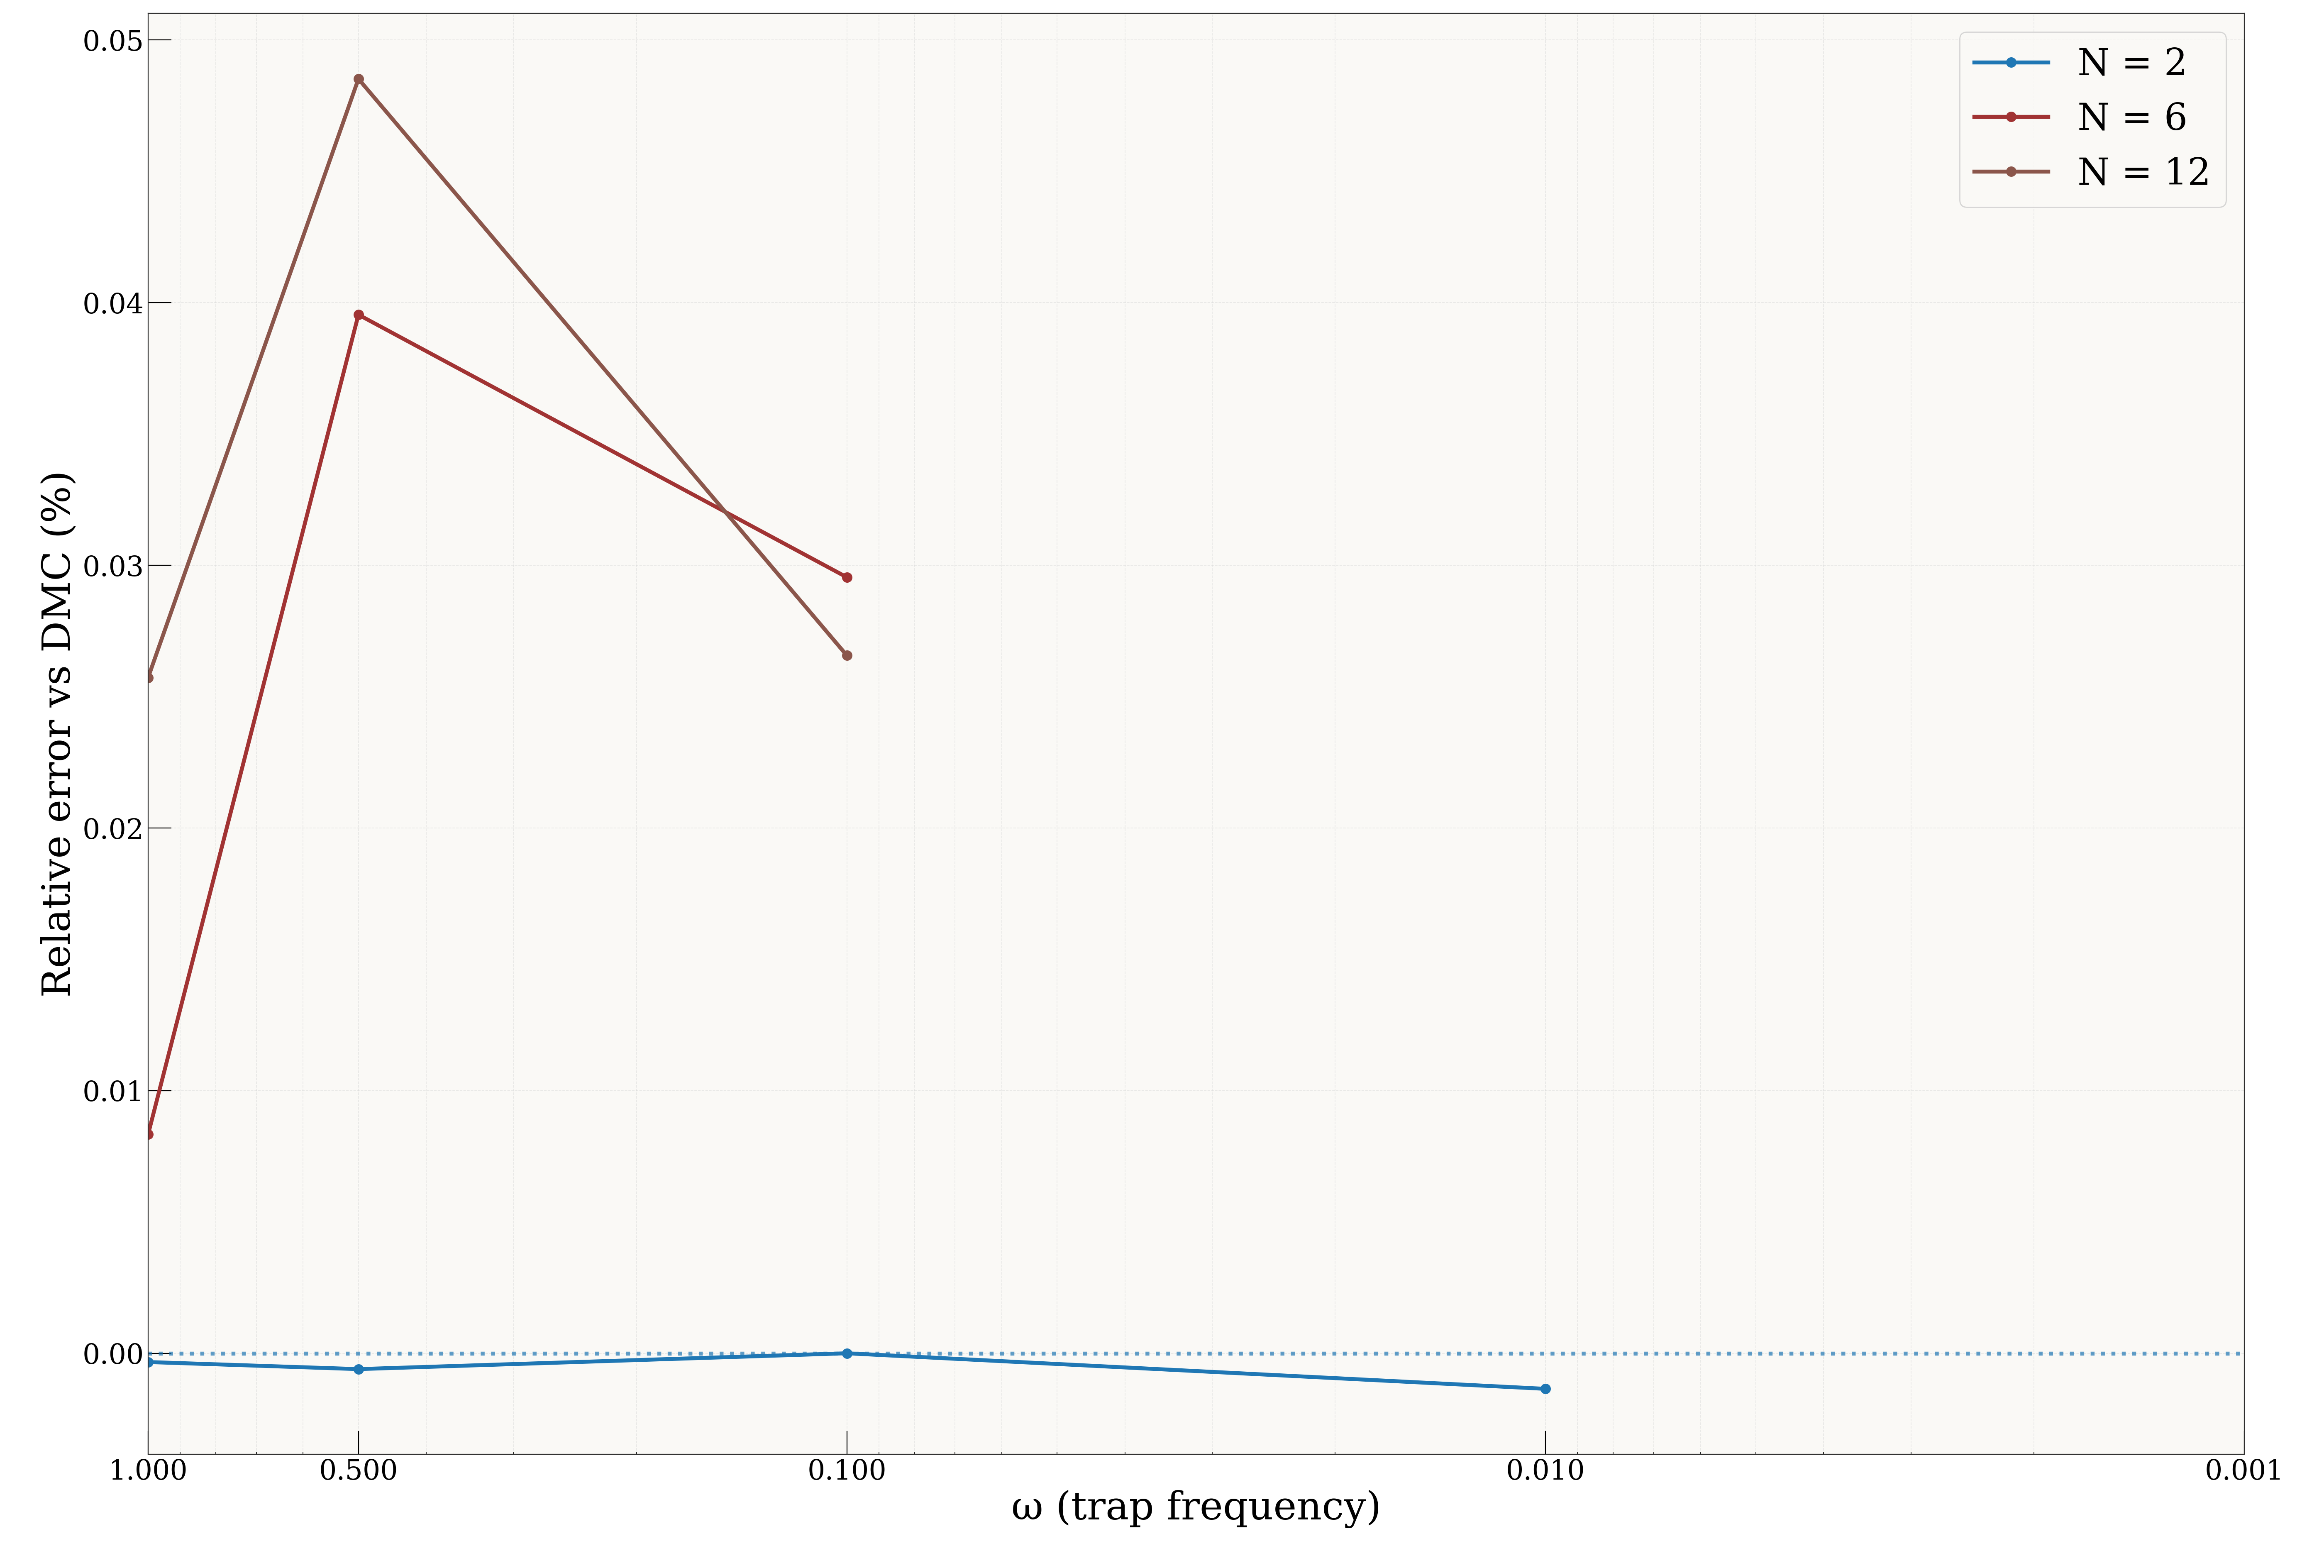
\includegraphics[width=0.9\textwidth]{rel_error_vs_omega_allN}
  \caption[Relative deviation from the external references]{Relative deviation of the conv.-BF
  energies from the external references (Table~\ref{tab:energies}) at every $(N,\omega)$
  where one exists: fixed-node DMC~\cite{Hogberget2013-DMC} for $N{=}6$ and $12$, and the
  compiled DMC and analytic~\cite{Taut1994-TwoElectrons} values for $N{=}2$. Deviations are at
  the $10^{-3}\,\%$ level for $N{=}2$, comparable to the reference's own precision, and
  $0.008$--$0.05\,\%$ for $N{=}6$ and $12$, with no trend in $\omega$.}
  \label{fig:rel_error_vs_omega}
\end{figure}

\FloatBarrier
\paragraph{The same benchmark, without a Markov chain.}
Everything above was trained with a Markov chain: residual pretraining, then an SR tail
that draws its samples from $|\Psi|^2$ by Metropolis. A second route removes the chain from
the gradient entirely, replacing it with an analytic proposal and importance weights. It
reaches comparable energies over part of this range. Its performance, its failure boundary
and the mechanism behind both are the subject of \S\ref{sec:kernel-mcmcfree}, and the
energies are tabulated there (Table~\ref{tab:collocation}) and not here, because they
are not interpretable until that mechanism is in hand.

\paragraph{Where the tables stop.}
One subtlety matters here, because the MP-BF ansatz sits \emph{below} the quoted DMC
reference in four cells, and at $N{=}12$ and $N{=}20$, $\omega=1$, by more than ten combined
standard errors (for example $65.6956$ vs.\ $65.7001$\,Ha at $N{=}12$). This does not violate
the variational principle, which bounds the energy from below only by the \emph{exact}
ground state, $E_{\rm VMC}\ge E_0$; the DMC benchmarks are \emph{fixed-node} calculations
and carry their own nodal bias. A better nodal surface in the network would produce exactly
this pattern. It is not the only thing that would, but one alternative can be set aside. A
difference in the convention for the Hamiltonian or its units is ruled out: the same ansatz
reproduces the exact two-electron value $3.00000$ at $\omega=1$, and a convention mismatch
would shift every cell, not four. What remains is a time-step or population extrapolation in
the reference, an underestimated statistical error on either side, or an error somewhere in
the chain of compilations by which the reference reached us (see the notes to
Table~\ref{tab:energies}), and nothing here distinguishes these from better nodes. The clean test is a fixed-node DMC
calculation that uses the network's own nodes as its trial surface, which we have not run.
The sub-reference values are therefore recorded as deviations and not interpreted.

Wherever an external check exists, the pattern is the same. For $N{=}2$ the ansatz reaches reference
accuracy at every $\omega$ at which it is compared with one, and for $N\!\in\!\{6,12\}$
the relative deviation stays within $0.008$–$0.05\%$ across the benchmarked
range ($\omega\ge0.1$; Fig.~\ref{fig:rel_error_vs_omega}). Below $\omega=0.1$ there
is no DMC reference for $N\ge6$, and we make no claim of absolute accuracy there;
what we can say is that the energies join smoothly onto the benchmarked regime and, in
the deep-Wigner limit, follow a power law whose fitted exponent, $0.689$ for $N{=}6$
(\S\ref{sec:kernel-q3-frontier}), sits close to the classical Wigner value $2/3$. The efficiency is as notable as the accuracy: the SR
tail converges in $10^3$–$3\times10^3$ iterations of $\sim 3{\times}10^3$ samples
each, a modest optimisation budget for a fully many-body wavefunction. We attribute
this stability to a small set of conditioning choices---
trap-unit scaling, soft-core pair features with $ds/dr\!\to\!0$ at coalescence, and
an explicit analytic cusp---each of which keeps the gradients and the Laplacian
numerically tame from the shallowest trap to the tightest.

\section{Wigner--molecule crossover}
\label{sec:wigner-molecule}

Up to this point the wavefunction has been the thing under examination. Here it becomes
the instrument.

\textbf{The result of this section is that the crossover is staged.} As the trap weakens the
cloud first expands and its shells stiffen \emph{radially}---the width-to-radius ratio
falls, discrete occupancies emerge, the energy partition approaches classical force
balance---while the electrons remain very nearly disordered in angle within those shells.
Angular structure then develops in two steps of its own: a small, gradually growing
correlation that is measurable well before the Wigner regime, and a large
bond-orientational ordering confined to the final decade of confinement. Against the
random-angle baseline the shell bond order runs at $0.99$--$1.01$ of its null value from
$\omega=1$ down to $\omega=0.1$, reaches $1.08$ at $\omega=0.01$ for $N{=}6$ (and stays
within $1.02$ at $N{=}12$ and $N{=}20$), and only at $\omega=10^{-3}$ jumps to $1.16$--$1.63$
on every ring at every particle number. Radial localisation and angular crystallisation are
not one transition, and the diagnostics below are arranged to separate them.

\paragraph{Which states these are.}
Every state in this section is the lowest we find with $N_\uparrow=N_\downarrow$ held fixed,
starting from the closed-shell singlet of the non-interacting problem. That is not a
formality here. Fixing the spin projection does not fix the total spin, since an $S=1$ state
also has an $S_z=0$ component, and we never compare sectors of different $S$. In parabolic
dots the interaction is known to drive spin transitions as it strengthens---for instance
$S=0\!\to\!S=1$ at $N=6$ in the strongly correlated regime~\cite{Egger_1999}---so a change
of ground-state spin is plausible precisely at the weakest traps, where the structural
conclusions below are strongest. The deep-Wigner states are therefore the lowest states
found within a fixed spin-projection sector, not established global ground states, and
every statement below is about them. There is a reason to expect the \emph{charge}
geometry to be less sensitive than the energy ordering---deep in the Wigner regime exchange
is weak and states of different $S$ become nearly degenerate over the same classical
arrangement---but that is an expectation we have not tested, not a result.

The subsections take that in order. \S\ref{sec:wigner-onebody} shows the cloud expanding and
acquiring visible radial structure; \S\ref{sec:wigner-energy} shows interactions taking over
and the trap--interaction partition approaching its classical form;
\S\ref{sec:wigner-radial} shows the shells stiffening radially; and
\S\ref{sec:wigner-angular} shows angular order finally appearing, tested against a null in
which the angles are random. \S\ref{sec:wigner-synthesis} collects what the diagnostics
agree on and what they do not establish.

What we are looking for cannot be seen in the observable one would naturally plot. In a
rotationally symmetric trap, the electrons of a Wigner molecule localise in \emph{relative} coordinates (concentric rings, polygon-like angular correlations) while the whole pattern is free to rotate. Average over that rotation, as
any lab-frame density does, and the rings smear into something close to uniform. The
order is there; the density hides it. Every diagnostic below exists to look past that
averaging.

We combine one-body densities, label-invariant shell topology, rotation-registered
angular order, shell radii and gaps, pair statistics, and Lindemann-type disorder, across
$N=2,6,12,20$ and $\omega\in\{1,0.5,0.1,0.01,0.001\}$~\cite{Egger_1999,manninen2007metalclustersquantumdots}.
No one of them is decisive on its own. They fail in different ways, which is why they are
reported together.

% ──────────────────────────────────────────────────────────────────────
\subsection{Observables and diagnostics}
\label{sec:wigner-diagnostics}

For each $(N,\omega)$ we draw $\mathbf X\!\sim|\Psi|^2$ and report
(i)~the pair distribution $g(r)$,
(ii)~the single-particle radial density $P(r)\!\propto\!r\,\rho(r)$,
and summary statistics: $r_{\rm mode}$, $\langle r\rangle$, $\sigma_r$, FWHM,
quantiles $q_{10},q_{50},q_{90}$, and a localisation ratio
$\gamma=\sigma_r/r_{\rm mode}$ (smaller $\gamma$ $\Rightarrow$ stiffer
localisation).
For multi-electron systems we additionally monitor shell-resolved
bond-orientational order $|\Phi_m|$ and a dimensionless Lindemann-type
ratio for positional fluctuations on each
ring~\cite{Mazars_2008}.

\paragraph{Density parameter $r_s$.}
Following Egger \textit{et al.}~\cite{Egger_1999}, we estimate the Wigner--Seitz
parameter from the first maximum $r^\ast$ of the spin-summed pair correlation,
$r_s\equiv r^\ast/a_B^\ast$.
The Fermi--liquid $\to$ Wigner--molecule crossover occurs near $r_s\!\simeq\!4$
in parabolic dots; our weak-trap cases lie well beyond this
threshold~\cite{Egger_1999,Filinov_2001}.

% ──────────────────────────────────────────────────────────────────────
\subsection{One-body densities: visual crossover}
\label{sec:wigner-onebody}

Figures~\ref{fig:onebody_grid} and~\ref{fig:onebody_n20} compare one-body
densities at strong confinement ($\omega=1$) and weak confinement
($\omega=10^{-3}$) for $N=2,6,12,20$.
At $\omega=1$ the density remains compact and the dominant change with $N$ is
progressive shell filling under the harmonic trap. At $\omega=10^{-3}$ it broadens by two
orders of magnitude and develops pronounced \emph{radial} structure at every $N$.

What that structure can and cannot establish follows from the symmetry argument above. The
lab-frame density is an average over all orientations of the molecule, so it retains radial
information and destroys angular information by construction. These figures are therefore
evidence of \emph{radial shell localisation} and are silent on whether the electrons are
angularly ordered within those shells---a ring of six electrons at fixed $60^\circ$ spacing
and six electrons sliding freely around the same ring produce the same picture. The angular
question is taken up in \S\ref{sec:wigner-angular}, where it needs a co-rotating frame and a
null model to answer.

\begin{figure*}[htbp]
  \centering
  \captionsetup[subfigure]{justification=centering,font=small}

  % ---------- Row 1: ω = 1.0 ----------
  \begin{subfigure}[t]{\threecolw}
    \centering
    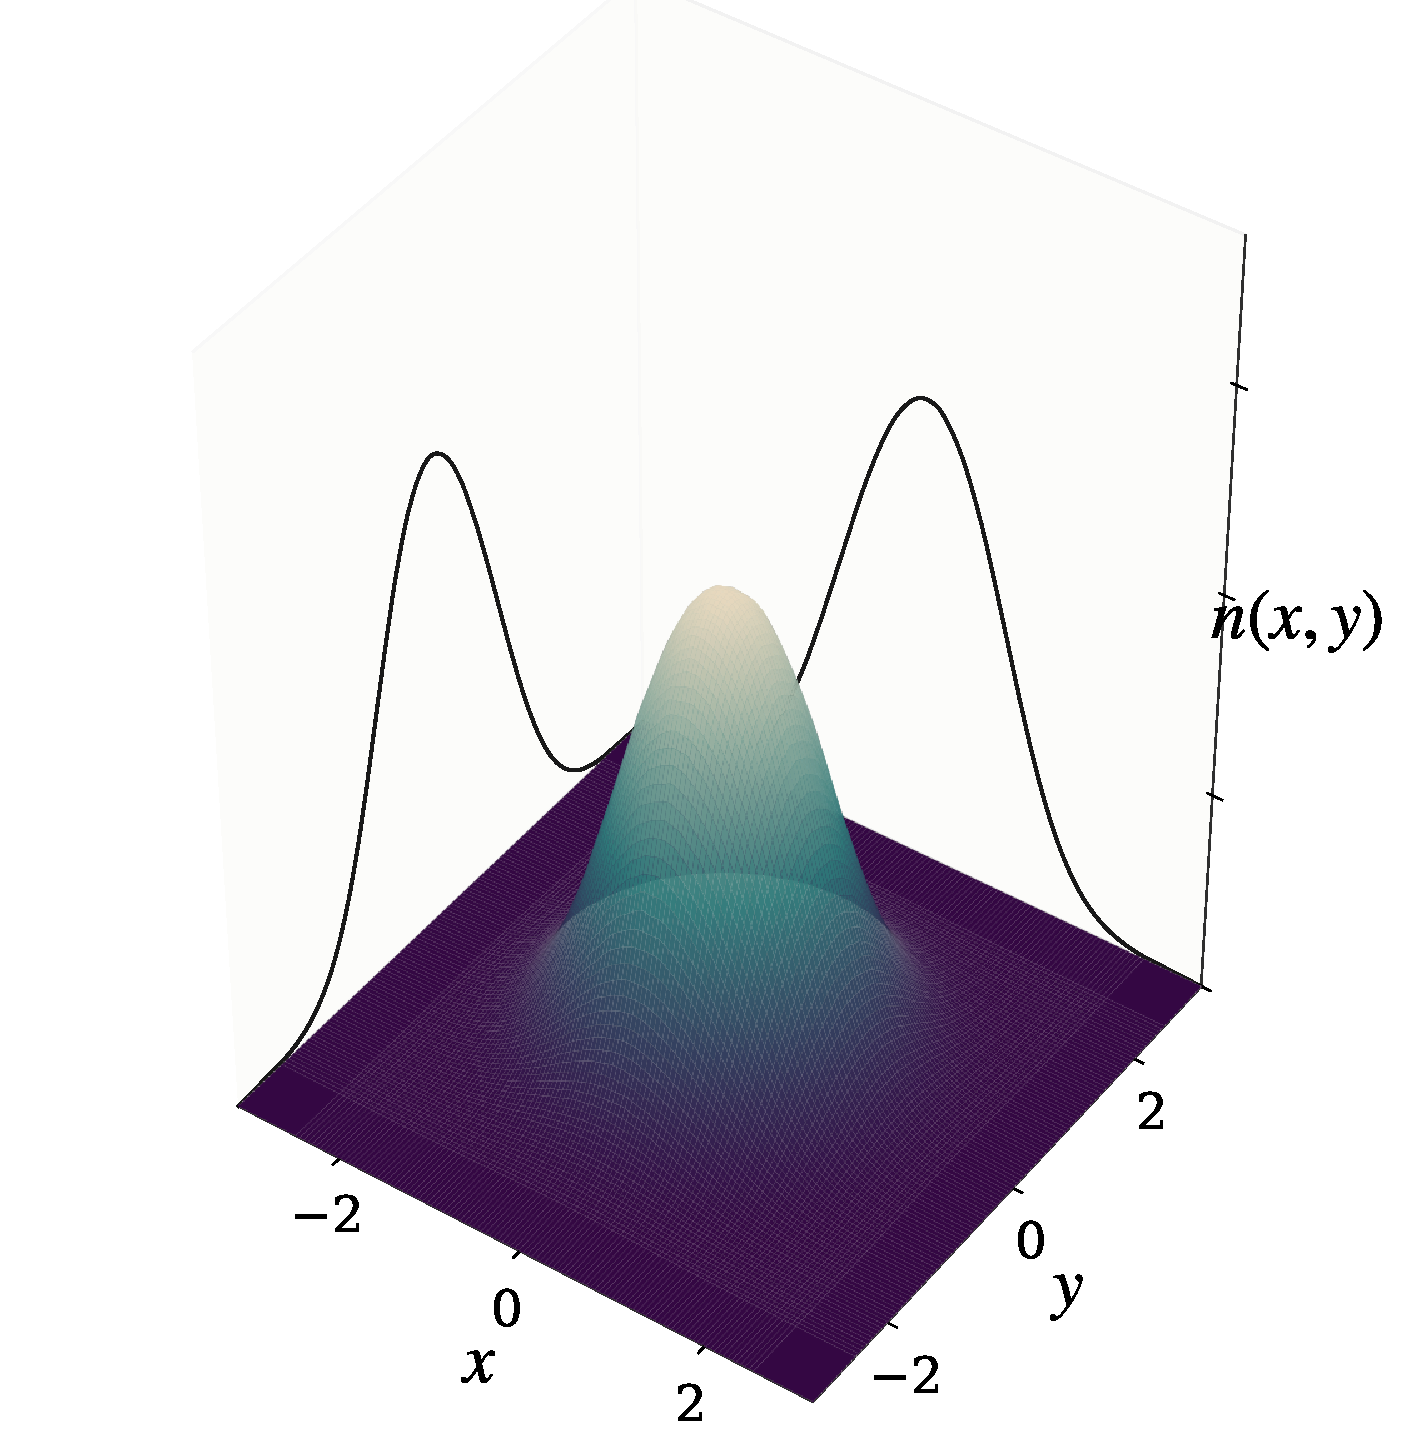
\includegraphics[width=\linewidth]{one_body_density_2_omega_1.00000_20251029_231309.pdf}
    \caption{$N{=}2,\;\omega=1.0$}
  \end{subfigure}\hspace{\figgutter}%
  \begin{subfigure}[t]{\threecolw}
    \centering
    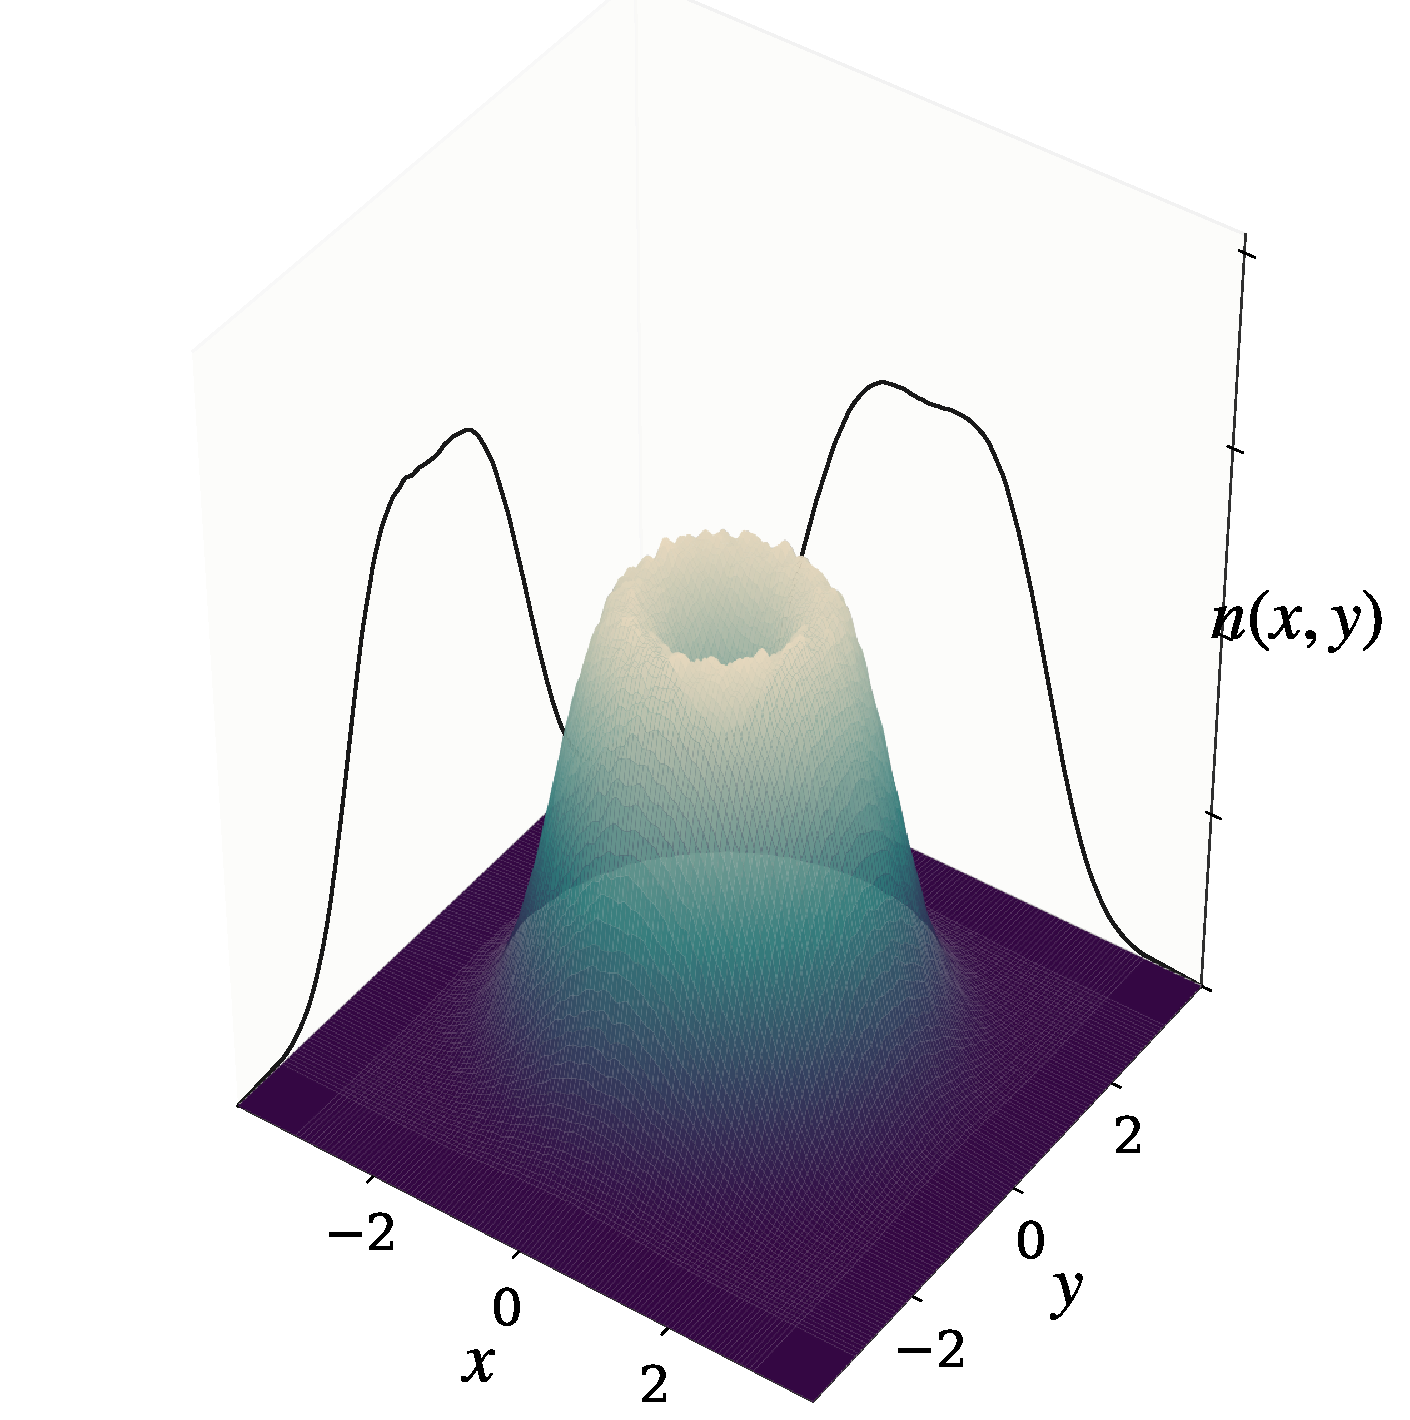
\includegraphics[width=\linewidth]{one_body_density_6_omega_1.00000_20251030_093439.pdf}
    \caption{$N{=}6,\;\omega=1.0$}
  \end{subfigure}\hspace{\figgutter}%
  \begin{subfigure}[t]{\threecolw}
    \centering
    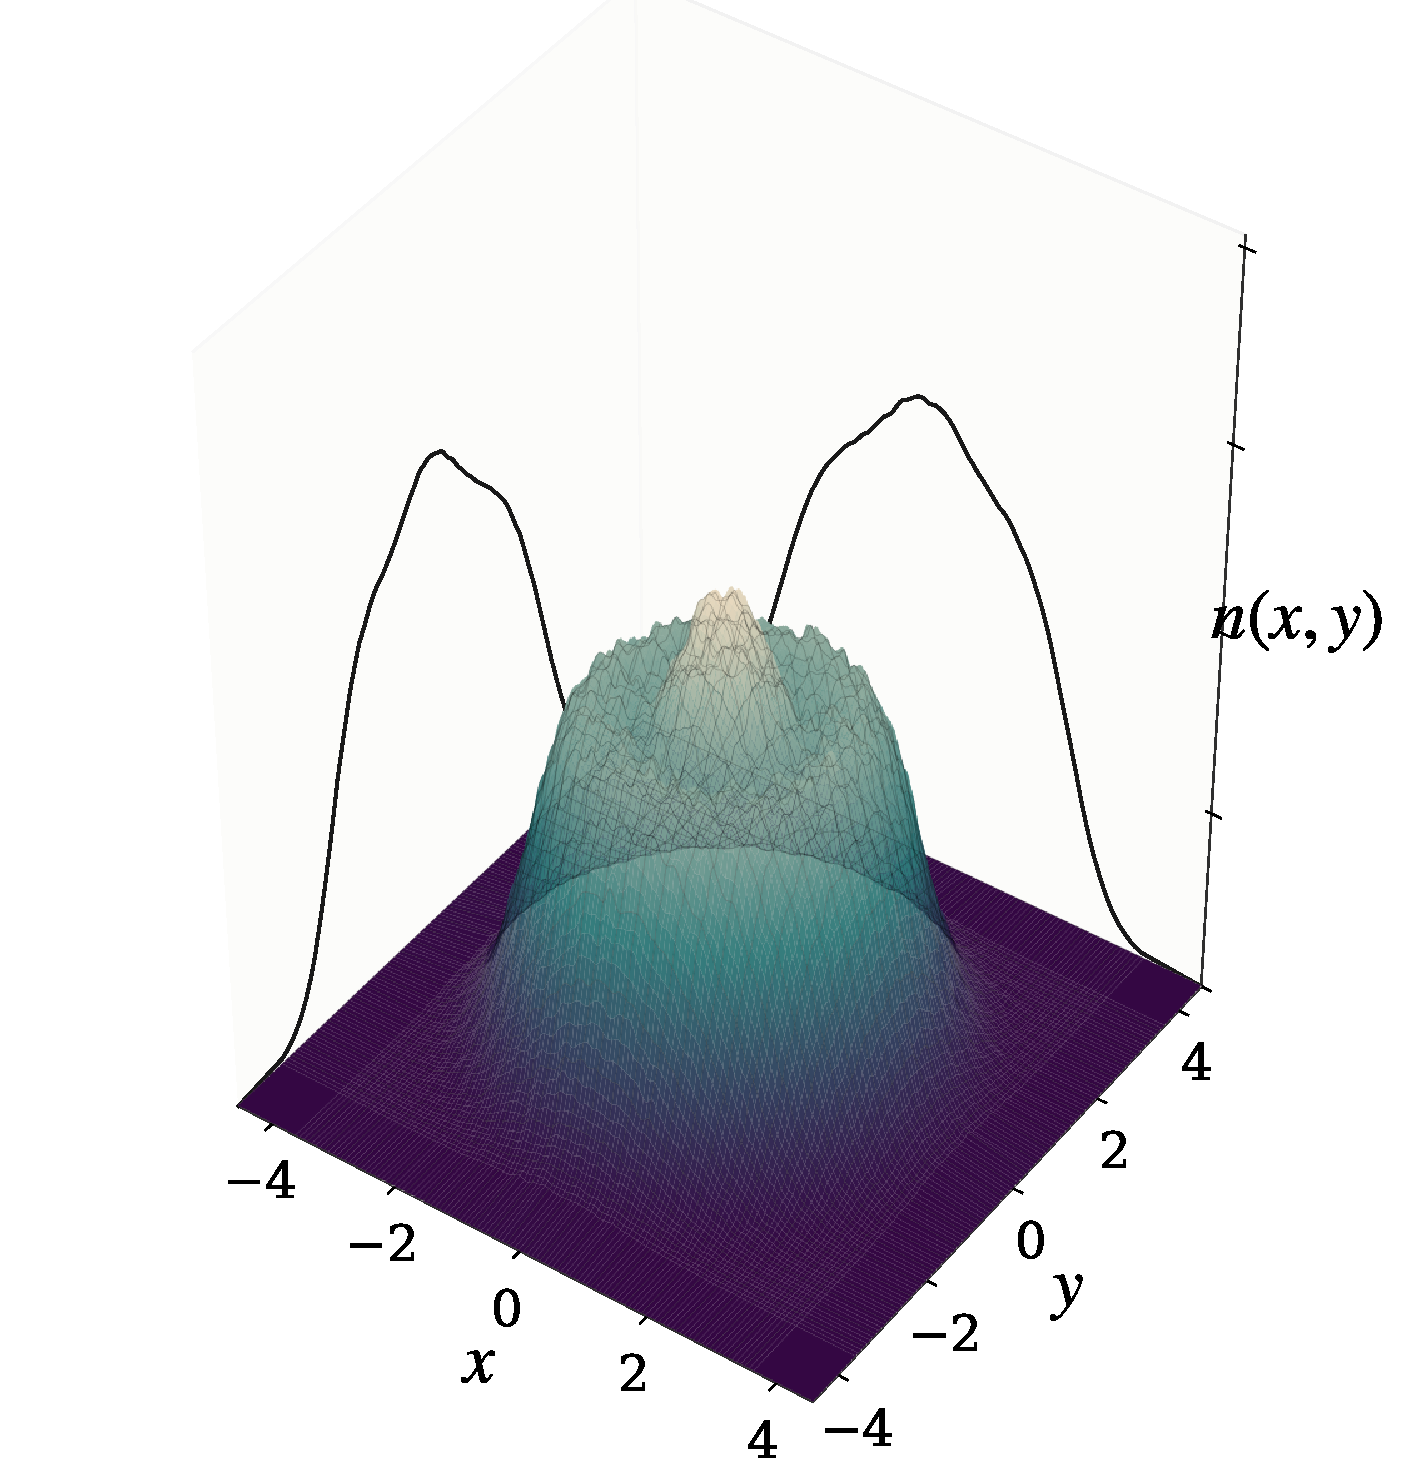
\includegraphics[width=\linewidth]{one_body_density_12_omega_1.00000_20251104_194000.pdf}
    \caption{$N{=}12,\;\omega=1.0$}
  \end{subfigure}

  \vspace{0.5em}

  % ---------- Row 2: ω = 0.001 ----------
  \begin{subfigure}[t]{\threecolw}
    \centering
    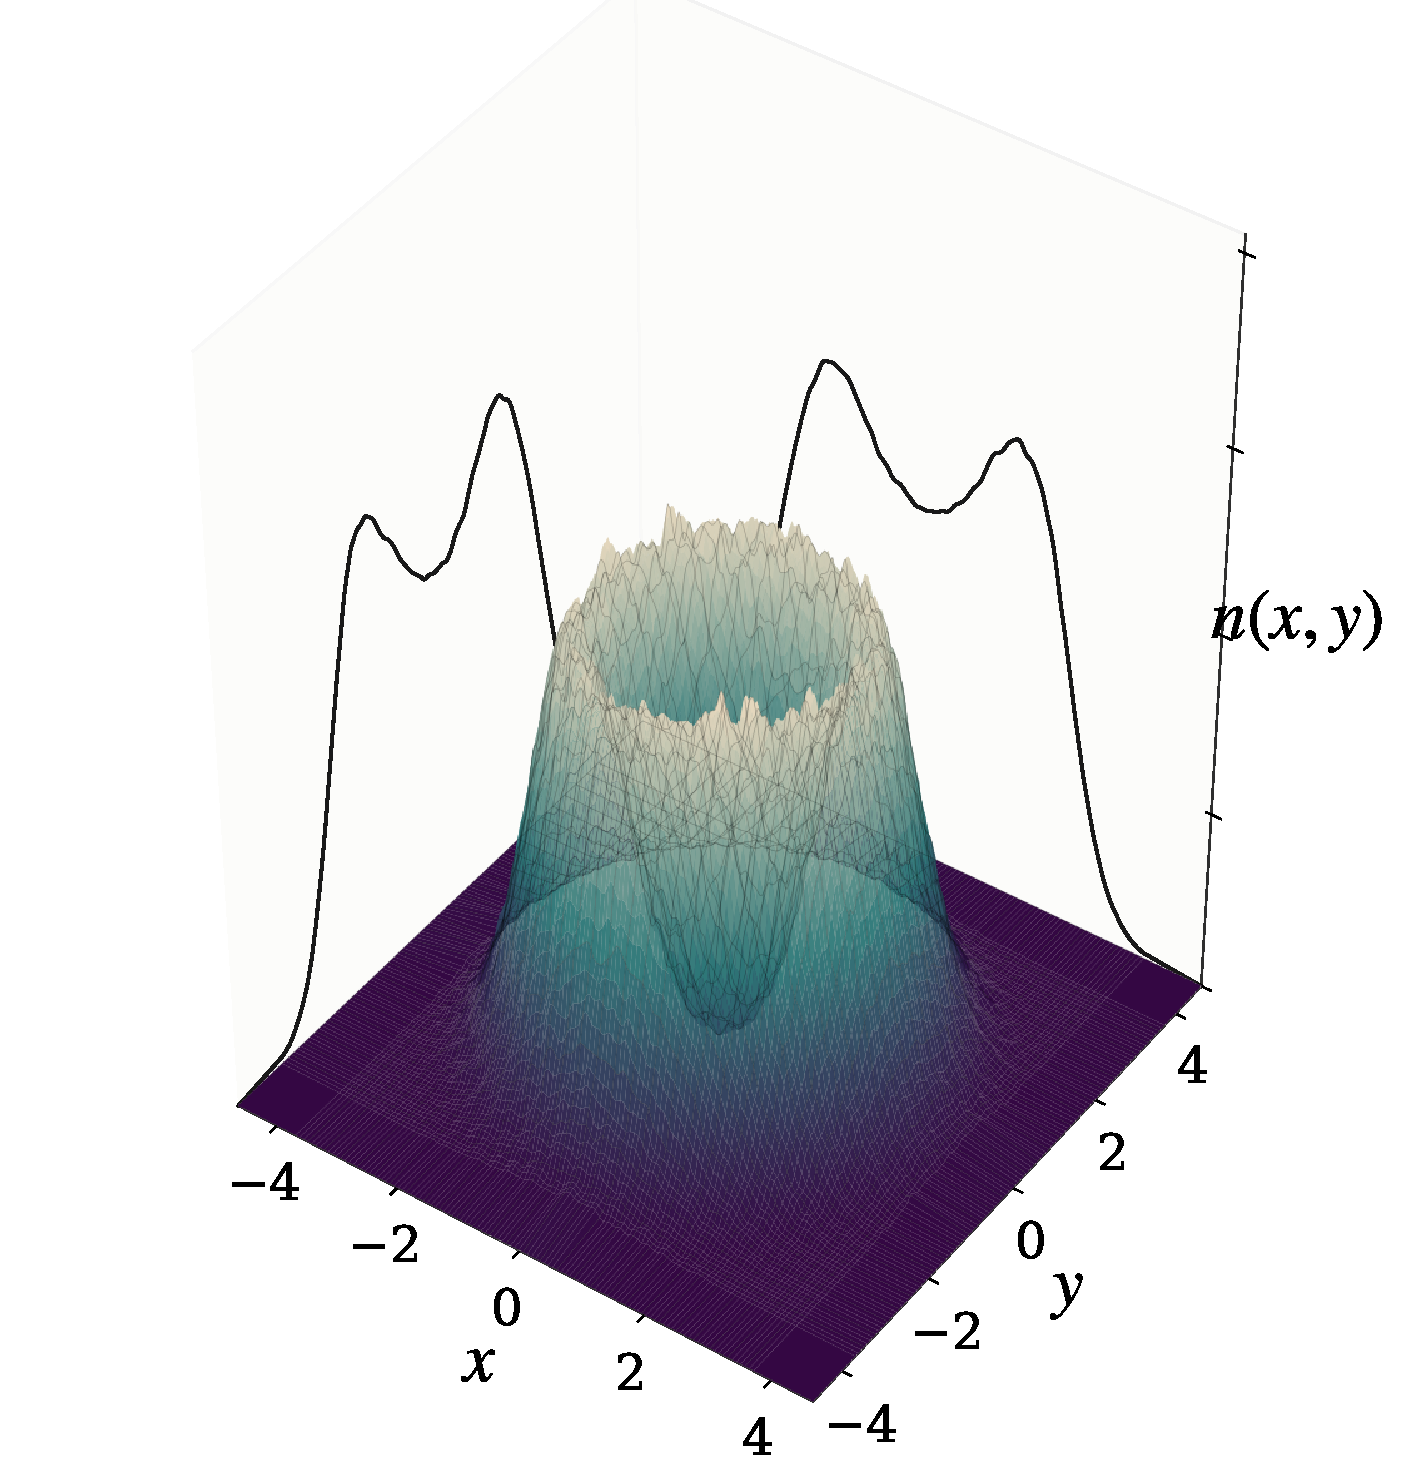
\includegraphics[width=\linewidth]{one_body_density_2_omega_0.00100_20251106_160757.pdf}
    \caption{$N{=}2,\;\omega=0.001$}
  \end{subfigure}\hspace{\figgutter}%
  \begin{subfigure}[t]{\threecolw}
    \centering
    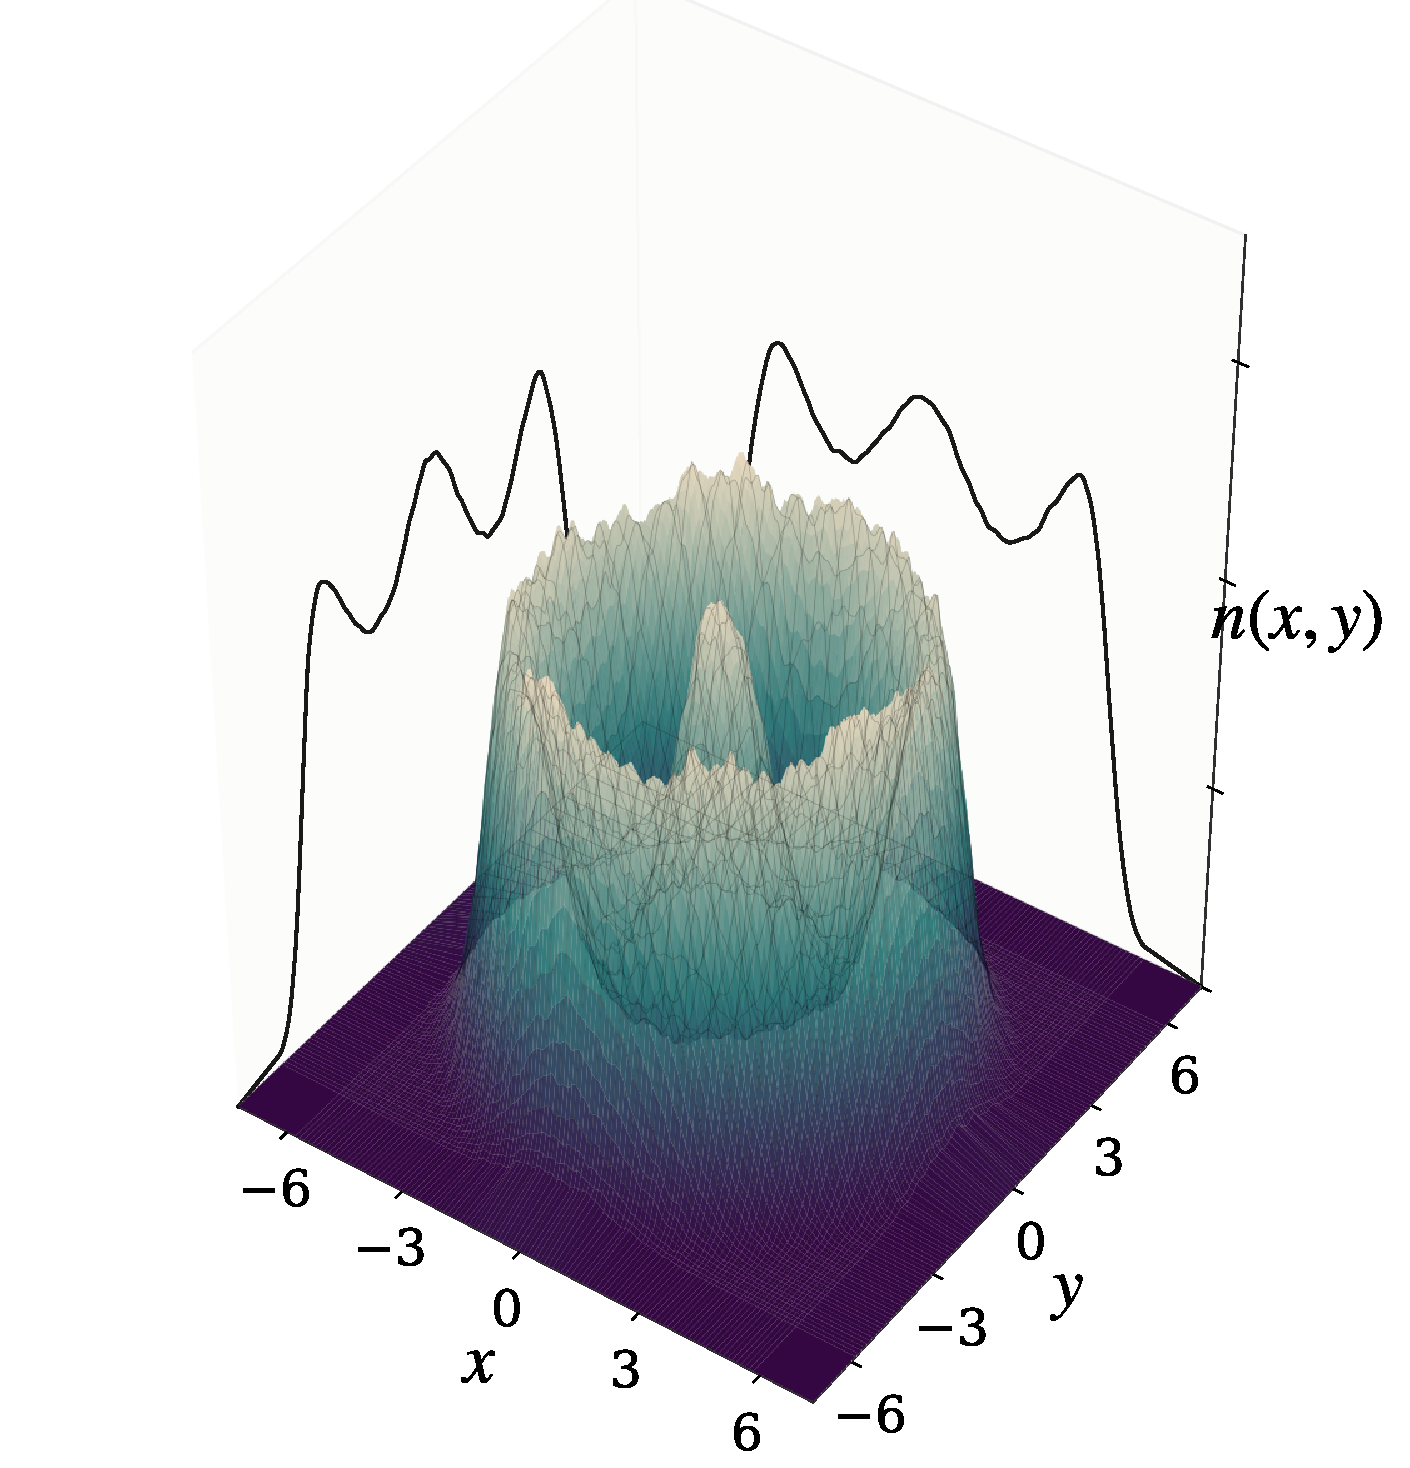
\includegraphics[width=\linewidth]{one_body_density_6_omega_0.00100_20251106_214930.pdf}
    \caption{$N{=}6,\;\omega=0.001$}
  \end{subfigure}\hspace{\figgutter}%
  \begin{subfigure}[t]{\threecolw}
    \centering
    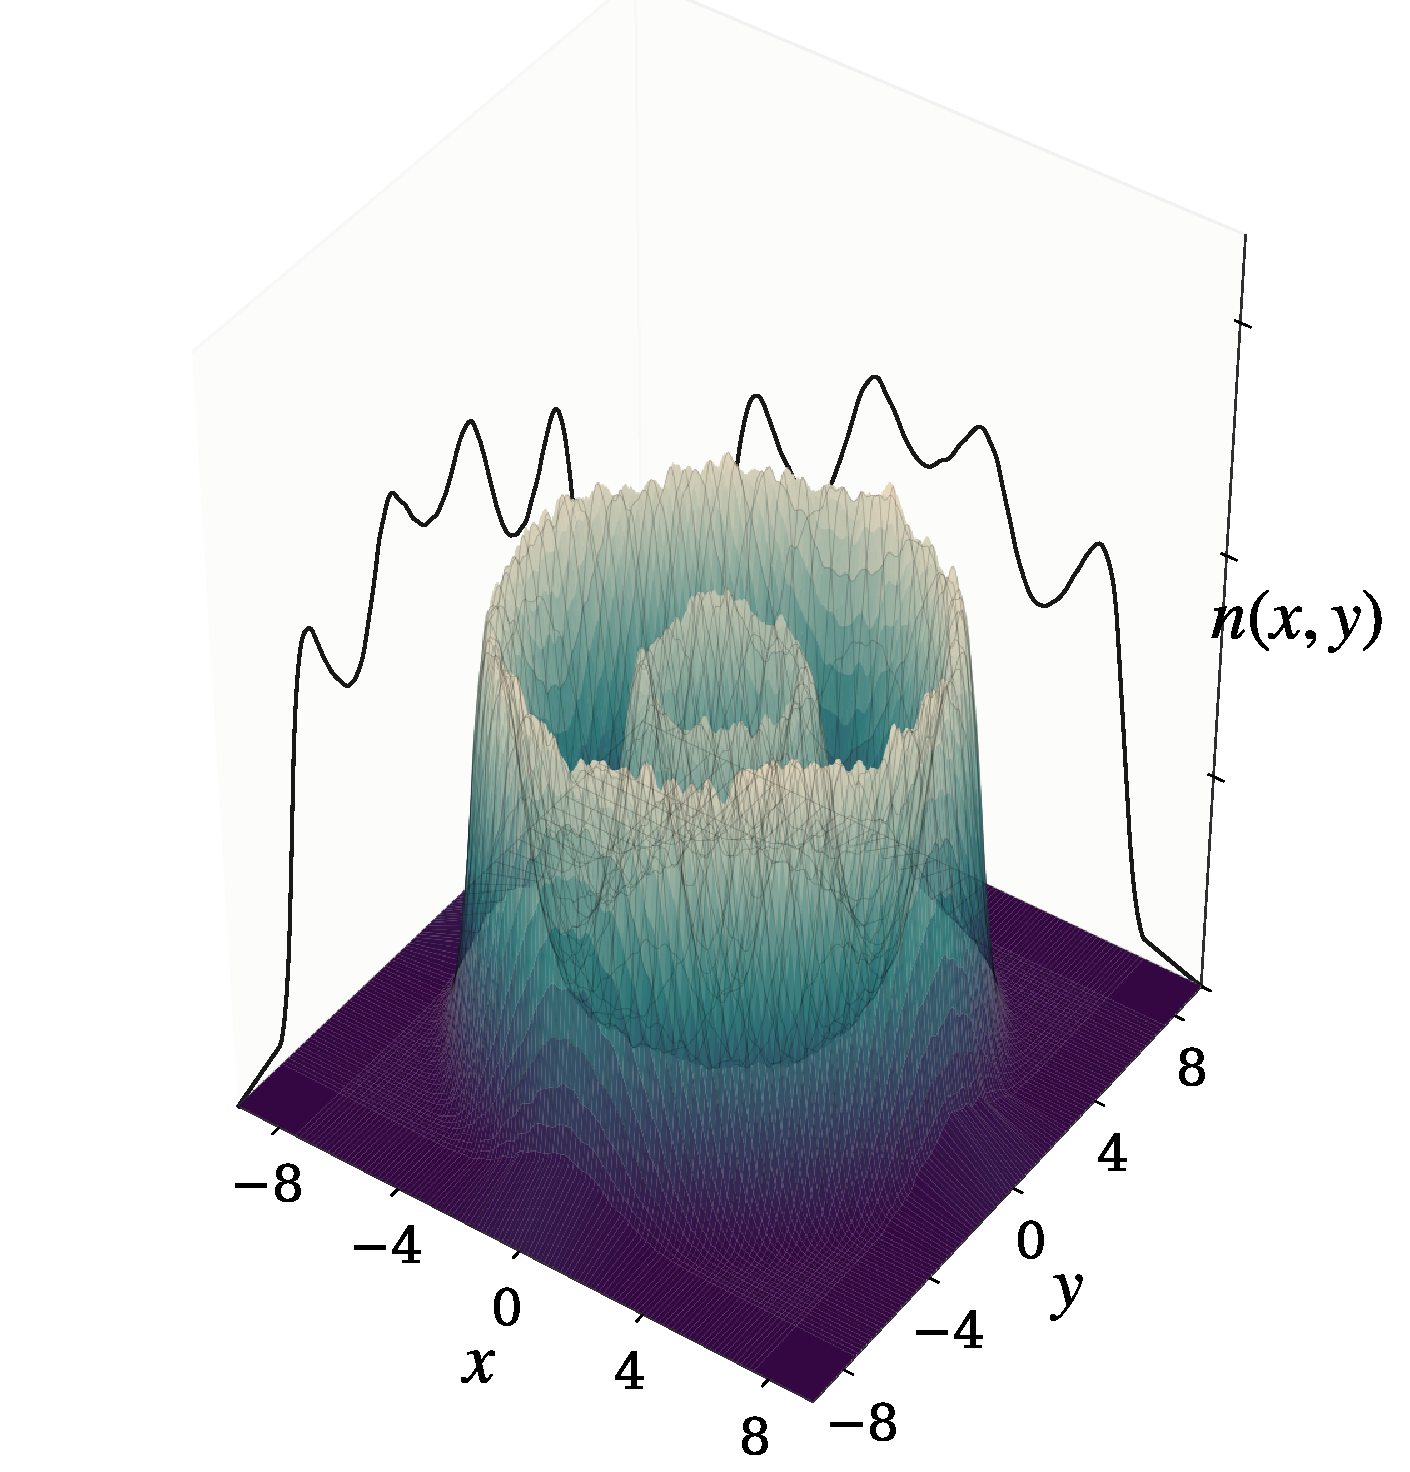
\includegraphics[width=\linewidth]{one_body_density_12_omega_0.00100_20251109_110913.pdf}
    \caption{$N{=}12,\;\omega=0.001$}
  \end{subfigure}

  \caption[One-body densities at strong and weak confinement, $N=2,6,12$]{One-body
  densities for $N=2,6,12$ at $\omega=1.0$ (top) and $\omega=0.001$ (bottom). The vertical
  axis is the one-body density $n(x,y)$ over the two Cartesian components of a single
  particle's position, in trap units; the curves on the back walls are its marginals. As
  confinement weakens the densities broaden
  and develop pronounced \emph{radial} shell structure. Being lab-frame averages over all
  orientations of the molecule, they cannot show angular order: that requires the registered
  diagnostics of \S\ref{sec:wigner-angular}.}
  \label{fig:onebody_grid}
\end{figure*}

\begin{figure}[htbp]
  \centering
  \captionsetup[subfigure]{justification=centering,font=small}
  \begin{subfigure}[t]{0.48\textwidth}
    \centering
    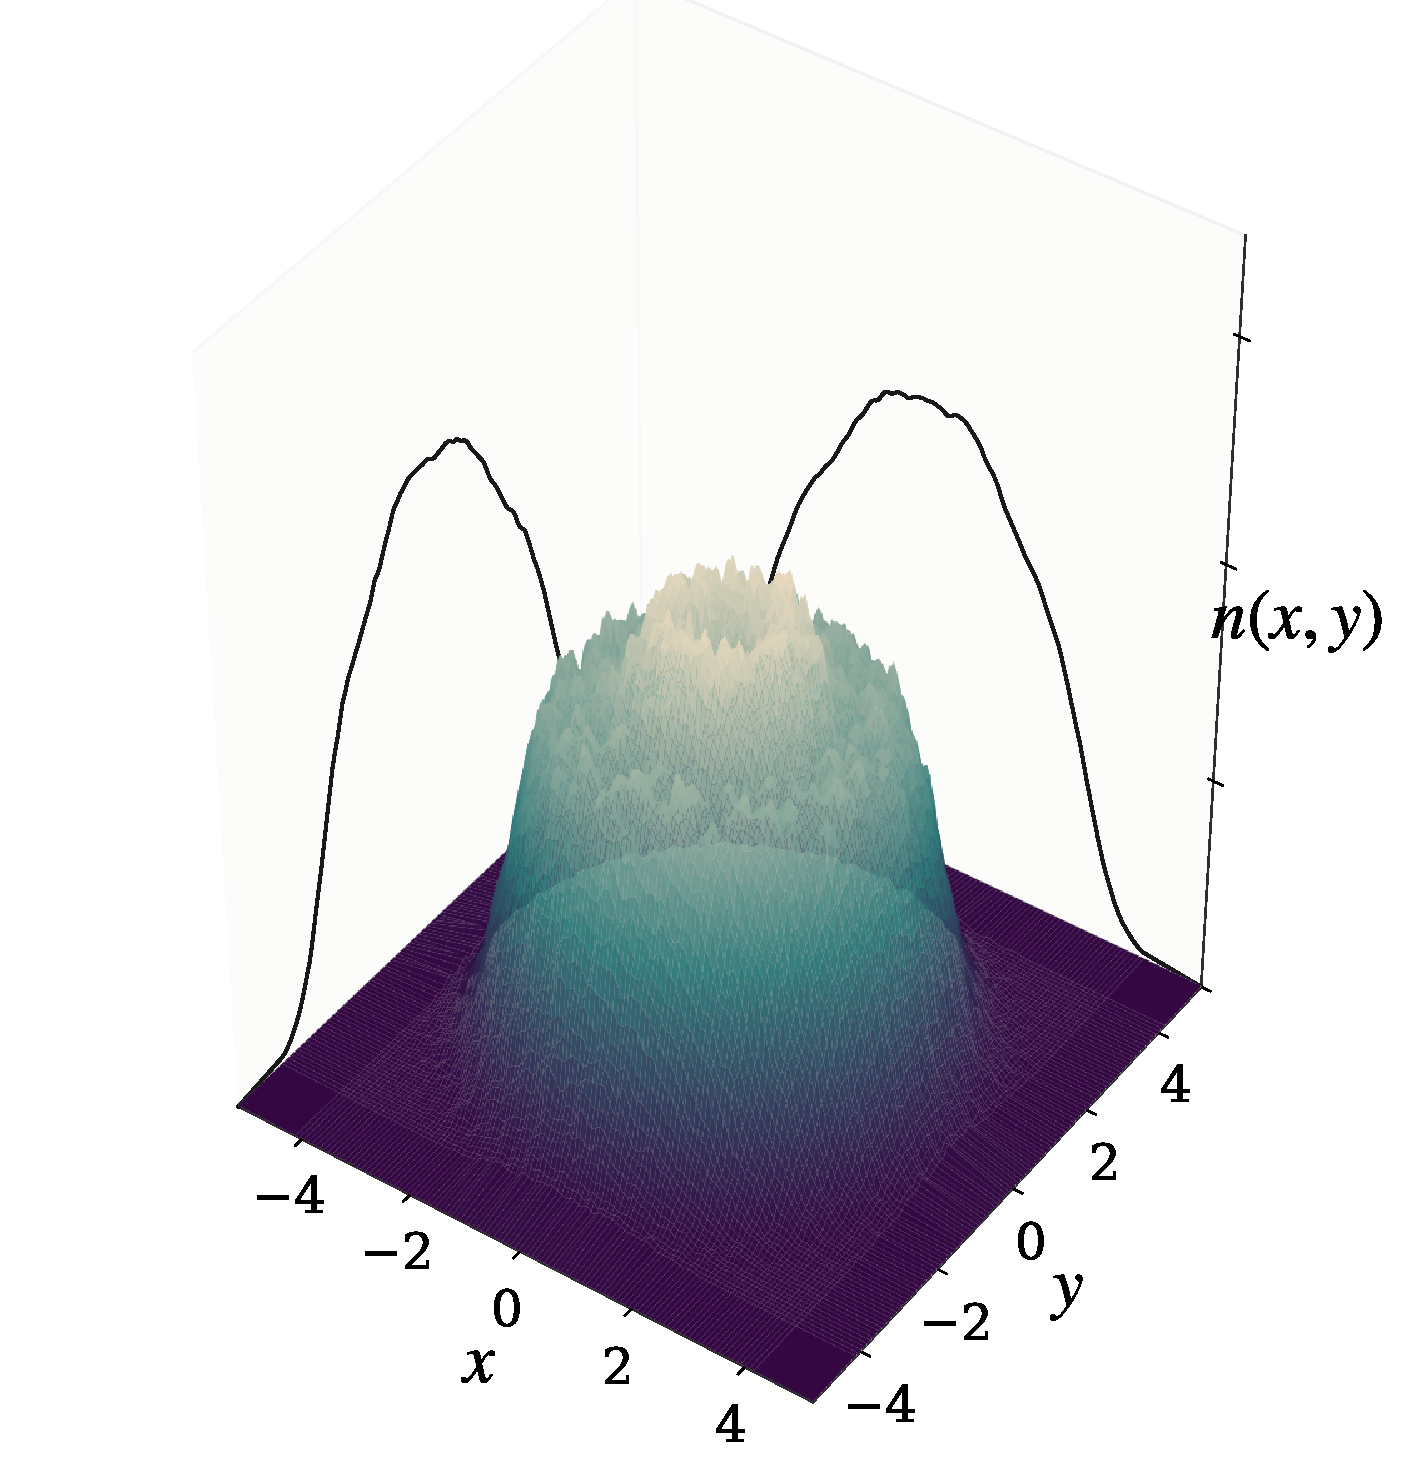
\includegraphics[width=\linewidth]{one_body_density_20_omega_1.00000_20251228_180301.pdf}
    \caption{$N{=}20,\;\omega=1.0$}
  \end{subfigure}
  \hfill
  \begin{subfigure}[t]{0.48\textwidth}
    \centering
    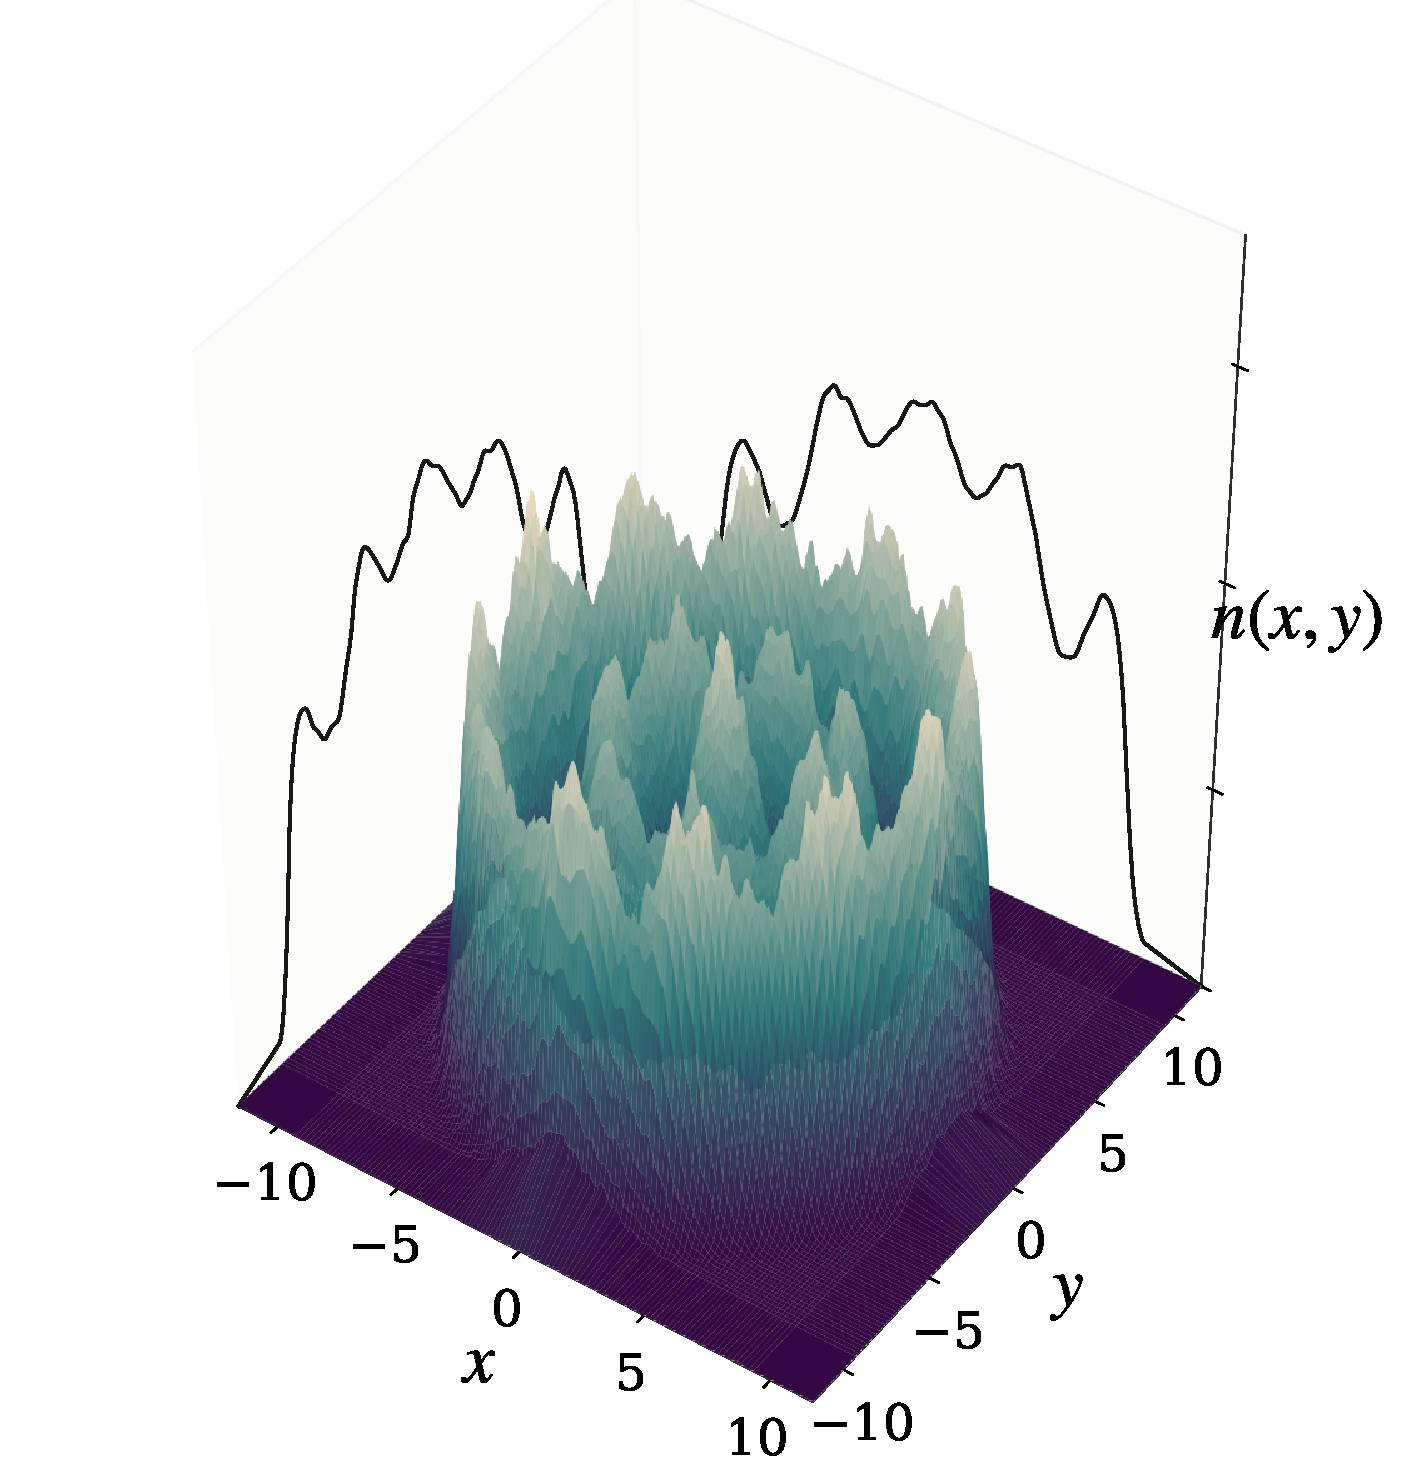
\includegraphics[width=\linewidth]{one_body_density_20_omega_0.00100.pdf}
    \caption{$N{=}20,\;\omega=0.001$}
  \end{subfigure}
  \caption[One-body densities at strong and weak confinement, $N{=}20$]{One-body densities
  for $N{=}20$ at strong and weak confinement; the vertical axis is $n(x,y)$ as in
  Fig.~\ref{fig:onebody_grid}. The weak-trap case shows strong radial broadening and clear
  multi-shell organisation. As above, this is radial evidence only.}
  \label{fig:onebody_n20}
\end{figure}

% ──────────────────────────────────────────────────────────────────────
\subsection{Energy-based crossover diagnostics}
\label{sec:wigner-energy}

\begin{figure*}[htbp]
  \centering
  \captionsetup[subfigure]{justification=centering}

  \begin{subfigure}[t]{0.48\textwidth}
    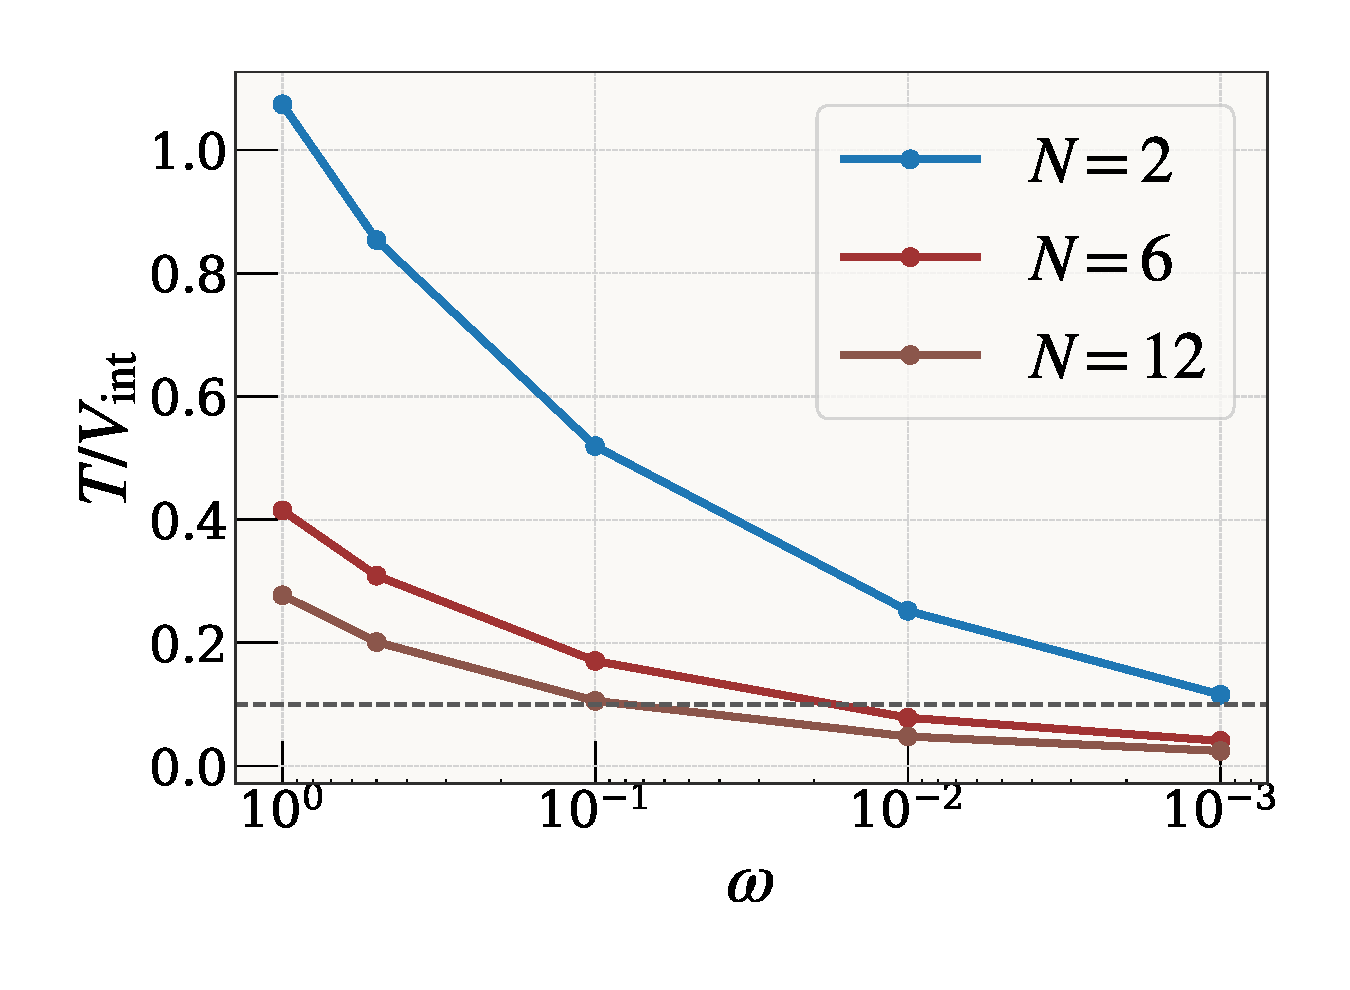
\includegraphics[width=\linewidth]{ratio_T_over_Vint_desc_allN}
    \caption[]{$T/V_{\rm int}$ vs.\ $\omega$ for $N{=}2,6,12$.
    The horizontal line marks $T/V_{\rm int}{=}0.1$.}
  \end{subfigure}
  \hfill
  \begin{subfigure}[t]{0.48\textwidth}
    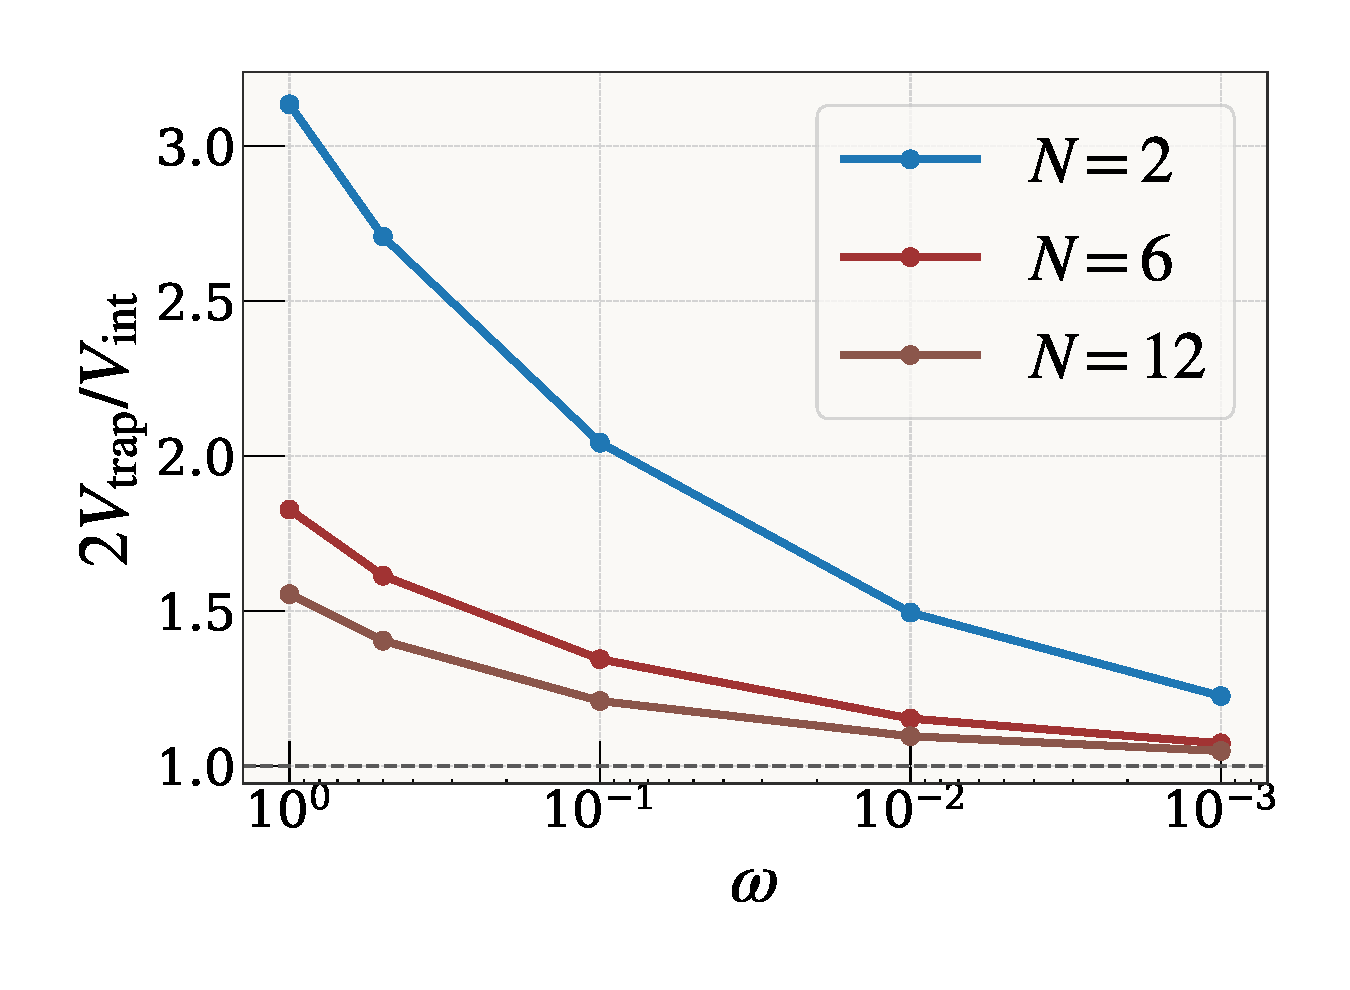
\includegraphics[width=\linewidth]{ratio_2Vtrap_over_Vint_desc_allN}
    \caption[]{$2V_{\rm trap}/V_{\rm int}$ vs.\ $\omega$ for $N{=}2,6,12$.
    The horizontal line marks the classical virial ratio $2V_{\rm trap}=V_{\rm int}$.}
  \end{subfigure}

  \caption[Energy-based Wigner diagnostics against trap frequency]{Energy-based Wigner diagnostics as functions of trap frequency.
  As $\omega$ decreases the dots become interaction dominated
  ($T/V_{\rm int}\!\ll1$) and the trap--interaction partition approaches the
  classical virial form, most clearly for $N{=}12$.}
  \label{fig:wigner_ratios}
\end{figure*}

The energy partition carries two messages, and only two.

\emph{Interactions take over.} The interaction-to-kinetic ratio
$\Gamma=\langle V_{\rm int}\rangle/\langle T\rangle$ rises across
$\omega\in[1,10^{-3}]$ from $0.9$ to $8.6$ at $N{=}2$, from $2.4$ to $24.5$ at $N{=}6$ and
from $3.6$ to $41.1$ at $N{=}12$ (Fig.~\ref{fig:wigner_ratios}a). The dot stops being a
kinetic-energy-dominated droplet and becomes a Coulomb-dominated one.

\emph{Classical force balance emerges.} At $\omega=10^{-3}$ the trap--interaction partition
$2\langle V_{\rm trap}\rangle/\langle V_{\rm int}\rangle$ reaches $1.23$, $1.07$ and $1.05$
at $N=2,6,12$, so the twelve-electron dot satisfies the classical condition
$V_{\rm int}\approx2V_{\rm trap}$ to within $5\%$ (Fig.~\ref{fig:wigner_ratios}b). The
approach is monotone and improves with $N$, as it should: the classical limit is reached
faster when there are more particles to arrange.

Both are consistent with real-space expansion. The rms radius extracted from
$V_{\rm trap}=\tfrac12\omega^2\sum_i\langle r_i^2\rangle$ grows from $1.1$--$2.0\,a_B^\ast$
at $\omega=1$ to $70$--$170\,a_B^\ast$ at $\omega=10^{-3}$, faster than the non-interacting
$\omega^{-1/2}$ law, which is interaction-driven swelling. The fitted exponents for the
individual energy components and for the radius, which support these statements without
adding to them, are collected in Appendix~\ref{app:energy-exponents}.

% ──────────────────────────────────────────────────────────────────────
\subsection{Radial localisation and pair correlations}
\label{sec:wigner-radial}

Over the weakest three confinements, the typical one-body radius follows
$r_{\rm mode}\!\sim\!\omega^{\alpha}$ with $\alpha\simeq-0.626$ at $N{=}2$---close to
the classical two-body value $-2/3$, which nothing in the ansatz knows about. At $N{=}2$ the
width-to-scale ratio $\gamma=\sigma_r/r_{\rm mode}$ falls as well, from $0.49$ to $0.29$, so
the pair stiffens rather than merely dilating. At $N{=}6$ the same global ratio barely moves
(Table~\ref{tab:radial-compact}), and radial stiffening there has to be read from quantities
that resolve the shell, not from this one.

\begin{table}[H]
\centering
\caption[Radial localisation across the confinement range]{Radial localisation across the confinement range. $r_{\rm mode}$ is the mode of
the single-particle radial density in Bohr; $\gamma=\sigma_r/r_{\rm mode}$ is the
width-to-scale ratio. Full diagnostics---mean, width, FWHM, quantiles, ring-angle spread
and pair Lindemann ratio---are in Appendix~\ref{app:structural-tables}. The $N{=}6$ values
at $\omega\le0.01$ come from an earlier run than the shell analysis and
Fig.~\ref{fig:6N_radial_densities} (Appendix~\ref{app:reproducibility}).}
\label{tab:radial-compact}
\begin{tabular}{lcccc}
\toprule
 & \multicolumn{2}{c}{$N{=}2$} & \multicolumn{2}{c}{$N{=}6$} \\
\cmidrule(lr){2-3}\cmidrule(lr){4-5}
$\omega$ & $r_{\rm mode}$ & $\gamma$ & $r_{\rm mode}$ & $\gamma$ \\
\midrule
1.00  & $1.44$  & $0.491$ & $2.09$   & $0.442$ \\
0.50  & $2.30$  & $0.437$ & $3.07$   & $0.445$ \\
0.10  & $3.60$  & $0.480$ & $8.17$   & $0.429$ \\
0.01  & $14.19$ & $0.396$ & $33.15$  & $0.420$ \\
0.001 & $64.29$ & $0.287$ & $113.55$ & $0.421$ \\
\bottomrule
\end{tabular}
\end{table}

The exponent is not the sharpest form of this check. Because $r_{\rm mode}$ is the mode of
the \emph{single-particle} radial density, it mixes the central electron of a $(1,5)$
topology with the ring and is not the ring radius. The shell-resolved outer radius is, and
comparing it with the classical Wigner ring $1.334\,\omega^{-2/3}$ tests a prefactor as
well as a power. That ratio falls monotonically---$1.247$, $1.188$, $1.098$, $1.032$,
$1.017$ from $\omega=1$ to $10^{-3}$---so at the weakest trap the quantum ring sits $1.7\%$
outside the classical one, and the fitted exponent on that quantity is $-0.637$ over the
full grid and $-0.650$ over the weakest three confinements
(Appendix~\ref{app:structural-tables:radius}). Nothing in the ansatz, the objective or the
sampler knows the number $1.334$.

The two sizes stiffen differently, and the difference is physical. At $\omega=10^{-3}$
the $N{=}2$ pair sits at separation $r_{12}\!\approx\!122$ with Lindemann ratio
$\gamma_{r_{12}}\!\approx\!0.20$ and a relative angle sharply peaked at $\pi$: a dilute,
anti-aligned dimer. At $N{=}6$ the global $\gamma$ plateaus near $0.42$, and the evidence
for stiffening comes from the shell-resolved and pair quantities instead: the outer ring's
own relative radial width falls from $0.32$ at $\omega=1$ to $0.15$ at $10^{-3}$
(Table~\ref{tab:shell-summary}), and the ring's angular fluctuations and pair Lindemann
ratio fall monotonically. A single-particle width is the weakest of the radial diagnostics:
it mixes the central electron with the ring, and it is the one quantity here that does not
resolve the shell structure it is being asked about.

\begin{figure}[htp]
  \centering
  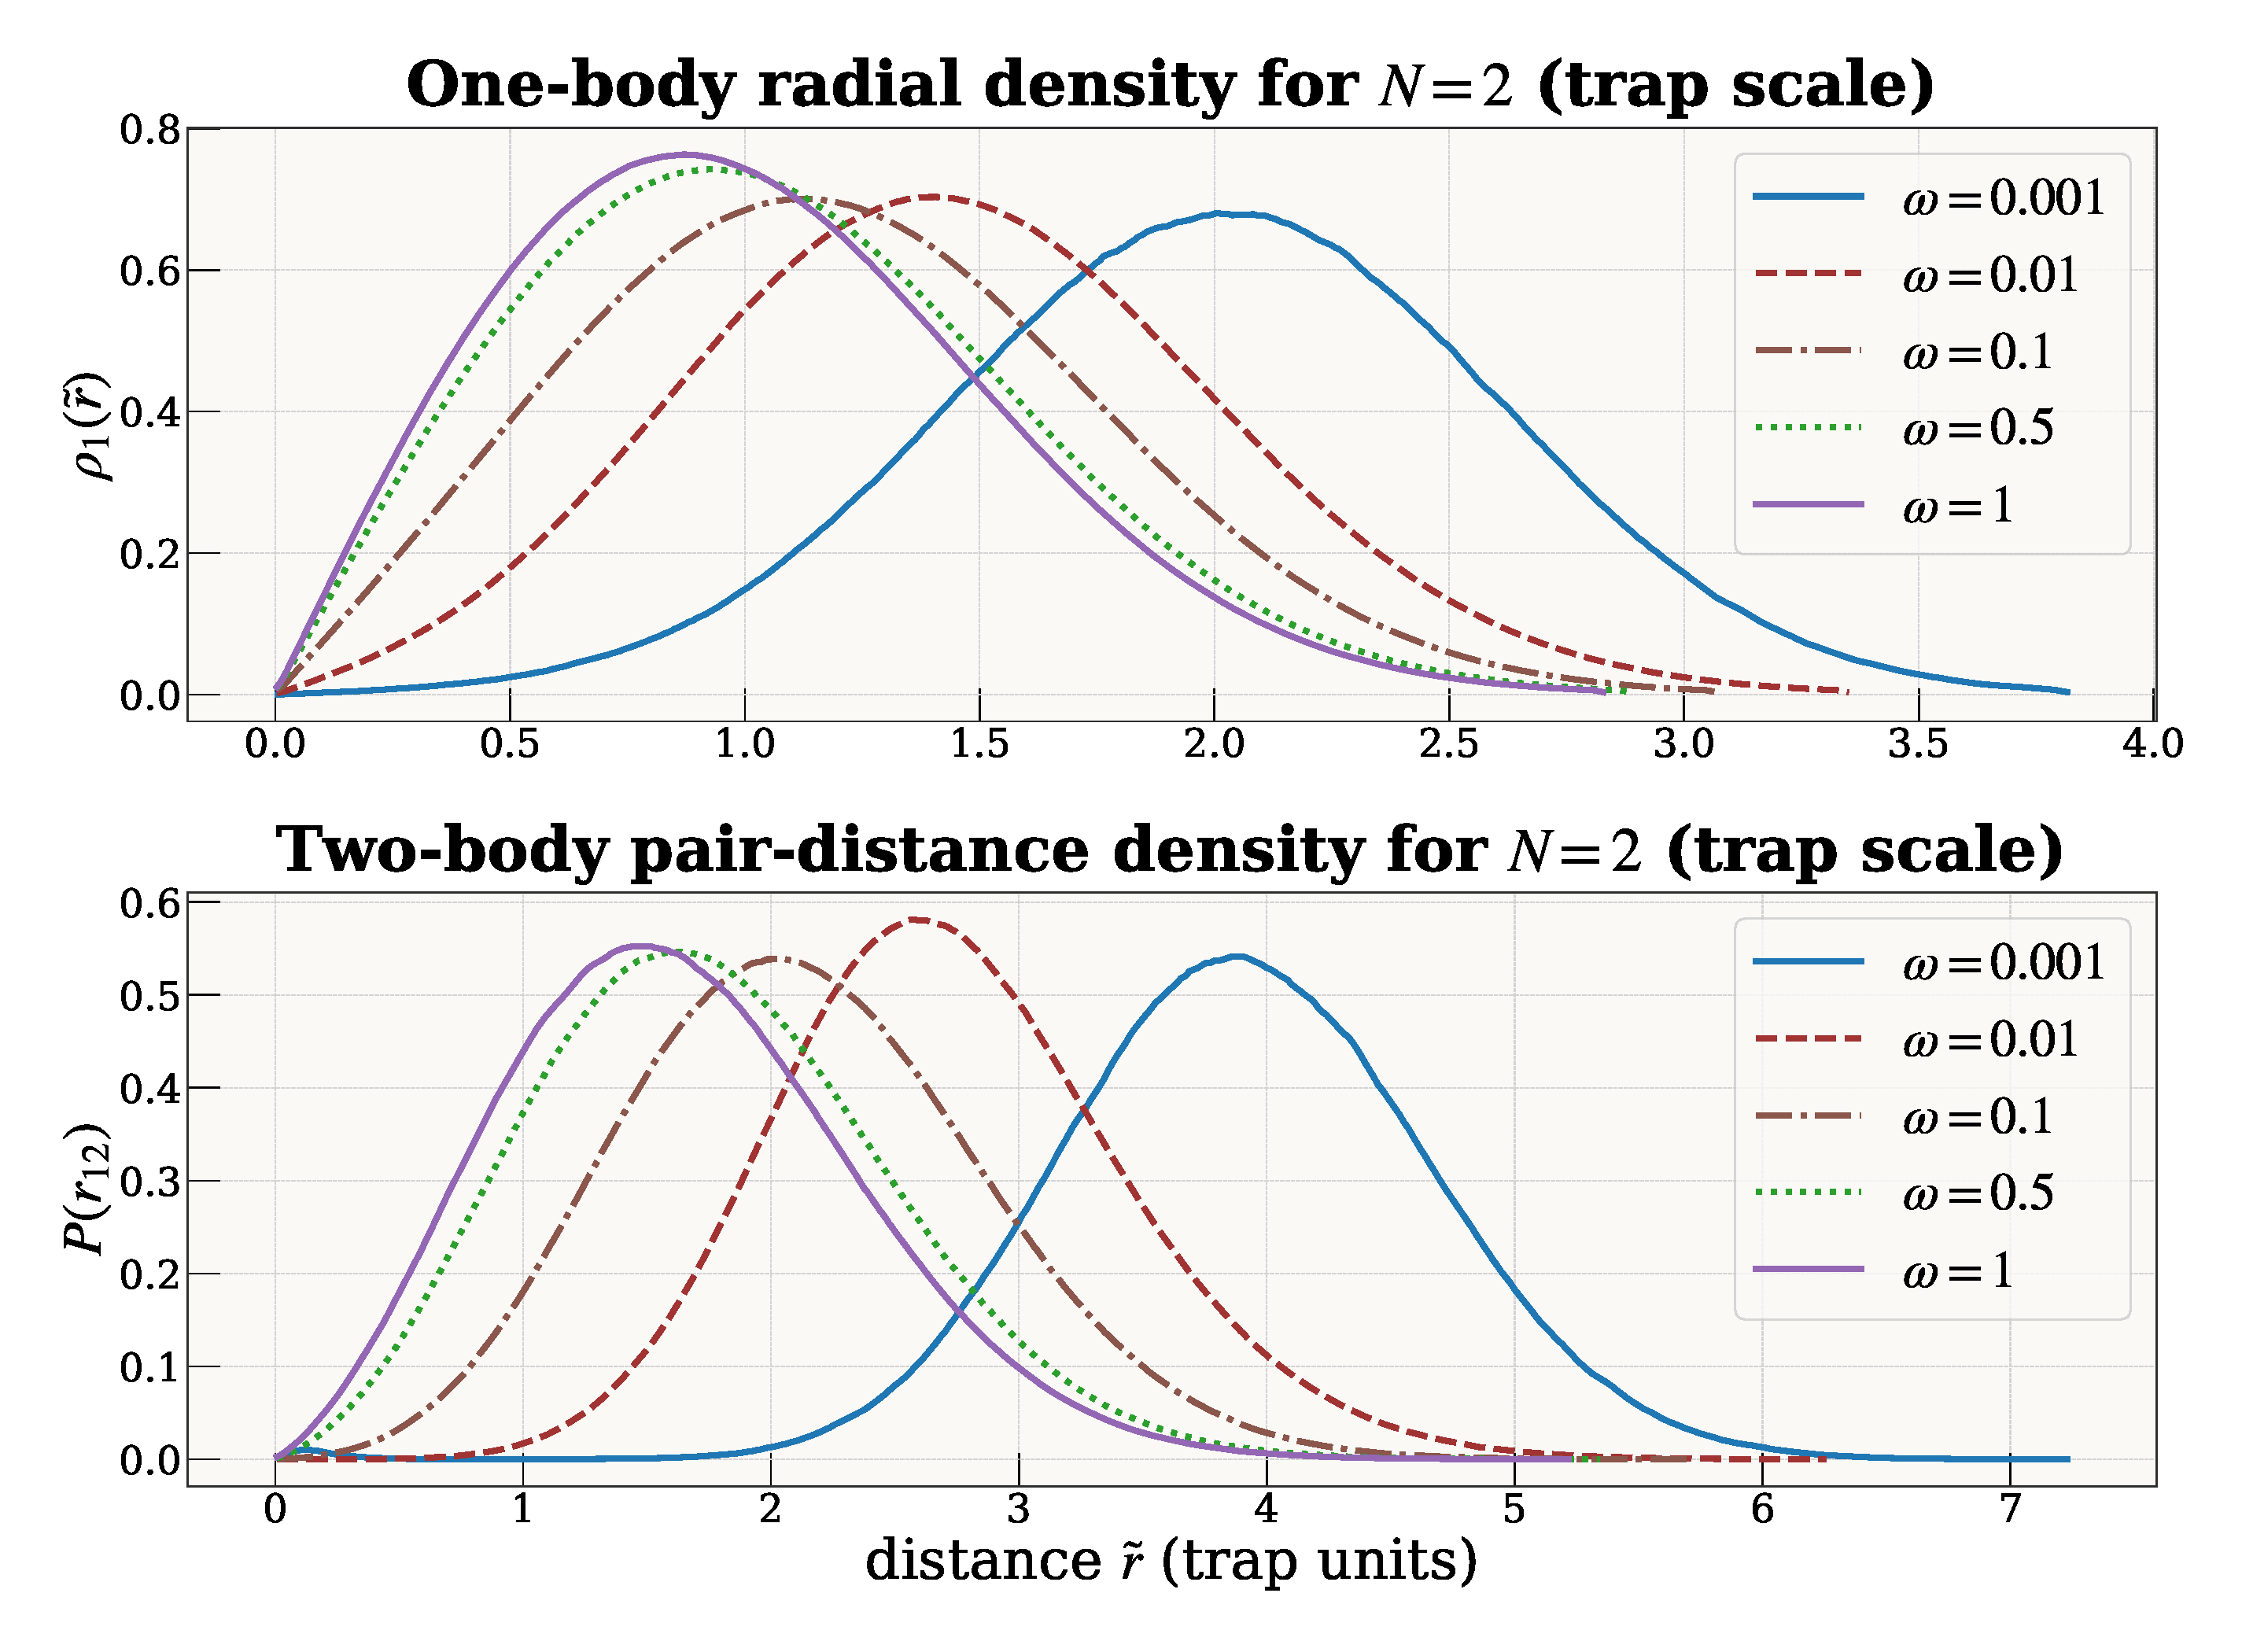
\includegraphics[width=0.9\textwidth]{N2_all_densities}
  \caption[Two-electron radial and pair-distance densities]{One-body radial density
  $\rho_1(\tilde r)$ (top) and pair-distance density $P(r_{12})$ (bottom) for $N{=}2$ across
  $\omega$, in trap units $\tilde r=\sqrt\omega\,r$.}
  \label{fig:2N_radial_densities}
\end{figure}

\begin{figure}[htp]
  \centering
  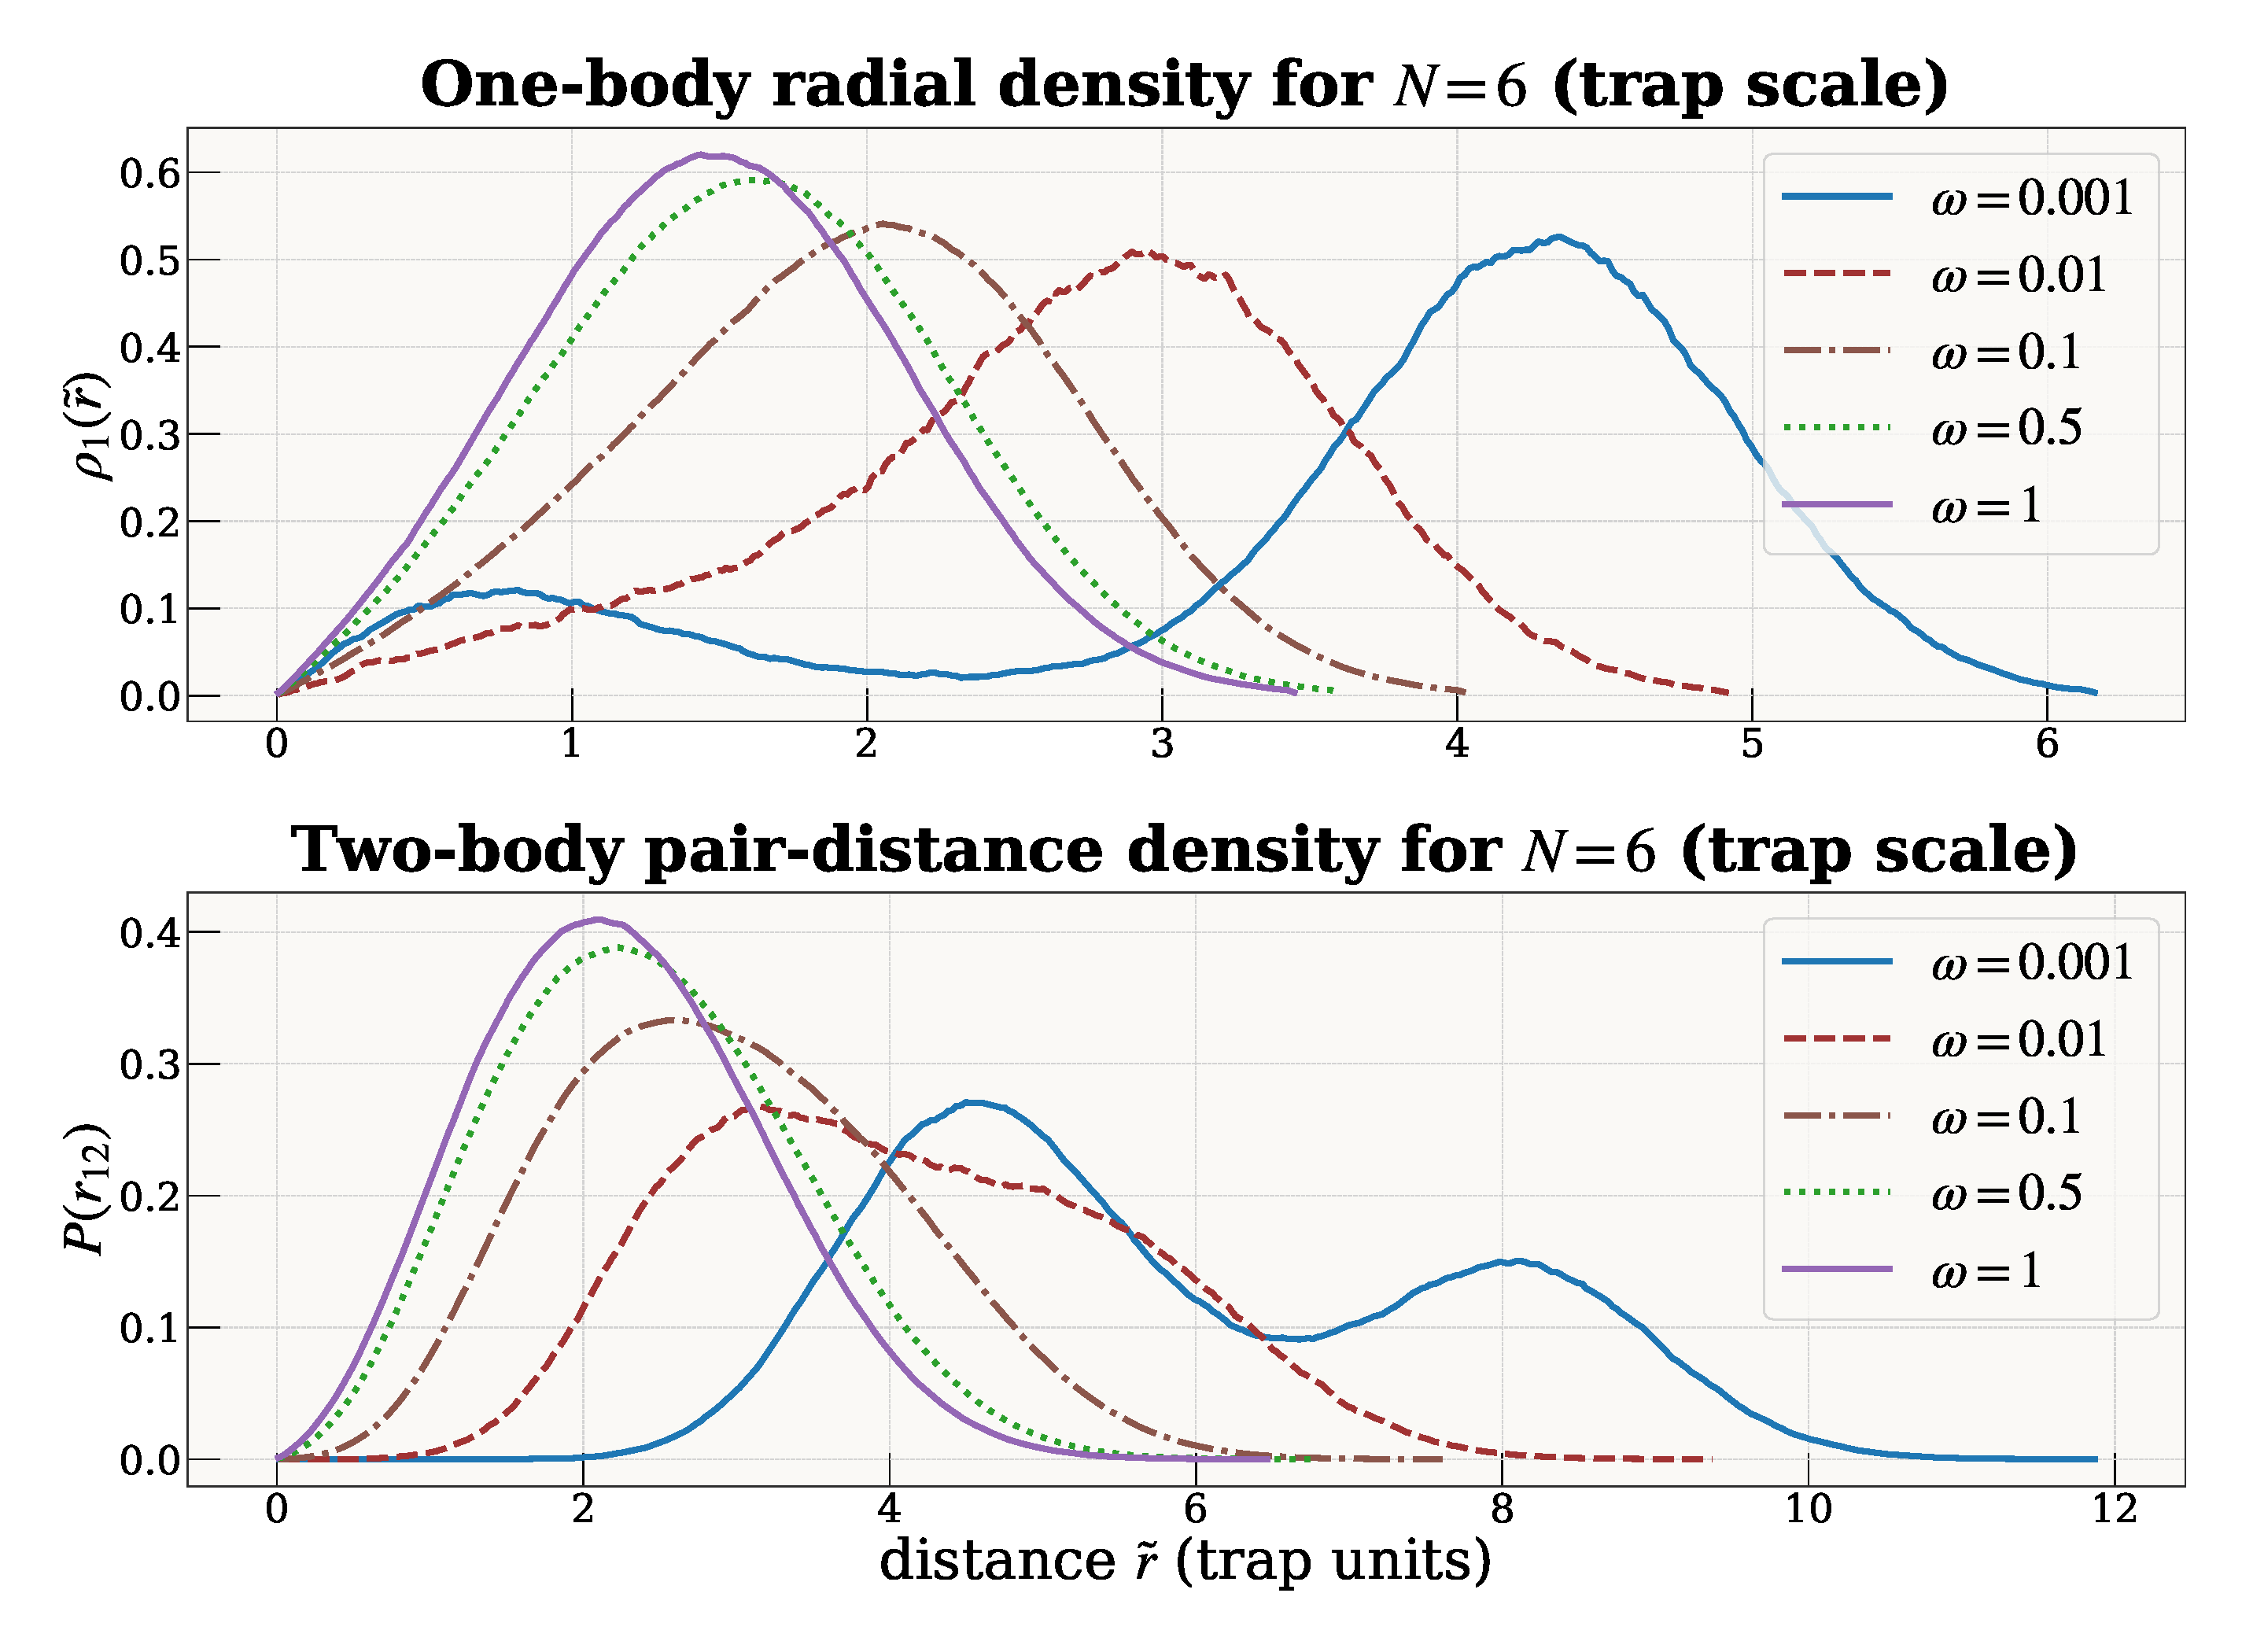
\includegraphics[width=0.9\textwidth]{N6_all_densities}
  \caption[Six-electron radial and pair-distance densities]{As
  Fig.~\ref{fig:2N_radial_densities}, for $N{=}6$. At $\omega=10^{-3}$ the one-body density
  separates into the central electron and the ring, and the pair distribution splits into
  centre--ring and nearest-neighbour distances (first peak) and cross-ring distances
  (second).}
  \label{fig:6N_radial_densities}
\end{figure}

% ──────────────────────────────────────────────────────────────────────
\subsection[Shell topology and angular order]{Shell topology, angular order, and the rotating Wigner molecule}
\label{sec:wigner-angular}

The densities plotted above look like smooth rings, yet the electrons are localised. Both
are true, and the reason is symmetry. Because the Hamiltonian is rotationally invariant, so is its ground state, and any lab-frame
average necessarily smears an angularly ordered configuration into a featureless
ring. The order is real; it simply lives in relative coordinates, and looking for it
in the lab frame is looking in the one place it is guaranteed not to be. Everything
below follows from taking that seriously.

Concretely, a Wigner molecule's internal angular order can only be observed after
registering frames to a co-rotating reference.
For a shell $s$ with $n_s$ particles we compute a rotation-registered
bond-orientational parameter $|\Phi_{n_s}|$ and a corresponding
Lindemann-type ratio quantifying angular stiffness.  Lab-frame densities
remain ring-like (the ``rotating Wigner molecule'' scenario), while the
co-rotating frame reveals crystal-like polygon
order~\cite{Egger_1999,manninen2007metalclustersquantumdots}.

\paragraph{$N{=}6$: single ring with sector mixing.}
At $\omega=0.01$ the system fluctuates between a $(1,5)$ sector (fraction
$\approx 0.69$) and a $(0,6)$ single-ring sector (fraction $\approx 0.31$),
with bond order $|\Phi_5|=0.453\pm0.214$ and $|\Phi_6|=0.466\pm0.206$
respectively. Two conventions apply here and below. The quoted $\pm$ is the frame-to-frame
standard deviation of $|\Phi_m|$, not a standard error on its mean, which with $3\times10^4$
frames is smaller by two orders of magnitude. And these are \emph{sector-conditioned} values,
computed on the frames assigned to that sector in an earlier analysis pass than the
modal-topology values of Appendix~\ref{app:structural-tables:shells}; the two estimators are
set side by side in Table~\ref{tab:bondorder-estimators}. Both must be read against the random-angle
null, the exact mean of $|\Phi_n|$ for independent uniform angles
(Eq.~\eqref{eq:phi-null}), which is $0.402$ for $n{=}5$ and $0.366$ for $n{=}6$: the ratios
here are $1.13$ and $1.27$, so the measured bond order at $\omega=0.01$
exceeds the random-angle value by a modest margin rather than sitting on it.
At $\omega=10^{-3}$ the ring stiffens further:
$(1,5)$ fraction $\approx 0.80$, $(0,6)\approx 0.20$, with
$|\Phi_5|=0.597\pm0.224$ (Lind$\,\approx\!0.225$) and
$|\Phi_6|=0.663\pm0.183$ (Lind$\,\approx\!0.205$)---now far above the random-angle null,
by factors of $1.49$ and $1.81$. This is the confinement at which $n$-fold angular order
becomes \emph{large} rather than merely resolvable
(Appendix~\ref{app:structural-tables:shells}). The distinction matters because with
$10^4$--$10^6$ frames a $2\%$ excess over the null is already resolved at tens of standard
errors; detectability is therefore not what separates the regimes, magnitude is.
Classically $(1,5)$ is the ground-state topology and $(0,6)$ a proximate
competitor; the observed quantum mixture mirrors this
hierarchy~\cite{schweigert1994spectralpropertieschargedparticles,Kong_2002}.
In both weak-trap cases the global $g(r)$ is reproduced to numerical
precision by the appropriate inner--inner / inner--outer / outer--outer (II/IO/OO) mixtures.

\paragraph{$N{=}12$: two shells and commensurability.}
At $\omega=0.01$ two-shell formation is already frequent (fraction $0.761$ at
radial-gap threshold $\tau{=}3.0$), distributed across sectors
$(1,11)=32.6\%$, $(2,10)=25.7\%$, $(3,9)=13.7\%$.
At $\omega=10^{-3}$ shelling becomes ubiquitous
($f_{\rm 2shell}\!\approx\!0.99$--$0.92$ for $\tau=2.0$--$3.0$) and the
\emph{commensurate} $(3,9)$ split emerges as modal ($43.3\%$ of quality-cut
frames), with strong bond order on both rings:
$|\Phi_3|=0.687\pm0.229$ (Lind$_{\rm in}=0.223$),
$|\Phi_9|=0.526\pm0.194$ (Lind$_{\rm out}=0.224$).
Whether the shell picture actually explains the pair structure needs a test that could
fail, and the obvious one cannot. Recombining the inner--inner, inner--outer and
outer--outer histograms with the combinatorial weights of the ideal $(3,9)$ topology
reproduces the global $g(r)$ essentially exactly---but the sector histograms and the total
are accumulated from the same frames, so that recombination is close to exact by
construction. It establishes that the sector bookkeeping is self-consistent, nothing more,
and it is recorded in Appendix~\ref{app:structural-tables:mixfit} for that reason.

The test that can fail is generative and held out (Table~\ref{tab:shell-model-fit-main}).
Shell radii and widths are fitted on half the frames; each shell is modelled as a regular
$n_s$-gon carrying a per-frame global rotation and a fitted angular jitter; and the model is
scored on the other half. It reproduces the pair distribution to cosine similarity
$0.987$--$0.999$ across the whole grid, against $0.936$--$0.996$ for an angle-randomised
null built from the same fitted radial distributions. The difference between them,
$\Delta\cos$, is what \emph{angular} order buys over shell radii alone, and it grows
monotonically as the trap weakens at every particle number---at $N{=}12$ from $0.006$ at $\omega=1$ to $0.026$ at $\omega=10^{-3}$, at $N{=}6$ from
$0.012$ to $0.058$, at $N{=}20$ from $0.003$ to $0.010$. Shell radii alone account for most
of the pair structure at strong confinement; angular structure accounts for a growing
remainder as the molecule forms. How firmly is a separate question, because the smallest
values are a few thousandths, and it was tested directly
(Appendix~\ref{app:structural-tables:mixfit}). Every $\Delta\cos$ carries a block-bootstrap
interval that excludes zero---at $N{=}20$, $\omega=1$ it is $[0.0027,0.0030]$---and the
growth with $1/\omega$ is resolved at every particle number. It survives changes of histogram
binning and of the train/test split essentially unchanged. What does move it is the
angular-jitter model, by up to a third, and the shell threshold where that changes the
partition; the size of $\Delta\cos$ is model-dependent, its sign and its trend are not.

That growth has a different shape from the bond order. $\Delta\cos$ rises by a factor of
$1.1$--$2.1$ per decade at every particle number, monotonically and without a threshold,
whereas the bond order stays flat at its null and then jumps. The two are not in conflict:
$\Delta\cos$ responds to \emph{any} angular correlation that improves the pair-distance
density, while $|\Phi_n|$ responds specifically to $n$-fold order on a registered ring. Weak
angular correlations build gradually from strong confinement onward, and crystalline $n$-fold
order emerges from them only in the final decade---three stages, not a single threshold, with
the middle one measured by a quantity whose sign and trend are robust but whose size depends
on the shell model.

\begin{table}[htbp]
\centering
\caption[Held-out shell-model fit against an angle-randomised null]{The structural test
that can fail. Shell radii and widths are fitted on half the frames; each detected shell is
then modelled as a regular $n_s$-gon carrying a per-frame global rotation and a fitted
angular jitter; and the resulting pair-distance density is scored on the \emph{held-out}
half. $\cos_{\rm poly}$ is the polygon model's agreement with the empirical density and
$\cos_{\rm uni}$ that of an angle-randomised null with the same fitted radial
distributions, so $\Delta\cos$ isolates what polygonal order contributes over shell radii
alone. The interval is a $95\%$ block bootstrap over frames that refits the model and draws
a fresh model sample in every replicate; the tabulated point uses the original single model
sample, whose Monte Carlo noise is part of what the interval measures, so a point can sit
near an edge. Sensitivity to binning, split, shell threshold and jitter model is in
Appendix~\ref{app:structural-tables:mixfit}, with the full table and residuals.}
\label{tab:shell-model-fit-main}
\small
\setlength{\tabcolsep}{6pt}
\begin{tabular}{ccl cccc}
\toprule
$N$ & $\omega$ & occ. & $\cos_{\rm poly}$ & $\cos_{\rm uni}$ & $\Delta\cos$ & $95\%$ interval \\
\midrule
6 & $1.0$ & $1,5$ & $0.9988$ & $0.9866$ & $\mathbf{0.0122}$ & $[0.0122,\,0.0136]$ \\
6 & $0.5$ & $1,5$ & $0.9986$ & $0.9836$ & $\mathbf{0.0150}$ & $[0.0147,\,0.0160]$ \\
6 & $0.1$ & $1,5$ & $0.9974$ & $0.9741$ & $\mathbf{0.0234}$ & $[0.0219,\,0.0236]$ \\
6 & $0.01$ & $1,5$ & $0.9922$ & $0.9536$ & $\mathbf{0.0386}$ & $[0.0371,\,0.0395]$ \\
6 & $0.001$ & $1,5$ & $0.9942$ & $0.9358$ & $\mathbf{0.0585}$ & $[0.0556,\,0.0592]$ \\
\midrule
12 & $1.0$ & $1,11$ & $0.9993$ & $0.9937$ & $\mathbf{0.0056}$ & $[0.0054,\,0.0059]$ \\
12 & $0.5$ & $1,11$ & $0.9990$ & $0.9927$ & $\mathbf{0.0063}$ & $[0.0060,\,0.0066]$ \\
12 & $0.1$ & $1,11$ & $0.9980$ & $0.9896$ & $\mathbf{0.0085}$ & $[0.0083,\,0.0088]$ \\
12 & $0.01$ & $1,11$ & $0.9929$ & $0.9805$ & $\mathbf{0.0124}$ & $[0.0124,\,0.0132]$ \\
12 & $0.001$ & $3,9$ & $0.9868$ & $0.9604$ & $\mathbf{0.0264}$ & $[0.0258,\,0.0271]$ \\
\midrule
20 & $1.0$ & $1,19$ & $0.9992$ & $0.9964$ & $\mathbf{0.0028}$ & $[0.0027,\,0.0030]$ \\
20 & $0.5$ & $1,19$ & $0.9990$ & $0.9958$ & $\mathbf{0.0032}$ & $[0.0030,\,0.0033]$ \\
20 & $0.1$ & $1,19$ & $0.9982$ & $0.9942$ & $\mathbf{0.0040}$ & $[0.0038,\,0.0040]$ \\
20 & $0.01$ & $1,19$ & $0.9947$ & $0.9900$ & $\mathbf{0.0047}$ & $[0.0046,\,0.0049]$ \\
20 & $0.001$ & $1,7,12$ & $0.9915$ & $0.9820$ & $\mathbf{0.0095}$ & $[0.0091,\,0.0095]$ \\
\bottomrule
\end{tabular}
\end{table}



\begin{figure}[htp]
  \centering
  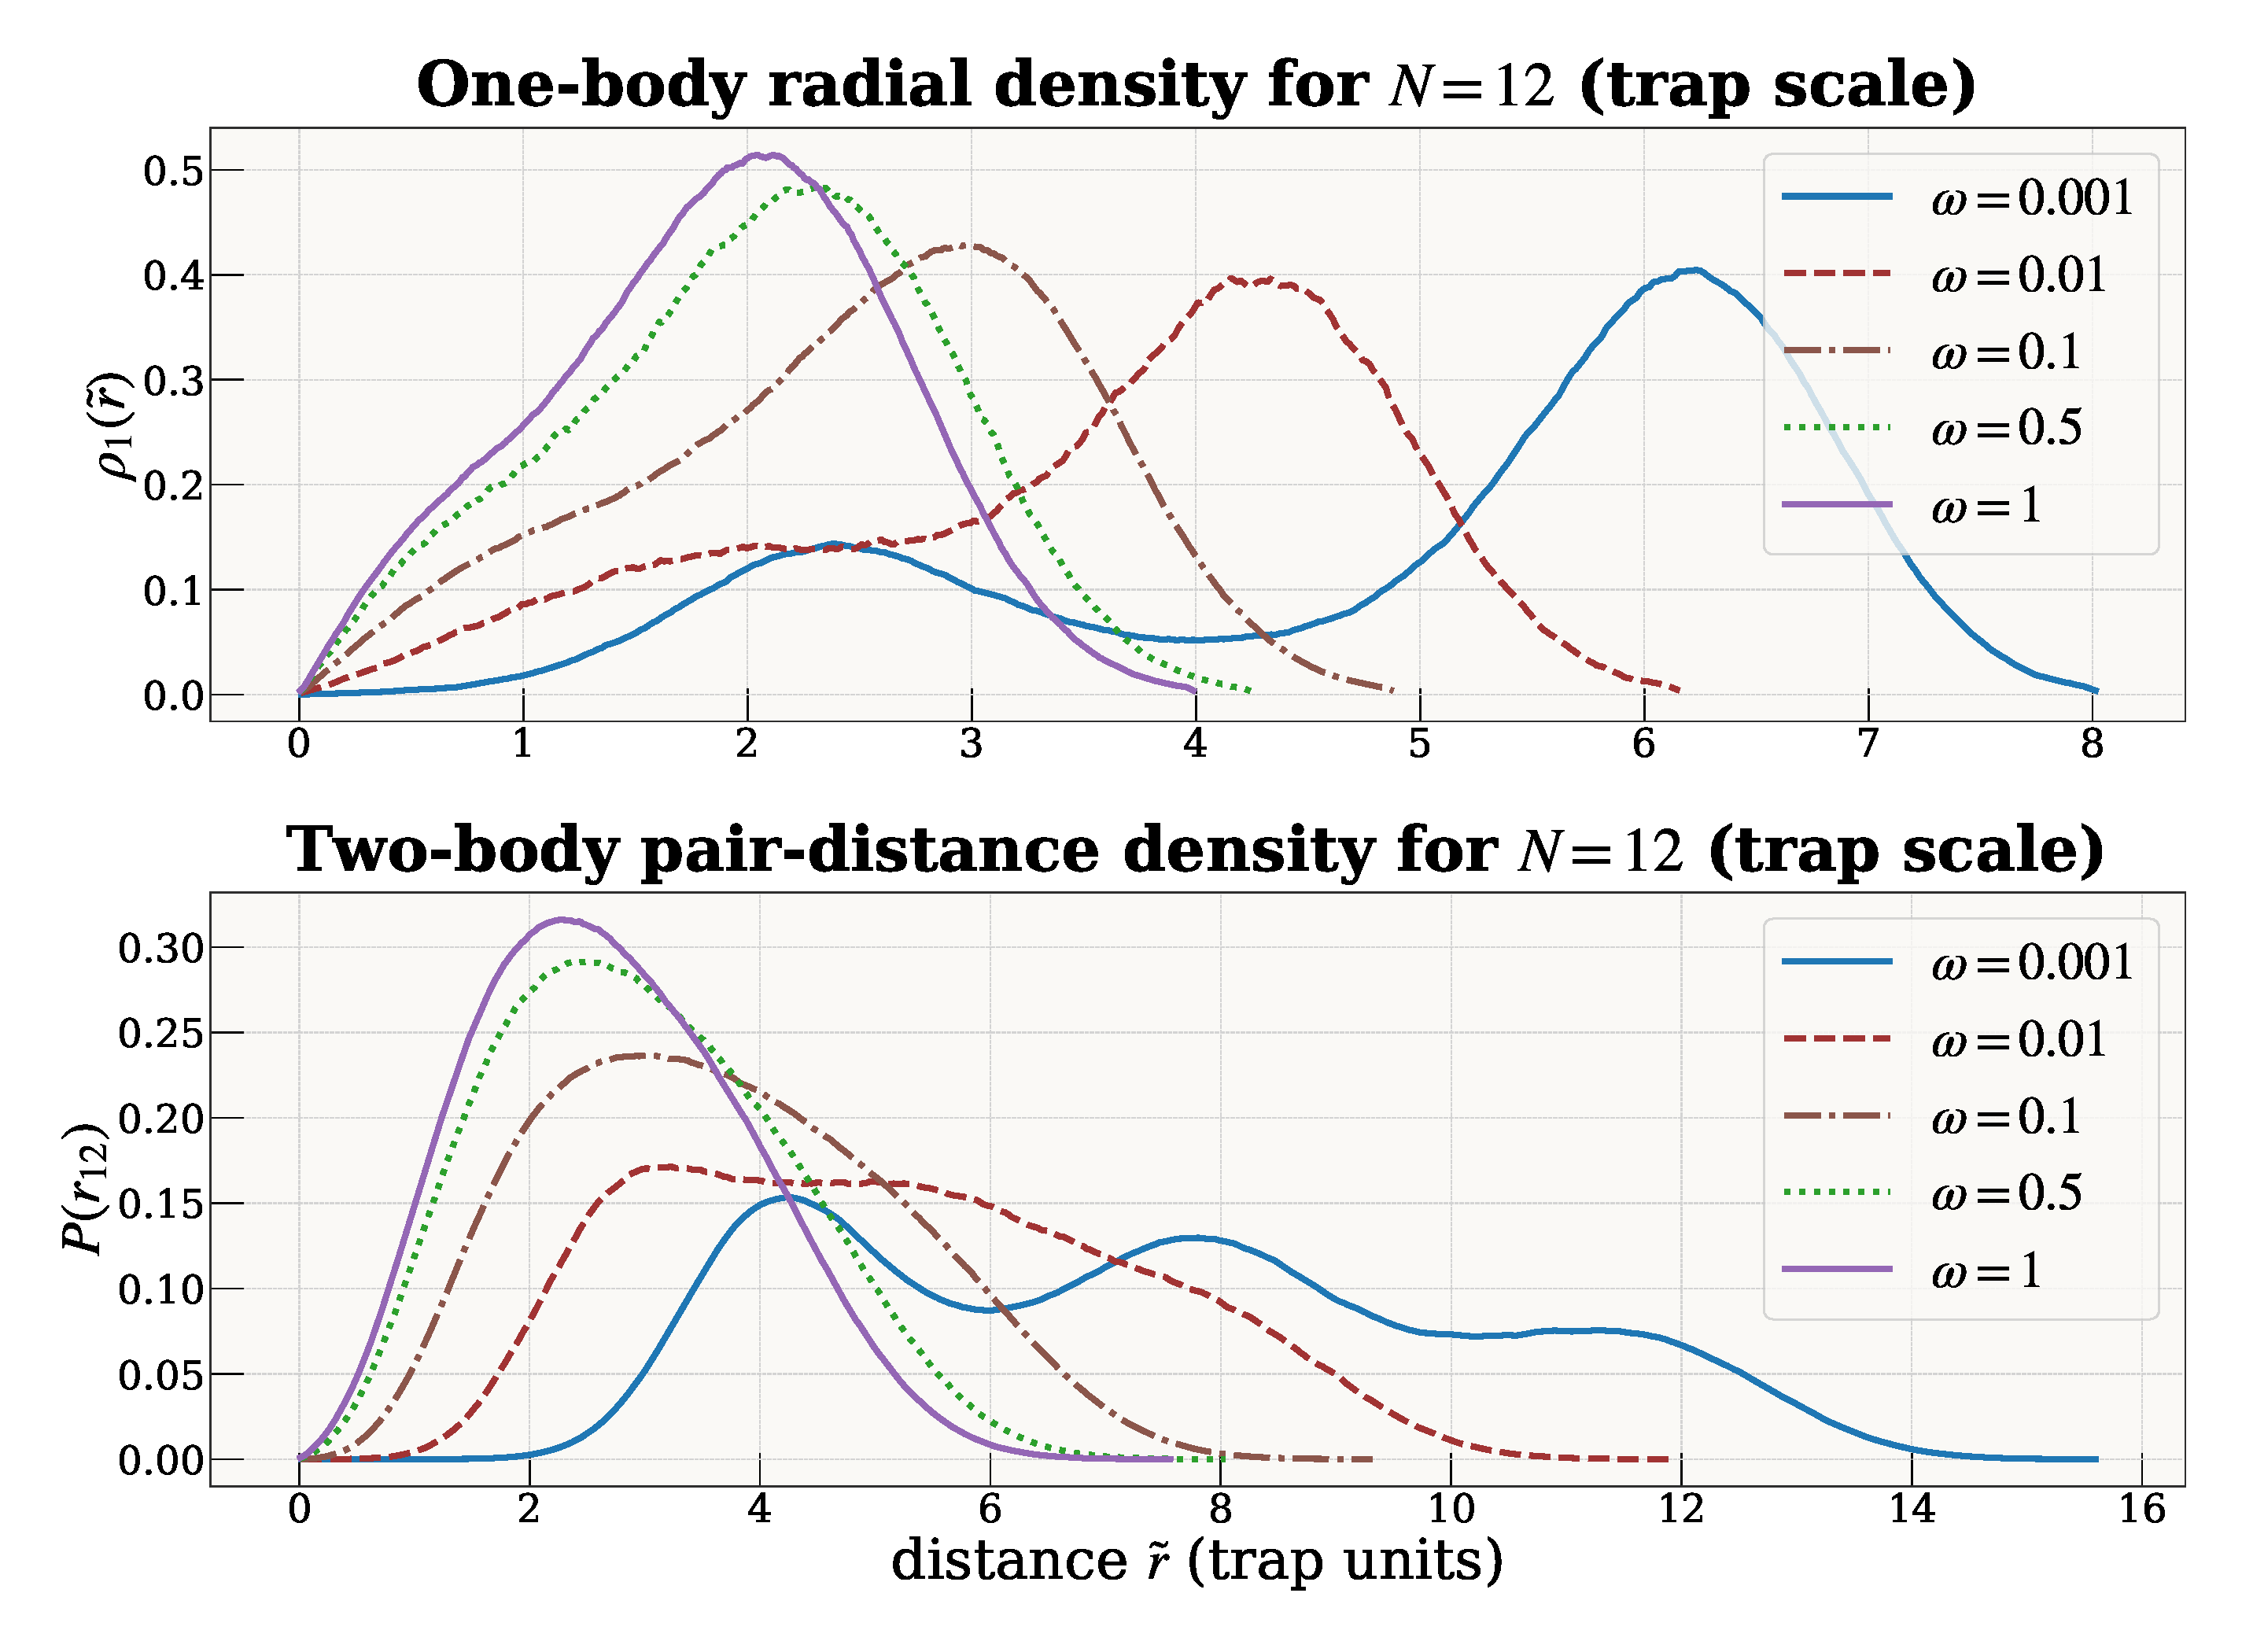
\includegraphics[width=0.9\textwidth]{N12_all_densities}
  \caption[Twelve-electron radial and pair-distance densities]{As
  Fig.~\ref{fig:2N_radial_densities}, for $N{=}12$.}
  \label{fig:12N_radial_densities}
\end{figure}

\paragraph{$N{=}20$: three-shell molecule and a rapid radial reorganisation.}
At $\omega=10^{-3}$ the dominant shell topology is $(1,7,12)$---a clear
three-shell Wigner molecule with widely separated rings at radii
$r_0\approx38$, $r_1\approx132$, $r_2\approx247$
(gaps $\approx94$ and $\approx115$).
The lab-frame pinning metric remains small ($C_{\mathrm{global}}\approx0.06$), as expected
for a freely rotating molecule. That number also answers a question the ansatz raises. Its
displacement head is not rotation-equivariant by construction (\S\ref{sec:bf-init}), so a
trained state could in principle carry an orientation fixed to the lab frame and read as
angular order; such a state would show a large $C_{\mathrm{global}}$, and this one does not.
The order the per-shell moduli measure is internal to the molecule. The cross-shell quantity $\tilde C_{\mathrm{global}}$ is
omitted: it depends on a registration convention whose original analysis code was not
retained (\S\ref{subsec:orient}). The per-shell moduli and angular-spacing diagnostics below
are rotation-invariant and carry no such dependence.
Lindemann disorder on the two occupied outer shells is low:
$L_{7,\mathrm{reg}}\approx0.35$ and
$L_{12,\mathrm{reg}}\approx0.27$.

Already at $\omega=10^{-2}$ the radial gap detector returns a $(1,19)$ partition rather than
a three-shell one: the shell radii contract by an order of magnitude ($r_0\approx10$,
$r_1\approx45$), the outer-shell angular disorder rises to $\approx0.57$. The wording
matters here. At $\omega=10^{-3}$ the $(1,7,12)$ label describes a
Wigner \emph{topology}, because it is accompanied by separated shells, registered angular
order and low Lindemann disorder. At $\omega=10^{-2}$ and above, with angular order at its
random-angle null and disorder high, $(1,19)$ is what the \emph{radial classifier returns}
on a state that is not angularly ordered at all---a decomposition of the radial density, not
a crystalline shell structure. We use the occupancy notation in both cases because the
detector does, but only the weakest-trap case earns the word topology.
At $\omega=1$ the classifier returns the same $(1,19)$ partition, with compact radii
($r_0\approx0.55$, $r_1\approx2.3$) and high angular disorder
($L_{\rm out}\approx0.69$).
What the data show, then, is a rapid radial reorganisation somewhere between
$\omega=10^{-3}$ and $10^{-2}$, not a collapse of one crystalline topology into another: the
state at $10^{-2}$ has no demonstrated angular order to lose. How rapid, and where in that
decade it happens, the grid cannot say. It samples one point per decade, and the radial
classifier reports a partition at each point rather than tracking a structure between them.

\subsection{The crossover across diagnostics}
\label{sec:wigner-synthesis}

Six diagnostics, applied at four particle numbers and five confinements, agree. As $\omega$
falls from $1$ to $10^{-3}$ the densities expand and develop rings, and the shell topology
resolves into the discrete finite-$N$ patterns that classical Coulomb clusters
predict---$(1,5)$ at $N{=}6$, $(3,9)$ at $N{=}12$, $(1,7,12)$ at
$N{=}20$~\cite{schweigert1994spectralpropertieschargedparticles,Kong_2002}. The shells
separate and stiffen. The Lindemann disorder falls monotonically throughout, while
rotation-registered bond order stays within $1\%$ of its random-angle null down to
$\omega=0.1$ and reaches $1.16$--$1.63$ times it only at $\omega=10^{-3}$
(Appendix~\ref{app:structural-tables:shells}). Radial stiffening precedes $n$-fold angular ordering instead of accompanying it. Lab-frame order stays near zero throughout, as
expected for a freely rotating molecule.
The energy partitioning approaches the classical virial form, with $\Gamma$ reaching
${\sim}40$ for $N{=}12$ at the weakest trap. None of these was built into the ansatz. The commensurate $(3,9)$ sector at $N{=}12$ carries real weight in
$(1,11)$ and $(2,10)$ besides, which is the quantum rotational mixing the rotating-Wigner-molecule
picture
predicts~\cite{manninen2007metalclustersquantumdots,Filinov_2001}. At $N{=}20$ the
three-shell structure at $\omega=10^{-3}$ gives way, by $\omega=10^{-2}$, to a radial
partition of a state without angular order; the grid is too coarse to place that
reorganisation more finely than within the decade. The $(1,7,12)$ configuration itself is not new. It is the known classical shelling, reported in quantum calculations of comparable dots, and no novelty is claimed for it. What we have not found
reported elsewhere for $N\ge12$ parabolic dots is the combination of \emph{sector-conditioned}
bond-order and Lindemann statistics, read against their random-angle null, with a held-out
polygon reconstruction of $g(r)$ scored against an angle-randomised baseline.

The diagnostics do not carry equal weight, and they do not all support the same claims.
Table~\ref{tab:wigner-evidence} sets out which one carries which statement and how firmly.
The strongest evidence is at the deepest Wigner points; the qualitative staging is better
established than where, within the coarse $\omega$ grid, each stage sets in.

\begin{table}[htbp]
\centering
\caption[Which diagnostic supports which claim]{Which diagnostic supports which claim about
the crossover. ``Firm'' means a large effect in a state-level or shell-resolved quantity;
``weak'' marks evidence that is suggestive but small or carried by a quantity known to
mix structures.}
\label{tab:wigner-evidence}
\small
\renewcommand{\arraystretch}{1.2}
\begin{tabular}{@{}>{\raggedright\arraybackslash}p{0.29\textwidth}
                >{\raggedright\arraybackslash}p{0.42\textwidth}
                >{\raggedright\arraybackslash}p{0.21\textwidth}@{}}
\toprule
Claim & Carried by & Strength \\
\midrule
The cloud expands faster than the non-interacting $\omega^{-1/2}$ &
rms radius from $\langle V_{\rm trap}\rangle$; $r_{\rm mode}$ exponent &
firm, all $N$ \\
Interactions take over &
$\Gamma=\langle V_{\rm int}\rangle/\langle T\rangle$ rises tenfold &
firm, $N\le12$ \\
Classical force balance emerges &
$2\langle V_{\rm trap}\rangle/\langle V_{\rm int}\rangle\to1.23,\,1.07,\,1.05$ &
firm at $N{=}12$ \\
Shells stiffen radially &
shell-resolved widths ($N{=}6$ ring: $0.32\to0.15$) and pair Lindemann ratios; global
$\gamma$ only at $N{=}2$ &
firm; global $\gamma$ weak at $N{=}6$ \\
The ring approaches its classical radius &
outer radius over $1.334\,\omega^{-2/3}$: $1.247\to1.017$ &
firm, $N{=}6$ \\
Discrete Wigner topologies form &
radial classifier with registered order: $(1,5)$, $(3,9)$, $(1,7,12)$ &
firm at $10^{-3}$; above it, radial partitions only \\
Weak angular correlation builds gradually &
held-out polygon model against angle-randomised null, $\Delta\cos$ (block bootstrap) &
firm in sign and trend; size depends on the jitter model \\
$n$-fold angular order appears late &
$|\Phi_n|$ against its exact null, which is also the pipeline's null &
firm at $10^{-3}$; absent above $0.1$ (resolved departures ${\lesssim}1\%$) \\
Where each stage sets in &
one grid point per decade &
not established \\
\bottomrule
\end{tabular}
\end{table}

Two qualifications bound all of it. The states are the lowest we find within a fixed
spin-projection sector, and we have not scanned total spin, so these are not proven
global-spin ground states. And the combinatorial reconstruction of $g(r)$ establishes
decomposability rather than sampling correctness; the held-out polygon fit of
Appendix~\ref{app:structural-tables:mixfit} is the version that could have failed, and
sampling correctness itself rests on the independent restart and chain diagnostics.

The two angular diagnostics stage the crossover slightly differently, and the difference is
informative. Radial localisation (expansion, shell separation, falling shell-resolved width, classical force balance) develops progressively from $\omega=1$ down.
Bond-orientational order is flat at its null through $\omega=0.1$, departs at $\omega=0.01$
clearly only at $N{=}6$, and becomes large at $10^{-3}$ everywhere. The held-out
polygon model, sensitive to any angular correlation rather than to $n$-fold order
specifically, instead grows monotonically throughout, roughly doubling per decade. Read at
face value, weak angular correlations build gradually across the whole range while
\emph{crystalline} $n$-fold order appears only in the last decade: a three-stage picture
rather than a two-stage one. The two-stage separation of radial and $n$-fold angular order
is the firmer statement; the gradual middle stage is resolved in sign and trend, but its size
depends on the shell model used to measure it.

These structural facts then enter the method. The shell radius approaching its classical
$\omega^{-2/3}$ scaling---within $1.7\%$ of the classical prefactor at $\omega=10^{-3}$,
Appendix~\ref{app:structural-tables:radius}---and the angular order sharpening in the last
decade are exactly the quantities a sampler must respect to reach the Wigner regime without a
Markov chain. An origin-centred proposal aims where the wavefunction no longer has any mass;
a proposal built from the measured shell radius and angular order tracks it, and carries
Markov-chain-free training far into the correlated regime
(\S\ref{sec:kernel-q3-frontier}). What the trained model reveals about the physics is what
later lets us train it more cheaply.

That is the state seen from outside. What the network had to hold internally in order to
produce it is a question about the solver, and Chapter~\ref{ch:kernel} takes it up.

% =====================================================================
%  Results chapter: architecture, optimiser, and paradigm through the
%  tangent kernel. UNIFIED draft.
%
%  Supersedes the split between the earlier kernel draft (message
%  passing in the JASTROW) and results_backflow.tex (message passing in
%  the BACKFLOW): both are the same relational-channel idea seen through
%  the tangent kernel, and are merged here. All numbers are on the
%  thesis ansatz at DMC-quality energies; seed counts are stated.
% =====================================================================
\graphicspath{{../results/figures/results/}{../results/figures/results/kernel/}{../results/figures/}}
\chapter{Architecture, optimisation and sampling}
\label{ch:kernel}

The previous chapter showed that the ansatz works: it reaches reference quality wherever it was
compared with a reference, and the states it produces carry the staged Wigner-molecule structure the
diagnostics were built to detect. Why the solver can represent those states, and what
governs whether they can be trained at all, are separate and harder questions.

Three observations from that chapter remain unexplained. Two networks of the same size,
trained the same way and landing on the same energy, need not be the same object. A
natural-gradient step that is decisive in one training regime does nothing in another. And
an importance-sampled objective reproduces a Markov chain's answer in one corner of the
phase diagram and departs from it in the next.

All three can be examined through the per-sample, column-centred log-derivative matrix
\begin{equation}
  O_{ki} \;=\; \frac{\partial \log|\Psi_{\btheta}(\bx_k)|}{\partial \theta_i},
  \qquad k=1,\dots,B,\;\; i=1,\dots,P,
  \label{eq:kernel-O}
\end{equation}
and on its two Gram matrices, the quantum geometric tensor $S = O^{\!\top}O / B$ and the
neural tangent kernel $K = OO^{\!\top}$~\cite{JacotEtAl2018-NTK,StokesEtAl2020-QuantumNaturalGradient}.
That gives the chapter its structure:

\begin{quote}
\emph{Architecture} determines the shape of the tangent space.\\
The \emph{optimiser} acts on it through its metric.\\
The \emph{sampling measure} determines how well that metric can be estimated.
\end{quote}

\noindent The chapter takes them in that order. The instrument throughout is the \emph{effective dimension} of the tangent space---the
participation ratio of the QGT spectrum $\{\lambda_a\}$,
\begin{equation}
  d_{\mathrm{eff}}(S) \;=\; \frac{\left(\sum_a \lambda_a\right)^2}{\sum_a \lambda_a^2},
  \label{eq:deff}
\end{equation}
which counts how many directions actually carry Fisher weight, whatever the parameter
count says. Beside it sit the local-energy variance $\Var(E_L)$, zero only for an exact
eigenstate; the effective sample size; and the condition number $\kappa(S)$, which is
reported in \S\ref{sec:kernel-cond} and turns out to be large everywhere and therefore
diagnostic of nothing by itself.

Architectures are compared on a common probe set---the same configurations for every model,
never each model's own $|\Psi|^2$---and below $\omega=0.1$ every relative error is measured
against our own converged variational energies, so it reports internal consistency rather
than accuracy. The tooling is anchored on the analytic two-electron ground state, where the
ansatz returns $E=3.000127$~Ha ($+0.004\%$) at squared overlap $1.000000$.

% =====================================================================
\section{Message passing and the variational geometry}
\label{sec:kernel-q1}

How do the implemented message-passing and separable model families differ after training?
We ask this separately of the correlator and the backflow. The Slater reference, analytic
cusp and training protocol are shared, but the correlators use different learned pair
features, and the backflows differ in capacity, coordinate preprocessing and centre-of-mass
projection (\S\ref{sec:bf-init}). The comparisons therefore identify differences between the
archived implementations; they do not isolate message routing alone.

\subsection{The correlator: tangent-space compression}
\label{sec:kernel-q1a}

At $N=6$, $\omega=1$ the two correlators are indistinguishable in energy. Trained to DMC
quality across a $20$k--$164$k parameter ladder, every model lands within $\pm0.1\%$ of the
reference, and the best raw energy belongs to a $164$k separable network---twice the
message-passing parameter count. Both have reached the same observed energy floor at this
resolution. That agreement hides two differences developed below: the message-passing
correlator has lower local-energy variance across the confinement range and, under the
chosen parametrisations, concentrates its tangent weight differently.

Their tangent geometry is not indistinguishable. On a common probe set the message-passing
correlator reaches a reference-quality state in $d_{\mathrm{eff}}\approx1.2$--$1.7$ over three seeds,
where every separable network needs $2.9$--$3.6$; the two sets do not overlap, and their
closest approach is still a factor of $1.7$. Capacity does not close the gap. Scaling the
separable network eightfold, from $20$k to $164$k parameters, moves its effective dimension
only from $3.6$ to $2.9$, and the $89$k network that matches the message-passing one in size
sits at $3.6$. The gap moves by at most $0.26$ whether scored on either family's samples or
on pooled points. With three and four runs respectively, we report the values rather than a
sigma-separation.

\begin{figure}[htbp]\centering
  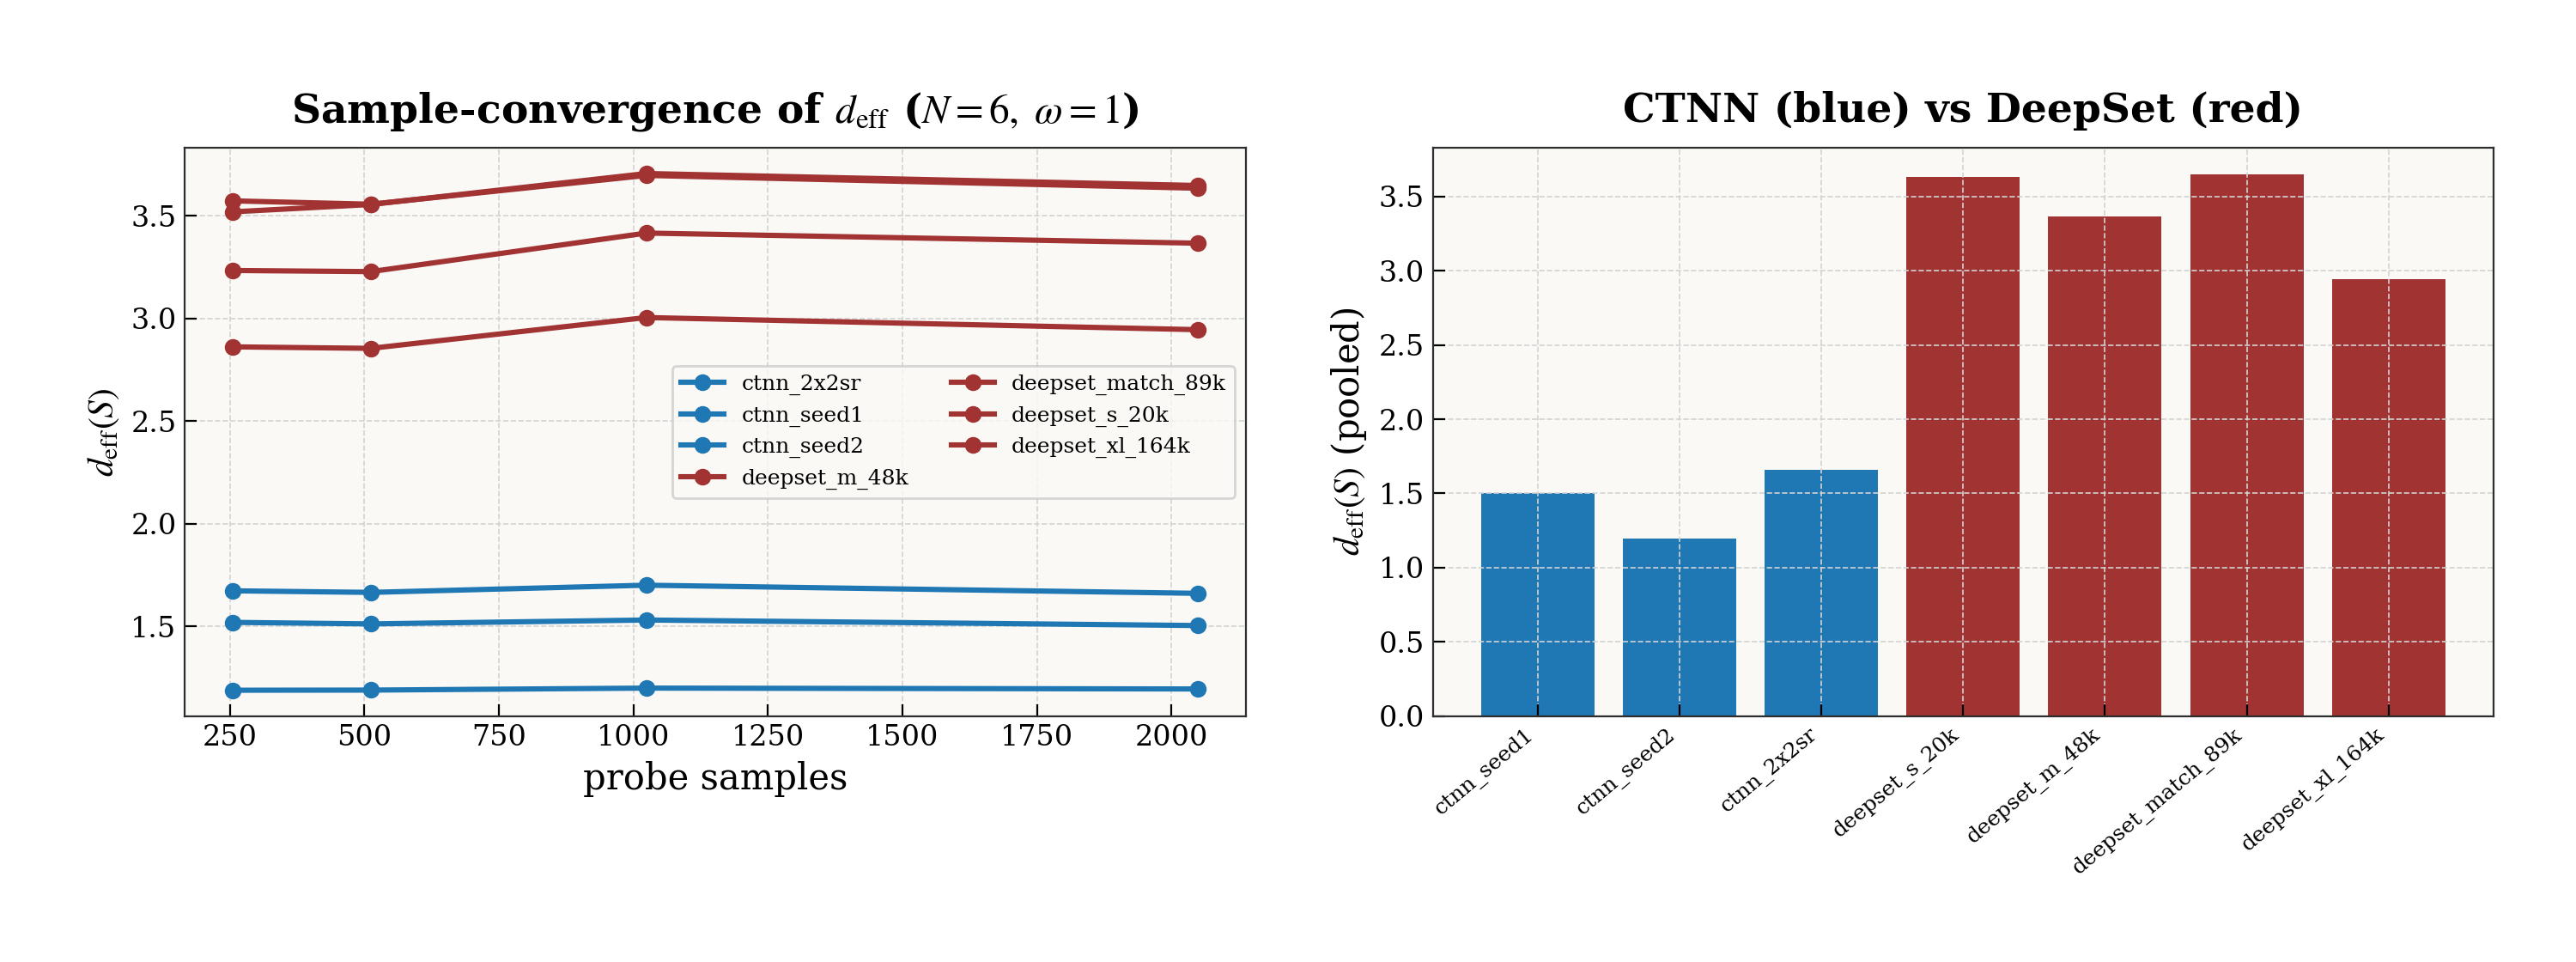
\includegraphics[width=0.95\textwidth]{fair_dimension.png}
  \caption[Message passing concentrates the correlator's Fisher weight]{Effective dimension
  of the correlator's tangent space ($N{=}6$, $\omega{=}1$) on a common pooled probe.
  \emph{Left:} convergence in the number of probe samples. \emph{Right:} per model. The CTNN
  (blue) sits at $d_{\mathrm{eff}}\!\approx\!1.2$--$1.7$ and every DeepSet (red) at
  $\approx\!2.9$--$3.6$; scaling the DeepSet from $20$k to $164$k parameters does not close
  the gap. $d_{\mathrm{eff}}$ depends on the parametrisation (\S\ref{sec:kernel-q1a}).}
  \label{fig:q1a-fairdim}
\end{figure}

The dimension gap is a strong-confinement effect: toward the Wigner crystal both families reach
${\sim}3.7$, although they occupy different tangent subspaces. A single-seed inversion at
the crystal reported in an earlier draft did not survive seeding. Because no backflow is
present here, division of correlation between the correlator and backflow is not at issue.

One more limit applies to every tangent-space quantity in this chapter. The QGT spectrum
depends on the parametrisation: rescaling a layer or changing a normalisation can reweight
tangent directions without changing the state. The result is therefore specific and useful:
under the parametrisations and normalisation conventions used here, the message-passing
correlator concentrates its empirical Fisher weight in fewer directions. It does not show
that the architecture represents the state with intrinsically fewer degrees of freedom.
Only the energy and local-energy variance are state-level comparisons, and only the variance
separates these families.

\paragraph{Local-energy variance.} $d_{\mathrm{eff}}$
stops separating the families at the crystal, and rank will turn out to be gauge-like
(\S\ref{sec:synthesis}). The local-energy variance does neither: it is defined on the
state, vanishes only for an exact eigenstate, and is directly comparable between any two
ansätze evaluated on their own $|\Psi|^2$. Measured at matched training protocol,
$\Var(E_L)$ is lower for the message-passing correlator at every confinement
(Table~\ref{tab:varEL}), by factors between $1.2$ and $3.4$, while the two are
indistinguishable in energy.

At the crystal the three-seed means differ by a factor of $1.8$, rather than the $7.4$
obtained by pairing single best runs. Capacity does not remove the effect: at $\omega=1$ the
capacity-matched $89.4$k separable network widens the ratio to $3.4$. Intermediate
confinements ($\omega=0.28,\,0.05,\,0.03$) preserve the ordering at ratios $1.2$--$1.8$.
The difference is not resolved at the smallest depth-analysis tier ($12$k against $9$k), so
the claim is about trained models at production width, not either architecture at every size.

\begin{table}[htbp]\centering
\caption[Local-energy variance by architecture]{Local-energy variance at $N{=}6$, matched training protocol, both architectures at
reference-quality energy ($|{\rm err}|\le0.13\%$). Lower is better; $\Var(E_L)\to0$ only for
an exact eigenstate. The basis column gives the evidential status of each row: the $\omega=0.01$ row is a
three-seed mean, the rest are single runs of the production cascade. The unseeded rows
establish the ordering, which never reverses, and not the precise factor
(\S\ref{sec:kernel-q1a}). The last row repeats $\omega=1$ against the capacity-matched
$89.4$k separable network.}
\label{tab:varEL}
\begin{tabular}{lcccc}
\hline
$\omega$ & CTNN & DeepSet & ratio & basis \\
\hline
$1.0$  & $1.09\times10^{-2}$ & $2.51\times10^{-2}$ & $2.3$ & single run, $79.8$k vs $47.7$k \\
$0.5$  & $4.62\times10^{-3}$ & $1.01\times10^{-2}$ & $2.2$ & single run, $79.8$k vs $47.7$k \\
$0.1$  & $5.63\times10^{-4}$ & $1.14\times10^{-3}$ & $2.0$ & single run, $79.8$k vs $47.7$k \\
$0.01$ & $1.85\times10^{-5}$ & $3.35\times10^{-5}$ & $1.8$ & 3-seed mean, $79.8$k vs $47.7$k \\
\hline
$1.0$  & $2.75\times10^{-2}$ & $9.38\times10^{-2}$ & $3.4$ & matched, $79.8$k vs $89.4$k \\
\hline
\end{tabular}
\end{table}

\paragraph{Relating the leading tangent directions to selected operators.} At the exact
$N=2$ anchor the selected dictionary describes the leading mode with
$R^2=1.00$, using a breathing mode
($\partial_\omega$), a correlation-hole mode, and the first relative excitation. This is not
special to two bodies. Projecting the leading tangent mode of trained correlators onto a
dictionary of selected operators (breathing/monopole, quadrupole, correlation-hole,
pair-linear), seed-averaged over well-trained checkpoints (energy within $1.5\%$ of
reference), the CTNN reaches $R^2\!\gtrsim\!0.93$ at $N=6$ and $R^2\!\approx\!1.00$ at $N=12$
across the whole confinement range $\omega\in[0.01,1]$, and both architectures reproduce the
$N=2$ naming at strong confinement (Fig.~\ref{fig:mode-naming}). For the message-passing
correlator, the direction carrying most of the tangent weight is well described by this small
dictionary.

\begin{figure}[htbp]\centering
  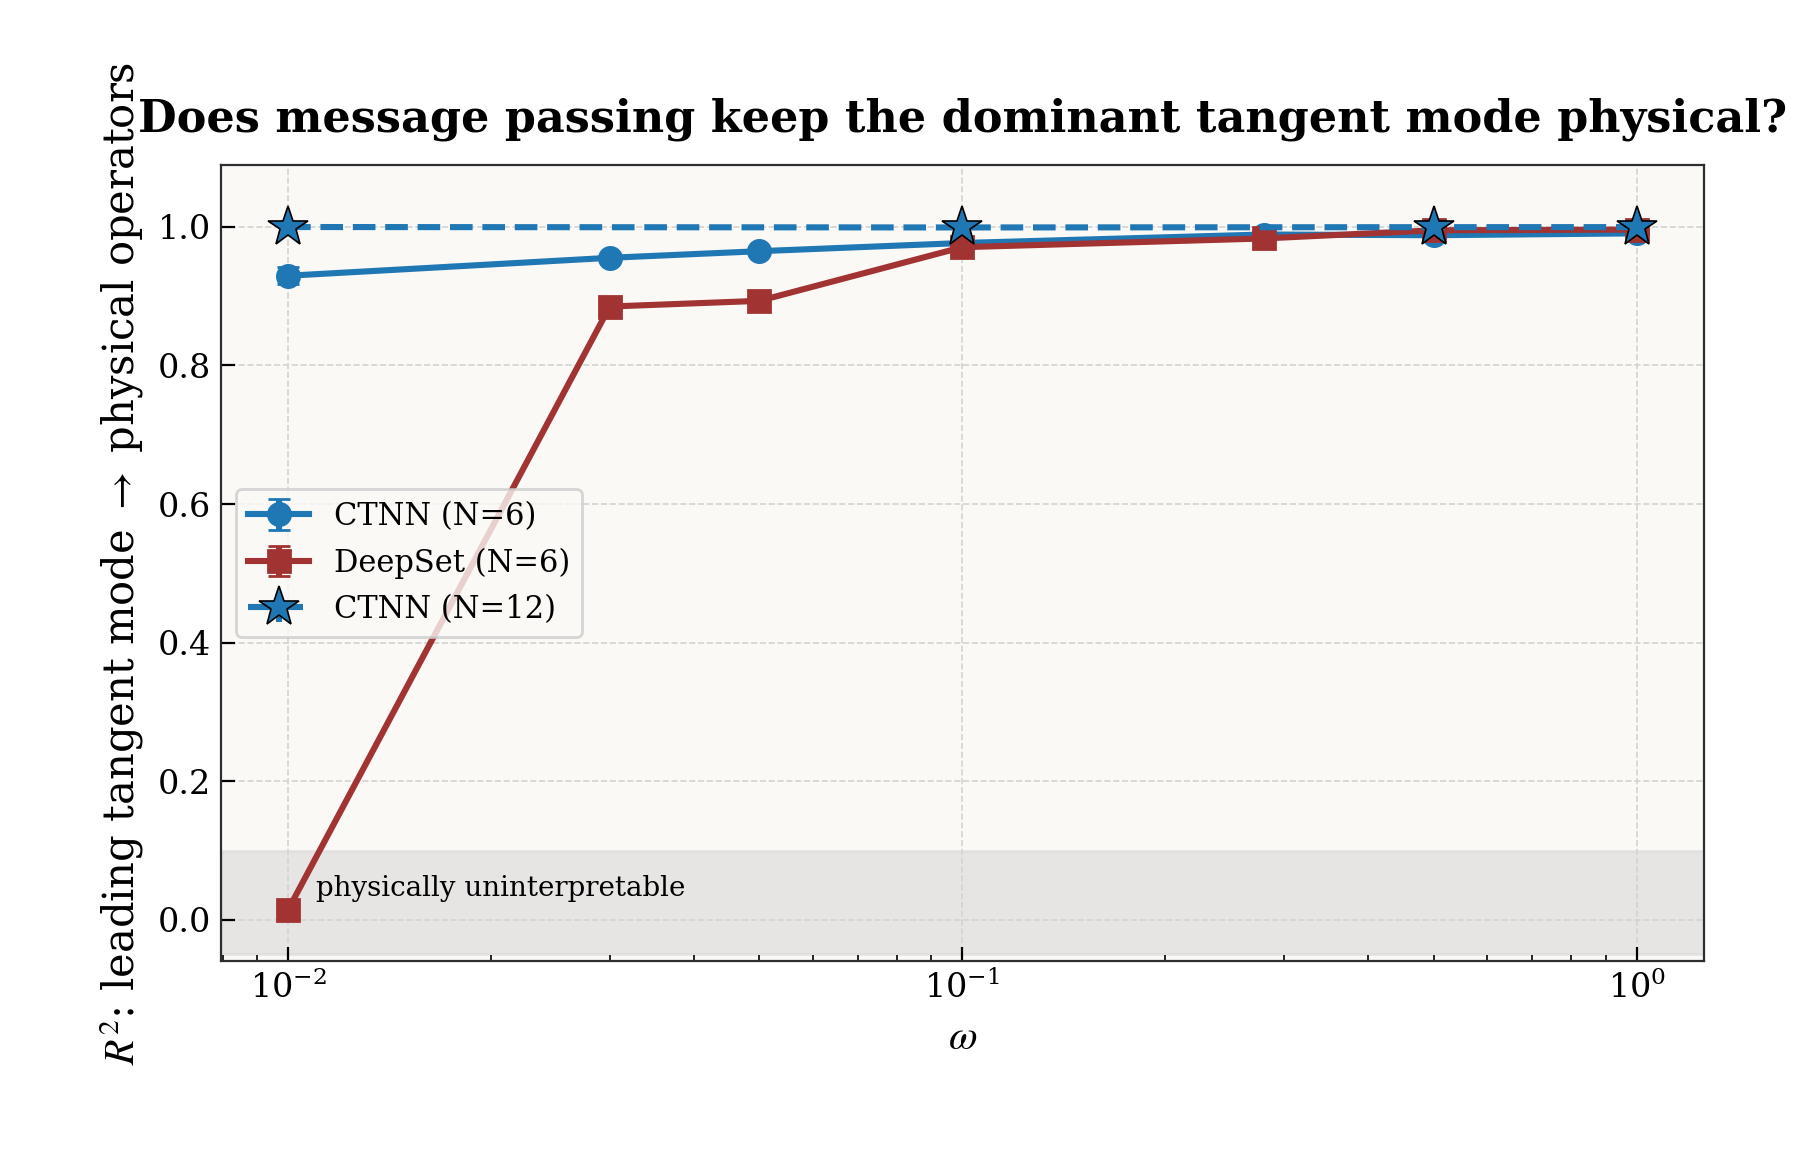
\includegraphics[width=0.9\textwidth]{mode_naming_scan.png}
  \caption[Leading-mode fit to the selected operator dictionary]{$R^2$ of the correlator's
  leading tangent-kernel eigenmode against the selected four-operator dictionary,
  seed-averaged over well-trained checkpoints. The CTNN retains a high dictionary fit across
  the grid; the DeepSet fit falls at weak confinement. No random-dictionary null or held-out
  fit was run, so this is a relative comparison. Three seeds at $\omega=0.01$.}
  \label{fig:mode-naming}
\end{figure}

\paragraph{The dominant mode is not the tangent space.} Figure~\ref{fig:mode-naming} scores
the \emph{dominant} eigenmode against the dictionary; Fig.~\ref{fig:nonphys} asks where the
eigenvalue-weighted mass of the leading modes \emph{as a whole} lies. A network can place its
largest mode squarely inside the dictionary and spend most of the rest outside it, which is
what the separable network does---so the leading-mode score is generous to it. At $\omega=1$
it has the slightly higher leading-mode fit ($R^2\approx0.996$ against $0.991$), with
energies identical to four figures. Write the
eigenvalue-weighted fraction of the top tangent modes lying \emph{outside} the
selected-operator span as the \emph{dictionary-orthogonal tangent mass}. The DeepSet carries a large
excess at \emph{every} confinement---$0.44$ against the CTNN's $0.06$ at $\omega=1$, a gap of
$\sim\!0.3$--$0.5$ that persists from the strongly-confined limit down to the crystal
(Fig.~\ref{fig:nonphys}). Thus the separable network can reach the same energy while leaving
nearly half its tangent weight along directions the selected dictionary does not resolve.
Those directions are not necessarily unphysical; the result is only that these four
operators account for one tangent space more completely than the other. Nor is this merely a
consequence of the CTNN's smaller $d_{\mathrm{eff}}$: toward the Wigner regime the two
effective dimensions converge to ${\sim}3.7$ while the dictionary gap persists. At $N=12$
the contrast is stronger still: the CTNN's dictionary-orthogonal mass stays
$\lesssim\!0.02$ across $\omega$, while a matched DeepSet trained to $+0.2\%$ sits at
$\approx\!0.77$ at $\omega=1$.

\begin{figure}[htbp]\centering
  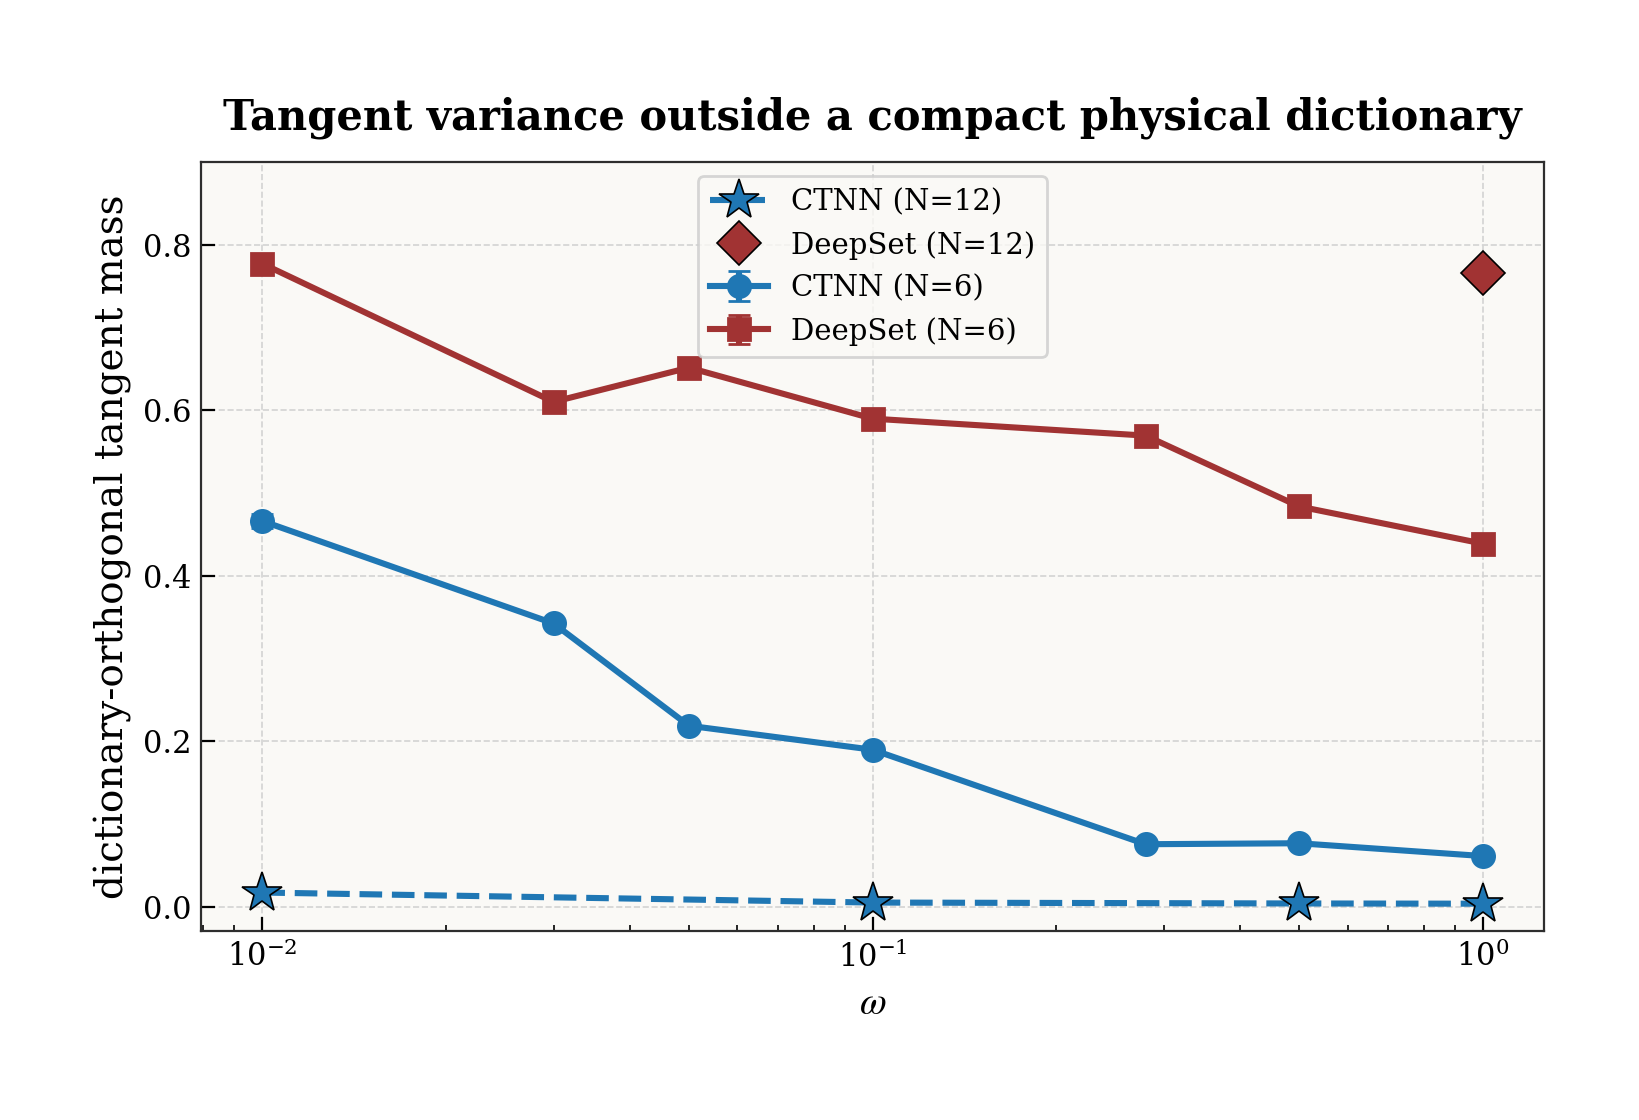
\includegraphics[width=0.85\textwidth]{nonphys_mass.png}
  \caption[Dictionary-orthogonal tangent mass against $\omega$]{Dictionary-orthogonal
  tangent mass---the eigenvalue-weighted tangent variance outside the span of the selected
  four-operator dictionary---against
  $\omega$. At $\omega=1$, where the two correlators agree in energy to $0.001\%$, the DeepSet
  places $44\%$ of its tangent variance outside the dictionary and the CTNN $6\%$; the excess
  persists at every $\omega$.}
  \label{fig:nonphys}
\end{figure}

\subsection{The backflow: rank collapse and its absence}
\label{sec:kernel-q1b}

The contrast is sharper in the backflow, but the comparison is less controlled. The
correlator, data, training protocol and optimiser are shared; capacity, coordinate
preprocessing and centre-of-mass projection are not (\S\ref{sec:bf-init}). At the production
width the copresheaf network has $182$k parameters and the conventional network $51$k, and
no matched pair was trained. The results therefore compare the archived implementations,
not message routing alone.

At $\omega=1$ both implementations reach reference quality, but they diverge as the trap
weakens (Table~\ref{tab:bf_energies}). The CTNN backflow stays within $0.01$--$0.12\%$ across
all $N$ and $\omega$, whereas the conventional backflow reaches $+0.58\%$ at
$N=6,\omega=0.01$ and $+0.69\%$ at $N=20,\omega=0.01$, about six times the CTNN error there.

\begin{table}[htbp]\centering
\caption{Relative energy error (\%) of the two backflow architectures, seed-averaged.}
\label{tab:bf_energies}
\begin{tabular}{l|cc|cc|cc}
\hline
 & \multicolumn{2}{c|}{$N=6$} & \multicolumn{2}{c|}{$N=12$} & \multicolumn{2}{c}{$N=20$}\\
$\omega$ & CTNN & conv & CTNN & conv & CTNN & conv \\
\hline
1.0  & $-0.03$ & $+0.06$ & $-0.01$ & $+0.04$ & $+0.06$ & $+0.07$ \\
0.1  & $-0.05$ & $+0.16$ & $+0.01$ & $+0.16$ & $+0.02$ & $+0.18$ \\
0.01 & $-0.04$ & $+0.58$ & $-0.01$ & $+0.54$ & $+0.12$ & $+0.69$ \\
\hline
\end{tabular}
\end{table}

\paragraph{How component-level numbers are read.}
\label{sec:synthesis}
Energy and $\Var(E_L)$ are state-level quantities; the backflow's rank, displacement
magnitude and component-wise $d_{\mathrm{eff}}$ are not. Because the correlator and backflow
can substitute for one another, these component-level diagnostics record the training route
as well as the state it reached.

This distinction matters here. An earlier rank collapse under joint, from-scratch training
affected both architectures, moved with the seed and carried no energy penalty. The collapse
reported below occurs under the staged protocol, affects only the conventional backflow, is
seed-robust where replicated and accompanies an energy loss. The energetic change makes it
more than a component-level curiosity.

We define the \emph{backflow rank} as the participation ratio of the displacement field
$\Delta\mathbf{x}$: the effective number of independent directions along which the backflow
moves the electrons.

The columns of Table~\ref{tab:bf_rank} have different ceilings: $2N-2$ for the copresheaf
network, which projects out the mean displacement, and $2N$ for the conventional network.
Their absolute levels are therefore not directly comparable. The change with confinement is.
At $\omega\ge0.1$ the conventional field remains near its ceiling; at $\omega=0.01$ it
collapses to rank~$1$ for $N=6$, $12$ and $20$, while the CTNN field remains near full rank.
The tangent dimension changes in the same direction, growing from ${\sim}4$ to ${\sim}10$
for the CTNN and falling from ${\sim}6$ to ${\sim}1$ for the conventional backflow. The
rank-one result is reproduced by both seeds at $N=6$ and $N=12$; the $N=20$ value is from a
single re-run. Because the conventional field retains a centre-of-mass component, the
rank-one endpoint cannot yet be identified with a relative collective mode.

\paragraph{What the comparison supports.} The core observation is simple: in the Wigner
regime the conventional implementation collapses to a rank-one displacement field and its
energy degrades, whereas the CTNN implementation does neither. The cause is not isolated.
The conventional network is a third the size, only the CTNN scales its inputs by
$\sqrt{\omega}$, and only the CTNN removes the mean displacement. The same conventional
network works above the Wigner regime, so the failure is confinement-dependent, but that
does not distinguish capacity, preprocessing and architecture.
Tables~\ref{tab:bf_energies} and~\ref{tab:bf_rank} therefore describe the production
implementations used in Chapter~\ref{ch:results}; they are not an architecture ablation.

\begin{table}[htbp]\centering
\caption[Backflow displacement rank (participation ratio)]{Backflow displacement rank
(participation ratio), evaluated on the field returned by each network. The ceilings are
$2N-2$ ($10/22/38$) for the copresheaf network and $2N$ ($12/24/40$) for the conventional
one, so compare the collapse rather than the absolute levels. The networks are not
capacity-matched ($182$k against $51$k). Entries are two-seed means except at $N=20$,
$\omega=0.01$, which is a single re-run whose per-run rank artefacts were not retained.}
\label{tab:bf_rank}
\begin{tabular}{l|cc|cc|cc}
\hline
 & \multicolumn{2}{c|}{$N=6$} & \multicolumn{2}{c|}{$N=12$} & \multicolumn{2}{c}{$N=20$}\\
$\omega$ & CTNN & conv & CTNN & conv & CTNN & conv \\
\hline
1.0  & $8.8$ & $10.4$ & $20.8$ & $22.2$ & $36.9$ & $35.4$ \\
0.1  & $7.7$ & $10.4$ & $18.2$ & $21.7$ & $33.8$ & $37.6$ \\
0.01 & $9.8$ & $\mathbf{1.0}$ & $20.8$ & $\mathbf{1.0}$ & $35.2$ & $\mathbf{1.0}$ \\
\hline
\end{tabular}
\end{table}

\paragraph{Pricing each component by deletion.} We next ablate components on a common probe
drawn from the full model's $|\Psi|^2$. Holding the configurations fixed isolates the change
in the kinetic term when a component is removed. It does not give the energy of a relaxed
ablated state, so these numbers rank local contributions rather than energetic costs.

(i) On this probe the \textbf{backflow's share shrinks and the Jastrow messages' share grows}
as the trap weakens. Deleting the backflow costs $+5.6\%$ at $\omega=1$ and $+1.4\%$ at
$\omega=0.1$, but only $+0.013$--$0.017\%$ at $\omega=0.01$ (three seeds), while deleting the
Jastrow messages runs the other way: $+3.9\%$ at $\omega=1$ rising to $+9$--$15\%$ at
$\omega=0.01$. A variational deletion on separately sampled production-width networks gives
the opposite trend: removing the message-passing backflow costs $0.5\%$ at $\omega=1$,
$1.0$--$1.2\%$ at $\omega=0.1$ and $1.9$--$2.0\%$ at $\omega=0.01$. The methods and networks
differ, and the division of correlation between components is route-dependent, so neither
result establishes a physical migration of relational work from nodes to amplitude. The
conclusion that survives is:

(ii) \textbf{Within the backflow, the transport maps \emph{are} the displacement}: zeroing
the inter-particle transport maps ($\rho_{v\to e},\rho_{e\to v}$) perturbs
$\Delta\mathbf{x}$ by as much as deleting it outright---the mean
$|\Delta\mathbf{x}_{\mathrm{abl}}-\Delta\mathbf{x}|$ is comparable to the mean
$|\Delta\mathbf{x}|$ at every $(N,\omega)$. The displacement therefore comes primarily from
the transported messages, not the per-particle path. Both architectures use relative
coordinates, but the conventional backflow aggregates one round of pairwise messages per
particle, whereas the CTNN maintains an explicit edge state across the graph. Empirically,
the former does not sustain a high-rank displacement field at the crystal; the latter
does, and its transport maps carry almost the entire displacement.

\begin{figure}[htbp]\centering
  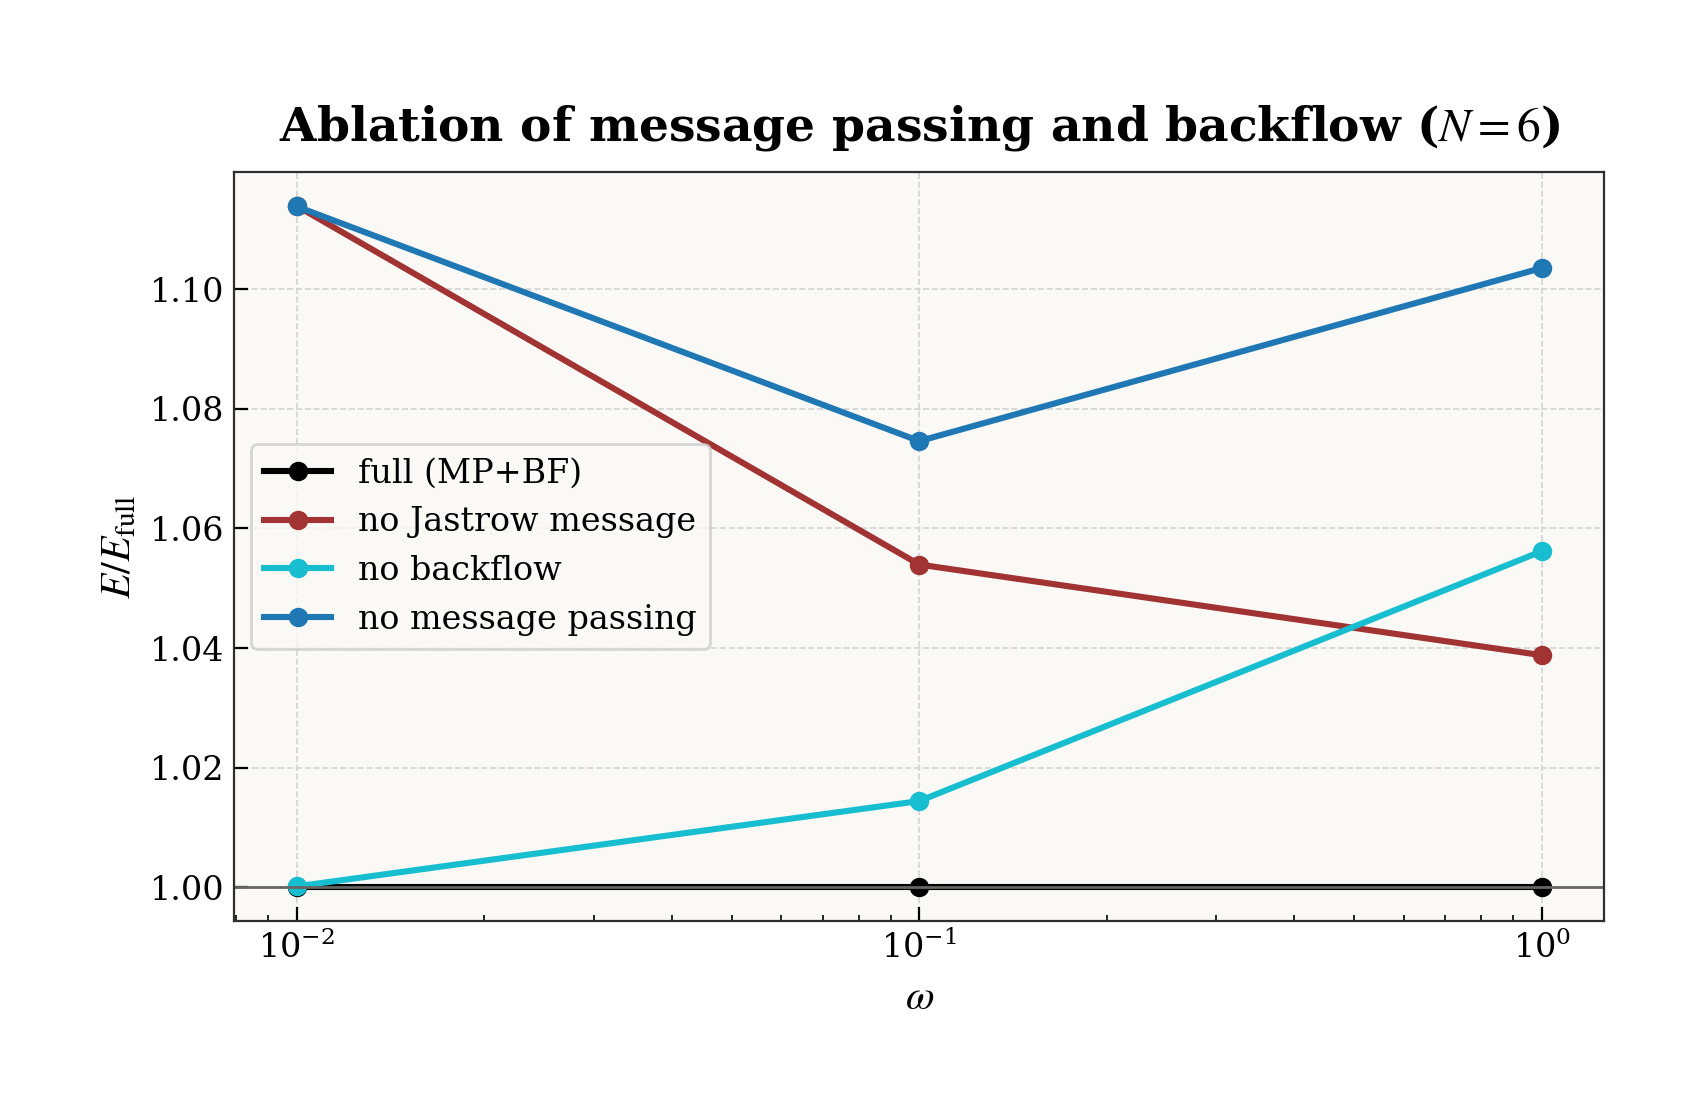
\includegraphics[width=0.85\textwidth]{message_ablation.png}
  \caption[Fixed-measure ablation cost of each component]{The \emph{fixed-measure
  instantaneous ablation cost} of each component (trained networks, $N{=}6$). Configurations
  are drawn once from the full model's $|\Psi|^2$ and every arm is re-evaluated on them, so
  $\Delta E_{\rm probe}/E_{\rm full}$ is the change in the kinetic term when a component is
  switched off, not the energy of a retrained network. Cyan: backflow removed; dark red:
  Jastrow messages removed; blue: all message passing removed. The curves cross near
  $\omega\approx0.4$. The trend reverses when the ablated production-width networks are
  evaluated variationally on their own samples (text).}
  \label{fig:q1b-ablation}
\end{figure}

\subsection{Evidence consistent with a common relational bottleneck}
The two effects may share a cause in how relational information is routed. The separable
correlator pools independently encoded pairs, and the conventional backflow aggregates one
round of pairwise messages; neither retains a transported edge state. The CTNN variants do.
To test whether the two diagnostics move together, we retained the conventional backflow in
both arms, changed the correlator family, retrained each arm and followed the sweep in
$\omega$.

The backflow's failure boundary moves with the correlator. With a separable correlator the
two give way together near $\omega\approx0.05$: correlation-hole capture falls from $0.68$
to $0.07$ and the displacement rank from ${\sim}10$ to $1$ across the same step. With a
message-passing correlator both hold half a decade further, to $\omega\approx0.01$
(Fig.~\ref{fig:q1-unify}).

Each arm is a separately trained model, and the correlators differ in primitive features as
well as routing. The co-movement is therefore consistent with a shared relational bottleneck,
but does not exclude feature scaling, optimisation path or capacity as common causes.

\begin{figure}[htbp]\centering
  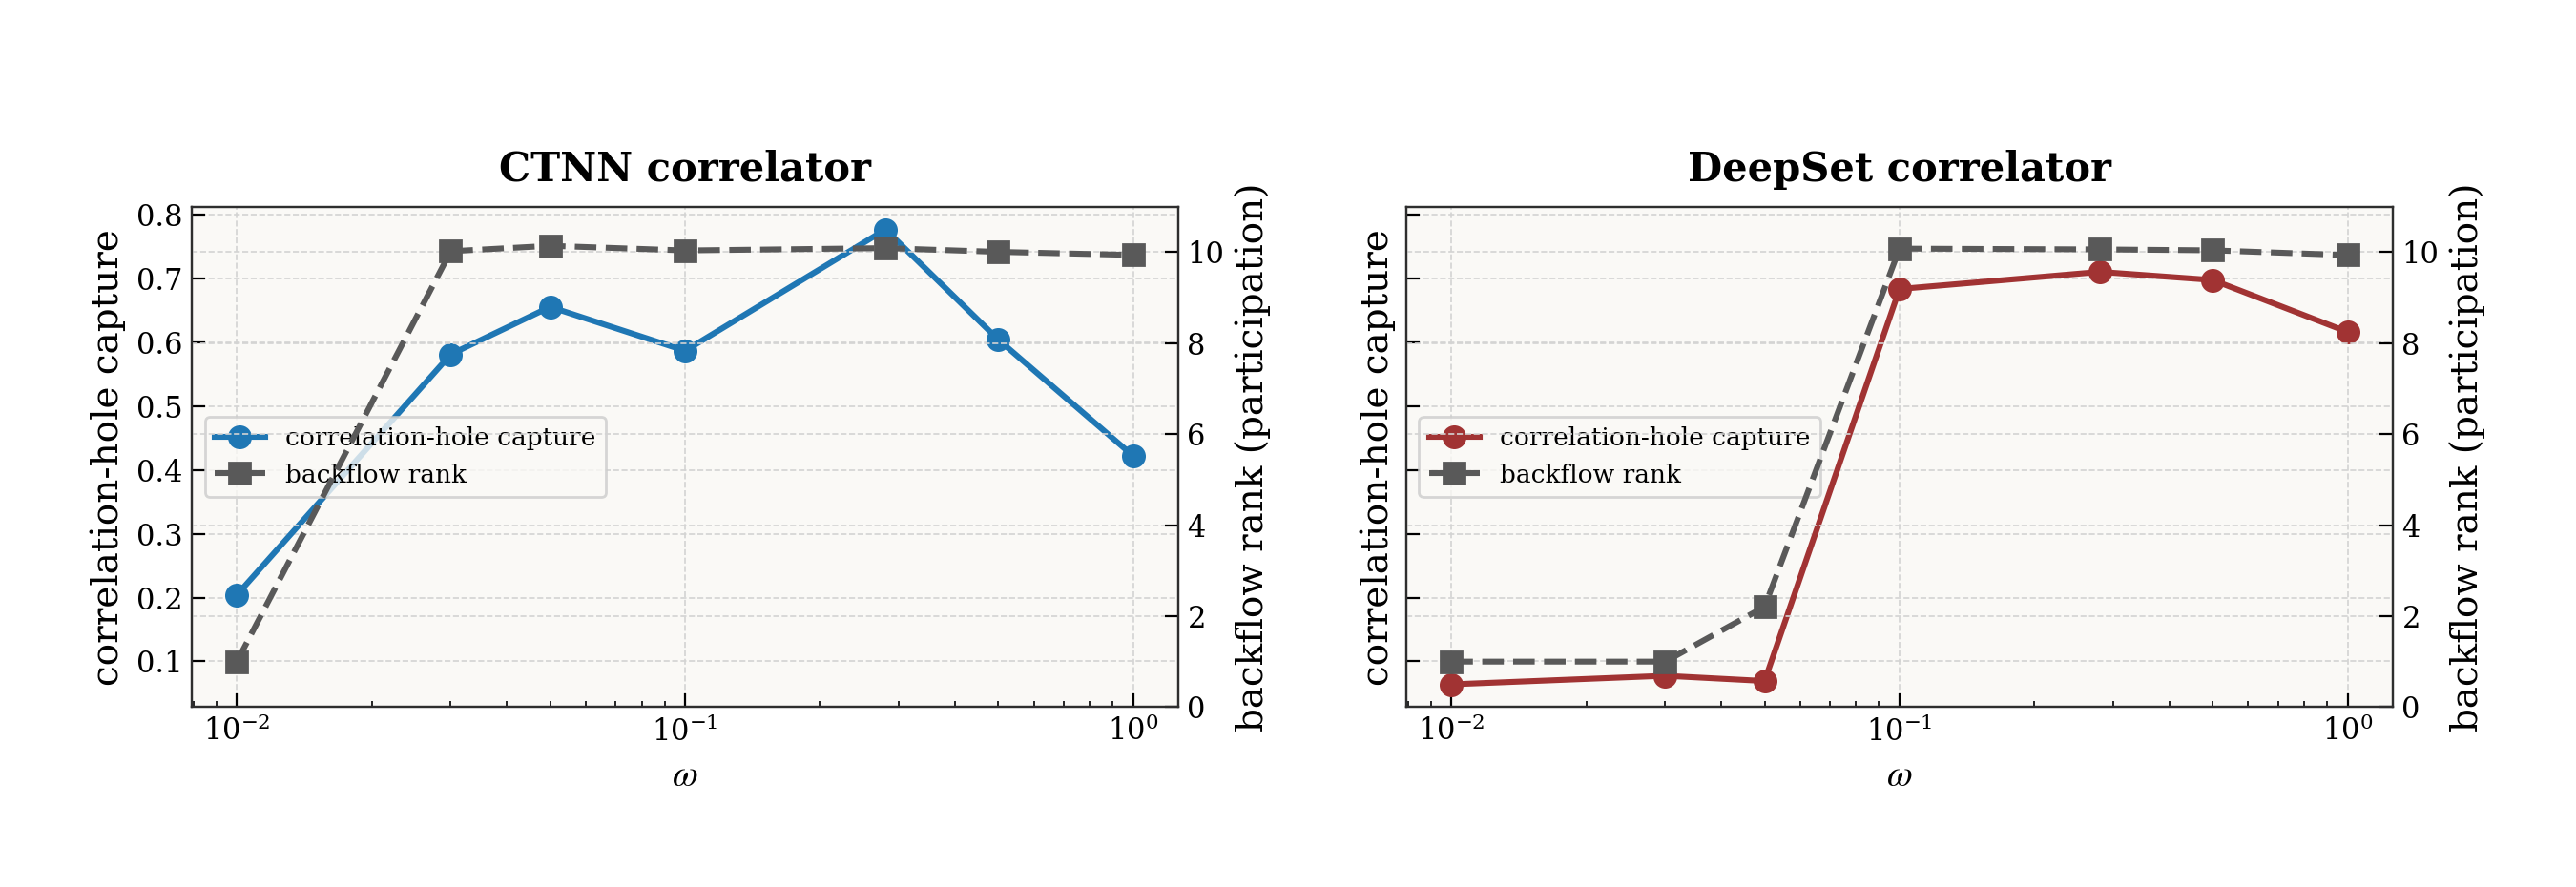
\includegraphics[width=\textwidth]{q1_unification.png}
  \caption[Correlator dictionary fit and backflow rank across confinement]{Correlator
  dictionary fit and backflow displacement rank for $N=6$, with the conventional backflow
  used in both arms. For each correlator family, the
  correlation-hole capture (left axis) and the backflow displacement rank (right axis) give way
  at the same $\omega$: $\omega\!\approx\!0.05$ for the DeepSet, $\omega\!\approx\!0.01$ for the
  CTNN. The co-movement is consistent with a shared bottleneck, but the correlator features
  are not otherwise matched.}
  \label{fig:q1-unify}
\end{figure}
\FloatBarrier

% =====================================================================
\subsection{What the trained representation looks like}
\label{sec:kernel-repr}

One descriptive result belongs beside these controlled comparisons. Examining a single
high-quality trained solution shows the correlator occupying a feature space of one to three
effective dimensions across the entire grid and never expanding: at $\omega=10^{-3}$, where
the real-space density has developed rings and discrete occupancies, the latent rank is no
larger than at $\omega=1$. What changes across the crossover is which branch the leading axis
draws on, not how many axes there are. The displacement field is the opposite kind of object,
spanning nearly all the spatial directions available to it and leaving the correlator's
feature geometry almost unperturbed.

These are component-level measurements on one run. They are gauge-like---the correlator and
backflow are partial substitutes, so the division of labour between them records the training
route as much as the state---and no architectural conclusion above depends on them. They are
recorded because a low effective covariance rank is not what one would predict for a
state whose real-space structure is this elaborate, and because the reorganisation happens
near $\omega\approx0.1$, the same confinement at which the energy partition crosses over
(\S\ref{sec:wigner-energy}). Whether that coincidence reflects one mechanism or two we cannot
say from a single run. Appendix~\ref{app:representation} gives the full analysis.

\medskip
\noindent The implemented correlator families differ before their energies do. Under the
parametrisations used here, the CTNN concentrates its Fisher weight in fewer directions at
strong confinement and is better described by the selected dictionary; its local-energy
variance is also lower by factors of $1.2$ to $3.4$. In the backflow sweep, the conventional
implementation collapses to rank one and loses half a percent where the CTNN does not. Since
the comparisons are not matched in every feature, scale and constraint, these are findings
about the archived implementations rather than message passing alone; their co-movement
motivates the shared-bottleneck hypothesis. The state-level result is the variance:
correlators that agree in energy to four figures but differ in variance have reached
different \emph{states}. Their overlap was not measured, so the variance does not quantify
that difference.

\section{Conditioning and the sampling measure}
\label{sec:kernel-cond}
\label{sec:kernel-q2}

Two design choices remain, and the tangent geometry connects them. One asks what a
natural-gradient step buys over a diagonal one. The other asks what changes when the loss is
defined by an analytic proposal instead of by $|\Psi|^2$. They are the same question twice
over: stochastic reconfiguration inverts the metric $S$, and the sampling measure is what
builds $S$ in the first place.

\subsection{Natural-gradient preconditioning}
Stochastic reconfiguration preconditions the gradient by the inverse QGT,
$\btheta \leftarrow \btheta - \eta\, S^{-1}\nabla_{\btheta} E$; geometrically it \emph{whitens} the tangent
kernel. At $N=2$ this is exact: the SR step aligns with the imaginary-time direction
to numerical precision. The question is where whitening changes the outcome.

Fixing the ansatz and varying only the optimiser from a common stage-3 base:
\textbf{for $|\Psi|^2$-VMC, SR and Adam are indistinguishable}---exact at $N=2$
(var $\sim\!10^{-9}$), and at $N=6$ the energy gap
$E_{\mathrm{Adam}}-E_{\mathrm{SR}}$ is $\lesssim0.002$ across $\omega$ and both
seeds; in the matched pair at $\omega=1$ the two agree to four decimals in relative error.
\textbf{For weak-form collocation from the same common base, SR is decisive}: there
$E_{\mathrm{Adam}}-E_{\mathrm{SR}}$ is large and positive (e.g.\ $+2.9$ at
$N=6,\omega=1$), and plain Adam does not converge the objective.

This controlled comparison does not conflict with \S\ref{sec:colloc-method}, where Adam is
the production default. With a bare objective and fixed proposal, the collocation gradient
stalls under a diagonal step and SR rescues it. The production pipeline instead controls the
gradient at its source through proposal refitting, oversampling, reward normalisation,
rollback and cascade warm-starting; once these are in place, Adam suffices, although their
individual effects were not isolated (\S\ref{sec:gradient-chain}). Below
$\omega\simeq0.01$, the samples used to build $S$ collapse and SR becomes unstable, so Adam
is the more robust default. Its large speed advantage in our code mainly reflects the
per-sample loop used to construct the score matrix: vectorising that calculation makes it
$25$ times faster at $N=6$ and $82$ times faster at $N=20$
(Appendix~\ref{app:walltime}). The comparison here concerns what SR buys, not what it costs.

A large condition number alone does not explain the difference. Table~\ref{tab:kappa}
reports
$\kappa(S)=\lambda_{\max}/\lambda_{\min}$ measured on the trained states under $|\Psi|^2$
sampling, and it is enormous, $10^{7}$ to $10^{10}$, for \emph{both} architectures and at
every capacity in the ladder, including precisely the models on which Adam and SR agree to
four decimals. Whatever makes SR unnecessary under $|\Psi|^2$ sampling, it is not that the
metric is well conditioned.

\begin{table}[htbp]\centering
\caption[Condition number of the empirical geometric tensor]{Condition number of the
empirical quantum geometric tensor at $N{=}6$, $\omega=1$, measured on each trained state's
own $|\Psi|^2$ samples at fixed batch $B=768$. Since $B<P$, $\lambda_{\min}$ is the smallest
sample-supported eigenvalue and depends on batch size, regularisation and the numerical
threshold; $\kappa$ should therefore be read by order of magnitude. The
$d_{\mathrm{eff}}$ values use the same finite batch rather than the converged common probe of
\S\ref{sec:kernel-q1a}, and are included only to show that $\kappa$ does not track them. Adam
and SR reach the same energy on every row.}
\label{tab:kappa}
\begin{tabular}{llcc}
\hline
architecture & params & $\kappa(S)$ & $d_{\mathrm{eff}}$ \\
\hline
CTNN (seed 1)      & $79.8$k & $6.9\times10^{7}$  & $1.46$ \\
CTNN (seed 2)      & $79.8$k & $5.2\times10^{7}$  & $1.39$ \\
DeepSet (small)    & $20.2$k & $3.2\times10^{9}$  & $3.56$ \\
DeepSet (medium)   & $47.7$k & $3.4\times10^{7}$  & $4.35$ \\
DeepSet (matched)  & $89.4$k & $3.2\times10^{10}$ & $3.61$ \\
DeepSet (large)    & $164$k  & $1.4\times10^{7}$  & $4.76$ \\
\hline
\end{tabular}
\end{table}

For the tested $N=2$ and $N=6$ cases, the data rule out condition number alone. Our working
hypothesis is that SR matters when the tangent metric is anisotropic and still statistically
estimable; a noisy or rank-deficient estimate can make $S^{-1}$ amplify rather than suppress
noise. The instability of CG-SR at ultra-weak confinement is consistent with this account
(\S\ref{sec:colloc-negatives}). The criterion remains a hypothesis because the
collocation-space spectrum was not measured at matched batch size; neither the optimiser
comparison nor the spectrum measurement was extended to $N=12$ or $20$.

% =====================================================================
\subsection{Consequences of the sampling measure}

VMC and importance-sampled collocation use the same Slater--Jastrow--backflow form, but the
reported models are not capacity matched. Their training also changes the loss and its
sampling measure. The following three consequences concern that measure change; they are
not controlled architecture comparisons.
\paragraph{Target sampling aligns the estimator with the metric; a covering proposal does
not.} Sampling from $|\Psi|^2$ makes the estimators of $S$ and of the gradient share the
measure that defines them, so the directions carrying Fisher weight are also the directions
the batch populates. That is an alignment between estimator and objective, not
preconditioning in the sense of applying $S^{-1}$. A fixed covering proposal instead drives
a monotone \emph{ESS collapse} as $N$ and $1/\omega$ grow: at $N=6,\omega=0.01$ the
effective sample size, measured against a converged state, falls to $0.11\%$ of the
batch---about $5$ of the $4096$ retained points---and the gradient estimator is then
degenerate. (Table~\ref{tab:ring-ess} finds $1.5$ for the same mixture against a different
converged checkpoint at the same $(N,\omega)$; at a handful of effective points the ESS is
itself a noisy number, and the two are the same collapse.) In this setting the result
diagnoses severe estimator failure; continued training with the same static proposal does
not address the lost overlap. (Two ESS normalisations appear in this chapter, differing by
the oversampling factor; each figure states which.)

\S\ref{sec:colloc-reliability} below nonetheless reports usable collocation energies at the
same $(N,\omega)$---$+0.22$--$0.26\%$ across three seeds, Table~\ref{tab:reliability}---and
the two situations differ in the sampler and in the quantity being described. The sampler
first: the collapse measured above is for the \emph{static} origin-centred
mixture, while the campaign's robust recipe refits its proposal every $30$ epochs and
oversamples $16\times$. The campaign's \emph{baseline} rows, which keep the static
proposal, are the ones that blow up ($+3.9$ to $+7.2\%$ at $\omega=0.001$). Second, and
more interesting, the two statements are not about the same quantity. The energy stays within a third of a percent while the modulus overlap ceases to be
resolvable---which is the sharpest illustration in this thesis of why energy alone does not
certify a state. We stop short of saying the overlap \emph{is} zero: $\mathcal{S}^2$ is a
ratio estimator built from the same degenerate weights, so at this ESS it reports \emph{unresolved} and not orthogonal.

\begin{figure}[htbp]\centering
  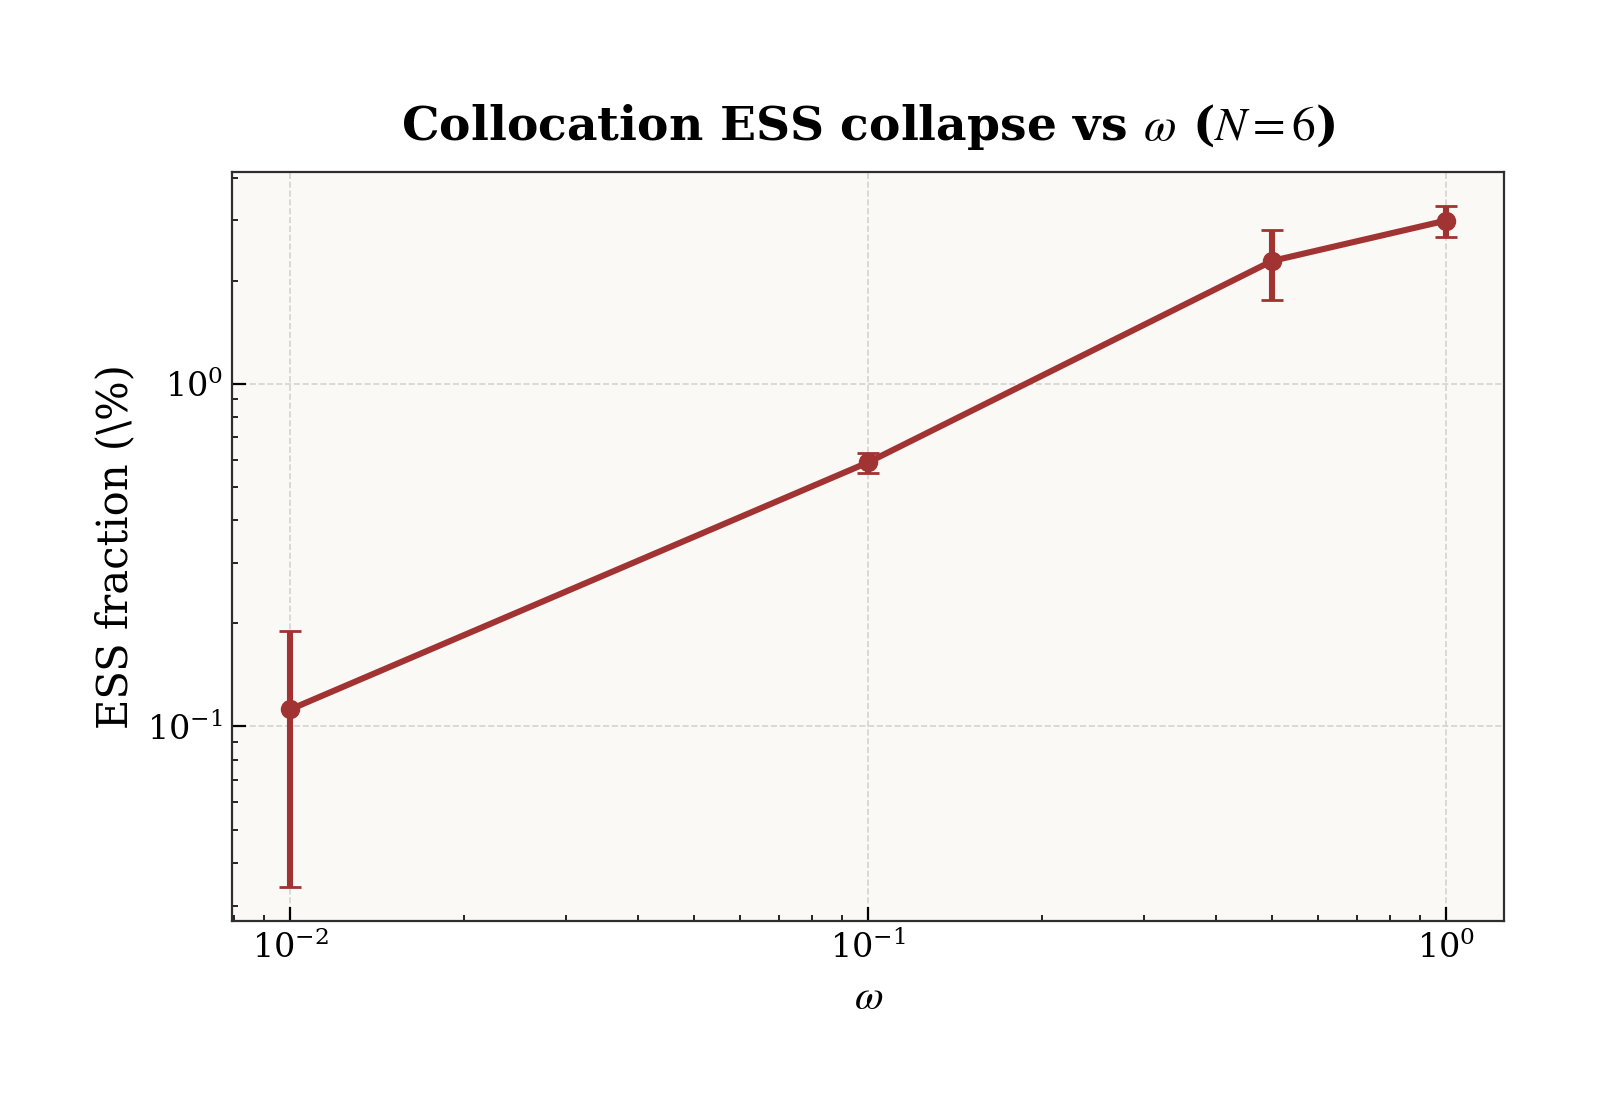
\includegraphics[width=0.8\textwidth]{ess_collapse.png}
  \caption[ESS collapse of the naive collocation proposal]{The naive collocation proposal collapses in the Wigner regime ($N{=}6$). The
  effective sample size (as a percentage of the batch) falls by more than an order of
  magnitude from $\omega{=}1$ to $\omega{=}0.01$, where it reaches $\sim\!0.1\%$---about five
  usable points in a batch of $4096$. This diagnoses proposal--target mismatch for the
  sampled state and motivates the physics-informed ring proposal of
  \S\ref{sec:kernel-q3-frontier}, which is designed to repair it.}
  \label{fig:q3-ess}
\end{figure}

\paragraph{Amplitude agreement degrades with proposal overlap.} We test whether the two
paradigms reach similar wavefunction amplitudes, rather than merely similar energies, using
the symmetric modulus-overlap diagnostic
$\mathcal{S}^2=\langle\Psi_B/\Psi_A\rangle_{|\Psi_A|^2}
\langle\Psi_A/\Psi_B\rangle_{|\Psi_B|^2}$. At $N=2$ the amplitudes agree closely
($\mathcal{S}^2>0.997$ for every $\omega$, both optimisers, both seeds): the paradigm
is efficiency-only, collocation paying $\sim\!5\times$ the variance for essentially the
same amplitude. At $N=6$ they \emph{diverge}: under Adam $\mathcal{S}^2$ falls from $0.85$ at $\omega=1$ to
$0.77$ at $\omega=0.1$ (both seeds), tracking the ESS collapse, and at $\omega=0.01$ the
estimator returns values near zero but is no longer resolved---at an ESS of about five
points it is a ratio of two degenerate importance-weighted averages, and we record it as
\emph{unresolved} rather than as a measured orthogonality. SR partially rescues the
$\omega=0.1$ value ($\mathcal{S}^2\!\approx\!0.95$) but does not close the gap. Weak-form
collocation reaches essentially the same amplitude as VMC at the two-electron anchor. At $N=6$
the amplitudes already differ at strong confinement and become harder to compare as proposal
overlap deteriorates.
In these tests, the route that benefits from SR is also the one that becomes unreliable as
the proposal loses overlap. An adaptive proposal that tracks $|\Psi|^2$ is the next remedy tested in
\S\ref{sec:kernel-q3-frontier}.

\paragraph{Why the collocation energy readout is biased.} For an exact eigenstate the
local energy $E_L=\hat H\Psi/\Psi$ is constant over configuration space, so
$\Var(E_L)\to0$ as the ansatz approaches the ground state---the zero-variance principle,
and the reason $\Var(E_L)$ is a sharp quality measure. That cancellation is a property of
the \emph{full} local energy, in which the kinetic (Laplacian) and potential terms combine
to a constant; it is not a property of the Laplacian term alone. The collocation objective
does \emph{not} discard the Laplacian: it is a score-function (REINFORCE) estimator that
\emph{forms} the full $E_L$ as a detached reward and differentiates only $\log|\Psi|$
(\S\ref{sec:colloc-method}). What it gives up is the \emph{measure}, and three things then spoil the readout, in
increasing order of severity. The estimator is self-normalised, since $|\Psi_\theta|^2$ is
unnormalised, so it carries an $\mathcal O(1/n)$ finite-sample bias that vanishes with sample
size. The tail controls deliberately change the target: tempering $w\to w^\alpha$ and
clipping the log-weights trade bias for variance on purpose, so the estimated quantity is no
longer $\langle E_L\rangle_{|\Psi|^2}$. And, dominant in the regimes that matter,
proposal--target mismatch inflates the variance beyond any affordable sample size
(\S\ref{sec:colloc-reliability}). Importance sampling is not biased merely for being
importance sampling; it is the last two that make the readout unusable as a stopping rule.
The reliable readouts are $\Var(E_L)$ and the modulus overlap, both on $|\Psi|^2$ samples, and
for the same reason no energy reported in this thesis is an importance-sampling estimate:
every one is a Metropolis evaluation of $|\Psi|^2$.

The practical question is therefore how far an analytic proposal can preserve usable
gradient statistics without a Markov chain.

\section{Training with MCMC-free gradient updates}
\label{sec:kernel-mcmcfree}
\label{sec:collocation}

The conditioning story has a practical edge. If the sampling measure is what makes the
metric estimable, then choosing that measure is a design decision, not a fact of nature---and
the obvious thing to try is a measure with no Markov chain in it at all. ``MCMC-free''
refers to the gradient throughout: no configuration entering a parameter update comes from a
chain, but a Metropolis probe still selects checkpoints and certifies the final energy, and
the cascades start from reference-guided pretrained states
(\S\ref{sec:collocation-discussion} states the claim exactly).

\paragraph{Two distinct limits.}
The method encounters proposal degeneracy and failure to transfer a checkpoint between
confinements. The results below separate them.

\emph{The first limit is statistical.} A fixed analytic proposal loses overlap with
$|\Psi_\theta|^2$ as the trap opens; the importance weights grow heavy-tailed; the gradient
estimator comes to be dominated by a handful of draws; the empirical metric becomes
unreliable and preconditioning can then amplify noise. The evidence is consistent with a
sampling limit, and a better proposal moves the observed boundary---from $\omega\approx0.01$ with an
origin-centred mixture to $\omega=0.0035$ with one built out of the measured Wigner
geometry.

\emph{The second limit concerns transfer.} Below $\omega=0.0035$ a stable trained state fails
to survive transfer to a weaker trap even when the sampler is initialised directly on the
correct shell. Diagnostics point to a near-balance between the confining determinant and
the compensating Jastrow, which is disturbed by the $23\%$ change in $\omega$. Correct
shell initialisation alone does not repair the transferred state.
It limits the cascade, which carries trained states down in small steps of $\omega$,
and not for MCMC-free gradient updates as such: started instead from a pretrained checkpoint,
the reliability campaign of \S\ref{sec:colloc-reliability} trains $N{=}6$ at $\omega=10^{-3}$
to within $0.35\%$ of our SR--VMC energy.

\noindent \S\ref{sec:kernel-mcmcfree} documents the proposal-degeneracy evidence;
\S\ref{sec:kernel-q3-frontier} moves that observed boundary and then encounters the transfer
failure.

A Markov chain is what makes neural variational Monte Carlo sequential. Chains must
equilibrate, successive samples are correlated, and mixing times grow with particle number
and with correlation strength. They grow fastest, in other words, exactly where the physics
gets interesting.

Draw the configurations instead from a fixed analytic proposal and reweight them, and the
whole gradient step becomes embarrassingly parallel. The question is what that costs.

Two ways of posing the problem behave very differently, and the difference decides
everything downstream. The \emph{strong form} asks the wavefunction to satisfy the local
Schr\"odinger equation pointwise, minimising the variance of $E_L$ and differentiating
through the Laplacian to do it. The \emph{weak form} uses a score-function (REINFORCE)
gradient in which the Laplacian enters only as a reward and is never differentiated.
Appendix~\ref{app:catch22} shows why this is difficult for a backflow: $E_L$ generally has a
pole at a simple trial node, and differentiating through a node that moves with the
parameters makes the empirical gradient more singular. None of the tested combinations of
sampling, loss and preconditioning improved beyond an error near $0.3\%$. Model sizes were
not matched to production VMC, so the experiment motivates the change of objective without
identifying the objective as the sole cause. Everything below uses the weak form.

Using the same Slater--Jastrow--backflow ansatz form, and with no
Markov chain in any gradient, the weak form comes within about a tenth of a percent of DMC
at strong confinement and within about a third of a percent of our lowest SR--VMC energies
well into the correlated regime for $N\in\{6,12\}$ (Table~\ref{tab:collocation}). The energies are collected here, where the method that
produced them is explained, rather than beside the SR--VMC energies of
\S\ref{sec:energy-overview}: without the failure mechanism of
\S\ref{sec:colloc-reliability} in hand, the pattern of where they hold and where they give
way is not interpretable.

\begin{table}[htbp]
  \centering
  \caption[Energies from MCMC-free gradient training]{Metropolis energies of
  states trained with MCMC-free gradients. Parentheses in the reported-energy column give
  standard errors. For $N{=}6$,
  both the best result and the mean $\pm$ standard deviation of three protocol-controlled
  seeds are shown. The $N{=}2$ and $N{=}12$ rows are single runs; $^{\dagger}$ marks
  continuation runs using the corrected proposal density. References are external where
  available and otherwise the lowest SR--VMC energy, so those deviations measure internal
  agreement. Energies are in effective Hartree.}
  \label{tab:collocation}
  \begin{tabular}{c c c c c c}
    \toprule
    & & & & \multicolumn{2}{c}{relative deviation (\%)} \\
    \cmidrule(lr){5-6}
    $N$ & $\omega$ & Reference & Reported energy & best & mean $\pm$ s.d. \\
    \midrule
    2 & 1.0   & $3.00000$      & $3.00105(44)$  & $+0.035$ & --- \\
      & 0.5   & $1.65977(1)$   & $1.65945(80)$  & $-0.019$ & --- \\
      & 0.1   & $0.44079(1)$   & $0.440944(56)$ & $+0.035$ & --- \\
      & 0.01  & $0.073839(2)$  & $0.073911(11)$ & $+0.098$ & --- \\
      & 0.001 & $0.013778$     & $0.013889(9)$  & $+0.806$ & --- \\
    \midrule
    6 & 1.0   & $20.15932(8)$  & $20.1731(18)$  & $+0.068$ & $+0.082\pm0.014$ \\
      & 0.5   & $11.78484(6)$  & $11.7952(12)$  & $+0.088$ & $+0.098\pm0.009$ \\
      & 0.1   & $3.55385(5)$   & $3.56393(24)$  & $+0.284$ & $+0.293\pm0.009$ \\
      & 0.01  & $0.69036$      & $0.691895(80)$ & $+0.222$ & $+0.244\pm0.020$ \\
      & 0.001 & $0.140832$     & $0.141175(4)$  & $+0.244$ & $+0.282\pm0.059$ \\
    \midrule
    12$^{\dagger}$ & 1.0 & $65.7001(1)$   & $65.7207(17)$  & $+0.031$ & --- \\
       & 0.5   & $39.1596(1)$   & $39.1727(12)$  & $+0.034$ & --- \\
       & 0.1   & $12.26984(8)$  & $12.28361(32)$ & $+0.112$ & --- \\
    \bottomrule
  \end{tabular}
\end{table}

\subsection{The weak-form objective}
\label{sec:colloc-method}
The collocation training used here is exactly the MCMC-free gradient pipeline specified in the
Methods: a weak-form (REINFORCE~\cite{Williams1992-REINFORCE}) objective in which the local energy
enters as a detached reward (\S\ref{sec:method-collocation},
Eq.~\eqref{eq:reinforce-method}), an analytic Gaussian-mixture proposal reweighted to
$|\Psi_\theta|^2$ with ESS / Pareto-$\hat k$ monitoring~\cite{Vehtari2024} and tail
controls (\S\ref{subsec:colloc-proposal}), and---in the Wigner
regime---the physics-informed ring proposal with cascade warm-starting
(\S\ref{subsec:colloc-wigner}). Two methodological findings shape what follows. First, among
the optimisers (\S\ref{sec:sr-stage}), \textbf{Adam} was the robust
default across all regimes, whereas \textbf{CG-SR} converged faster at $\omega\!\ge\!0.1$ but
diverged for $\omega\!\le\!0.01$, where the importance weights collapse. This is consistent
with an unresolved empirical metric, although that metric was not measured there directly.
Second, \textbf{cascade warm-starting}, initialising each confinement from a stable checkpoint at a stronger one, was decisive for reaching the deep-Wigner regime, exploiting
the transfer of correlation structure across $\omega$.


\label{sec:colloc-architectures}
Three ansatz families were tried within this framework. The Jastrow-only and backflow
variants share a Slater--Jastrow core; the neural Pfaffian changes the antisymmetric part.
Their definitions and sizes are in \S\ref{sec:hyperparameters}. The
\textbf{backflow+Jastrow} family produced the best
results at $N{=}6$ and $N{=}12$ and carries every number below. The
\textbf{Jastrow-only} family was the fastest and most robust to train, served as the
initialiser for the backflow runs, and becomes the better choice at $N{=}20$ for the memory
reason of \S\ref{sec:colloc-arch-discussion}. The \textbf{neural
Pfaffian}~\cite{GaoGuennemann2024-NeuralPfaffian}, which replaces the determinant with a
more general antisymmetric form and in principle offers richer nodal topology, reached only
$+0.43$--$0.50\%$ at $N{=}6$, $\omega{=}1$ against $+0.07$--$0.10\%$ for backflow+Jastrow.
Its larger parameter space coincided with noisier importance-sampled gradients, but the
comparison does not separate parameter count, optimisation and nodal flexibility.

\paragraph{Why the weak form is stable where the strong form is not.}
\label{sec:colloc-why-reinforce}

The catch-22 analysis (Appendix~\ref{app:catch22}) identifies a nodal heavy-tail problem for
direct residual training. Near a simple trial node, write
$\Psi_\theta\sim a d_\theta$, $E_L\sim c/d_\theta$ and, for a moving node,
$\partial_\theta\log|\Psi_\theta|\sim1/d_\theta$. A strong squared residual sampled from a
smooth covering proposal is then non-integrable. Differentiating it also propagates through
the Laplacian.

The weak-form estimator does not remove nodal heavy tails, but it reduces the singularity it
must handle and keeps the Laplacian out of the gradient path. Its per-sample energy-gradient
factor scales as $(E_L-E)\partial_\theta\log|\Psi|\sim1/d_\theta^2$; the mean is locally
integrable under $|\Psi|^2\sim d_\theta^2$, although its ideal variance can diverge. This
distinction matches the empirical result: the weak form trains the tested backflows where
direct residual minimisation fails, without establishing that all weak-form estimators are
well behaved near nodes.

The better performance of pure REINFORCE ($\beta{=}0$) over the hybrid
objective ($\beta{>}0$) has a related possible explanation.
The direct weak-form term $\tilde{E} = \tfrac{1}{2}\|\nabla\log|\Psi|\|^2 + V$
is cheaper to evaluate (no Laplacian needed). Averaged under the current
$|\Psi|^2$ measure, it equals the variational energy by integration by parts.
The implemented direct path, however, differentiates $\tilde E(R)$ at retained
samples without the score contribution from the changing sampling measure; $V(R)$
then has no explicit parameter derivative and the update behaves as a kinetic-only
pathwise gradient.
At nonzero~$\beta$, the observed energy oscillations are consistent with a conflict between
this kinetic-only pathwise update and the REINFORCE estimate of the variational gradient.

\subsection{Collocation performance}
\label{sec:colloc-results}

\paragraph{$N{=}6$: within a few tenths of a percent across all~$\omega$.}
For six electrons, collocation training comes close to the reference wherever one exists,
but not to within it. At $\omega\ge0.5$ every run lands $0.07$--$0.10\%$ above DMC, with
evaluation errors of $0.005$--$0.013\%$, so the gap is resolved and several times the
deviation of the SR--VMC route (Table~\ref{tab:energies}). An earlier reading of these runs put
the best of them at $+0.013\%$, statistically consistent with DMC; that number came from a
single $30\,000$-sample evaluation of the best of three seeds, and the independent
re-evaluation shows it to have been the lucky tail of a noisier estimate. At $\omega=0.1$
the robust recipe sits at $+0.29\%$. At the most extreme confinements,
$\omega\in\{0.01,0.001\}$, where the electrons are separated by
${\sim}30$--$120\,a_0^\ast$ (a few oscillator lengths) and no DMC reference is available,
the energies stay within $0.22$--$0.35\%$ of our lowest variational energies; this is
agreement between two independent training paradigms using the same ansatz form, not a certificate
of absolute accuracy.

These results are achieved without any Markov chain in the training gradients.
MCMC enters only outside the gradient loop: a small Metropolis probe periodically selects the
best checkpoint, and the final heavy evaluation certifies the energy.
The training itself uses $4096$ importance-resampled collocation
points per epoch with an oversampling factor of $8$--$16$, so the importance weights need
$32$--$65$k amplitude evaluations per gradient step. The SR route evaluates the amplitude
about as often: its chain runs a hundred Metropolis sweeps of $1200$ walkers per step. What
collocation removes is therefore not evaluations but their sequential dependence and the
equilibration of the chain. Timed per step (Appendix~\ref{app:walltime}), neither is where the
time goes. At $N{=}6$ a production SR--VMC step takes $516$\,s, of which the chain is $8$\,s
and building the SR score matrix one sample at a time is $495$\,s; a collocation epoch takes
$21$\,s. At the same optimiser the two paradigms cost within about ten percent of each other
per step, because the exact-Laplacian local energy dominates both. Per-step cost does not see
burn-in, autocorrelation between successive samples or slow mixing between configurations,
which is where the chain's real cost lies and which we did not measure.

Staged continuation is what makes those budgets pay, and an exploratory run at
$\omega{=}1.0$ shows the effect cleanly: an initial BF+Jastrow joint REINFORCE stage
(900~epochs, $\text{lr}{=}5{\times}10^{-4}$), a low-LR continuation (750~epochs,
$\text{lr}{=}3{\times}10^{-4}$) and a hard-focus stage (500~epochs,
$\text{lr}{=}2{\times}10^{-4}$), each inheriting the previous checkpoint, improve
monotonically through $+0.08\%$, $+0.05\%$ and $+0.010\%$. That run was hand-tuned and is
not among the protocol-controlled numbers of Table~\ref{tab:collocation}; we report it
because it is the observation that put cascade warm-starting into the campaign's robust
recipe (Table~\ref{tab:colloc-variants}).

\paragraph{$N{=}12$: a few hundredths of a percent at strong confinement.}
For twelve electrons, the BF+Jastrow collocation results track DMC
closely at $\omega\ge 0.5$, at $+0.031\%$ and $+0.034\%$ for $\omega{=}1.0$ and $0.5$
(Table~\ref{tab:collocation}), resolved above the reference at evaluation errors of
$0.003\%$. No reliability campaign was run at this size, so these are single continuation
runs and not protocol-controlled in the way the $N{=}6$ rows are.
At $\omega{=}0.1$ the error increases to $+0.11\%$, reflecting the
growing difficulty of importance sampling in 24~dimensions at weak
confinement.
The ESS at $\omega{=}0.1$ is typically $5$--$15$ per epoch
(out of $4096$ kept points), indicating that the Gaussian mixture
proposal still maintains usable overlap with~$|\Psi|^2$.

Attempts to extend to $\omega\le 0.01$ at $N{=}12$ were
unsuccessful: both direct starts and cascade warm-starts from
$\omega{=}0.1$ failed to converge, with the ESS collapsing to~$1$
and the rollback mechanism rejecting all gradient updates.
This marks the boundary of the current collocation approach for
$N{=}12$.

\paragraph{$N{=}20$ exposes an implementation-level memory--sampling trade-off.}
Twenty electrons in two dimensions push the tested collocation pipeline against its memory
limit. The backflow's edge-feature tensor scales as
$\mathcal{O}(N^2 h_{\mathrm{bf}})$, which at $N{=}20$ forces the hidden dimension, the
collocation budget or the oversampling factor down far enough to degrade the gradient---so
far that a Jastrow-only ansatz, freed of that cost, trains better than the backflow ansatz it
should in principle beat. These runs show a limit of the tested allocation, not that the
architecture has a conceptual $N{=}20$ boundary. The results are reported in
Appendix~\ref{app:postcatch22:frontier}.

\subsection{Ablations and failed variants}
\label{sec:colloc-negatives}

Most of the method space we explored did not work. The failures are reported here beside
the successes because they narrow the useful design space and expose assumptions that the
successful recipe alone would leave implicit. The table records the observed outcome and
the interpretation supported by the available diagnostics.

\begin{table}[htbp]\centering
\caption[Outcomes of tested collocation variants]{Outcomes of tested collocation variants. Errors are relative to
the reference of Table~\ref{tab:collocation}. The three marked $\dagger$ are taken up in
prose below; the rest are recorded for completeness.}
\label{tab:colloc-variants}
\small
\setlength{\tabcolsep}{5pt}
\renewcommand{\arraystretch}{1.15}
\begin{tabular}{@{}p{0.24\linewidth} p{0.17\linewidth} p{0.51\linewidth}@{}}
\toprule
Attempt & Outcome & Interpretation \\
\midrule
Pure REINFORCE ($\beta{=}0$) over the hybrid objective
  & adopted
  & The direct path omits the sampling-measure score contribution; at
    $\beta>0$ it contributes a kinetic-only pathwise gradient that conflicts with REINFORCE,
    and the two gradients oscillate against each other. \\
Cascade warm-start from higher $\omega$
  & essential
  & Cold starts never converged at $\omega{=}0.01$ for $N\ge6$. Cascading from
    $\omega{=}0.1$ cut the initial error from ${\sim}30\%$ to ${\sim}5\%$ and made
    $+0.15\%$ reachable in ${\sim}1000$ epochs. \\
ESS-adaptive oversampling with instability rollback
  & essential
  & Raises the proposal budget when overlap degrades and reverts on energy spikes.
    Without both, $\omega{=}0.001$ diverged within a few hundred epochs. \\
CG-SR below $\omega\simeq0.01$ $\dagger$
  & abandoned
  & $+4$--$36\%$ against $+0.15$--$0.24\%$ from Adam, coincident with severe importance
    degeneracy; the metric was not measured directly in this regime. \\
Langevin proposal refinement $\dagger$
  & abandoned
  & Worse in every configuration tested ($+153\%$ against $+5.7\%$ at $N{=}20$,
    $\omega{=}0.1$). The weights are computed against a proposal the samples have
    stopped following; see below. \\
Finite-difference residual loss
  & abandoned
  & $+0.22\%$ at $N{=}6$, $\omega{=}1$ against $+0.010\%$ from REINFORCE. Sensitive to
    the step size and to noise in the Laplacian estimate. \\
Neural Pfaffian ansatz~\cite{GaoGuennemann2024-NeuralPfaffian}
  & abandoned
  & $+0.43\%$ at $N{=}6$, $\omega{=}1$, forty times the BF+Jastrow error. The larger
    parameter space coincides with noisier gradients; size, optimisation and nodal
    flexibility are not separated. \\
Backflow at $N{=}20$ $\dagger$
  & abandoned
  & $+18\%$ against $+1.32\%$ for Jastrow-only under a memory-forced capacity and sample
    reduction; see \S\ref{sec:colloc-arch-discussion}. \\
\bottomrule
\end{tabular}
\end{table}

\paragraph{Why CG-SR becomes unreliable at weak confinement.}
CG-SR gave the fastest convergence and the best final energies at $\omega\ge0.1$, and
then failed outright below it. Ill-conditioning is a plausible part of the explanation: at
weak confinement, parameters controlling short-range correlation and the orbital envelope
act on scales separated by $1/\sqrt{\omega}$. The Fisher matrix
$F_{ij}=\EE[\partial_i\log|\Psi|^2\,\partial_j\log|\Psi|^2]$ has eigenvalues spanning
many orders of magnitude in the measured VMC case, although it was not measured under the
collocation distribution at the failed points.

Ill-conditioning alone does not account for the failure, because anisotropy is what
makes natural gradients useful in the first place; a well-conditioned metric is one Adam
handles unaided. A plausible additional limit is estimation: $F$ is built from
importance-resampled points, and when the ESS is low a handful of high-weight samples
dominate it. This can leave the empirical matrix noisy and rank-deficient. Tikhonov damping
stabilises the inversion but also suppresses curvature information.

This suggests three regimes. Where the metric is well conditioned, SR may be unnecessary.
Where it is anisotropic and still estimable, SR can be valuable. And where
importance-sampling collapse makes the empirical metric unreliable, inverting it
can amplify estimation noise. The failures above are consistent with the third regime, but
do not establish the three-way classification. The practical implication is about the
estimator rather than the curvature: a second-order method should check that the metric it
inverts is statistically resolved at the sample sizes in use.

\paragraph{Why pushing the samples uphill makes things worse.}
\label{sec:colloc-langevin-discussion}
Langevin refinement was motivated by an intuition that is hard to argue with. If the
Gaussian proposal overlaps $|\Psi|^2$ poorly, evolve the samples up the score
$\nabla_{\mathbf R}\log|\Psi|^2$ for $K$ steps before reweighting, and the overlap should
improve. It failed in every configuration tested, and the reason is standard in the MCMC
literature and easy to miss in an importance-sampling setting.

The weights $w_i=|\Psi(\mathbf R_i)|^2/q(\mathbf R_i)$ are valid only if the
$\mathbf R_i$ came from $q$. After $K$ steps from an out-of-equilibrium start the samples
follow some intermediate $\tilde q$ that depends on $K$ and $\varepsilon$, while the
weights still divide by $q$. The resulting bias is not noise. It pushes the wavefunction
toward the regions the Langevin dynamics favours, which moves $\tilde q$ further the same
way, and the loop closes on itself---which is what the $+153\%$ in the table is. Ten to
twenty steps in $Nd{=}40$ dimensions do not equilibrate. Fixing it means running to
equilibrium, adding a Metropolis--Hastings step, or computing annealed weights along the
non-equilibrium path. The first two are MCMC under another name; the third costs enough
to forfeit the advantage that made the route attractive.

\paragraph{A common reading of the failures.}
Four failures---CG-SR, Langevin refinement, the larger Pfaffian and the $N{=}20$
backflow---are compatible with one finite-sample account. Natural gradients need an estimate of the metric.
Langevin needs samples that have actually equilibrated. A larger parameter space needs a
correspondingly better-resolved gradient. The experiments do not isolate this account from
model and optimisation differences, except that the Langevin variant has a known proposal--weight
mismatch. Section~\ref{sec:colloc-reliability} therefore follows the measurable quantities
from proposal overlap to final evaluation without assigning every failure a unique cause.

\subsection{Reliability analysis: gradient-quality diagnostics}
\label{sec:colloc-reliability}

The results in Table~\ref{tab:collocation} report the \emph{best} energies
obtained by collocation training, selected from multiple runs on different
seeds.
A natural question is whether these results are \emph{typical} or whether
they reflect rare fortunate outcomes from a high-variance process.
This subsection reports a systematic 30-run reliability campaign designed
to answer that question and test how proposal overlap, gradient noise and final accuracy
move together.

\subsubsection{Experimental design}

All runs use the BF+Jastrow ansatz (${\sim}49\text{k}$ parameters)
initialised from the same pretrained checkpoint.
The grid is $N{=}6$ across
$\omega\in\{1.0,\,0.5,\,0.1,\,0.01,\,0.001\}$ with three random
seeds per cell (42, 137, 314), giving $5\times 2\times 3 = 30$ runs.
Two training recipes are compared head-to-head:

\begin{itemize}
\item \textbf{Config~A (baseline):} Adam optimiser with
  $\text{lr}{=}5{\times}10^{-4}$, $\text{lr}_{\text{jas}}{=}5{\times}10^{-5}$,
  4096 collocation points, $8{\times}$ oversampling, local-energy
  clipping at $5\sigma$, no reward normalisation, no rollback, fixed
  Gaussian mixture proposal (Eq.~\eqref{eq:colloc-proposal}).

\item \textbf{Config~B (robust):} Identical to Config~A plus four
  stabilisation mechanisms: $16{\times}$ oversampling (doubling the
  proposal budget), reward normalisation (standardising the REINFORCE
  reward to zero mean and unit variance before the gradient step),
  instability rollback (reverting to the previous checkpoint when the
  energy jumps exceed $3\sigma$, with learning-rate decay of $0.95$),
  and an adaptive Gaussian mixture proposal (8 GMM components refitted
  every 30 epochs to track the evolving $|\Psi|^2$).
\end{itemize}

All runs train for 1200 epochs.
A $20\,000$-sample Metropolis probe of $|\Psi|^2$ every 50 epochs selects the checkpoint, and
the selected checkpoint was evaluated at the end of training by a fresh $30\,000$-sample
Metropolis run. Every number below is instead an independent re-evaluation of that saved
checkpoint, made for this revision with four separately seeded chains of $102\,400$ samples
each and blocking; it reproduces the original evaluations within their errors on average,
but not the best-of-three values selected on them (\S\ref{sec:gradient-chain}).

\subsubsection{Main results}

Table~\ref{tab:reliability} gives all thirty runs, three seeds per cell.

\begin{table}[htbp]
  \centering
  \caption[Reliability campaign: 30 runs across five confinements]{Reliability campaign:
  relative energy deviations for $N{=}6$ across five trap frequencies, scored against the
  reference column of Table~\ref{tab:collocation}---external at $\omega\ge0.1$, and our own
  converged SR--VMC energy at $\omega\le0.01$, where the deviation then measures internal
  consistency rather than absolute accuracy. Each cell is one $(\omega,\text{recipe},\text{seed})$
  run, evaluated by independent blocked Metropolis sampling of the saved checkpoint (errors
  $0.003$--$0.02\%$, $0.05$--$0.09\%$ for the baseline at $\omega=10^{-3}$). Bold marks the best
  run at each $\omega$. The last two columns give the mean $\pm$ standard deviation and the
  worst of the three seeds. The standard deviation is reported in place of a coefficient of
  variation because the latter is uninformative when the mean deviation approaches zero.}
  \label{tab:reliability}
  \small
  \setlength{\tabcolsep}{4.5pt}
  \begin{tabular}{r l rrr cc}
    \toprule
    $\omega$ & Recipe & Seed 42 & Seed 137 & Seed 314 & mean $\pm$ s.d. & worst \\
    \midrule
    1.0 & Baseline & $+0.067$ & $\mathbf{+0.066}$ & $+0.078$ & $0.070\pm0.006$ & $0.078$ \\
     & Robust & $+0.068$ & $+0.081$ & $+0.096$ & $0.082\pm0.014$ & $0.096$ \\
    \midrule
    0.5 & Baseline & $+0.107$ & $+0.112$ & $+0.104$ & $0.108\pm0.004$ & $0.112$ \\
     & Robust & $+0.103$ & $+0.103$ & $\mathbf{+0.088}$ & $0.098\pm0.009$ & $0.103$ \\
    \midrule
    0.1 & Baseline & $+0.479$ & $+0.597$ & $+0.486$ & $0.520\pm0.066$ & $0.597$ \\
     & Robust & $\mathbf{+0.284}$ & $+0.302$ & $+0.293$ & $0.293\pm0.009$ & $0.302$ \\
    \midrule
    0.01 & Baseline & $+0.368$ & $+0.455$ & $+0.661$ & $0.494\pm0.150$ & $0.661$ \\
     & Robust & $+0.246$ & $+0.262$ & $\mathbf{+0.222}$ & $0.244\pm0.020$ & $0.262$ \\
    \midrule
    0.001 & Baseline & $+4.012$ & $+6.906$ & $+4.628$ & $5.182\pm1.525$ & $6.906$ \\
     & Robust & $+0.252$ & $+0.350$ & $\mathbf{+0.244}$ & $0.282\pm0.059$ & $0.350$ \\
    \bottomrule
  \end{tabular}
\end{table}

At strong confinement the stabilisation mechanisms make little difference: the two recipes land
within a few hundredths of a percent of each other and the best runs are indistinguishable.
At weak confinement they matter much more. At $\omega=0.1$ and $0.01$ the robust recipe
halves the mean error and shrinks its seed spread about sevenfold; at $\omega=10^{-3}$ the
mean error falls by a factor of eighteen, from $+5.2\%$ to $+0.28\%$, and the \emph{worst}
robust seed beats the \emph{best} baseline seed by an order of magnitude. The diagnostics
below examine why the difference appears where it does.


\subsubsection{The gradient-quality chain}
\label{sec:gradient-chain}

The reliability campaign records a diagnostic sequence associated with
the quality of collocation-trained wavefunctions:
\begin{equation}
\boxed{\;\begin{aligned}
  \text{proposal mismatch}
  &\;\longrightarrow\;
  \hat{k}\text{ inflation}
  \;\longrightarrow\;
  \text{gradient noise}\\
  &\;\longrightarrow\;
  \text{optimisation stochasticity}
  \;\longrightarrow\;
  \text{run-to-run variance}
\end{aligned}\;}
\label{eq:chain}
\end{equation}
Each quantity is checked against the training logs below. One caveat governs how strongly to
read the arrows: the robust recipe changes four things at once (oversampling, reward
normalisation, rollback and adaptive proposal refitting), so the campaign shows that the
package works, not which element causes which improvement. The chain is a working account
consistent with the measurements, not a set of individually isolated causal links.
We did not ablate the four stabilisers separately; a factorial or stepwise ablation is what
would be needed to establish the chain link by link.

\paragraph{Step 1: proposal--target mismatch.}
The REINFORCE estimator of Eq.~\eqref{eq:reinforce-method} requires samples from
$|\Psi_\theta|^2$, but collocation draws from the analytic mixture
$q(\mathbf R)$ of Eq.~\eqref{eq:colloc-proposal} and reweights. Everything depends on how
well $q$ overlaps the target. At $\omega=1$ the electrons occupy a compact cloud of radius
$\ell=\omega^{-1/2}$ and the three-component mixture covers it. At $\omega=10^{-3}$ the cloud
extends to ${\sim}100\,a_0^\ast$ against $\ell\approx31.6\,a_0^\ast$, the pair correlation
develops sharp shell structure (\S\ref{sec:wigner-molecule}), and the mass concentrates in a
thin correlated region an isotropic Gaussian covers badly.

The mismatch shows directly in the importance weights.
At $\omega{=}1.0$, weights are relatively uniform:
the effective sample size is typically ESS~$\sim$~5000--6000
out of the ${\sim}65\text{k}$ \emph{raw proposal draws} ($16{\times}$ oversampling of 4096
points)---the second of the two normalisations noted in
\S\ref{sec:kernel-cond}---and the Pareto shape parameter $\hat{k}$ of the
weight tail is 0.4--0.5, indicating a well-behaved thin-tailed
distribution.
At $\omega{=}0.001$, the ESS collapses to 1--6 out of the same
$65\text{k}$ draws, and $\hat{k}$ rises above $1.0$, indicating a
catastrophically heavy fitted tail and a sample far from the regime in which the reweighted
estimator is reliable.

\paragraph{Step 2: $\hat{k}$ inflation and gradient quality.}
The tail index $\hat{k}$ of the importance weights turns that mismatch into a number
(\S\ref{subsec:colloc-proposal}): below $0.7$ the reweighted estimator is trustworthy,
above $1.0$ the fitted tail is heavy enough that a handful of samples dictates the update.
Two qualifications keep the reading honest. $\hat k$ is fitted to the \emph{weights}, not to
the full gradient integrand $w\,(E_L-b)\,\nabla_\theta\log|\Psi_\theta|$, whose tail index
we do not measure; and because $w$ is a ratio of proper densities its mean is finite in the
limit, so $\hat k>1$ diagnoses a sample far from that limit rather than a gradient that
fails to exist. What the campaign establishes is severe proposal--target mismatch and a
gradient estimator dominated by a few draws. That provides a plausible common explanation
for the downstream behaviour, and it is all we claim.

Table~\ref{tab:khat-regime} summarises the average $\hat{k}$ across
the campaign.
The correspondence between $\hat{k}$ and final accuracy is
striking where $\hat k$ exceeds about $0.7$, and absent below it.

\begin{table}[htbp]
  \centering
  \caption[Pareto $\hat{k}$ by regime and recipe]{Average Pareto $\hat{k}$ of the importance
  weight distribution during training, by regime and recipe. Lower is better. The fitted
  tail has finite variance only for $\hat k<1/2$ and a finite mean only for $\hat k<1$;
  $\hat k<0.7$ is the practical reliability threshold, and $\hat k>1$ indicates a sample so
  far from the asymptotic regime that the estimator behaves as though no finite mean existed
  (\S\ref{subsec:colloc-proposal}).}
  \label{tab:khat-regime}
  \small
  \begin{tabular}{r cc cc}
    \toprule
    & \multicolumn{2}{c}{$\hat{k}$ (avg)} & \multicolumn{2}{c}{Mean error (\%)} \\
    \cmidrule(lr){2-3} \cmidrule(lr){4-5}
    $\omega$ & Baseline & Robust & Baseline & Robust \\
    \midrule
    1.0   & 0.75 & 0.50 & 0.070 & 0.082 \\
    0.5   & 0.83 & 0.54 & 0.108 & 0.098 \\
    0.1   & 1.48 & 0.70 & 0.520 & 0.293 \\
    0.01  & 2.63 & 1.39 & 0.494 & 0.244 \\
    0.001 & 3.13 & 1.86 & 5.182 & 0.282 \\
    \bottomrule
  \end{tabular}
\end{table}

The robust recipe reduces $\hat{k}$ by a factor of $1.5$ to $2.1$, with the larger
reductions at the confinements where the baseline is worst.
At $\omega{=}1.0$ this takes $\hat{k}$ from 0.75 (borderline) to
0.50 (reliable), with no measurable effect on the energy.
At $\omega{=}0.1$ it takes $\hat{k}$ from 1.48 (broken) to 0.70
(borderline), corresponding to the transition from mediocre
($+0.52\%$) to marginal ($+0.29\%$) accuracy.
At $\omega{=}0.001$ even the robust recipe has $\hat{k}{=}1.86$,
but the adaptive proposal and rollback mechanisms prevent the
catastrophic divergence seen in the baseline ($+5.2\%$).

\paragraph{Step 3: from gradient noise to optimisation stochasticity.}
When $\hat{k}$ is large, most of the gradient signal comes from a
few samples with extreme importance weights.
Which samples are extreme depends on the random proposal draw at
each epoch---a function of the random seed.
Two seeds that happen to draw different extreme samples will follow
different optimisation trajectories, even though they share the same
architecture and hyperparameters.

This differs from an i.i.d.\ finite-variance setting, where an unbiased minibatch gradient
concentrates at the usual square-root rate as the batch grows. The self-normalised,
resampled estimator used here is not unconditionally unbiased.
When $\hat{k} > 1$ the weight distribution is so heavy-tailed that the realised estimator
behaves as though its variance were unbounded: increasing the batch size reduces the spread
sublinearly, and extreme draws continue to dominate the update at every batch size we could
afford.
The result is optimisation trajectories that diverge qualitatively
across seeds, explaining the large run-to-run variance observed
at low~$\omega$.

\paragraph{Step 4: where the reported energy can mislead.}
The final energy is not an importance-sampling estimate. It is a Metropolis evaluation of
$|\Psi_\theta|^2$ at the checkpoint the probe selected, and every value in
Tables~\ref{tab:collocation} and~\ref{tab:reliability} is an independent re-evaluation of
that checkpoint with four separately seeded chains and blocking. Where the reported number
can mislead is one step earlier, in the selection. The checkpoint is the best of about
two dozen probe readings of $20\,000$ samples each, and the minimum of noisy readings is
biased low. Across all thirty runs the probe that chose a checkpoint read it as better than
the independent evaluation finds, by $0.07\%$ on average and in $26$ of $30$ cases; the
original single end-of-training evaluation, by contrast, is unbiased on average ($+0.001\%$)
but noisy enough that the best of three seeds selected on it came out optimistic.
Table~\ref{tab:vmc-gap} shows representative runs.

\begin{table}[htbp]
  \centering
  \caption[Selection bias of the checkpoint probe]{Selection bias of the checkpoint probe.
  ``Probe'' is the Metropolis probe reading that selected the checkpoint during training;
  ``original'' the single $30\,000$-sample evaluation made at the end of training;
  ``independent'' the blocked re-evaluation used in the tables (error in parentheses, last
  digits). The gap is independent minus probe. All values are deviations in percent.}
  \label{tab:vmc-gap}
  \small
  \begin{tabular}{r l l cccc}
    \toprule
    $\omega$ & Recipe & Seed & probe & original & independent & gap \\
    \midrule
    1.0   & Baseline & 314 & $+0.001$ & $+0.060$ & $+0.078(12)$ & $+0.077$ \\
    1.0   & Robust   & 137 & $+0.002$ & $+0.013$ & $+0.081(6)$  & $+0.079$ \\
    0.5   & Robust   & 42  & $+0.037$ & $+0.002$ & $+0.103(12)$ & $+0.066$ \\
    0.1   & Robust   & 137 & $+0.136$ & $+0.263$ & $+0.302(8)$  & $+0.166$ \\
    0.01  & Baseline & 42  & $+0.320$ & $+0.500$ & $+0.368(17)$ & $+0.048$ \\
    0.001 & Baseline & 314 & $+4.114$ & $+4.733$ & $+4.628(52)$ & $+0.514$ \\
    \bottomrule
  \end{tabular}
\end{table}

The first two rows are the instructive ones. A probe reading of $+0.001\%$ looked like an
essentially exact wavefunction; the state sits at $+0.08\%$, and it was the probe that was
lucky. The second row was, until this re-evaluation, the headline strong-confinement number
of this chapter. Selection on a noisy estimate inflates any ``best run'', which is why the
tables report independent re-evaluations and why the reliability campaign is summarised by
seed means rather than by its best seeds.

\paragraph{Summary of the chain.}
The chain in Eq.~\eqref{eq:chain} provides a unified account of
the full landscape of collocation results.
At high~$\omega$, the proposal matches the target well
($\hat{k}\sim 0.5$), gradients are reliable, optimisation is
stable, and all seeds converge to within about a tenth of a percent of DMC.
At low~$\omega$, the proposal-to-target mismatch grows, $\hat{k}$
inflates, gradients become noisy, and optimisation becomes seed-dependent.
The robust recipe acts on multiple links of this chain simultaneously:
higher oversampling improves the raw ESS, reward normalisation
stabilises the gradient scale, rollback prevents catastrophic
divergence, and the adaptive proposal reduces the fundamental
mismatch.
Each is aimed at a different link in the chain; which of them is necessary was not tested,
and the campaign shows only that together they suffice.
\subsection{The memory wall at $N{=}20$}
\label{sec:colloc-arch-discussion}

The reversal of the backflow advantage at $N{=}20$ highlights an
important architectural trade-off.
The message-passing backflow (\texttt{CTNNBackflowNet}, \S\ref{subsec:ctnn-backflow})
stores edge features of size
$\mathcal{O}(N^2 \times h_{\text{bf}})$, which at $N{=}20$ with
$h_{\text{bf}}{=}128$ requires ${\sim}10\times$ the memory of the
Jastrow-only network.
This forces a choice: reduce $h_{\text{bf}}$ (losing expressivity),
reduce the collocation budget (losing gradient quality), or reduce
the oversampling factor (losing ESS).
All three options degrade the result.

The Jastrow-only network, with ${\sim}25$k parameters and
$\mathcal{O}(N^2)$ edge cost (no hidden-dimension multiplier),
permits full-size collocation budgets ($n_{\text{coll}}{=}4096$,
oversample${=}8$--$16$) even at $N{=}20$.
The resulting gradient is less noisy, and the simpler loss landscape
(fewer parameters) makes optimisation more reliable.

This does not mean that backflow is unnecessary at $N{=}20$; it
means that the current training pipeline cannot supply enough
gradient signal to train backflow effectively at this scale.
The implication is that scaling collocation to larger systems
requires either (i)~memory-efficient backflow architectures
(e.g.\ sparse attention, low-rank message passing), or
(ii)~improved sampling that provides higher ESS at constant
computational cost.

\section{A physics-informed proposal and its limit}
\label{sec:kernel-q3-frontier}

The ESS collapse of \S\ref{sec:kernel-cond} is a limitation of the \emph{proposal}, not
of collocation itself, and it can be pushed back a long way. A physics-informed proposal
carries collocation with MCMC-free updates deep into the Wigner regime; what limits it, and the wall
that survives, follow from the same physics.

\subsection{The origin-centred proposal misses the Wigner shell}
Every proposal in the standard pipeline is a mixture of \emph{origin-centred} Gaussians,
\begin{equation}
  q(\mathbf{R})\;=\;\frac{1}{K}\sum_k \mathcal{N}\!\left(\mathbf{R};\,0,\,
  \sigma_{f,k}^{2}/\omega\right).
\end{equation}
But as $\omega\to0$ the electrons localise into a Wigner molecule on a \emph{shell} far
from the origin. The classical $N=6$ minimum is the $(1,5)$ configuration: one central electron
and five on a ring of radius $1.334\,\omega^{-2/3}$
\cite{schweigert1994spectralpropertieschargedparticles,Kong_2002}. In oscillator units
that ring sits at $1.96$, $2.87$ and $4.22\,\ell$ for $\omega=0.1$, $0.01$ and $0.001$,
moving outward as the trap weakens and past the reach of a width-$2\ell$ origin
Gaussian. The proposal aims where $|\Psi|^2$ has
no mass; hence the collapse.

\subsection{The Wigner-ring proposal}

Before the numbers, the scope of ``MCMC-free'' needs to be exact. The Wigner geometry enters
in three roles, and only the third sits inside the
training loop. \emph{(i)} A proposal can be \emph{evaluated} against a trusted state
obtained by MCMC, which is how Table~\ref{tab:ring-ess} is produced---a measurement, not a
training step, and one that uses a chain by design. \emph{(ii)} Its geometry can be
\emph{fitted} to $|\Psi_\theta|^2$ samples as a diagnostic. \emph{(iii)} In production it is
refitted from the current importance-weighted batch alone, with no chain anywhere; that is
the MCMC-free proposal adaptation used in the cascade of
\S\ref{sec:kernel-q3-frontier}. Throughout, a Metropolis probe still runs outside the
gradient loop to select checkpoints and certify the final energy, and no sample it produces
ever reaches a parameter update.
We replace the origin mixture with a \emph{Wigner-ring} proposal: a radial Gaussian at the
shell radius times an angular distribution for the ring electrons, plus a central Gaussian.
On trusted states this lifts the effective sample size by $15$--$32\times$ over the origin
mixture (Table~\ref{tab:ring-ess}) without changing the network. The gain is large, although
the fitted proposal still reaches only $47.5$ effective samples of $4096$. Fitting the ring to $|\Psi|^2$ samples (the simplest
adaptive form) doubles the ESS again; a $(1,5)+(0,6)$ mixture \emph{hurts} at $N=6$, since
the state is $(1,5)$ and the extra channel dilutes the proposal mass.

\begin{table}[htbp]\centering
\caption[ESS of the origin and Wigner-ring proposals]{ESS (of 4096) against a trusted $N=6,\omega=0.01$ state. The origin mixture is
already collapsed; the ring proposal covers the shell. The checkpoint differs from the one in
Fig.~\ref{fig:q3-ess}, which finds about $5$ for the same mixture; at this ESS the difference
is noise.}
\label{tab:ring-ess}
\begin{tabular}{lc}
\hline
proposal & ESS \\
\hline
origin-Gaussian mixture (standard) & $1.5$ \\
Wigner ring $(1,5)$, hand-tuned & $22.5$ \\
Wigner ring $(1,5)$, fitted to $|\Psi|^2$ & $47.5$ \\
\hline
\end{tabular}
\end{table}

\subsection{Angular ordering reduces overlap with a uniform-angle proposal}
Why does the ring work at $\omega=0.01$ but fail at $\omega=0.001$? The molecule
\emph{crystallises angularly} as the trap weakens. The nearest-neighbour angular-gap
standard deviation of the five ring electrons is $40.8^\circ/33.3^\circ/25.5^\circ/6.7^\circ$
at $\omega=1/0.1/0.01/0.001$: a ``ring liquid'' at moderate coupling becomes an angular
crystal (electrons pinned near $72^\circ$ apart) at $\omega=0.001$. A proposal with
independent, uniform angles almost never lands on the crystalline configuration---so the
angular proposal must reflect the spacing too. We model the five gaps, which sum to $2\pi$,
as $\mathrm{Dirichlet}(\alpha)$. Here $\alpha=1$ gives uniform simplex gaps,
$\alpha<1$ favours uneven gaps and $\alpha>1$ favours regular spacing. Fitting $\alpha$ to
the measured gap variance provides a plausible mechanism for the observed loss of overlap.

\subsection{An MCMC-free cascade reaches a stable checkpoint at $\omega=0.0035$}
Combining the ring proposal (radial Gaussian $\times$ Dirichlet gaps) with importance
oversampling, a \emph{continuous} adaptive re-fit of the proposal to the current
importance-weighted batch (every few steps, no MCMC), and a gentle $\omega$-cascade
seeded from a stable $\omega=0.01$ state, MCMC-free gradient updates produce states that
lie on the Wigner energy-scaling curve down to $\omega=0.0035$---four cascade rungs, with
heavy-VMC energies within $2\%$ of the scaling estimate, and within $1\%$ on three of the
four rungs (Table~\ref{tab:cascade}),
well past where the origin proposal collapses ($\mathrm{ESS}\!\approx\!1.5$ of $4096$ at
$\omega=0.01$, Table~\ref{tab:ring-ess}).

Three things bound that result. The agreement in Table~\ref{tab:cascade} is against a
scaling curve fitted to our own $\omega=0.01$ energy, so it establishes continuity rather
than accuracy; two structural checks support it---the radial density peaks at $3.34\ell$
against a classical ring at $3.42\ell$, and a sampler initialised on the shell converges to the same peak, not a second basin. No \emph{angular} diagnostic was run at
$\omega=0.0035$: the bond-order and Lindemann machinery of \S\ref{sec:wigner-angular} ran on
the production grid, not the cascade rungs, and those states were not retained. So a Wigner
molecule at $\omega=0.0035$ rests here on energy continuity and radial geometry, not on
demonstrated angular order. And the MCMC-free claim is a claim about the gradient---no
Metropolis sample reaches a parameter update at any rung---not about ancestry: each rung is
warm-started from a stronger confinement, and that ladder runs back to a pretrained
checkpoint whose residual objective used an external energy as its target. The frontier
parameters therefore inherit structure shaped several confinements upstream by
reference-guided pretraining, the same inheritance the SR--VMC states carry
(\S\ref{sec:energy-discussion}). The essential ingredient is the continuous re-fit: it keeps ESS healthy
($\sim\!10^2$) \emph{while} the energy descends, where a static or slowly-updated proposal
collapses to $\mathrm{ESS}\!\sim\!1$ as the wavefunction moves away from it.

\begin{table}[htbp]\centering
\caption[MCMC-free Wigner-ring cascade, $N{=}6$]{Wigner-ring cascade with MCMC-free gradient updates, $N=6$: heavy-VMC energy vs.\ the fitted Wigner
scaling curve $E(\omega)\approx 0.690\,(\omega/0.01)^{0.689}$, whose exponent is close to
the classical $2/3$ but whose prefactor is anchored at $\omega=0.01$, where no external
reference exists. The agreement is therefore internal scaling consistency, not validation,
and it is retained through $\omega=0.0035$.}
\label{tab:cascade}
\begin{tabular}{lccc}
\hline
$\omega$ & $E$ & scaling est. & ratio \\
\hline
0.0077 & 0.577 & 0.577 & 1.00 \\
0.0059 & 0.481 & 0.480 & 1.00 \\
0.0045 & 0.400 & 0.398 & 1.01 \\
0.0035 & 0.340 & 0.335 & 1.02 \\
\hline
\end{tabular}
\end{table}

\subsection{The remaining limit: transfer between confinements}
Below $\omega=0.0035$ the cascade becomes unstable, and---informatively---the instability
is \emph{non-monotonic} across proposal variants: wide-exploratory, tempered-tracking, and
outward-anchored proposals each converge some rungs and diverge others. That pattern points
away from initial proposal placement as the sole explanation and toward the warm start. Four
transfer diagnostics, taking the stable $\omega=0.0035$ rung down to $\omega=0.0027$ (a
$23\%$ step), narrow the possibilities.

\paragraph{Where the collapse lives.} First, the frontier state is a genuinely
Wigner-localised one on the evidence available: at
its own $\omega=0.0035$ its radial density peaks at $3.34\ell$ against a classical ring at
$3.42\ell$, and it occupies a \emph{single} basin---initialising the sampler on the shell
converges to the same $3.34\ell$. We stop short of calling it a Wigner molecule in the sense
Chapter~\ref{ch:results} defines, because that definition requires registered angular order
and no angular diagnostic was run on this state.
Transferred to $\omega=0.0027$, however, the wavefunction collapses to $\sim\!1\ell$, and two
tests constrain \emph{where} the collapse lives. It is not explained by the walkers' initial
placement: initialising the Metropolis
walkers directly on the classical shell ($3.57\ell$) still relaxes inward to $1.1\ell$, so the
collapsed density is retained by the wavefunction rather than imposed by sampler
initialisation. The measured backflow displacement is also small
($|\Delta\mathbf{x}|\approx0.13\ell$, radially inward) and
essentially \emph{preserved} across the transfer ($0.15\ell\!\to\!0.13\ell$)---it scales
correctly with $\ell$ but is far too small to bridge the $2.4\ell$ gap between the Slater core
($\sim\!1\ell$) and the Wigner shell.

\paragraph{A working explanation.} The bare harmonic-oscillator determinant suppresses
the shell by $\exp(-\omega r^2/2)\!\sim\!\exp(-5.6)$ in amplitude ($\sim\!10^{-5}$ in density);
the Wigner peak exists only because the Jastrow amplifies it back by a comparable factor, with
the backflow contributing a small inward nudge. A $23\%$ change in $\omega$ perturbs both the
Slater confinement and the Jastrow correlation length. The resulting collapse is consistent
with that balance being disturbed, although the legacy backflow scaling discussed in
\S\ref{subsec:backflow-method} provides another possible contribution. Initialising on the shell shows
that sampler placement alone is insufficient; it does not show that every coordinate-scaled
warm start must fail. Nor does it rule out representing the
$\omega=0.0027$ state, and the reliability campaign suggests the ansatz can represent weaker
traps still: started from a pretrained checkpoint rather than from a stable neighbouring state, and
trained with an adaptively refitted Gaussian mixture, it reaches $\omega=10^{-3}$ at $N{=}6$
within $0.35\%$ of our SR--VMC energy on every seed (Table~\ref{tab:reliability}). The
observed obstacle is carrying a stable state down this cascade, not representing the weaker
confinement itself.
Continuing the cascade below $\omega=0.0035$ would need per-$\omega$ re-optimisation of that
kind, possibly against a shell-\emph{amplitude}-anchored objective, or a genuinely
$\ell$-covariant parametrisation. The contribution here is concrete: a physics-informed
proposal that carries a cascade with MCMC-free updates from the wall of the fixed origin-centred
proposal down to a radially localised Wigner-regime state at $\omega=0.0035$,
and evidence that angular ordering and the Slater--Jastrow balance both matter near its
present boundary.

% =====================================================================
% =====================================================================


\part{Discussion and Conclusions}
\chapterepigraph{Life must be understood backwards. But they forget the other
proposition, that it must be lived forwards.}{S\o ren Kierkegaard}{\textit{Journals}}

\begingroup
\let\clearpage\relax
\let\cleardoublepage\relax
\chapter{Discussion}
\label{ch:discussion}
\endgroup

\section{Geometry between architecture and optimiser}
\label{sec:repr-discussion}

The three parts of this thesis converge on one object. Architecture fixes the shape of the
variational tangent space; the optimiser acts on that space through its metric; and the
sampling measure decides how well the metric can be estimated. Read in that order, results
that arrived separately form a connected account.

Its first link is the one the energy cannot see. Two correlator families reach the same
reference-quality energy at strong confinement while carrying their Fisher weight
differently. Both the effective dimension and the leading tangent modes depend on the
parameter coordinates. Under the implemented parametrisations, the message-passing models
use fewer effective directions and are more completely described by the selected
four-operator dictionary. No random-dictionary null or held-out fit was run, so this is a
relative description, not a test of whether the remaining directions are physical. The
state-level result is simpler: the message-passing correlator has lower local-energy variance
at every confinement. That establishes that the trained states differ, although the
unmatched learned features prevent attributing the difference to message passing alone.

The second link is where the optimiser meets that space. The result there is narrower than
the usual one about natural gradients. Under $|\Psi|^2$ sampling the empirical metric is badly conditioned, $\kappa\sim10^{7}$--$10^{10}$ on precisely the models where Adam and SR agree to four decimals, so conditioning cannot be the criterion. What we propose separates the regimes
is whether a batch resolves the metric at all. Under $|\Psi|^2$ the samples come from the
measure that defines $S$. Under a fixed collocation proposal, SR is required in the tested
configurations, while CG-SR becomes unstable once proposal overlap collapses. The negative half of that is
measured. The positive half---that collocation under a fixed proposal occupies an
anisotropic but still estimable middle regime---is inferred from the estimator, since
$\kappa$ was never obtained under the collocation measure at matched batch size.

Whether the chain generalises is a fair question and the honest answer is that we cannot
settle it here. Message-passing neural quantum states have been adopted for extended fermion
systems on the argument that relational structure
scales~\cite{Pescia2024-MessagePassingNQS,KimEtAl2023-UltracoldFermiNQS}; here the tangent
diagnostics identify where the implemented families first differ. The dictionary gap widens
over the sizes measured, but three sizes do not establish a scaling law, and the comparison
is seeded at $N{=}6$.

\paragraph{What agreement with the benchmarks supports.}
\label{sec:energy-discussion}
The energies agree closely with the available fixed-node references over the benchmarked
grid, and that agreement is neither exactness nor a meeting of two blind calculations.
Three separate things limit what it shows. The first is ancestry: where a DMC value exists
it is also the target of residual pretraining. The pure-energy SR tail that follows
minimises $\langle\hat H\rangle$ under $|\Psi_\theta|^2$ and no longer sees the target, which
strengthens the comparison considerably, but the final states still descend from
reference-guided training. The second is what an energy can certify. The variational bound
keeps the reported expectation above $E_0$ whatever the training aimed at, but it says
nothing about how close to $E_0$ it lies, and a flexible ansatz can reproduce an approximate
reference without describing every other property of the exact state. Our evidence beyond
the energy is partial: the local-energy variance, which vanishes only for an eigenstate, and
a squared overlap of $1.000000$ with the exact state where one is available, at $N{=}2$. The
third concerns the cells where our energies sit below the reference. The reference is
variational only with respect to its own imposed nodes, so there is no contradiction, and
better nodes in the network could explain it. A convention difference in the Hamiltonian
would not: the exact two-electron value is reproduced, and a convention mismatch would shift
every cell. That leaves better nodes against an extrapolation or sampling error on either
side, or an error in the chain of compilations through which the reference reached us, and
we cannot tell these apart. A
fixed-node DMC calculation that uses the network's nodes would be the cleanest test. The
tables accordingly report deviation, not error, and what we claim is close agreement with the
available fixed-node references, not a validation of the wavefunctions. Below $\omega=0.1$
for $N\ge6$ we have no external value to compare with, and those states are predictions.

\section{Physics returned to the solver}
\label{sec:feedback-discussion}

A particularly useful result is that measurements from the trained state improve the
proposal used for later training.

The order matters. A generic three-component Gaussian proposal covers the strong-confinement
droplet adequately and collapses in the Wigner regime, where the effective sample size falls
to about $1.5$ of $4096$ and the gradient is dominated by a few samples. Nothing in the objective
or the architecture diagnoses that. What diagnoses it is the structure measured from the
trained states themselves: a single ring at $N{=}6$ with a well-determined radius, angular
order that appears well after radial stiffening, and shell occupancies that are read rather
than assumed. Rebuilding the proposal as a radial Gaussian at the measured shell radius times
a Dirichlet angular model lifted the effective sample size by $15$--$32\times$ with no
network training, although the absolute ESS remained low. It carried a cascade with
MCMC-free updates from $\omega\approx0.01$ to a stable checkpoint at $\omega=0.0035$.

Together these observations support a working mechanism: proposal--target mismatch produces
heavier weights, noisier gradients and less stable optimisation, while inversion of an
unreliable metric can amplify that noise. The interventions change several links at once, so
the present experiments do not establish the sequence causally. At $N{=}20$, memory limits
also force smaller models or batches and prevent the implementation from separating those
effects. A better proposal nevertheless moves the observed frontier.

Below $0.0035$ the obstacle changes character. Metropolis walkers started on the classical
shell relax inward regardless; the displacement is too small to bridge the gap; and the
collapse is non-monotonic across proposal variants. The evidence therefore points to the
warm start. At these confinements, the component decomposition shows Jastrow amplification
comparable to the determinant's suppression of the Wigner shell. After a $23\%$ change in
$\omega$, the transferred density falls back towards the non-interacting shell. This is consistent
with an imbalance between the Slater and Jastrow factors during transfer, although the
backflow unit convention remains another unresolved source of non-covariance. We have not
shown the ansatz cannot represent the $\omega=0.0027$ state, and
there is evidence that it can represent weaker traps: trained at $\omega=10^{-3}$ directly from
a pretrained checkpoint, not carried down the cascade, it comes within $0.35\%$ of our SR--VMC
energy (Table~\ref{tab:reliability}). The limit at $0.0035$ belongs to the cascade, and the
remedy we suggest, per-$\omega$ re-optimisation, possibly against a shell-amplitude-anchored
objective, is what that campaign already does.

The same failure mode may extend beyond the quantum dot: any importance-sampled scheme whose
proposal increasingly misses a strongly correlated target should monitor whether the metric
it inverts remains statistically resolved at the available sample size.

\paragraph{The staged crossover.}
The physics that drove the loop stands in a particular relation to what was known. That
parabolic dots form Wigner molecules with shell structure is established
~\cite{Egger_1999,Filinov_2001,Kong_2002,manninen2007metalclustersquantumdots,Ghosal2007-WignerMolecules}.
Nor is the separation of radial and angular ordering new: earlier simulations and
symmetry-restored calculations report radial order before orientational correlations
~\cite{Filinov_2001,Cavaliere2009-WignerTransport}. The contribution here is a
topology-conditioned measurement within the retained fixed-$S_z$ states, using finite-$n$
nulls and a held-out shell reconstruction across the selected grid. The $N{=}6$ ring follows
the classical $1.334\,\omega^{-2/3}$ scaling and reaches within $1.7\%$ at the weakest trap.
Its bond order remains near the random-angle null through $\omega=0.1$ and becomes large only
at $\omega=10^{-3}$. Whether the same staging
survives a total-spin scan we cannot say.

\paragraph{What ``MCMC-free'' means here.}
\label{sec:collocation-discussion}
The claim is about the gradient: no configuration entering a parameter update comes from a
Markov chain. A small Metropolis probe runs outside the gradient loop to select checkpoints
and certify the final energy, and no sample it produces reaches an update. It is not a claim
of freedom from Monte Carlo, since importance sampling and resampling are themselves Monte
Carlo; nor of freedom from the reference, since where a DMC value exists the residual
pretraining anneals toward it and the rollback monitors against it. Nor, at the deep-Wigner
rungs where we have no reference, is the state reference-free in ancestry: its warm starts
descend from benchmark-guided states at stronger confinement. Against the SR route,
collocation is several times less accurate across the benchmarked range---within about a
tenth of a percent of DMC at strong confinement and three tenths at $N{=}6$,
$\omega{=}0.1$---and not competitive at $N{=}20$. The two look complementary rather
than rival: collocation for fast, parallel exploration and pretraining with MCMC-free
gradient updates; SR for
final accuracy where correlation is strong.

\section{Scope, and what to do next}
\label{sec:implications}

Five limits bound everything above. All states are the lowest found within a fixed
spin-projection sector, and total spin is not scanned; that matters most in the deep-Wigner
regime, where spin transitions are plausible and the structural conclusions are strongest.
The architecture comparison is seeded at $N{=}6$, rests on fewer models at $N{=}12$ and on a
single production state at $N{=}20$, and the error bars on the production energies do not
include the variation between independent training runs. The backflow variants are not
matched in capacity, input scaling or centre-of-mass handling, so neither the
cross-architecture energy gap nor the rank collapse isolates architecture. The correlators
also use different primitive pair features. The tangent-space quantities are properties of
the networks as parametrised, not of the states they represent. And one entry in the
backflow rank table, at $N{=}20$ and $\omega=0.01$, comes from a re-run whose diagnostics
were not retained.

Five things follow that we would do next.

\emph{Make the proposal learned, not designed.} Up to the frontier the proposal is the
bottleneck and not the objective, which argues for a better sampler rather than a better
loss: normalising flows trained against $|\Psi|^2$, or the shell-informed construction of
\S\ref{sec:kernel-q3-frontier} generalised beyond ring geometries. Past the frontier the
target changes: what is needed there is an $\ell$-covariant parameterisation, or an objective
anchored on the shell amplitude, so that a stable state survives being carried to a weaker
trap.

\emph{Make rotation equivariance exact.} Permutation equivariance holds by construction and
the production CTNN projects out the centre of mass, but its displacement head reads a $d$-vector from a
network that has seen absolute coordinates, so $\mathrm{SO}(2)$ equivariance is only
encouraged---by relative-vector edge features and by the random in-plane rotation applied to
every batch---and never enforced. In a rotationally invariant trap whose weak-confinement
physics is a freely rotating molecule, that is the wrong symmetry to leave approximate.
The fix is local to one module: build the displacement as
$\Delta\mathbf r_i=\sum_{j\neq i} g_\beta(\text{invariants}_{ij})\,\mathbf r_{ij}$, a learned
scalar gain on each relative vector, so the output rotates exactly with the input and the
augmentation can be dropped. We did not run it.

\emph{Break the quadratic backflow.} At twenty electrons the tested implementation is limited
by the $\mathcal{O}(N^2 h_{\rm bf})$ edge tensor. Sparse
or low-rank message passing, a local backflow without all-to-all edge features, or the
sample-side reductions of minSR and the kernel
formulation~\cite{ChenHeyl2024-minSR,Rende2024-KernelSR} would extend the reach without
giving up the nodal correction that is the reason for having a backflow at all.

\emph{Match the backflow comparison.} A widened conventional backflow at $182$k parameters,
with the same trap-scaled inputs, displacement unit and centre-of-mass projection, is the
control needed to turn the rank-collapse observation into an architecture ablation.

\emph{Measure the metric where the hypothesis lives.} The estimability account of
\S\ref{sec:kernel-cond} rests on a spectrum measured under $|\Psi|^2$ and inferred under
collocation. Measuring the QGT under the collocation measure at matched batch size, with the
stability of its leading eigenvalues across independent batches, a bootstrap on the
resolvable part, and its sensitivity to batch size and regularisation, would turn that
account from a hypothesis into a criterion or refute it.

\clearpage
\chapterepigraph{All things are implicated with one another, and the bond is
holy; and there is hardly anything unconnected with any other thing.}{Marcus
Aurelius}{\textit{Meditations}}

\begingroup
\let\clearpage\relax
\let\cleardoublepage\relax
\chapter{Conclusions}
\label{ch:conclusions}
\endgroup

The work formed a feedback cycle between solver and physics. We constructed a variational
state and compared it with external references wherever they were available; the energies
agree closely. We then used the state as an instrument to resolve the Wigner regime: rings at
definite occupancies, $n$-fold angular order that becomes large only in the last decade of
confinement, and a shell radius approaching its classical $\omega^{-2/3}$ scaling. Those are the
measurements a sampler needs in order to place its mass correctly. Feeding the measured
geometry back into the proposal carried a cascade with MCMC-free updates from
$\omega\approx0.01$, where the fixed origin-centred sampler fails, to a stable checkpoint at
$\omega=0.0035$.

\emph{Architecture.} The implemented model families differ before their energies do
(\S\ref{sec:kernel-q1}). Under the parametrisations used here, the message-passing correlator
concentrates its Fisher weight in fewer effective directions and is better described by the
selected operator dictionary. Its lower local-energy variance is a state-level difference.
The correlators also use different primitive features, so the present comparison does not
attribute that difference to routing alone. At weak confinement the conventional backflow
falls to rank one and loses half a percent of the energy, but it is not matched to the CTNN in
capacity, input scaling or centre-of-mass handling. This is an implementation result until
those controls are supplied. The correlator swap moves the same boundary and is consistent
with, rather than proof of, a shared relational bottleneck.

\emph{Optimiser.} Conditioning alone does not decide whether natural-gradient
preconditioning earns its cost (\S\ref{sec:kernel-cond}). Under $|\Psi|^2$ sampling the
empirical metric is badly conditioned on the very models where Adam and stochastic
reconfiguration agree to four decimals. Under a fixed collocation proposal, SR is required
in the tested configurations and becomes unstable after proposal overlap collapses. We read
that pattern as saying that estimability, rather than conditioning,
separates the regimes. It is a hypothesis the failures support, not yet a criterion: the
metric was never measured under the collocation measure itself.

\emph{Paradigm.} An accurate wavefunction can be trained with no Markov chain in the
gradient, inside a regime whose edges we found by crossing them
(\S\ref{sec:kernel-mcmcfree}). The claim is about the gradient only: a Metropolis probe still
selects checkpoints and certifies the final energy, and the cascades start from
reference-guided pretrained states. The weak-form objective comes within about a tenth of a
percent of DMC at $N\in\{6,12\}$ under strong confinement and within about a third of a
percent of our own variational energies well into the correlated regime, as measured by
independent Metropolis evaluation of every trained state. The failures are consistent with
proposal mismatch, heavier weights, gradient noise and an unreliable empirical metric, but
the interventions do not isolate every link. A better proposal moves that limit. The cascade then meets a second
failure, of transfer between confinements; trained directly from a pretrained checkpoint
instead, the same ansatz form reaches $\omega=10^{-3}$.

\emph{Physics.} The trained state serves as an instrument
(\S\ref{sec:wigner-molecule}). The crossover it resolves is staged: the cloud expands and its
shells stiffen radially well before the electrons acquire angular order within them. The
shell geometry that emerges at the weakest traps is resolved topology by topology, and its
measured radius approaches the classical value $1.334\,\omega^{-2/3}$ to within $1.7\%$. The
staging itself is better established than where the transition sits: a grid with one point
per decade can order the stages but not locate them. And these are the lowest states found
at fixed spin projection, in the regime where a change of ground-state spin is most
plausible.

\section{Outlook}
\label{sec:outlook}

Three papers based on this work are in preparation. The steps that would strengthen the
method itself are set out in \S\ref{sec:implications}; what follows concerns the physics the
same machinery could reach. Each direction changes the Hamiltonian or the question while
keeping the variational principle, the optimiser and diagnostics that act only on samples of
$|\Psi|^2$.

The most immediate is spin. Every state here is the lowest found at fixed spin projection,
and a scan over total spin would settle whether the ground state changes spin in the deep
Wigner regime, where the structural conclusions are strongest. Larger $N$ follows once the
quadratic memory cost of the backflow is removed, and would test the shell sequences of
classical clusters across several filled shells.

The confinement itself can be changed. A multi-well potential, as in coupled
dots~\cite{Mariadason2018-DoubleDotHF} and the spin qubits built from them, enters the
Hamiltonian directly, but it breaks the rotational symmetry on which both the shell diagnostics and the
collocation proposal rely, and both would have to be rebuilt around several centres. A
perpendicular magnetic field breaks time-reversal symmetry instead. The harmonic-oscillator
orbitals become Fock--Darwin orbitals, the ansatz needs a phase as well as an amplitude, and
the ground state passes through a sequence of angular-momentum transitions as the field
grows. The Wigner crossover under a field is a natural test
for the structural diagnostics developed here.

Two further directions change the question rather than the system. The quantum geometric
tensor studied in Chapter~\ref{ch:kernel} is the metric that the time-dependent variational
principle inverts, so real-time evolution of a neural state~\cite{Carleo2017-NQS}, such as
the response of a Wigner molecule to a sudden change of the trap, would inherit the
conditioning and estimability questions raised here directly. And Rényi entanglement
entropies between regions or shells of the dot can be estimated from samples of two
independent copies of the trained state, giving the crossover a measure that neither the
energy nor the density provides.

\section{Concluding perspective}

All four answers are bounded in the same way. Every state is the lowest found within a fixed
spin-projection sector; the architecture comparison is seeded at $N{=}6$ and thinner above
it, and its tangent-space measures belong to the networks as parametrised. The backflow
variants are not matched in capacity, input scaling or centre-of-mass handling, and the
correlators use different primitive features, so neither comparison isolates message passing.
\S\ref{sec:implications} sets out what would move
each of those.

For the well-resolved $N\le12$ studies, the observed failures were more closely associated
with alignment, conditioning and sampling than with raw parameter count. This does not make
capacity irrelevant. At $N{=}20$ the memory cost of the backflow's edge tensor forces a
capacity cut and coincides with degraded collocation gradients. Across architecture, optimisation and
sampling, performance is repeatedly associated with alignment to the collective structure of
the problem: breathing, correlation-hole and relative modes at strong confinement, and the
shell geometry of the Wigner molecule at weak confinement. Whether this is one mechanism or
several related ones remains open.

Several of these results were reached only after an initial reading of the same data proved
wrong: a rank collapse that survived seeding where a dimension inversion did not, a transfer
failure first attributed to sampler placement and later found to persist in the retained
wavefunction, an importance-sampling
error whose signature was indistinguishable from an architectural deficiency, and a
strong-confinement collocation energy that looked statistically exact until an independent
evaluation showed it to be the lucky tail of a best-of-three selection. Each was
identified by a diagnostic that could separate the competing explanations. That is the
methodological point these chapters have tried to make concrete: a variational calculation is
only as trustworthy as the tests that can tell its failure modes apart.


\part{Appendices}
\appendix
% =========================================================
% APPENDIX A: Laplacian conditioning
% =========================================================
\chapter{Laplacian conditioning}
\label{app:laplacian}

\section{Residual training for Schr\"odinger}
\label{app:laplacian:setup}

We consider the stationary many-body Schr\"odinger equation on configuration space
$\mathbf R=(\mathbf r_1,\ldots,\mathbf r_N)\in\Omega\subset\mathbb R^{D}$ with $D=dN$
(for our quantum dots, $d=2$):
\begin{equation}
\hat H\Psi(\mathbf R)=E\Psi(\mathbf R),
\qquad
\hat H=\hat T+\hat V,
\qquad
\hat T=-\frac12\sum_{i=1}^N\Delta_i,
\label{eq:lap:sch}
\end{equation}
where $\hat V$ collects external and interaction potentials.

In \emph{strong residual minimisation} one introduces
\begin{equation}
L := \hat H - E \quad\Rightarrow\quad L\Psi = 0,
\end{equation}
and minimises a squared residual loss of the schematic form
\begin{equation}
\mathcal L_{\mathrm{res}}(\theta)
= \frac12\|L\Psi_\theta\|_{L^2(\Omega;w)}^2
= \frac12\int_\Omega |(L\Psi_\theta)(\mathbf R)|^2\,w(\mathbf R)\,d\mathbf R,
\label{eq:lap:resloss}
\end{equation}
for a nonnegative weight $w$ induced by the sampling strategy.
A key message of the numerical-analysis viewpoint is that strong residual losses
can be \emph{severely ill-conditioned}, and training speed is tightly linked to
spectral properties of an operator/matrix induced by $L$ \cite{De_Ryck_2024}.

\paragraph{Which of the thesis's objectives this analyses.} Three objectives appear in the
main text and Eq.~\eqref{eq:lap:resloss} is exactly one of them. Stage~I pretraining
(\S\ref{sec:residual-stage}) minimises $\frac1B\sum_b (E_L(\tilde R_b)-E_{\rm eff})^2$
over configurations drawn from $|\Psi_\theta|^2$; since $E_L=\hat H\Psi/\Psi$, that sample
average estimates $\int |\Psi_\theta|^2\,(\hat H\Psi_\theta/\Psi_\theta - E)^2
=\|(\hat H-E)\Psi_\theta\|^2_{L^2}$, which is Eq.~\eqref{eq:lap:resloss} with $w\equiv1$.
Everything in this appendix therefore applies to stage~I directly. It does \emph{not} apply
in the same way to the other two. Stage~II is variational energy minimisation
(\S\ref{sec:sr-stage}), whose objective is linear rather than quadratic in the residual and
whose conditioning is governed by the quantum geometric tensor measured in
\S\ref{sec:kernel-cond}, not by the $\Delta^2$ stiffness derived below. The collocation
route (\S\ref{sec:method-collocation}) replaces the strong residual with a weak-form
score-function objective under an analytic proposal, for the reason developed in
\S\ref{app:laplacian:barron} and Appendix~\ref{app:catch22}: the weak form is what removes the
second-derivative amplification, and it is the escape from the mechanism analysed here
rather than an instance of it. Where the two production objectives inherit anything from
this analysis, it is through the single channel they share with stage~I---the Laplacian
inside $E_L$---and not through the squared-residual structure.

\section{Linearized geometry and the matrix \(A\)}
\label{app:laplacian:A}

To expose the mechanism, follow the standard linearization argument used in
conditioning analyses \cite{De_Ryck_2024}.
Fix an expansion point $\theta_0$ and define tangent (feature) functions
\begin{equation}
q_j(\mathbf R) := \partial_{\theta_j}\Psi_\theta(\mathbf R)\big|_{\theta=\theta_0},
\qquad j=1,\ldots,P.
\end{equation}
For small parameter increments $\delta\theta$, we have the first-order model
\begin{equation}
\Psi_{\theta_0+\delta\theta}(\mathbf R)
\approx
\Psi_0(\mathbf R)+\sum_{j=1}^P q_j(\mathbf R)\,\delta\theta_j,
\qquad
\Psi_0:=\Psi_{\theta_0}.
\label{eq:lap:linPsi}
\end{equation}
Applying the residual operator gives
\begin{equation}
(L\Psi_{\theta_0+\delta\theta})(\mathbf R)
\approx
(L\Psi_0)(\mathbf R)+\sum_{j=1}^P (Lq_j)(\mathbf R)\,\delta\theta_j.
\label{eq:lap:linRes}
\end{equation}

Introduce the weighted inner product (complex-valued wavefunctions allowed)
\begin{equation}
\langle f,g\rangle_w := \int_\Omega f(\mathbf R)^\ast\,g(\mathbf R)\,w(\mathbf R)\,d\mathbf R.
\end{equation}
Let the Jacobian $J$ be the linear map whose $j$th column is $Lq_j$.
Then the loss \eqref{eq:lap:resloss} becomes (to second order in $\delta\theta$)
\begin{equation}
\mathcal L_{\mathrm{res}}(\theta_0+\delta\theta)
\approx
\frac12\|r_0 + J\,\delta\theta\|_w^2,
\qquad
r_0 := L\Psi_0.
\label{eq:lap:lsq}
\end{equation}
with normal-equation matrix
\begin{equation}
A := J^\ast J,
\qquad
A_{ij}=\langle Lq_i,\,Lq_j\rangle_w.
\label{eq:lap:Adef}
\end{equation}
Here $A$ is Hermitian positive semidefinite; in practice it can be close to singular,
so one often effectively works with a damped variant $A+\lambda I$ (implicit or explicit).

Now consider gradient descent on the quadratic model \eqref{eq:lap:lsq}
(with step size $\eta$). The error in parameter space evolves as
\begin{equation}
\delta\theta^{(t+1)}-\delta\theta^\star
=
\left(I-\eta A\right)\left(\delta\theta^{(t)}-\delta\theta^\star\right),
\label{eq:lap:GD}
\end{equation}
so each eigen-direction of $A$ contracts by a factor $(1-\eta\lambda)$.
Hence convergence speed is governed by the eigenvalue spread of $A$,
typically summarized by the (effective) condition number
\begin{equation}
\kappa(A)=\frac{\lambda_{\max}(A)}{\lambda_{\min}(A)}
\end{equation}
(over the nonzero/regularised spectrum).
Large $\kappa(A)$ implies stiffness: a step size small enough to be stable for
$\lambda_{\max}$ yields slow progress along directions associated with
$\lambda_{\min}$. This is precisely the conditioning bottleneck emphasized in
physics-informed training analyses \cite{De_Ryck_2024}.

\section{Bi-Laplacian scaling}
\label{app:laplacian:bilap}

The defining feature of Schr\"odinger is that $L$ contains a second-order
differential operator. To isolate the kinetic contribution, consider the regime
where the residual is dominated by the Laplacian part,
\begin{equation}
L \approx -\frac12\Delta_{\mathbf R}.
\label{eq:lap:Lapprox}
\end{equation}

\paragraph{From \(L\) to \(L^\ast L\).}
The matrix $A$ in \eqref{eq:lap:Adef} is a Gram matrix in the feature space
$\{Lq_j\}$.
The corresponding operator-level object is the \emph{Hermitian square}
$L^\ast L$ (with adjoint taken in the $L^2(\Omega;w)$ inner product)
\cite{De_Ryck_2024}. For general non-constant $w$, the adjoint $L^\ast$ differs from the
formal differential adjoint by weight-induced lower-order terms; the cleanest picture
is obtained for constant $w$ and standard boundary conditions (periodic/Dirichlet),
where the Laplacian is self-adjoint.

In the Laplacian-dominant regime \eqref{eq:lap:Lapprox}, one has (up to a constant factor)
\begin{equation}
L \approx -\tfrac12\Delta
\quad\Rightarrow\quad
L^\ast L \approx \tfrac14\,\Delta^2,
\label{eq:lap:bilap}
\end{equation}
i.e.\ a bi-Laplacian scaling. The prefactor does not affect conditioning ratios.

\paragraph{Fourier/eigenmode derivation of \(k^4\).}
On a periodic domain (or, more generally, in a Laplacian eigenbasis)
\(
-\Delta \phi_{\mathbf k} = |\mathbf k|^2\phi_{\mathbf k},
\)
so
\(
\Delta^2\phi_{\mathbf k} = |\mathbf k|^4\phi_{\mathbf k}.
\)
If an error $\delta\Psi$ expands as $\delta\Psi=\sum_{\mathbf k}c_{\mathbf k}\phi_{\mathbf k}$
and $L\approx -\tfrac12\Delta$, then
\begin{equation}
\|L\,\delta\Psi\|_{L^2}^2
\approx
\frac14\sum_{\mathbf k} |\mathbf k|^4|c_{\mathbf k}|^2.
\label{eq:lap:k4}
\end{equation}
Thus the squared residual penalizes high-frequency components with a \emph{quartic}
weight $|\mathbf k|^4$.
If the relevant spectrum spans $|\mathbf k|\in[k_{\min},k_{\max}]$, the induced
eigenvalue ratio scales like
\begin{equation}
\kappa \sim \left(\frac{k_{\max}}{k_{\min}}\right)^4,
\label{eq:lap:kappa}
\end{equation}
which is a sharp mathematical expression of ``Laplacian-driven stiffness''.
This quartic growth is consistent with the Laplacian/Poisson toy examples and
frequency-dependent conditioning effects emphasized in \cite{De_Ryck_2024}.

\paragraph{Length-scale interpretation.}
Let $\ell$ denote the smallest length scale that must be represented.
Then $k_{\max}\sim 1/\ell$ and \eqref{eq:lap:kappa} implies
\begin{equation}
\kappa \ \text{grows rapidly as}\ \ell\downarrow 0.
\end{equation}
In many-body Schr\"odinger problems, small $\ell$ arises from nodal structure,
strong localisation, and short-range correlation features; in all such regimes,
the Laplacian makes the strong residual extremely curvature-sensitive.

\section{Barron/spectral perspective: the Laplacian}
\label{app:laplacian:barron}

The conditioning story above can be rephrased in approximation terms.
In spectral Barron-type viewpoints~\cite{Barron1993-UniversalApprox}, function classes are controlled by norms that
weight the Fourier transform by powers of frequency (or related spectral weights).
A key implication is that applying derivatives systematically increases the
importance of high-frequency tails \cite{De_Ryck_2024}.
Since $\Delta$ multiplies a Fourier mode by $|\mathbf k|^2$, and the squared
residual effectively involves $L^\ast L$ (hence $\Delta^2$ in Laplacian-dominant
regimes), the residual can require substantially more ``spectral budget'' than
the wavefunction itself.
In practical terms: even if $\Psi$ is approximable in a given network class,
\emph{approximating its strong residual} can be much harder, because the loss
implicitly demands accurate high-frequency curvature (cf.\ \eqref{eq:lap:k4}).
This is one of the motivations, in numerical analysis of PINNs, for considering
weak/variational formulations that reduce derivative order when the strong form
is too stiff \cite{De_Ryck_2024}.

\section{Implications for Stochastic Reconfiguration}
\label{app:laplacian:sr}

Stochastic reconfiguration (SR) updates parameters using a natural-gradient-like
preconditioner \cite{BeccaSorella2017-QMCBook,Amari1998-NaturalGradient,ParkKastoryano2020-GeometryNQS}.
Writing $O_i=\partial_{\theta_i}\log\Psi_\theta$, one common SR update is
\begin{equation}
S(\theta)\,\delta\theta = -g(\theta),
\qquad
S_{ij}=\mathrm{Cov}_{p_\theta}[O_i,O_j],
\qquad
g_i=2\,\mathrm{Cov}_{p_\theta}[E_L,O_i],
\label{eq:lap:sr}
\end{equation}
where $p_\theta\propto|\Psi_\theta|^2$ and $E_L=(\hat H\Psi_\theta)/\Psi_\theta$.
SR improves conditioning in parameter space by using the (quantum) information
geometry of the variational family \cite{Amari1998-NaturalGradient,ParkKastoryano2020-GeometryNQS}.
However, the Laplacian-induced stiffness described above is an \emph{operator-level}
phenomenon: strong residuals magnify curvature errors via $\Delta$ and $\Delta^2$
(cf.\ \eqref{eq:lap:k4}), which remains a fundamental challenge even when parameter
updates are geometrically preconditioned.



% =========================================================
% APPENDIX B: Coulomb conditioning (2D, spin channels)
% =========================================================
\chapter{Coulomb conditioning}
\label{app:coulomb}

\section{Coulomb structure and singularity}
\label{app:coulomb:setup}

For our two-dimensional electronic systems ($\mathbf r_i\in\mathbb R^2$), the interaction
contains Coulomb terms of the form
\begin{equation}
\hat V_{\mathrm C}(\mathbf R)=\sum_{1\le i<j\le N}\frac{1}{r_{ij}},
\qquad r_{ij}=|\mathbf r_i-\mathbf r_j|.
\label{eq:coulomb:V}
\end{equation}
This is a \emph{singular multiplication operator}: it diverges at particle
coalescence $r_{ij}\to 0$.
The exact eigenfunction remains finite (or vanishes by antisymmetry) but develops
non-smooth short-distance structure (a cusp) so that divergences in kinetic and
potential contributions cancel in physically meaningful quantities such as the
local energy \cite{BeccaSorella2017-QMCBook}.

\begin{quote}
Coulomb does not merely add ``another term'' to the residual; it introduces
\emph{singular short-range physics} that forces delicate cancellations with the
Laplacian. Strong residual objectives square these effects and become extremely
sensitive to tiny cusp errors.
\end{quote}

\section{2D cusp conditions: antiparallel vs parallel spins}
\label{app:coulomb:cusp}

We present the 2D cusp logic in a way that separates the two spin channels.
The cleanest statement (especially for practical ans\"atze) is in terms of the
short-distance behaviour of a \emph{Slater--Jastrow} factorization
\begin{equation}
\Psi(\mathbf R)=D(\mathbf R)\,J(\mathbf R),
\qquad
J(\mathbf R)=\exp\!\Big(\sum_{i<j} u(r_{ij})\Big),
\label{eq:coulomb:slater-jastrow}
\end{equation}
because (i) the Slater part $D$ enforces antisymmetry and determines whether $\Psi$
vanishes at coalescence, and (ii) the Jastrow slope $u'(0)$ is what cancels the
$1/r$ Coulomb singularity in the local energy \cite{BeccaSorella2017-QMCBook}.

Fix a pair $(i,j)$ and introduce relative/centre-of-mass coordinates in 2D:
\begin{equation}
\mathbf R_{ij} := \frac{\mathbf r_i+\mathbf r_j}{2},
\qquad
\mathbf r := \mathbf r_i-\mathbf r_j,
\qquad
r:=|\mathbf r|.
\end{equation}
A direct computation gives, in any dimension,
\begin{equation}
\Delta_i+\Delta_j = \frac12\,\Delta_{\mathbf R_{ij}} + 2\,\Delta_{\mathbf r},
\label{eq:coulomb:lap_decomp}
\end{equation}
hence the singular short-distance kinetic behaviour is controlled by the relative term
$-\Delta_{\mathbf r}$.

A key 2D identity is
\begin{equation}
\Delta_{\mathbf r} r = \frac{1}{r}\qquad (r>0,\ \mathbf r\in\mathbb R^2).
\label{eq:coulomb:lap_r_2d}
\end{equation}

\paragraph{Antiparallel spins (distinguishable in the Slater part).}
If the two electrons have opposite spin, they enter different determinants in $D$
and generically $D$ does \emph{not} vanish at $\mathbf r\to 0$. Then $\Psi(0)\neq 0$ and
a direct cusp expansion in 2D is legitimate:
\begin{equation}
\Psi(\mathbf r,\ldots)
=
\Psi(0,\ldots)\Big(1 + a\,r + \mathcal O(r^2)\Big),
\qquad r\to 0.
\label{eq:coulomb:expansion_anti}
\end{equation}
Using \eqref{eq:coulomb:lap_r_2d}, the singular part of the relative Laplacian is
\begin{equation}
\Delta_{\mathbf r}\Psi \approx \Psi(0)\,a\,\Delta_{\mathbf r}r
= \Psi(0)\,\frac{a}{r},
\qquad
\frac{\Delta_{\mathbf r}\Psi}{\Psi}\approx \frac{a}{r}.
\label{eq:coulomb:lap_sing_2d}
\end{equation}
Since the pair kinetic contribution contains $-\Delta_{\mathbf r}$, the singular part
of the local energy is
\begin{equation}
E_L(\mathbf R)=\frac{\hat H\Psi}{\Psi}\supset \left(-\frac{a}{r}+\frac{1}{r}\right)
=\frac{1-a}{r}.
\label{eq:coulomb:EL_sing_2d_anti}
\end{equation}
Thus finiteness of $E_L$ at coalescence requires
\begin{equation}
a=1,
\qquad\text{i.e.}\qquad
\left.\partial_r \log \Psi\right|_{r=0}=1
\quad\text{(2D, antiparallel spins)}.
\label{eq:coulomb:cusp_2d_anti}
\end{equation}
Equivalently, in a Slater--Jastrow form with $D(0)\neq 0$,
this is the same as $\partial_r\log J|_{0}=1$ for the $ij$-pair.

\paragraph{Parallel spins (identical fermions, node at coalescence).}
For same-spin electrons, antisymmetry forces $D$ (and hence $\Psi$) to vanish as
$\mathbf r\to 0$. Generically one has a \emph{linear} zero:
\begin{equation}
D(\mathbf r,\ldots) \;=\; \bm\eta(\ldots)\cdot \mathbf r \;+\; \mathcal O(r^2),
\qquad r\to 0,
\label{eq:coulomb:D_linear_zero}
\end{equation}
with some nonzero vector $\bm\eta$ depending on the other coordinates.
In this case, the cancellation of the Coulomb singularity is controlled by the
Jastrow factor through cross terms in $-\Delta_{\mathbf r}(DJ)/(DJ)$.
A standard short-distance analysis (carried out explicitly for 2D quantum dots)
shows that the divergent kinetic contribution behaves like
\begin{equation}
-\frac{\Delta_{\mathbf r}(DJ)}{DJ}
\supset
-\frac{(2k+d-1)}{r}\,\partial_r\log J
\qquad\text{with}\qquad
d=2,\ \ k=1\ \text{(identical particles)},
\label{eq:coulomb:jastrow_div}
\end{equation}
while the Coulomb potential contributes $+1/r$ to $E_L$ as before.
Hence finiteness of the local energy requires
\begin{equation}
\left.\partial_r\log J\right|_{r=0}=\frac{1}{2k+d-1}=\frac{1}{3}
\quad\text{(2D, parallel spins)}.
\label{eq:coulomb:cusp_2d_par}
\end{equation}
This $1$ (antiparallel) versus $1/3$ (parallel) 2D cusp statement is the
standard quantum-dot/Jastrow--Slater cusp condition \cite{Siljamaki2003-QD-Cusps}.

\paragraph{What to remember.}
In 2D:
\begin{align}
\text{antiparallel spins:}\quad & \left.\partial_r\log \Psi\right|_{0}=1
\;\;\;\Longleftrightarrow\;\;\;
\left.\partial_r\log J\right|_{0}=1,
\label{eq:coulomb:summary_anti}
\\
\text{parallel spins:}\quad & \Psi(0)=0\ \text{(linear node)},\ \ 
\left.\partial_r\log J\right|_{0}=\frac13.
\label{eq:coulomb:summary_par}
\end{align}

\section{Why Coulomb is ill-conditioned (2D emphasis)}
\label{app:coulomb:residual}

The cusp conditions above show \emph{how} Coulomb creates stiffness: it forces
kinetic and potential contributions to be individually large and singular,
while their \emph{sum} is finite only under a short-distance constraint.
Strong residual minimisation is therefore a \emph{cancellation problem}.

\paragraph{Sensitivity amplification in the local energy.}
If the learned antiparallel-spin cusp slope is $a_\theta = 1+\delta a$, then
\eqref{eq:coulomb:EL_sing_2d_anti} implies
\begin{equation}
E_L(\mathbf R)\supset -\frac{\delta a}{r},
\label{eq:coulomb:EL_mismatch_2d_anti}
\end{equation}
so an arbitrarily small cusp mismatch produces an arbitrarily large local-energy spike
as $r\to 0$.

For parallel spins, if the learned Jastrow slope is
$\partial_r\log J|_{0}=\frac13+\delta b$, then the same short-distance analysis leading to
\eqref{eq:coulomb:cusp_2d_par} implies
\begin{equation}
E_L(\mathbf R)\supset -\frac{3\,\delta b}{r}.
\label{eq:coulomb:EL_mismatch_2d_par}
\end{equation}
Thus both channels generate $1/r$ spikes unless the cusp is satisfied.

\paragraph{Why squaring is especially dangerous in 2D.}
A $1/r$ defect in $E_L$ (or in $(\hat H-E)\Psi$) is concentrated near coalescence.
But in 2D the squared singularity is not integrable---it diverges logarithmically:
\[
\int_{r<\varepsilon}\Big(\frac{1}{r}\Big)^2\, d^2\mathbf r
=
\int_0^\varepsilon \frac{1}{r^2}\,(2\pi r\,dr)
=
2\pi\int_0^\varepsilon \frac{dr}{r}
=+\infty.
\]
Therefore, without effectively resolving the cusp, \emph{strong} squared-residual
objectives can be dominated (or even made ill-defined in the continuum limit) by the
coalescence region. In Monte Carlo practice, this manifests as heavy-tailed fluctuations
and extreme sensitivity to rare close-pair samples.

\paragraph{Residual expansion and cancellation structure.}
Writing $L=\hat T+(\hat V-E)$ and expanding the squared residual norm:
\begin{equation}
\|L\Psi\|_w^2
=
\|\hat T\Psi\|_w^2 + \|(\hat V-E)\Psi\|_w^2
+2\,\Re\langle \hat T\Psi,\;(\hat V-E)\Psi\rangle_w,
\label{eq:coulomb:expand}
\end{equation}
we see that near coalescence both $\hat T\Psi$ and $\hat V_{\mathrm C}\Psi$ are large.
The exact solution relies on cancellation between these contributions
(cf.\ \eqref{eq:coulomb:EL_sing_2d_anti} and \eqref{eq:coulomb:cusp_2d_par}), which means
\eqref{eq:coulomb:expand} demands high \emph{relative} accuracy in the cusp region:
if either term is off by a small fraction, the net residual can be large in absolute magnitude.
This is a classic recipe for ill-conditioning: the loss landscape contains directions
where small parameter changes cause huge residual changes in a small region.

\paragraph{Operator-level picture (\(L^\ast L\)).}
From the same viewpoint as Appendix~\ref{app:laplacian}, strong residual training
induces matrices/operators tied to $L^\ast L$ \cite{De_Ryck_2024}.
For $L=\hat T+(\hat V-E)$, one has (formally)
\begin{equation}
L^\ast L
=
\hat T^2 + (\hat V-E)^2 + \hat T(\hat V-E) + (\hat V-E)\hat T.
\label{eq:coulomb:LstarL}
\end{equation}
Coulomb enters here in two destabilizing ways:
\begin{enumerate}
\item the positive term $(\hat V-E)^2$ involves a $1/r^2$-type singular weight;
\item the mixed terms contain derivatives of $V$ through product rules, e.g.
$\hat T(V\Psi)$ generates $\nabla V\cdot\nabla\Psi$ and $\Delta V$ contributions,
which are even more singular/distributional at coalescence.
\end{enumerate}
This formal expansion explains why the Coulomb singularity can severely inflate
the effective spectral spread of the training operator, aligning with the
operator-conditioning viewpoint \cite{De_Ryck_2024}.

\section{Barron/spectral perspective: the Coulomb singularity}
\label{app:coulomb:barron}

Coulomb forces the \emph{true} 2D solution to have cusp-like, non-smooth short-range
structure, so approximating the \emph{strong residual} requires representing
high-frequency content that is not well captured by globally smooth/low-complexity
function classes.

In spectral/Barron-style approximation theories~\cite{Barron1993-UniversalApprox}, approximation quality is governed
by spectral decay and norms that weight the Fourier tail \cite{De_Ryck_2024}.
A cusp (or a linear node times a cusp in $J$) implies slower spectral decay than a globally
smooth function.
Strong residual training then \emph{further} amplifies the high-frequency tail
because it applies $\Delta$ (and effectively $L^\ast L$), which multiplies Fourier
modes by powers of $|\mathbf k|$ (Appendix~\ref{app:laplacian}).
Hence, even if $\Psi$ can be approximated reasonably in function value, the strong
residual can remain large unless the cusp structure is represented accurately.
This is exactly the type of regularity mismatch that motivates weak/variational
formulations in numerical analysis of PINN-type methods, since weak forms reduce
the derivative order demanded of the approximation \cite{De_Ryck_2024}.

Practically, QMC wavefunctions therefore incorporate explicit short-range
correlation structure (e.g.\ cusp-enforcing Jastrow factors), precisely to remove
these singular residual pathologies and reduce the variance of local quantities
\cite{BeccaSorella2017-QMCBook,Siljamaki2003-QD-Cusps}.

\section{Implications for Stochastic Reconfiguration}
\label{app:coulomb:sr}

SR performs a natural-gradient step using a (quantum) Fisher/metric matrix
\cite{BeccaSorella2017-QMCBook,Amari1998-NaturalGradient,ParkKastoryano2020-GeometryNQS}.
In one common formulation,
\begin{equation}
S_{ij}=\mathrm{Cov}_{p_\theta}[O_i,O_j],
\qquad
g_i=2\,\mathrm{Cov}_{p_\theta}[E_L,O_i],
\qquad
S\,\delta\theta=-g,
\label{eq:coulomb:sr}
\end{equation}
with $O_i=\partial_{\theta_i}\log\Psi_\theta$.

Coulomb-induced cusp mismatch produces $E_L$ spikes of the form
\eqref{eq:coulomb:EL_mismatch_2d_anti}--\eqref{eq:coulomb:EL_mismatch_2d_par},
which has two consequences:
\begin{enumerate}
\item \textbf{Heavy-tailed Monte Carlo forces.}
The estimator of $g_i=\mathrm{Cov}[E_L,O_i]$ becomes noisy when $E_L$ has rare but
extreme spikes (short-range events). This increases variance and can destabilize
the linear solve unless one uses damping/regularisation, as standard in SR practice
\cite{BeccaSorella2017-QMCBook}.
\item \textbf{Coupling to curvature sensitivity.}
Even if SR corrects anisotropy in parameter space (natural gradient)
\cite{Amari1998-NaturalGradient,ParkKastoryano2020-GeometryNQS}, it does not remove
the underlying operator-driven stiffness: the spikes originate from imperfect
kinetic--potential cancellation enforced by Coulomb cusp physics.
\end{enumerate}

\paragraph{Summary.}
Laplacian dominance creates stiffness through $k^4$-type amplification of curvature
errors; Coulomb creates stiffness by enforcing cusp constraints (in 2D: $1$ vs $1/3$
depending on spin channel) and cancellation against the Laplacian.
Both mechanisms worsen conditioning of strong residual objectives and increase
statistical difficulty of SR through heavy-tailed local-energy fluctuations
\cite{De_Ryck_2024,BeccaSorella2017-QMCBook,Siljamaki2003-QD-Cusps}.

% =========================================================
% APPENDIX C: The Collocation--Backflow Catch-22
% =========================================================
\chapter{The collocation--backflow catch-22}
\label{app:catch22}

This appendix formalizes a structural difficulty encountered when training
backflow transformations under the \emph{strong-form} collocation objective---the
one that minimises the variance of the pointwise local energy $E_L$---and presents
extensive numerical evidence for the $N{=}6$, $\omega{=}0.5$ quantum dot.
The core observation is a \emph{catch-22}: backflow's learning signal is concentrated near
the nodal surface, but the local energy diverges there for any imperfect wavefunction, and
every sampling strategy we tried that includes those points produced gradients whose
variance we could not control. The result, across every intervention below, is an accuracy
floor at roughly $0.3\%$---set by the Jastrow alone---that is absent under VMC\,+\,SR
training of the same ansatz family. We call the floor irreducible \emph{within this
pipeline}: it is an empirical bound established by exhaustion over the interventions we
tested, not a proof that no strong-form scheme can do better.

The scope of this result needs two qualifications. First, it is a property of the
\emph{strong form} specifically: the weak-form (score-function / REINFORCE) collocation objective used
for the results in the main text never differentiates through the Laplacian and does
not inherit this pathology, which is why it trains the same ansatz to far below the
$0.3\%$ floor. The value here is therefore a diagnosis of one objective's limits, not
a measure of what Markov-chain-free training can achieve. Second, this analysis is what motivated the shift to the weak form, and is reported as a negative result and not as a headline number.

\section{Setup and notation}
\label{app:catch22:setup}

We consider a Slater--Jastrow--backflow ans\"atz of the form
\begin{equation}
\Psi_\theta(\mathbf R)
=\det\tilde S_\uparrow(\mathbf R;\theta_{\mathrm{BF}})
 \;\det\tilde S_\downarrow(\mathbf R;\theta_{\mathrm{BF}})
 \;\exp\bigl(J(\mathbf R;\theta_J)\bigr),
\label{eq:c22:ansatz}
\end{equation}
where $\tilde S_\sigma$ is the Slater matrix evaluated at backflow-shifted
coordinates $\tilde{\mathbf r}_i = \mathbf r_i + \Delta\mathbf
x_i(\mathbf R;\theta_{\mathrm{BF}})$, $J$ is a neural Jastrow correlator, and $\theta=(\theta_J,\theta_{\mathrm{BF}})$ are trainable
parameters.
A CTNN message-passing network produces the backflow shifts $\Delta\mathbf x_i$.

We train by minimising the \emph{screened collocation} objective
\begin{equation}
\mathcal L(\theta)
=\operatorname{Var}_{\mathcal S}\!\bigl[E_L(\mathbf R;\theta)\bigr],
\qquad
E_L=\frac{\hat H\Psi_\theta}{\Psi_\theta},
\label{eq:c22:loss}
\end{equation}
where the collocation set $\mathcal S$ is obtained by
importance-sampling from a Gaussian proposal~$q$
and retaining the top-$K$ points ranked by $|\Psi_\theta|^2/q$
(``screened collocation'').
This top-$K$ selection naturally suppresses near-node configurations
where $|\Psi|^2\approx 0$.


\section{The divergence of $E_L$ near nodes}
\label{app:catch22:divergence}

The local energy decomposes as
\begin{equation}
E_L
= -\frac12\frac{\nabla^2\Psi}{\Psi}+V
= -\frac12\Bigl[
  \nabla^2 J + |\nabla J|^2
  + 2\,\nabla J\cdot\frac{\nabla D}{D}
  + \frac{\nabla^2 D}{D}
\Bigr]+V,
\label{eq:c22:EL_decomp}
\end{equation}
where $D:=\det\tilde S_\uparrow\det\tilde S_\downarrow$ and
the last term $\nabla^2 D/D$ contains second derivatives of the
backflow shifts $\nabla^2\Delta\mathbf x_i$ amplified by the
inverse determinant.

\paragraph{For the exact wavefunction, $E_L$ is constant.}
If $\Psi$ is an eigenstate, $E_L=E$ everywhere. The cancellation is a property of the
\emph{full} local energy $\hat H\Psi/\Psi$ with $\Psi=D\,e^{J}$, in which the Jastrow cross
term $2\nabla J\cdot\nabla D/D$ of Eq.~\eqref{eq:c22:EL_decomp} participates alongside
$\nabla^2D/D$; we isolate the determinant terms below because they are the ones the backflow
parameters move, not because the others are absent.
For an exact eigenstate, the potentially singular contributions in the full
expression $\nabla^2(De^J)/(De^J)$ cancel at a simple node. This is not a
property of $\nabla^2D/D$ in isolation: for a generic smooth determinant with
$D\sim d$ near the nodal surface $\mathcal N$, $\nabla^2D$ may remain
$\mathcal O(1)$. The exact eigenstate satisfies
\begin{equation}
\frac{\nabla^2(De^J)}{De^J}\;\text{finite on }\mathcal N,
\label{eq:c22:exact_cancel}
\end{equation}
through cancellation among the determinant, Jastrow-cross, and remaining
Jastrow terms in Eq.~\eqref{eq:c22:EL_decomp}.

\paragraph{For an approximate wavefunction, the cancellation generically fails.}
During training, the backflow parameters $\theta_{\mathrm{BF}}$ are
imperfect: the \emph{learned} nodal surface $\mathcal N_\theta$ (where
$D(\cdot;\theta)=0$) does not coincide with the \emph{true} nodal surface.
Let $d_\theta$ denote the signed distance from the learned node and $d^*$
that from the true node.
Near a point where $d_\theta\approx 0$ but $d^*\neq 0$, the determinant
$D\sim d_\theta\to 0$ while the kinetic contributions from the Jastrow and
potential terms remain finite:
\begin{equation}
E_L(\mathbf R)
\supset
\frac{\nabla^2 D(\mathbf R;\theta)}{D(\mathbf R;\theta)}
\sim \frac{c}{d_\theta}\to\pm\infty
\qquad\text{as }d_\theta\to 0,\ d^*\neq 0,
\label{eq:c22:EL_div}
\end{equation}
for some configuration-dependent constant $c\neq 0$.
Conversely, near a point on the true node ($d^*=0$) but off the learned node
($d_\theta\neq 0$), $\Psi\sim d^*\to 0$ and the wavefunction assigns
vanishing weight.
The pathology \eqref{eq:c22:EL_div} is therefore not an artefact of the
nodal structure itself---it is a property of \emph{mismatched} nodes,
and is worst precisely when backflow still has something to learn.


\section{The geometric mismatch argument}
\label{app:catch22:mismatch}

We now locate the divergence. It is \emph{not} in the variance of the local energy, which
the calculation below shows to be finite for a simple node; it is one derivative later, in
the parameter gradient.

Consider the contribution to $\operatorname{Var}[E_L]$ from a
neighborhood $U_\varepsilon$ of the learned nodal surface:
\begin{equation}
\operatorname{Var}[E_L]
\ge
\int_{U_\varepsilon}
|\Psi(\mathbf R;\theta)|^2\,
\bigl(E_L(\mathbf R;\theta)-\bar E\bigr)^2\,
d\mathbf R.
\label{eq:c22:var_lb}
\end{equation}
When the node is ``simple'' ($D$ vanishes linearly), we have
\begin{align}
|\Psi|^2 &\sim d_\theta^2, &
E_L^2 &\sim d_\theta^{-2\alpha},
\label{eq:c22:scaling}
\end{align}
where $\alpha$ characterises the severity of the mismatch.
For the generic case where the numerator
$\nabla^2 D$ does \emph{not} vanish on $\mathcal N_\theta$
(because $\mathcal N_\theta\neq\mathcal N^*$),
one has $\alpha=1$ so that $E_L^2\sim d_\theta^{-2}$.

In $D$-dimensional configuration space, the volume element in a
tubular neighborhood of a codimension-1 surface scales as
$dV\sim d_\theta^0\,d\sigma\,dd_\theta$.
Thus the integrand in \eqref{eq:c22:var_lb} behaves as
\begin{equation}
|\Psi|^2\cdot E_L^2\cdot dV
\sim
d_\theta^2\cdot d_\theta^{-2}\cdot dd_\theta
= dd_\theta,
\label{eq:c22:integrand}
\end{equation}
which integrates to $\mathcal{O}(\varepsilon)$ and is therefore \emph{finite}: a simple node does not, by itself, make $\mathrm{Var}[E_L]$ diverge under the $|\Psi|^2$ measure. The instability enters one derivative later, in the \emph{parameter gradient}.
But the key observation is that this is the \emph{best case}.
In practice, the mismatch between $\mathcal N_\theta$ and $\mathcal N^*$
is not uniform: there exist regions where the surfaces cross at angles,
creating pockets where $|d^*|/|d_\theta|$ is large
(the true wavefunction is non-negligible while the learned determinant
is near-zero), and there the $E_L^2$ spike is not compensated by $|\Psi|^2$
suppression.

More concretely, the gradient
$\partial\mathcal L/\partial\theta_{\mathrm{BF}}$ involves terms of the form
\begin{equation}
\frac{\partial E_L}{\partial\theta_{\mathrm{BF}}}
\;\supset\;
\frac{1}{D}\frac{\partial(\nabla^2 D)}{\partial\theta_{\mathrm{BF}}}
\;-\;
\frac{\nabla^2 D}{D^2}
\frac{\partial D}{\partial\theta_{\mathrm{BF}}},
\label{eq:c22:grad_EL}
\end{equation}
both of which diverge as $D\to 0$.
Even in the marginal case where $\mathrm{Var}[E_L]$ is finite,
the \emph{gradient variance} (which involves these higher-order poles)
generically diverges, making gradient-based optimisation impossible at
points near the learned node.


\section{The catch-22}
\label{app:catch22:statement}

The preceding analysis reveals a three-sided dilemma:

\begin{enumerate}
\item \textbf{Backflow learns at the node.}
  The purpose of backflow is to reshape the nodal surface of the Slater
  determinant.
  The gradient signal $\partial E_L/\partial\theta_{\mathrm{BF}}$
  is largest where the backflow shifts actually change which side of the
  node a configuration point lies on, i.e., where $D\approx 0$.

\item \textbf{$E_L$ diverges at the node for imperfect $\theta$.}
  As shown in \S\ref{app:catch22:divergence}--\ref{app:catch22:mismatch},
  the local energy and its parameter gradient contain poles of the form
  $D^{-1}$ and $D^{-2}$ whenever the learned node does not coincide with
  the exact node. The resulting gradient variance is unbounded.

\item \textbf{Good collocation sampling must avoid the node.}
  Under screened collocation, the top-$K$ selection ranks points by
  $|\Psi|^2/q\propto D^2 e^{2J}/q$.
  Since $D^2\to 0$ at the node, near-node points are systematically
  excluded from the training batch. This is \emph{protective}---it
  prevents gradient explosion---but it also removes the points
  where backflow's learning signal lives.
\end{enumerate}

\noindent
A ``catch-22'' emerges:
\begin{quote}
\emph{Including near-node points gives divergent, noisy gradients and
backflow shrinks defensively or diverges.
Excluding them gives stable training but removes backflow's learning signal.
In either regime, collocation cannot effectively train backflow beyond an
accuracy floor set by the correlator quality alone.}
\end{quote}


\section{Why VMC\,+\,SR escapes}
\label{app:catch22:vmc}

Under VMC, the sampling distribution \emph{is} $|\Psi_\theta|^2$, which
assigns vanishing measure to the nodal surface.
Near-node configurations are strongly \emph{suppressed}---for a simple node the probability of lying within a distance $\epsilon$ scales as $\epsilon^3$---rather than strictly absent, which is enough to keep the $D^{-1}$ singularity out of the gradient estimator in practice.
However, VMC \emph{still optimises the node position} through a
subtle mechanism:

\paragraph{Indirect nodal information through bulk correlations.}
The variational energy
$\langle E_L\rangle_{|\Psi|^2}$ is sensitive to nodal position because
shifting the node changes the wavefunction \emph{everywhere}
(through normalisation and through the functional form of $D$).
The SR force vector
$g_i=\mathrm{Cov}_{|\Psi|^2}[E_L,O_i]$
(where $O_i=\partial_{\theta_i}\log\Psi$)
receives contributions from the \emph{bulk}---regions where both
$|\Psi|^2$ and $E_L$ are well-behaved---that are
\emph{correlated with} nodal position but do not require evaluating $E_L$
at the node.

\paragraph{SR amplifies the signal.}
The Fisher metric $S_{ij}=\mathrm{Cov}[O_i,O_j]$ captures how sensitive
$\log\Psi$ is to each parameter direction.
By solving $(S+\varepsilon I)\,\delta\theta=-g$, SR
amplifies exactly those subtle bulk signals that encode nodal information,
compensating for the fact that the node itself has zero weight under
$|\Psi|^2$.

\paragraph{Core asymmetry.}
The asymmetry needs stating carefully, because a power count that is too quick proves too
much. Under $|\Psi|^2$ the SR force $g_i=\mathrm{Cov}[E_L,O_i]$ has a finite \emph{mean}:
both $E_L$ and $O_i=\partial_{\theta_i}\log\Psi$ carry a $d_\theta^{-1}$ pole near a
mismatched node, their product goes as $d_\theta^{-2}$, and the measure supplies
$|\Psi|^2\sim d_\theta^{2}$, so the integral converges. Its \emph{variance} does not, by the
same counting---so VMC is not immune to near-node pathology either, and in practice this is
what the damping and trust region of \S\ref{sec:sr-stage} are for.

The real distinction is one derivative higher. VMC and SR never differentiate $E_L$: the
local energy enters only as a multiplicand in a covariance, so the $D^{-2}$ pole of
Eq.~\eqref{eq:c22:grad_EL}---which comes from $\partial_\theta$ acting on $\nabla^2D/D$---never
appears. Strong-form collocation differentiates $E_L$ by construction, and inherits it.
That is why the same node is survivable in one scheme and not in the other, and it is the
argument \S\ref{sec:colloc-why-reinforce} makes for the weak form as well.
None of the sampling, loss, or preconditioning strategies we tested
(\S\ref{app:catch22:experiments}) overcame this asymmetry within the strong-form
collocation framework; we present it as a structural obstruction of the tested pipeline
rather than a theorem that no collocation method can ever avoid it.


\section{Experimental evidence}
\label{app:catch22:experiments}

We present a systematic study for $N{=}6$ electrons in a 2D harmonic trap
with $\omega{=}0.5$ (DMC reference: $E_{\mathrm{DMC}}=11.78484(6)$
\cite{Pederiva2000-QD-DMC}).
The ans\"atz uses a neural Jastrow correlator (${\sim}15{,}000$ parameters)
and a CTNN backflow network (${\sim}8{,}600$ parameters) with
$\mathrm{bf\_scale}=0.7$.
All energies are evaluated via MCMC with 15\,000 samples after
burn-in.

\subsection{Baseline: correlator alone vs.\ correlator\,+\,backflow}
\label{app:catch22:baseline}

\begin{table}[htbp]
\centering
\caption[Baseline strong-form collocation results]{Baseline collocation results for $N{=}6$, $\omega{=}0.5$.
``Correlator only'' trains without backflow; ``joint'' trains both
networks from scratch for 300 epochs with $\mathrm{bf\_scale}=0.7$.
The backflow provides only a marginal improvement of ${\sim}0.1$ percentage
points.}
\label{tab:c22:baseline}
\begin{tabular}{l c c c}
\toprule
Configuration & $E$ (Ha) & $\sigma_E$ & err (\%) \\
\midrule
Correlator only (300 ep) & 11.834 & 0.003 & 0.42 \\
Correlator\,+\,BF, joint (300 ep) & 11.823 & 0.003 & 0.33 \\
Correlator\,+\,BF, separate opt & 11.822 & 0.003 & 0.32 \\
\midrule
DMC reference & 11.78484 & --- & 0.00 \\
\bottomrule
\end{tabular}
\end{table}

The backflow reduces the error from $0.42\%$ to $0.32$--$0.33\%$, far short
of the ${<}0.01\%$ reached by VMC\,+\,SR on the same ansatz \emph{family}
(Table~\ref{tab:energies}). The two are not matched in size: the networks here total
${\sim}24$k parameters against ${\sim}236$k for the production model, so the comparison
bounds what this objective achieves at this capacity, not isolating the objective alone. The floor is nonetheless a property of the objective, because it does not move under
any of the interventions below, including ones that add capacity.

\subsection{Sampling strategies}
\label{app:catch22:sampling}

We tested multiple strategies to bring near-node information into the
collocation batch, hoping to give the backflow a stronger learning signal.

\begin{table}[htbp]
\centering
\caption[Effect of sampling strategy on collocation accuracy]{Effect of sampling strategy on collocation accuracy.
All experiments use 50-epoch fine-tuning from the best
collocation checkpoint ($0.35\%$), except ``hard-smooth (scratch)''
which trains 300 epochs from random initialisation.}
\label{tab:c22:sampling}
\begin{tabular}{l l c c}
\toprule
Method & Description & err (\%) & Outcome \\
\midrule
Top-$K$ baseline & standard screened collocation & 0.35 & stable \\
Hard mining + Huber & top-$K$ of residuals & 0.41 & neutral \\
Hard mining + smoothness & + $\|\nabla^2\Delta x\|^2$ penalty & 0.38 & slight help \\
SIR (single proposal) & $|\Psi|^2$-reweighted resampling & 0.47 & worse \\
SIR (mixture) & Gaussian mixture proposal & 0.44 & worse \\
Gumbel top-$K$~\cite{JangGuPoole2017-GumbelSoftmax} & stochastic top-$K$ selection & 5.00 & catastrophic \\
\bottomrule
\end{tabular}
\end{table}

Every strategy that includes more near-node points
(SIR, Gumbel) produced \emph{worse} results---consistent with the
catch-22: the additional points carry divergent $E_L$ values that
corrupt the gradient.
Gumbel top-$K$ (which replaces deterministic selection with stochastic
Gumbel-softmax) was catastrophic, with early stopping triggered by
rapid energy divergence.

\subsection{Loss modifications}
\label{app:catch22:loss}

\begin{table}[htbp]
\centering
\caption[Effect of loss-function modifications]{Effect of loss function modifications.
The hybrid loss adds a mean-energy (variational) term;
the det filter discards points with small $|\det\tilde S|$.}
\label{tab:c22:loss}
\begin{tabular}{l l c c}
\toprule
Method & Description & err (\%) & Outcome \\
\midrule
Variance loss (baseline) & Huber on $E_L-\bar E$ & 0.33 & best collocation \\
Hybrid anneal & $\beta\cdot\text{Var}+(1{-}\beta)\cdot\text{Mean}$,
  $\beta\!:\!0.7{\to}0.15$ & 2.59 & catastrophic \\
Gumbel + hybrid & stochastic top-$K$ + hybrid & 5.00 & catastrophic \\
Hybrid + det filter & $\beta{=}0.2$ fixed + $|\det|$ filter & 24.75 & broken \\
\bottomrule
\end{tabular}
\end{table}

The mean-energy gradient $\nabla_\theta\langle E_L\rangle_{\mathcal S}$
under biased collocation sampling does \emph{not} equal the VMC gradient---the
sampling distribution is not $|\Psi|^2$---so the variational principle
does not hold, and the backflow drifts to large,
unphysical shifts ($|\Delta\mathbf x|\approx 0.83$, versus ${\sim}0.23$
under variance-only training).
The variance loss's implicit constraint on backflow magnitude is
\emph{protective}, not pathological.

\subsection{Gradient regularisation}
\label{app:catch22:regularisation}

We attacked the divergence sources in $E_L$ directly:

\begin{table}[htbp]
\centering
\caption[Regularisation of the $E_L$ singularity]{Regularisation of the $E_L$ singularity (50-epoch
fine-tune from $0.35\%$ checkpoint). Each modification smooths or clips
one of the divergent contributions to $E_L$.}
\label{tab:c22:reg}
\begin{tabular}{l l c c}
\toprule
Method & Modification & err (\%) & Outcome \\
\midrule
Soft Coulomb & $1/r\to 1/\sqrt{r^2+\varepsilon^2}$,
  $\varepsilon{=}0.2$ & 1.41 & much worse \\
Regularised det & $\log|D|\to\operatorname{logaddexp}(\log|D|,\,
  \log\delta)$ & 0.49 & worse \\
$T$ clipping & $\max(|T|,T_{\max})$, $T_{\max}{=}30$ & 0.43 & neutral \\
\bottomrule
\end{tabular}
\end{table}

Soft Coulomb trains on wrong physics ($V$ is no longer the true potential).
Regularising the determinant distorts the $\log\Psi$ landscape.
Kinetic energy clipping is neutral because the clipped points are exactly
those that carried the (noisy) backflow signal.
None of the regularisations improve upon the baseline.

\subsection{Gradient preconditioning}
\label{app:catch22:precondition}

\begin{table}[htbp]
\centering
\caption[Gradient preconditioning experiments]{Gradient preconditioning experiments (300-epoch scratch training
unless noted). K-FAC~\cite{MartensGrosse2015-KFAC} uses block-diagonal Kronecker-factored
Fisher on the backflow network only.}
\label{tab:c22:kfac}
\begin{tabular}{l c c}
\toprule
Method & err (\%) & Outcome \\
\midrule
Vanilla Adam & 0.33 & baseline \\
K-FAC on CTNN & 0.34 & no improvement \\
K-FAC + smoothness & 0.51 & worse \\
Variance-minimising pretrain & 0.54 & worse \\
Adam fine-tune (30 ep, lr$=$1e-4) & 0.34 & no improvement \\
Adam burst (15 ep, lr$=$3e-4) & 0.56 & worse \\
\bottomrule
\end{tabular}
\end{table}

K-FAC provides a block-diagonal approximation to the Fisher matrix
and should, in principle, help with the ill-conditioned parameter-space
geometry.
In practice, it does not: the conditioning problem is
\emph{operator-level} (Appendices~\ref{app:laplacian}--\ref{app:coulomb}),
not merely parameter-space anisotropy, and K-FAC cannot address the
fundamental divergence in $E_L$.

\subsection{Summary of all interventions}
\label{app:catch22:summary}

\begin{table}[htbp]
\centering
\caption[All strong-form collocation interventions]{Complete summary of all collocation-based backflow experiments
for $N{=}6$, $\omega{=}0.5$.
No intervention breaks the ${\sim}0.32\%$ accuracy floor.
The final row is the same ansatz \emph{family} under VMC\,+\,SR at production width
(Table~\ref{tab:energies}), an order of magnitude larger in parameter count; it is included
to show the size of the gap, not as a matched comparison.}
\label{tab:c22:summary}
\begin{tabular}{l c l}
\toprule
Experiment & err (\%) & Category \\
\midrule
Correlator\,+\,BF, sep opt (best) & 0.32 & baseline \\
Correlator\,+\,BF, joint 300 ep & 0.33 & baseline \\
K-FAC on CTNN & 0.34 & preconditioner \\
Adam fine-tune 30 ep & 0.34 & optimiser \\
Top-$K$ baseline (retrained) & 0.35 & sampling \\
Hard mining + smoothness & 0.38 & sampling \\
Hard mining + Huber & 0.41 & sampling \\
Correlator only & 0.42 & no backflow \\
$T$ clipping & 0.43 & regularisation \\
SIR (mixture) & 0.44 & sampling \\
SIR (single) & 0.47 & sampling \\
Regularised det & 0.49 & regularisation \\
K-FAC + smoothness & 0.51 & preconditioner \\
Var-min pretrain & 0.54 & pretrain \\
Adam burst lr$=$3e-4 & 0.56 & optimiser \\
Soft Coulomb & 1.41 & regularisation \\
Hybrid loss (annealed) & 2.59 & loss \\
Gumbel top-$K$ + hybrid & 5.00 & sampling + loss \\
Hybrid + det filter & 24.75 & loss + filter \\
\midrule
\textbf{Same ansatz, VMC\,+\,SR} & $<$\textbf{0.01} &
  \textbf{variational} \\
\bottomrule
\end{tabular}
\end{table}

The pattern is striking:
\begin{itemize}
\item Every intervention that \emph{includes} more near-node points
  (SIR, Gumbel) \emph{increases} the error---backflow shrinks
  defensively under gradient noise or diverges entirely.
\item Every intervention that \emph{changes} the loss to tolerate
  near-node contributions (hybrid mean-energy, det filter) produces
  catastrophic results because the collocation sampling is not $|\Psi|^2$
  and the variational principle does not apply.
\item The smoothness penalty $\lambda\|\nabla^2\Delta\mathbf x\|^2$
  helps modestly (from $0.59\%$ to $0.38\%$ without it vs.\ with it)
  by damping the $\nabla^2 D/D$ poles, but cannot eliminate the
  fundamental divergence.
\item Ironically, the only method that trains backflow effectively is
  MCMC-based VMC\,+\,SR---which sidesteps the entire collocation
  framework.
\end{itemize}


\section{Connection to Appendices~\ref{app:laplacian} and \ref{app:coulomb}}
\label{app:catch22:connection}

The catch-22 is a specific manifestation of the general conditioning
difficulties analysed in Appendices~\ref{app:laplacian}--\ref{app:coulomb}:

\paragraph{Laplacian stiffness (Appendix~\ref{app:laplacian}).}
The $k^4$-type amplification of curvature errors
(\S\ref{app:laplacian:bilap}) is compounded by backflow, because
$\nabla^2(\det\tilde S)$ introduces second derivatives of
$\Delta\mathbf x$ that are not present in a fixed-node ansatz.
These additional high-frequency modes inflate the spectral spread
of the training operator $L^\ast L$.

\paragraph{Coulomb singularity (Appendix~\ref{app:coulomb}).}
The $1/r$ Coulomb potential (\S\ref{app:coulomb:setup}) adds a
singular multiplication operator to $\hat H$.
Near both the coalescence point ($r_{ij}\to 0$) and the node
($D\to 0$), $E_L$ contains products of these two singularities,
and the cusp cancellation (\S\ref{app:coulomb:cusp}) must be
maintained simultaneously with the nodal cancellation
\eqref{eq:c22:exact_cancel}.
In the strong residual squared $\|LE_L\|^2$, these compound
singularities create an extremely stiff landscape.

\paragraph{The backflow-specific pathology.}
What distinguishes the backflow catch-22 from the general conditioning
problem is the \emph{self-referential} nature of the singularity:
the backflow parameters $\theta_{\mathrm{BF}}$ determine \emph{where}
the node is, so updating $\theta_{\mathrm{BF}}$ moves the singularity
in configuration space.
Under the collocation loss, the gradient pushes $\theta_{\mathrm{BF}}$
in a direction determined by $E_L$ values at the current collocation
points, but the resulting node shift invalidates those very points.
VMC+SR avoids this because it samples from the \emph{current}
$|\Psi_\theta|^2$ at every step, so the sampling distribution
co-adapts with the node position.


% =========================================================
% APPENDIX D: Additional collocation results
% =========================================================
\chapter{Additional collocation results}
\label{app:postcatch22}

This appendix records the collocation results that Chapter~\ref{ch:kernel} refers to but does
not tabulate: the $N{=}20$ energies, and the variants that were tried and failed. Both bear on
the same question---what limits the Markov-chain-free route---from the side of what does not
work.

\section{What was varied}
\label{app:postcatch22:programme}

Four axes were explored. The \emph{sampling}: Gaussian and Gaussian-mixture proposals scaled
by $1/\sqrt\omega$, oversample-then-resample with ESS diagnostics, ESS-adaptive oversampling,
weight tempering and log-weight clipping. The \emph{objective}: finite-difference collocation
residuals, a hybrid weak form, and pure REINFORCE, which became the default, with the
Laplacian kept in the reward path but never differentiated. The \emph{preconditioner}: Adam,
diagonal-Fisher natural gradient, and full SR in Woodbury and CG modes with damping anneals
and trust-region caps. And the \emph{training style}: single sweeps, wave-based cascades with
checkpoint inheritance, and asynchronous campaigns relaunching from the best available
checkpoint.

Two results held across the search. Optimisation quality dominated architectural novelty:
moderately sized backflow$+$Jastrow models with stable training beat more ambitious variants
with weaker optimisation geometry. And at low $\omega$, regularising the resampling
distribution (ESS control, top-mass reduction) helped where hard cusp gating did not---a
controlled $2{\times}2{\times}3$ matrix over gating, resampling regularisation and three
seeds showed no measurable gain from gating and a consistent gain from regularisation.

Warm-starting along the confinement cascade
$\omega:1.0\!\to\!0.5\!\to\!0.1\!\to\!0.01\!\to\!0.001$ was necessary throughout; cold starts
at low $\omega$ did not converge. Representative cascade results are $N{=}6$ at
$\omega{=}1.0$ ($E=20.16167\pm0.00181$, $+0.012\%$), $\omega{=}0.5$
($E=11.78466\pm0.00199$, $-0.002\%$) and $\omega{=}0.1$ ($E=3.56525\pm0.00046$, $+0.32\%$),
and $N{=}12$ at $\omega{=}1.0$ ($E=65.70699\pm0.00595$, $+0.010\%$). For $N{=}2$ the route
covers the whole confinement range: $+0.012\%$, $+0.023\%$, $-0.004\%$, $+0.002\%$ and
$+0.154\%$ at $\omega=1,0.5,0.1,0.01,0.001$, zero-variance extrapolated.

\section{The $N=20$ collocation energies}
\label{app:postcatch22:frontier}

At $N{=}20$ the backflow's edge-feature tensor, which scales as
$\mathcal{O}(N^2 h_{\mathrm{bf}})$, forces the hidden dimension down to
$h_{\mathrm{bf}}{=}48$--$64$ to fit in memory. The best backflow run at $\omega{=}1.0$ then
reached only ${\sim}{+}18\%$ error, while a Jastrow-only ansatz---freed of that tensor, and
so able to afford a larger collocation budget and higher oversampling---reached $+1.32\%$
($E=157.934\pm0.018$). The more expressive architecture is beaten by the simpler one, which
is consistent with the memory-forced capacity cut degrading gradient quality more than its
extra flexibility repays.

Polishing the Jastrow checkpoints at reduced learning rate improved the $\omega{=}1.0$ error
from ${\sim}{+}2.6\%$ to $+1.32\%$ over ${\sim}400$ epochs, and the $\omega{=}0.5$ error from
${\sim}{+}7.0\%$ to $+2.74\%$ ($E=96.447\pm0.015$); the best $\omega{=}0.1$ result was
$+5.53\%$ ($E=31.637\pm0.008$). The gap to the sub-percent accuracy reached at $N\in\{6,12\}$
tracks the capacity cut and the gradient noise it brings. A more memory-frugal backflow is
the direct next intervention; these experiments do not isolate the collocation objective as
the source of the remaining gap.

\section{Negative results worth recording}
\label{app:postcatch22:summary}

Scalar final energy is not sufficient for method development on this route: ESS, top-mass
concentration, rollback counts and the probe-to-final gap are what distinguish a run that
converged from one that stopped moving. Several intuitively attractive interventions
delivered nothing in the tested range---hard cusp gating most notably---and recording that
was necessary to keep the search from circling. Stricter SR trust constraints, heavier
damping, ESS-adaptive sampling and rollback controls improved operational stability without
closing the accuracy gap at the hardest targets. What eventually closed it at low $\omega$
and $N{=}6$ was not a stabilisation measure but a change of proposal
(\S\ref{sec:kernel-q3-frontier}).


\chapter{The learned representation of one trained solution}
\label{app:representation}

This appendix records what the internal representation of \emph{one} high-quality trained
solution looks like. It is descriptive, it is measured on a single training run, and---as
\S\ref{sec:synthesis} sets out---most of the quantities in it are component-level and
therefore gauge-like: the correlator and the backflow are partial substitutes, so how the
labour is divided between them records the route the training took as much as the state it
reached. Nothing in the architectural argument of Chapter~\ref{ch:kernel} rests on anything
here. It is reported because the regularities are striking and because they are ones the
network was free \emph{not} to adopt, not because they establish a property of the
architecture.

Three findings survive that qualification well enough to be worth stating. Across
$N\in\{2,6,12,20\}$ and $\omega\in\{1,0.5,0.1,10^{-2},10^{-3}\}$ the correlator feature
space stays on one to three effective dimensions and never expands, even where the
real-space density develops elaborate shell structure; what changes across the crossover is
which branch the leading axis is built from, not how many axes there are. The displacement
field is the opposite kind of object, occupying nearly all the spatial directions available
to it. And the coupling between the two changes character near $\omega\approx0.1$, the same
place the energy partition crosses over (\S\ref{sec:wigner-energy}).

Every diagnostic below is evaluated on fresh samples drawn from $|\Psi_\theta|^2$, with the
estimators and stability protocol of \S\ref{sec:repr-methods}.

%% ──────────────────────────────────────────────────────────────────────
\section{Correlator geometry: a low-rank representation that reorganises}
\label{sec:repr-geom}

We characterise the correlator feature space $Z = \overline\phi\|\overline\psi\|\mathbf{g}$
by its entropy-based effective rank $r_{\mathrm{eff}}(Z)$, the correlation
$|\rho(\mathrm{head},\mathrm{PC1})|$ between the head output and its first principal component,
and the power of PC1 decomposed across architectural branches.
Table~\ref{tab:correlator-geom} reports these quantities across the grid.

\begin{table}[t]
\centering
\caption[Correlator feature geometry]{Correlator geometry (CTNN).
$r_{\mathrm{eff}}$: entropy-based effective rank of $Z$.
$|\rho|$: absolute correlation between head output and PC1 reconstruction.
$\phi/\psi/\mathrm{g}$: fraction of PC1 variance from the orbital, pair, and auxiliary branches.
The $\psi$-dominated entries ($\psi > 0.5$) are shown in bold.}
\label{tab:correlator-geom}
\small
\setlength{\tabcolsep}{4pt}
\begin{tabular}{rr cccccc}
\toprule
$N$ & $\omega$ & $r_{\mathrm{eff}}$ & $|\rho|$ & $\phi$ & $\psi$ & $\mathrm{g}$ \\
\midrule
 2 & 0.001 & 1.00 & 1.00 & 0.00 & \textbf{1.00} & 0.00 \\
 2 & 0.01  & 1.04 & 0.66 & 0.00 & \textbf{1.00} & 0.00 \\
 2 & 0.1   & 1.31 & 0.99 & 0.00 & \textbf{0.53} & 0.46 \\
 2 & 0.5   & 1.25 & 1.00 & 0.00 & \textbf{0.58} & 0.42 \\
 2 & 1.0   & 1.53 & 0.98 & 0.00 & 0.35 & \textbf{0.65} \\
\midrule
 6 & 0.001 & 1.52 & 0.97 & 0.01 & 0.12 & \textbf{0.87} \\
 6 & 0.01  & 1.38 & 0.99 & 0.05 & 0.44 & \textbf{0.50} \\
 6 & 0.1   & 2.73 & 0.94 & \textbf{0.66} & 0.21 & 0.14 \\
 6 & 0.5   & 2.69 & 0.98 & 0.15 & \textbf{0.63} & 0.22 \\
 6 & 1.0   & 2.69 & 0.99 & 0.03 & \textbf{0.62} & 0.35 \\
\midrule
12 & 0.001 & 1.66 & 0.96 & \textbf{0.54} & 0.13 & 0.33 \\
12 & 0.01  & 1.54 & 0.97 & 0.43 & 0.09 & \textbf{0.48} \\
12 & 0.1   & 3.08 & 0.99 & 0.12 & \textbf{0.63} & 0.26 \\
12 & 0.5   & 2.32 & 0.99 & 0.12 & \textbf{0.69} & 0.19 \\
12 & 1.0   & 1.76 & 0.99 & 0.08 & \textbf{0.73} & 0.19 \\
\midrule
20 & 0.001 & 2.59 & 0.99 & 0.18 & \textbf{0.74} & 0.08 \\
20 & 0.01  & 1.09 & 0.79 & 0.04 & \textbf{0.94} & 0.01 \\
20 & 0.1   & 2.20 & 0.97 & 0.36 & 0.44 & 0.20 \\
20 & 0.5   & 2.30 & 1.00 & 0.17 & \textbf{0.70} & 0.13 \\
20 & 1.0   & 2.32 & 0.99 & 0.18 & \textbf{0.71} & 0.11 \\
\bottomrule
\end{tabular}
\end{table}

\paragraph{The manifold is low-dimensional everywhere.}
The effective rank stays below $3.1$ across the entire grid,
and the head output is almost perfectly reconstructed from PC1 alone in all but
one analysed cell ($|\rho|\geq0.94$ except $N{=}20$, $\omega{=}0.01$, where
$|\rho|=0.79$).
This holds even at strong correlation where the real-space density develops pronounced shell
structure---the correlator does not respond by expanding its latent dimensionality.
The modest peak at $N{=}12$, $\omega{=}0.1$ ($r_{\mathrm{eff}} = 3.08$) coincides with the
intermediate-correlation regime where neither the shell picture nor the crystalline picture provides
a clean single-mode description.

\paragraph{A $\phi\leftrightarrow\psi$ transition in the leading axis.}
What varies across regimes is \emph{which branch dominates PC1}.
At moderate-to-weak correlation ($\omega \geq 0.1$, $N\geq 6$),
PC1 is predominantly $\psi$-loaded: the pair branch carries 60--73\% of the variance,
meaning the correlator's primary degree of freedom tracks pair correlations.
At strong correlation the loading shifts toward $\phi$ (orbital) or $\mathbf{g}$
(auxiliary) branches for $N{=}6$ and $N{=}12$. The $N{=}20$ run does not follow
the same branch-switching pattern: its pair branch remains dominant at both weakest
confinements. Given that these are single-run, component-level diagnostics, we do
not interpret this discrepancy as a size-dependent physical transition.
The transition is sharpest at $N{=}12$, where $\psi$ goes from 0.09 at $\omega{=}0.01$
to 0.63 at $\omega{=}0.1$.

These loadings track the physics.
When interactions are weak relative to the trap ($\omega \gtrsim 0.1$),
the non-interacting shell structure provides a good zeroth-order description,
and the correlator's primary role is refining pair correlations on top of that.
When interactions dominate ($\omega \lesssim 0.01$),
the leading correlator coordinate shifts away from pair features toward the
single-particle and auxiliary branches. The network reorganises the features through
which it represents the state, and that reorganisation---not any growth in
dimension---is how it adapts.
Nothing in the architecture imposes this behaviour: the $N{=}6$ and $N{=}12$
regime changes appear as a rotation of a low-dimensional axis across branches rather
than as growth in latent dimensionality.

%% ──────────────────────────────────────────────────────────────────────
\section{Backflow: a high-rank field with a low-rank footprint}
\label{sec:repr-backflow}

Table~\ref{tab:backflow-geom} characterises the message-passing displacement field.
We report the normalised displacement magnitude $\|\Delta\mathbf{x}\|/\ell$,
the effective rank of $\Delta\mathbf{x}$ (viewed as a $B\times 2N$ matrix of flattened displacements),
and the CKA similarity between the correlator features with and without backflow.

\begin{table}[t]
\centering
\caption[Backflow displacement geometry]{CTNN backflow geometry.
$\|\Delta\mathbf{x}\|/\ell$: mean displacement magnitude normalised by harmonic length.
Rank: effective rank of the displacement covariance.
$2N{-}2$: maximum possible rank after centre-of-mass projection.
CKA: linear centred kernel alignment between correlator features with and without backflow
(1.0 = identical feature manifolds).}
\label{tab:backflow-geom}
\small
\setlength{\tabcolsep}{5pt}
\begin{tabular}{rr cccc}
\toprule
$N$ & $\omega$ & $\|\Delta\mathbf{x}\|/\ell$ & Rank & $2N{-}2$ & CKA \\
\midrule
 2 & 0.001 & 0.003  & 1.9  &  2 & 1.000 \\
 2 & 1.0   & 0.029  & 2.0  &  2 & 1.000 \\
\midrule
 6 & 0.001 & 0.017  & 10.0 & 10 & 0.999 \\
 6 & 0.01  & 0.035  & 9.9  & 10 & 0.998 \\
 6 & 0.1   & 0.096  & 10.0 & 10 & 0.995 \\
 6 & 0.5   & 0.093  & 10.0 & 10 & 0.991 \\
 6 & 1.0   & 0.089  & 10.0 & 10 & 0.979 \\
\midrule
12 & 0.001 & 0.017  & 21.9 & 22 & 1.000 \\
12 & 0.01  & 0.030  & 21.9 & 22 & 0.998 \\
12 & 0.1   & 0.096  & 21.9 & 22 & 0.993 \\
12 & 0.5   & 0.096  & 21.9 & 22 & 0.993 \\
12 & 1.0   & 0.091  & 21.9 & 22 & 0.995 \\
\midrule
20 & 0.001 & 0.023  & 37.7 & 38 & 0.999 \\
20 & 0.01  & 0.046  & 37.4 & 38 & 1.000 \\
20 & 0.1   & 0.075  & 37.8 & 38 & 0.997 \\
20 & 0.5   & 0.099  & 37.6 & 38 & 0.990 \\
20 & 1.0   & 0.099  & 37.6 & 38 & 0.991 \\
\bottomrule
\end{tabular}
\end{table}

\paragraph{Displacement magnitude scales with $\omega$ but saturates near $\|\Delta\mathbf{x}\|/\ell \sim 0.1$.}
At strong correlation ($\omega \leq 0.01$), displacements are small relative to the harmonic length,
$\|\Delta\mathbf{x}\|/\ell \sim 0.02$--$0.05$.
As the trap tightens and the system enters the moderate-to-weak correlation regime,
the magnitude grows and saturates at $\sim$\,8--10\% of $\ell$ for $\omega \gtrsim 0.1$.
The message-passing backflow never produces large displacements---its $\tanh$ output bound and copresheaf message-passing structure
act as implicit regularisers, in contrast to the conventional backflow, which can exhibit
displacements comparable to the system scale in poorly converged regimes
(e.g.\ $\|\Delta\mathbf{x}\|/\ell \sim 0.95$ for $N{=}6$, $\omega{=}0.001$ with the conventional network).

\paragraph{Full-rank displacements, near-unity CKA.}
The effective rank of the displacement field is consistently $\approx 2N - 2$,
saturating the available spatial degrees of freedom modulo centre-of-mass conservation
(confirmed by COM shifts of order $10^{-14}$--$10^{-17}$).
The backflow transformation is not a low-rank collective mode
such as a breathing or rigid rotation; the displacement field spans essentially all COM-free spatial directions, so each
particle receives a correction
conditioned on the full configuration.
The field stays near that ceiling across the whole grid, including the deepest Wigner
points, where one might have expected the correction to become collective. Whether that
is a property of \emph{this} architecture or of trained backflows generally is not
something the present measurement can decide; Chapter~\ref{ch:kernel} settles it by
holding everything else fixed (\S\ref{sec:kernel-q1b}).

Yet the CKA between correlator features with and without backflow exceeds 0.99 in nearly all cases
(and exceeds 0.979 everywhere).
The correlator manifold is almost unperturbed by the displacement field.
The correlator's feature geometry is therefore almost unaffected by the presence of the
displacement field, which is a statement about that geometry and not about the subspace the
backflow occupies. Whether the two components are genuinely complementary, rather than
merely uncorrelated on this measure, is tested by ablation in \S\ref{sec:kernel-q1b}.

%% ──────────────────────────────────────────────────────────────────────
\section{Correlator--backflow coupling: from independence to cooperation}
\label{sec:repr-coupling}

The previous subsection established that backflow leaves the correlator manifold intact.
But are the correlator and the backflow \emph{functionally} coupled---does the displacement
depend on what the correlator computes?
We measure this through three diagnostics:
(i) the mean cosine similarity $\langle\cos(\nabla_{\mathbf{x}} f,\,\Delta\mathbf{x})\rangle$
between the correlator's gradient in configuration space and the displacement field
(alignment implies the backflow pushes along directions the correlator is sensitive to);
(ii) the fraction of configurations where $\Delta\mathbf{x}$ is aligned with $\nabla f$;
and (iii) $|\delta f|/\sigma_f$, where $\delta f = f(\tilde R+\Delta\mathbf x)-f(\tilde R)$
is the change in the correlator output when it is evaluated on the backflow-shifted
coordinates, in units of the correlator's own standard deviation $\sigma_f$. Two
cautions attach to this last quantity. It is a \emph{counterfactual sensitivity}: in the
production ansatz the correlator sees the unshifted $\tilde R$ (only the determinant sees
$\tilde R+\Delta\mathbf x$; \S\ref{subsec:backflow-method}), so $\delta f$ measures how
much the correlator \emph{would} respond to the displacement, not an actual term in the
wavefunction. And it is a typical relative change, not a variance decomposition:
$|\delta f|/\sigma_f=0.7$ means the counterfactual change is $0.7$ standard deviations,
not that $70\%$ of the variance is attributable to backflow.
Table~\ref{tab:pinn-ctnn-coupling} reports these alongside the fraction of particles pushed
toward their nearest neighbour.

\begin{table}[t]
\centering
\caption[Correlator--backflow coupling diagnostics]{Correlator--backflow coupling diagnostics (message-passing ansatz).
$\langle\cos\rangle$: mean cosine between $\nabla f$ and $\Delta\mathbf{x}$.
Aligned: fraction of configs with $\nabla f \cdot \Delta\mathbf{x} > 0$.
$|\delta f|/\sigma_f$: backflow-induced change in the correlator output, relative to its standard deviation.
$\rightarrow$NN: fraction of particles displaced toward their nearest neighbour ($0.5 =$ isotropic).
Only $N\geq 6$ shown; $N{=}2$ displacements are near-zero for most $\omega$.}
\label{tab:pinn-ctnn-coupling}
\small
\setlength{\tabcolsep}{4.5pt}
\begin{tabular}{rr cccc}
\toprule
$N$ & $\omega$ & $\langle\cos\rangle$ & Aligned & $|\delta f|/\sigma_f$ & $\rightarrow$NN \\
\midrule
 6 & 0.001 &  0.14 & 0.63 & 0.03 & 0.43 \\
 6 & 0.01  &  0.18 & 0.77 & 0.05 & 0.28 \\
 6 & 0.1   &  0.49 & 0.99 & 0.25 & 0.16 \\
 6 & 0.5   &  0.62 & 1.00 & 0.33 & 0.19 \\
 6 & 1.0   &  0.77 & 1.00 & 0.41 & 0.18 \\
\midrule
12 & 0.001 & $-$0.48 & 0.01 & 0.03 & 0.61 \\
12 & 0.01  &  0.22 & 0.82 & 0.05 & 0.29 \\
12 & 0.1   &  0.56 & 1.00 & 0.39 & 0.12 \\
12 & 0.5   &  0.65 & 1.00 & 0.49 & 0.20 \\
12 & 1.0   &  0.75 & 1.00 & 0.55 & 0.21 \\
\midrule
20 & 0.001 &  0.32 & 0.97 & 0.06 & 0.44 \\
20 & 0.01  &  0.22 & 0.89 & 0.07 & 0.45 \\
20 & 0.1   &  0.39 & 1.00 & 0.25 & 0.17 \\
20 & 0.5   &  0.65 & 1.00 & 0.58 & 0.22 \\
20 & 1.0   &  0.78 & 1.00 & 0.69 & 0.25 \\
\bottomrule
\end{tabular}
\end{table}

\paragraph{A transition at $\omega\approx 0.1$.}
The data reveal a sharp regime change.
At $\omega \leq 0.01$ the coupling is weak and inconsistent in sign: $\langle\cos\rangle$
runs from $-0.48$ to $0.32$ across the six cells, the alignment fraction is erratic, and
backflow barely affects the correlator output ($|\delta f|/\sigma_f < 0.07$ everywhere). The
$N{=}12$, $\omega{=}0.001$ cell is strongly \emph{anti}-aligned
($\langle\cos\rangle=-0.48$, alignment fraction $0.01$), which we record without an
account of it: at that confinement the displacement field is small enough
(Table~\ref{tab:backflow-geom}) that its direction relative to the correlator gradient
carries little energy either way, but we cannot say why the sign is systematic rather than
scattered.
In this regime the backflow operates in a subspace largely orthogonal to the correlator's gradient---it
modifies the wavefunction in directions that $W_\theta$ is insensitive to,
consistent with its role being to adjust the Slater determinant's orbital positions rather than
the correlator.

At $\omega \geq 0.1$, the picture changes qualitatively.
The gradient cosine jumps to 0.5--0.8, the alignment fraction reaches 1.0 for $N\geq 6$,
and the counterfactual output change reaches $|\delta f|/\sigma_f = 0.25$--$0.69$ (i.e.\ up to $\sim\!0.7$ standard deviations of the correlator).
Here the backflow acts as a cooperative refinement: it pushes configurations along
directions the correlator is maximally sensitive to, systematically correcting the correlator's
residual errors.
The transition is sharpest between $\omega=0.01$ and $\omega=0.1$,
coinciding with the crossover in $\Gamma = V_{\mathrm{int}}/T$ from $\Gamma > 10$
(interaction-dominated) to $\Gamma \sim 3$--$6$ (moderate correlation).

\paragraph{Directional structure: correlation-hole deepening.}
The nearest-neighbour direction fraction provides a complementary signature.
At $\omega \geq 0.1$ for $N\geq 6$, only 12--25\% of particles are displaced toward their
nearest neighbour.
The backflow preferentially pushes particles \emph{apart}, actively deepening the correlation hole.
This directional bias is strongest at $N{=}12$, $\omega{=}0.1$ ($\rightarrow$NN\,$=0.12$),
exactly where the correlator effective rank peaks and the $\phi\leftrightarrow\psi$ transition occurs.
At strong correlation ($\omega\leq 0.01$, large $N$), the fraction rises toward 0.5
(isotropic), because the large equilibrium inter-particle separations leave little room for
further correlation-hole deepening.

%% ──────────────────────────────────────────────────────────────────────

\section{Limits of component-level interpretation}
\label{sec:repr-synthesis}

Taken together these measurements describe two components of very different character. The
correlator occupies one to three directions, whose leading axis tracks the dominant global
coordinate of the cloud and changes identity rather than growing in number as the physics
changes. The displacement field is high-rank and configuration-dependent, and its presence
leaves the correlator's feature geometry almost unchanged (CKA $>0.98$). The coupling
between them is weak and inconsistent in sign at strong correlation, and strong and
systematically aligned at moderate coupling, where the displacements follow the
correlator's gradient; the change is sharp and coincides with the crossover in $\Gamma$.

These measurements describe one trained solution and do not by themselves establish which
properties are architecture-specific. A different training route could divide the same
labour differently and arrive at the same energy, which for two partial substitutes is what
one should expect. Deciding the question requires holding everything else fixed and varying
only the architecture.


\chapter{Structural diagnostics in full}
\label{app:structural-tables}

Chapter~\ref{ch:results} reports the two radial quantities the argument turns
on---$r_{\rm mode}$ and the width-to-scale ratio $\gamma$. The complete diagnostics are
collected here: the mean radius, width, FWHM and decile quantiles for $N{=}2$, and the
ring-angle spread and pair Lindemann ratio for $N{=}6$. Estimators and stability
protocol are defined in \S\ref{sec:analysis-struct}. All lengths are in Bohr; angles in
radians.

\section{Fitted energy and radius exponents}
\label{app:energy-exponents}

Section~\ref{sec:wigner-energy} states two conclusions from the energy partition---that
interactions come to dominate, and that the trap--interaction balance approaches its
classical form---and defers the fitted exponents that support them to here.

Log--log fits $E(\omega)\propto\omega^{\alpha}$ over the grid
$\omega\in\{10^{-3},10^{-2},10^{-1},0.5,1\}$ give a kinetic exponent
$\alpha_T\simeq1.00$ at every $N$, an interaction exponent
$\alpha_{V_{\rm int}}\simeq0.66$, and trap exponents
$\alpha_{V_{\rm trap}}\simeq0.81,\,0.73,\,0.72$ for $N=2,6,12$. The kinetic energy therefore
scales essentially linearly with $\omega$ while both potential terms grow sublinearly with
nearly $N$-independent exponents; the ratio $\Gamma\propto\omega^{\alpha_{V_{\rm
int}}-\alpha_T}\approx\omega^{-0.34}$ predicts a factor $10^{3\times0.34}\approx10.5$ across
three decades, against the measured $9.7$, $10.6$ and $11.1$.

From $V_{\rm trap}=\tfrac12\omega^2\sum_i\langle r_i^2\rangle$ the rms radius is
$r_{\rm rms}=\sqrt{2V_{\rm trap}/(N\omega^2)}$, and fitting
$r_{\rm rms}\propto\omega^{\alpha_r}$ gives $\alpha_r\simeq-0.60$ to $-0.64$, equivalently
$\langle r^2\rangle\propto\omega^{-\beta}$ with $\beta\simeq1.19$--$1.28$. The cloud
therefore expands faster than the non-interacting $\omega^{-1}$ law for $\langle r^2\rangle$.

These are averaged quantities and should not be confused with the shell-resolved radius of
\S\ref{app:structural-tables:radius}, which is the one compared against the classical Wigner
prefactor; the two differ because $r_{\rm rms}$ and $r_{\rm mode}$ mix the central electron
of a $(1,n)$ topology with the ring, and the shell-resolved radius does not.

\begin{table}[H]
\centering
\caption{Radial diagnostics for $N{=}2$ across $\omega$ (Bohr units).}
\label{tab:two_e_summary}
\begin{tabular}{lcccccccc}
\toprule
$\omega$
& $r_{\rm mode}$
& $\langle r\rangle$
& $\sigma_r$
& FWHM
& $q_{10}$
& $q_{50}$
& $q_{90}$
& $\gamma$ \\
\midrule
1.00  & 1.435  & 1.632  & 0.705  & 1.743  & 0.735  & 1.581  & 2.581  & 0.491 \\
0.50  & 2.303  & 2.475  & 1.007  & 2.466  & 1.209  & 2.409  & 3.829  & 0.437 \\
0.10  & 3.601  & 3.830  & 1.728  & 4.449  & 1.640  & 3.714  & 6.127  & 0.480 \\
0.01  & 14.191 & 14.593 & 5.615  & 13.602 & 7.390  & 14.322 & 22.038 & 0.396 \\
0.001 & 64.292 & 63.953 & 18.479 & 43.977 & 40.392 & 63.814 & 87.714 & 0.287 \\
\bottomrule
\end{tabular}
\end{table}

\begin{table}[H]
\centering
\caption{Radial and angular diagnostics for $N{=}6$ across $\omega$
(Bohr; angles in radians).}
\label{tab:N6}
\begin{tabular}{c|ccccc}
\toprule
$\omega$ & $r_{\rm mode}$ & $\sigma_r$ & $\gamma$
& $\sigma(\text{ring angles})$ & $\gamma_{r_{ij}}$ \\
\midrule
1.00  & 2.0907   & 0.9249  & 0.4424 & 0.7046 & 0.3538 \\
0.50  & 3.0702   & 1.3648  & 0.4445 & 0.6943 & 0.3397 \\
0.10  & 8.1686   & 3.5025  & 0.4288 & 0.6842 & 0.3149 \\
0.01  & 33.1538  & 13.9094 & 0.4195 & 0.6497 & 0.2889 \\
0.001 & 113.5542 & 47.8076 & 0.4210 & 0.6368 & 0.2664 \\
\bottomrule
\end{tabular}
\end{table}

\section{Shell-resolved structure across the whole grid}
\label{app:structural-tables:shells}

Chapter~\ref{ch:results} quotes shell occupancies, radii, bond order and Lindemann
numbers for individual $(N,\omega)$ cells in running prose. Table~\ref{tab:shell-summary}
collects them for the whole grid from a single analysis pass, so that the trends can be read off instead of assembled from the text. Shell radii are given in trap units
$\tilde r=\sqrt{\omega}\,r$; multiply by $\ell=\omega^{-1/2}$ for Bohr.

\paragraph{Reading $|\Phi_n|$ against its null.}
One column of that table needs a baseline to be interpretable, and its absence would
make the bond-order numbers read far more favourably than they should. For $n$ particles
placed at \emph{independent uniform} angles on a ring, $\Phi_n=n^{-1}\sum_k e^{in\phi_k}$
is a two-dimensional random walk of $n$ unit steps, so
\begin{equation}
  \big\langle|\Phi_n|\big\rangle_{\rm random}=\frac{\sqrt\pi}{2\sqrt n}\approx\frac{0.886}{\sqrt n},
  \qquad
  \big\langle|\Phi_n|^2\big\rangle_{\rm random}=\frac1n .
  \label{eq:phi-null}
\end{equation}
A finite $|\Phi_n|$ is therefore \emph{not} by itself evidence of angular order: a
five-particle ring with no order at all returns $|\Phi_5|\approx0.40$. The ratio
$|\Phi_n|/\langle|\Phi_n|\rangle_{\rm random}$ is the quantity that carries information, and
Table~\ref{tab:shell-summary} reports it.

Read that way the result is sharper than the raw values suggest, and it needs stating with
the right threshold. From $\omega=1$ down to $\omega=0.1$ the ratio is $1.00$--$1.02$ at
every particle number and on every ring. At $\omega=0.01$ it lifts slightly, to $1.10$ at
$N{=}6$, while $N{=}12$ and $N{=}20$ remain at $1.03$ and $1.01$. Only at $\omega=10^{-3}$
does it become large: $1.65$ on the $N{=}6$ ring, $1.19$ and $1.56$ on the two rings of the
$N{=}12$ $(3,9)$ molecule, and $1.19$ and $1.47$ on the outer two rings of the $N{=}20$
$(1,7,12)$ molecule.

Whether the small excesses are \emph{resolved} is a separate question from whether they are
\emph{large}, and with these sample sizes the two come apart. Two caveats attach to the null
before it is used quantitatively. The Rayleigh form is the large-$n$ limit of the resultant
of $n$ unit steps; for the small rings here ($n=3$ to $19$) it is an approximation, accurate
to well within the effect at $10^{-3}$ but of the same order as the few-percent excesses at
$\omega\ge0.1$. And the frames come from a Markov chain, so a naive standard error over $K$
raw frames understates the uncertainty, whereas the block bootstrap of
\S\ref{subsec:repr-uncertainty} is used for the reported errors elsewhere. Taking those at
face value, the excess at $N{=}6$, $\omega=0.1$ is of order tens of block standard errors and
still only $2\%$.

The conclusion that survives both caveats is the one that matters: statistical detectability
is not what separates the regimes here, magnitude is. On that criterion the ordering is flat
through $\omega=0.1$, weakly present at $\omega=0.01$ and only at $N{=}6$, and unambiguous at
$10^{-3}$. A cleaner version of this comparison would generate the null numerically at each
actual occupancy $n$, through the same block-bootstrap pipeline, instead of relying on the asymptotic form; that is a small addition we did not make.

The Lindemann numbers of the same table fall monotonically throughout, so radial stiffening
precedes $n$-fold angular ordering rather than accompanying it---the separation between
radial and angular melting anticipated in \S\ref{sec:wigner-markers-theory}. Note that the
values here are for the \emph{modal} topology over all frames; the sector-conditioned values
quoted in \S\ref{sec:wigner-angular} are computed on the frames assigned to a given sector
and run slightly higher.

\begin{table}[H]
\centering
\caption[Shell-resolved diagnostics across the whole grid]{Shell-resolved diagnostics at the modal topology, all frames, for every
$(N,\omega)$. Occupancies are $(n_{\rm in},\dots,n_{\rm out})$; $\tilde r_s$ are mean shell
radii in trap units; $w_s=\sigma(r_s)/\langle r_s\rangle$ are per-shell radial relative
widths; $|\Phi_{n_s}|$
is the rotation-registered bond order on shell $s$; and the final column is $|\Phi_{n_s}|$
divided by its random-angle expectation, Eq.~\eqref{eq:phi-null}. A value of $1.00$ in that column means the ring is
equal to the Rayleigh null approximation within quoted precision; see the text for
why resolvability and magnitude come apart at these sample sizes. Single-particle inner shells are omitted from the
angular columns, where $|\Phi_1|=1$ trivially.}
\label{tab:shell-summary}
\small
\setlength{\tabcolsep}{5pt}
\begin{tabular}{ccl cc cc}
\toprule
$N$ & $\omega$ & occ. & $\tilde r_s$ & $w_s$ & $|\Phi_{n_s}|$ & ratio to null \\
\midrule
 6 & $1.0$   & $(1,5)$     & $0.70,\,1.66$ & $0.43,\,0.32$ & $0.397$ & $1.00$ \\
 6 & $0.5$   & $(1,5)$     & $0.76,\,1.78$ & $0.42,\,0.31$ & $0.397$ & $1.00$ \\
 6 & $0.1$   & $(1,5)$     & $0.93,\,2.15$ & $0.41,\,0.28$ & $0.405$ & $1.02$ \\
 6 & $0.01$  & $(1,5)$     & $1.33,\,2.96$ & $0.42,\,0.22$ & $0.434$ & $1.10$ \\
 6 & $0.001$ & $(1,5)$     & $1.12,\,4.29$ & $0.63,\,0.15$ & $\mathbf{0.654}$ & $\mathbf{1.65}$ \\
\midrule
12 & $1.0$   & $(1,11)$    & $0.55,\,2.00$ & $0.47,\,0.34$ & $0.268$ & $1.00$ \\
12 & $0.5$   & $(1,11)$    & $0.60,\,2.18$ & $0.47,\,0.33$ & $0.268$ & $1.00$ \\
12 & $0.1$   & $(1,11)$    & $0.74,\,2.68$ & $0.45,\,0.31$ & $0.270$ & $1.01$ \\
12 & $0.01$  & $(1,11)$    & $1.04,\,3.77$ & $0.41,\,0.28$ & $0.275$ & $1.03$ \\
12 & $0.001$ & $(3,9)$     & $2.52,\,6.04$ & $0.61,\,0.24$ & $\mathbf{0.611,\,0.462}$ & $\mathbf{1.19,\,1.56}$ \\
\midrule
20 & $1.0$   & $(1,19)$    & $0.55,\,2.32$ & $0.44,\,0.36$ & $0.204$ & $1.00$ \\
20 & $0.5$   & $(1,19)$    & $0.60,\,2.52$ & $0.44,\,0.35$ & $0.203$ & $1.00$ \\
20 & $0.1$   & $(1,19)$    & $0.75,\,3.14$ & $0.42,\,0.34$ & $0.204$ & $1.00$ \\
20 & $0.01$  & $(1,19)$    & $1.05,\,4.47$ & $0.49,\,0.32$ & $0.205$ & $1.01$ \\
20 & $0.001$ & $(1,7,12)$  & $1.27,\,4.19,\,7.83$ & $0.47,\,0.24,\,0.11$ & $\mathbf{0.398,\,0.375}$ & $\mathbf{1.19,\,1.47}$ \\
\bottomrule
\end{tabular}
\end{table}

\section{Shell-model fit to the pair distribution}
\label{app:structural-tables:mixfit}

The reconstruction quoted in \S\ref{sec:wigner-angular} tests whether the measured pair
distribution is explained by the detected shell geometry. Two versions of that test exist
and they are not equally informative.

The weaker version decomposes the pairs of two-shell frames into inner--inner,
inner--outer and outer--outer histograms and recombines them with the combinatorial weights
of the ideal topology. Because the sector histograms and the total are accumulated from the
same frames, this recombination is close to exact by construction---cosine similarities
exceed $0.99999$ at every $(N,\omega)$---and it establishes only that the sector
bookkeeping is self-consistent.

The stronger version is a \emph{generative} one and is the test reported here. Shell radii
and widths are fitted on one half of the frames; each shell is then modelled as a regular
$n_s$-gon carrying a per-frame global rotation and a fitted angular jitter; and the
resulting pair-distance density is compared with the empirical density on the \emph{held-out}
half. Against it we run an angle-randomised null with the same fitted radial distributions
but uniform angles, which isolates what polygonal order contributes over and above shell
radii alone. Table~\ref{tab:shell-model-fit} reports both.

\begin{figure}[htbp]
  \centering
  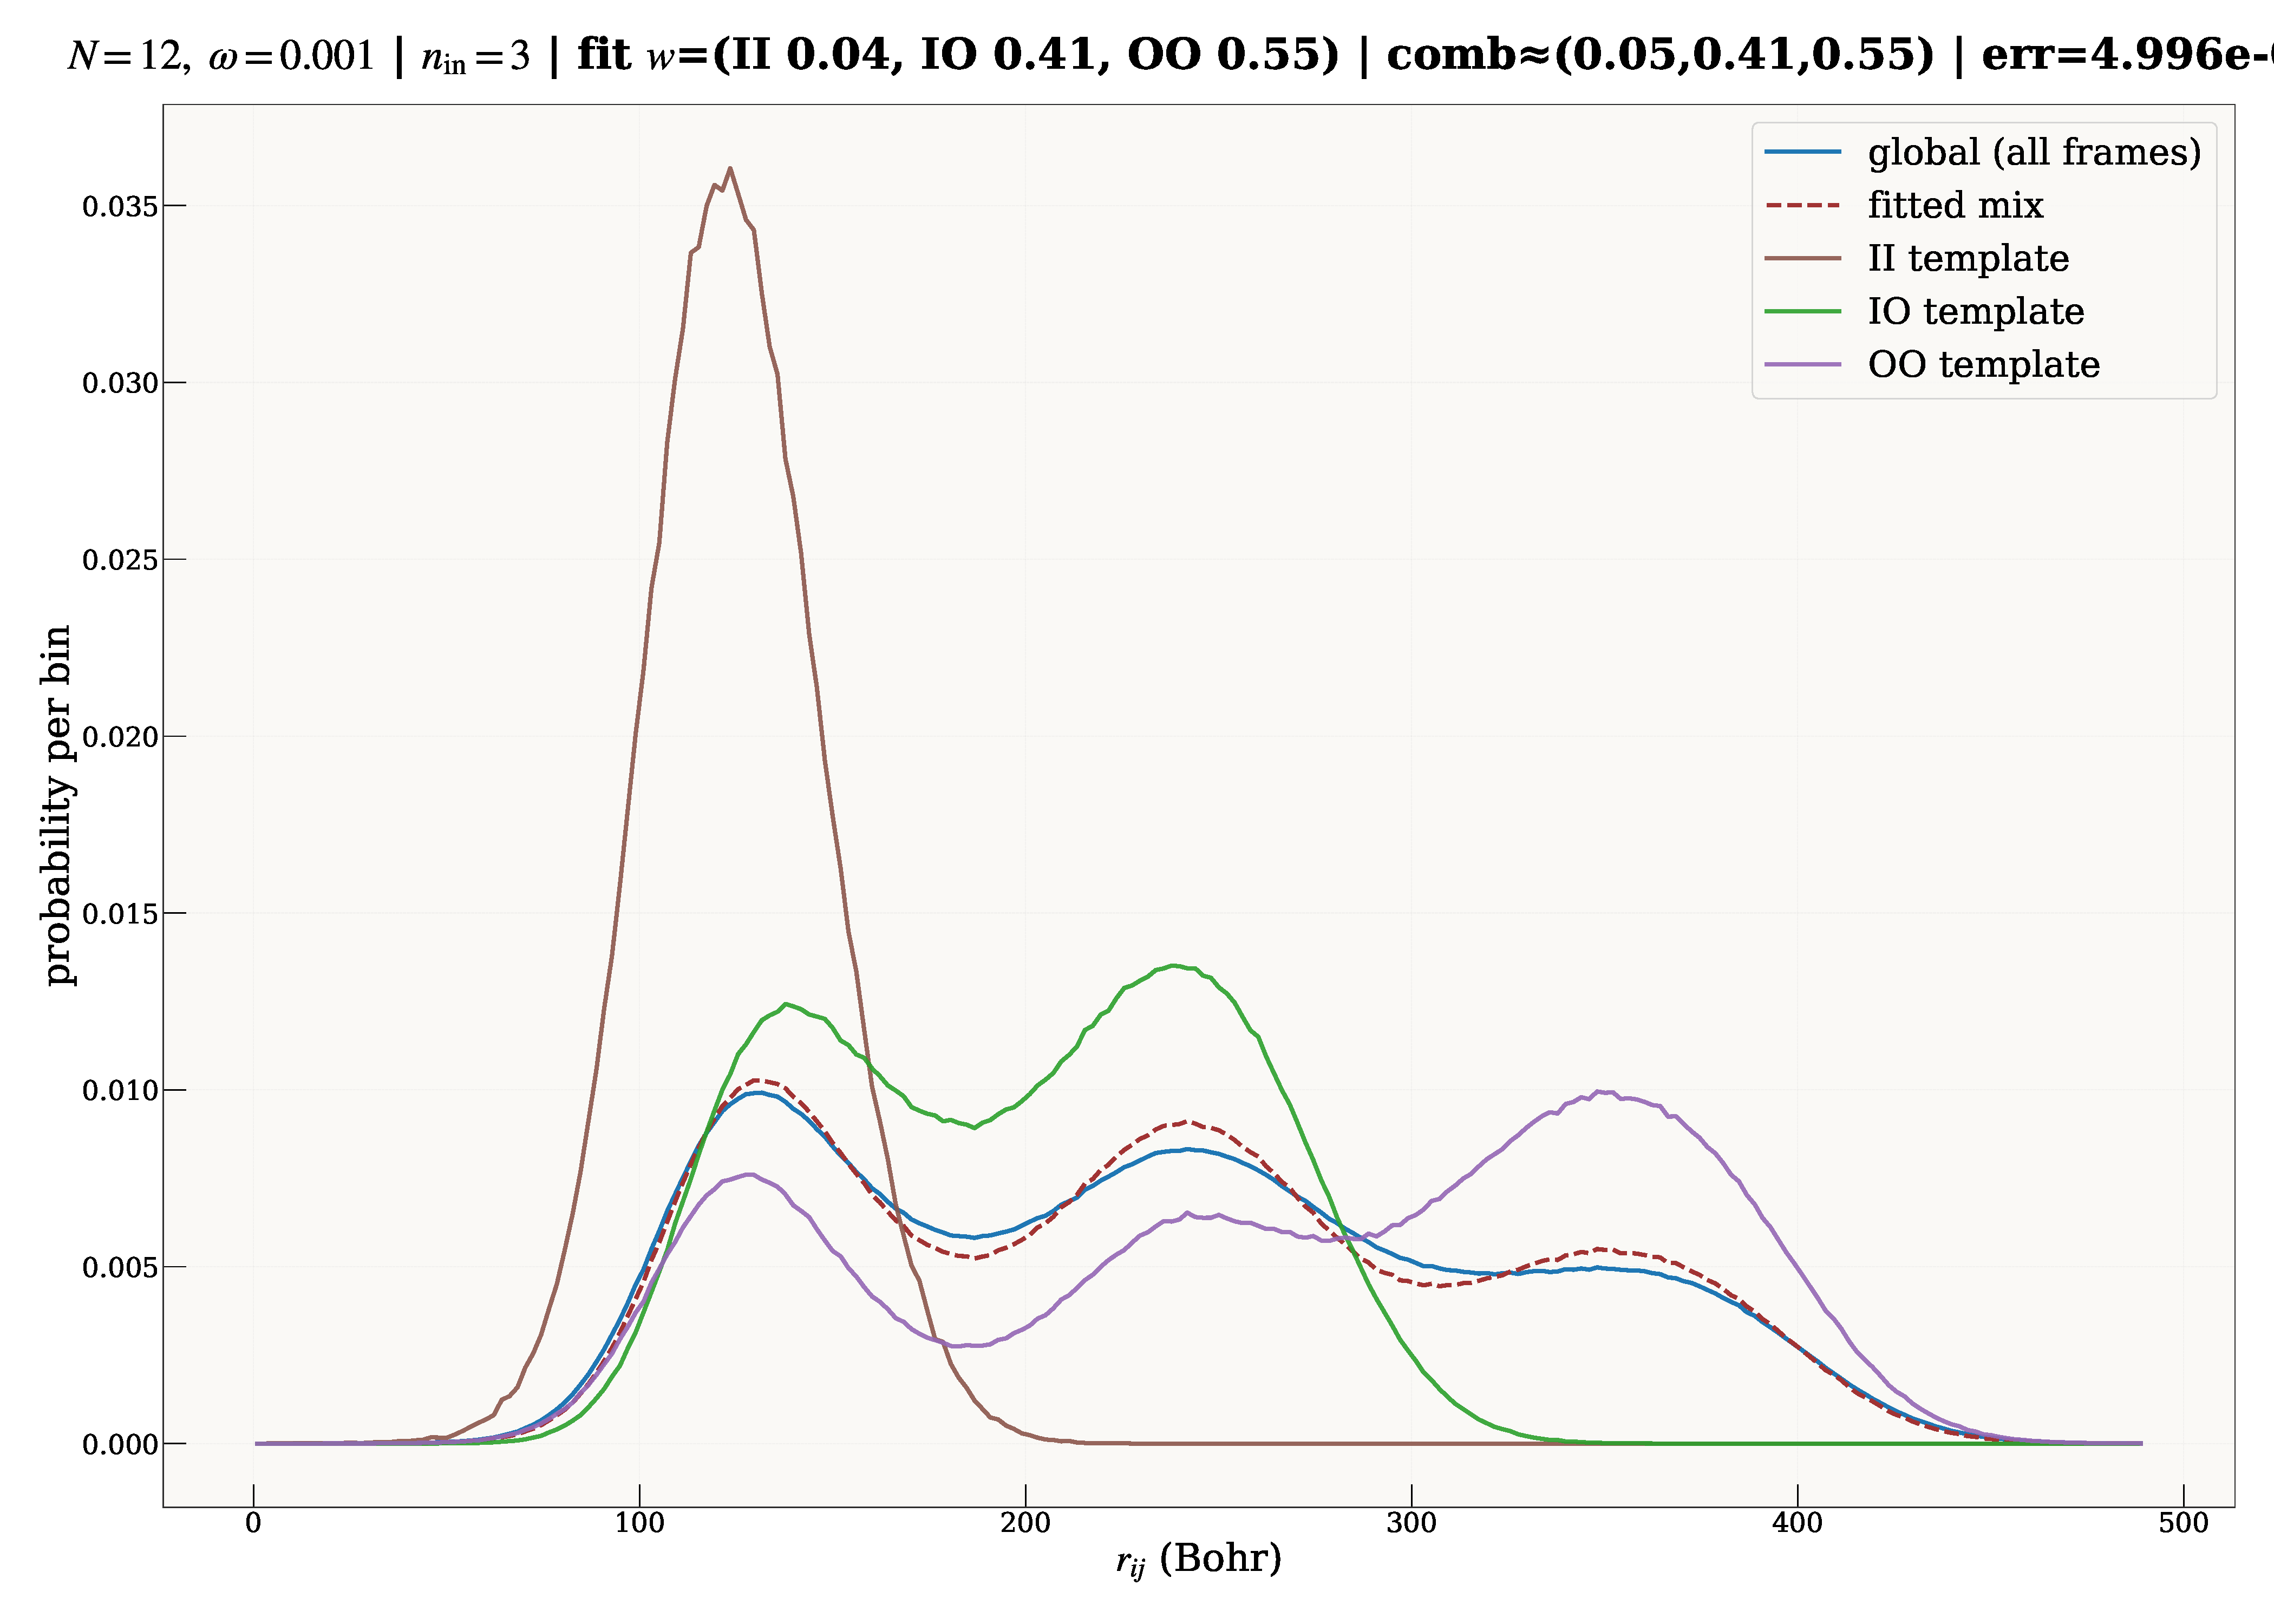
\includegraphics[width=0.8\textwidth]{mixfit_N12_w0.001_nin3.pdf}
  \caption[Shell-resolved reconstruction of $g(r)$, $N{=}12$]{Shell-resolved reconstruction of $g(r)$ at $\omega=10^{-3}$ for
  $N{=}12$.  The global pair distribution is reproduced by a convex mixture
  of inner--inner (II), inner--outer (IO) and outer--outer (OO) histograms
  with weights set by the observed $(n_{\rm in},n_{\rm out})$ statistics.}
  \label{fig:N12_w0001_decomposition}
\end{figure}

The polygon model reproduces the held-out pair distribution to cosine similarity
$0.987$--$0.999$ across the whole grid. The null reaches $0.936$--$0.996$, and the gap
between them, $\Delta\cos$, grows monotonically as the trap weakens at every particle
number---from $0.012$ to $0.058$ at $N{=}6$, from $0.006$ to $0.026$ at $N{=}12$, and from
$0.003$ to $0.010$ at $N{=}20$. Shell radii alone account for most of the pair structure at
strong confinement; angular order accounts for a growing remainder as the Wigner molecule
forms. This is the same transition the bond-order ratios of
Table~\ref{tab:shell-summary} record, measured on a different quantity and on held-out data.

\begin{table}[H]
\centering
\caption[Shell-model fit to the pair-distance distribution]{Shell-model fit to the pair-distance distribution. The empirical
$p_{\rm test}(r_{ij})$ on held-out frames is compared with (i) a \emph{polygon} model, in
which each detected shell is a regular $n_s$-gon with a per-frame global rotation and fitted
angular jitter, and (ii) a \emph{uniform-angle} null with the same fitted radial
distributions and no polygonal order. $\Delta\cos=\cos_{\rm poly}-\cos_{\rm uni}$ is what
angular order buys; $L^2_{\rm poly}$ is the polygon model's residual.}
\label{tab:shell-model-fit}
\small
\setlength{\tabcolsep}{6pt}
\begin{tabular}{ccl cccc}
\toprule
$N$ & $\omega$ & occ. & $\cos_{\rm poly}$ & $\cos_{\rm uni}$ & $\Delta\cos$ & $L^2_{\rm poly}$ \\
\midrule
 6 & $1.0$   & $(1,5)$    & $0.9988$ & $0.9866$ & $0.0122$ & $4.69\times10^{-3}$ \\
 6 & $0.5$   & $(1,5)$    & $0.9986$ & $0.9836$ & $0.0150$ & $5.09\times10^{-3}$ \\
 6 & $0.1$   & $(1,5)$    & $0.9974$ & $0.9741$ & $0.0234$ & $6.83\times10^{-3}$ \\
 6 & $0.01$  & $(1,5)$    & $0.9922$ & $0.9536$ & $0.0386$ & $1.14\times10^{-2}$ \\
 6 & $0.001$ & $(1,5)$    & $0.9942$ & $0.9358$ & $\mathbf{0.0585}$ & $1.04\times10^{-2}$ \\
\midrule
12 & $1.0$   & $(1,11)$   & $0.9993$ & $0.9937$ & $0.0056$ & $3.36\times10^{-3}$ \\
12 & $0.5$   & $(1,11)$   & $0.9990$ & $0.9927$ & $0.0063$ & $4.01\times10^{-3}$ \\
12 & $0.1$   & $(1,11)$   & $0.9980$ & $0.9896$ & $0.0085$ & $5.43\times10^{-3}$ \\
12 & $0.01$  & $(1,11)$   & $0.9929$ & $0.9805$ & $0.0124$ & $9.92\times10^{-3}$ \\
12 & $0.001$ & $(3,9)$    & $0.9868$ & $0.9604$ & $\mathbf{0.0264}$ & $1.34\times10^{-2}$ \\
\midrule
20 & $1.0$   & $(1,19)$   & $0.9992$ & $0.9964$ & $0.0028$ & $3.43\times10^{-3}$ \\
20 & $0.5$   & $(1,19)$   & $0.9990$ & $0.9958$ & $0.0032$ & $3.78\times10^{-3}$ \\
20 & $0.1$   & $(1,19)$   & $0.9982$ & $0.9942$ & $0.0040$ & $4.95\times10^{-3}$ \\
20 & $0.01$  & $(1,19)$   & $0.9947$ & $0.9900$ & $0.0047$ & $8.21\times10^{-3}$ \\
20 & $0.001$ & $(1,7,12)$ & $0.9915$ & $0.9820$ & $\mathbf{0.0095}$ & $1.02\times10^{-2}$ \\
\bottomrule
\end{tabular}
\end{table}

\section{The measured shell radius against the classical prediction}
\label{app:structural-tables:radius}

The classical minimum-energy configuration of six charges in a parabolic trap places five
of them on a ring of radius $1.334\,\omega^{-2/3}$
\cite{schweigert1994spectralpropertieschargedparticles,Kong_2002}. Nothing in the ansatz,
the training objective or the sampler knows that number, so the fitted outer-shell radius of
Table~\ref{tab:shell-summary} is an external check on the whole structural picture---and a
sharper one than the exponent fits of \S\ref{sec:wigner-radial}, because it tests a
prefactor as well as a power.

\begin{table}[H]
\centering
\caption[Measured shell radius against the classical prediction]{Fitted outer-shell radius of the $N{=}6$ $(1,5)$ molecule against the classical
Wigner ring $r_{\rm cl}=1.334\,\omega^{-2/3}$. Radii in Bohr.}
\label{tab:classical-radius}
\begin{tabular}{ccccc}
\toprule
$\omega$ & $r_{\rm shell}$ & $r_{\rm cl}$ & ratio \\
\midrule
$1.0$   & $1.66$   & $1.33$   & $1.247$ \\
$0.5$   & $2.52$   & $2.12$   & $1.188$ \\
$0.1$   & $6.80$   & $6.19$   & $1.098$ \\
$0.01$  & $29.65$  & $28.74$  & $1.032$ \\
$0.001$ & $135.67$ & $133.40$ & $1.017$ \\
\bottomrule
\end{tabular}
\end{table}

The ratio falls monotonically toward unity, reaching $1.017$ at $\omega=10^{-3}$: the
quantum ring sits $1.7\%$ outside the classical one at the weakest trap, and the excess
grows smoothly with confinement as zero-point motion pushes the shell outward. Fitting
$r_{\rm shell}\propto\omega^{\alpha}$ gives $\alpha=-0.637$ over the full grid and $-0.650$
over the weakest three confinements, against the classical $-2/3$.

Two remarks on why this quantity, rather than the $r_{\rm mode}$ of
Table~\ref{tab:radial-compact}, is the right one to compare. First, $r_{\rm mode}$ is the
mode of the \emph{single-particle} radial density, which for a $(1,5)$ topology mixes the
central electron with the ring and is therefore not the ring radius; fitting it gives
$\alpha\approx-0.58$ at $N{=}6$ and $-0.54$ at $N{=}2$ over the full grid, and approaches
$-2/3$ only on the weak-trap half. Second, the shell-resolved radius is the quantity the
physics-informed proposal of \S\ref{sec:kernel-q3-frontier} actually needs, so the agreement
recorded here is what licenses building a sampler out of it.

\chapter{Declaration on the Use of Artificial Intelligence}
\label{app:ai-declaration}

I used generative AI tools (ChatGPT, Claude and OpenAI Codex) during this thesis, from
March to September 2026, in three ways:
\begin{itemize}
  \item to revise and edit the text, including drafting revised passages, which I then
        reviewed, rewrote where needed and approved;
  \item to debate results, possible explanations and next steps;
  \item to patch and debug code. Commits made through these tools are marked as
        co-authored in the repository history.
\end{itemize}

The research questions, the scientific decisions and the conclusions are my own. No
numerical result was taken from generated text: reported values come from the cited
literature or from my saved calculations. I checked suggestions against derivations,
sources, code or saved results before using them, and rejected those I could not support.
I take full responsibility for the content, claims and references of this thesis.

\clearpage


%\bibliographystyle{johd}
\bibliographystyle{unsrtnat} 
\bibliography{references}

\end{document}
